\documentclass[twoside]{book}

% Packages required by doxygen
\usepackage{fixltx2e}
\usepackage{calc}
\usepackage{doxygen}
\usepackage[export]{adjustbox} % also loads graphicx
\usepackage{graphicx}
\usepackage[utf8]{inputenc}
\usepackage{makeidx}
\usepackage{multicol}
\usepackage{multirow}
\PassOptionsToPackage{warn}{textcomp}
\usepackage{textcomp}
\usepackage[nointegrals]{wasysym}
\usepackage[table]{xcolor}

% Font selection
\usepackage[T1]{fontenc}
\usepackage[scaled=.90]{helvet}
\usepackage{courier}
\usepackage{amssymb}
\usepackage{sectsty}
\renewcommand{\familydefault}{\sfdefault}
\allsectionsfont{%
  \fontseries{bc}\selectfont%
  \color{darkgray}%
}
\renewcommand{\DoxyLabelFont}{%
  \fontseries{bc}\selectfont%
  \color{darkgray}%
}
\newcommand{\+}{\discretionary{\mbox{\scriptsize$\hookleftarrow$}}{}{}}

% Page & text layout
\usepackage{geometry}
\geometry{%
  a4paper,%
  top=2.5cm,%
  bottom=2.5cm,%
  left=2.5cm,%
  right=2.5cm%
}
\tolerance=750
\hfuzz=15pt
\hbadness=750
\setlength{\emergencystretch}{15pt}
\setlength{\parindent}{0cm}
\setlength{\parskip}{3ex plus 2ex minus 2ex}
\makeatletter
\renewcommand{\paragraph}{%
  \@startsection{paragraph}{4}{0ex}{-1.0ex}{1.0ex}{%
    \normalfont\normalsize\bfseries\SS@parafont%
  }%
}
\renewcommand{\subparagraph}{%
  \@startsection{subparagraph}{5}{0ex}{-1.0ex}{1.0ex}{%
    \normalfont\normalsize\bfseries\SS@subparafont%
  }%
}
\makeatother

% Headers & footers
\usepackage{fancyhdr}
\pagestyle{fancyplain}
\fancyhead[LE]{\fancyplain{}{\bfseries\thepage}}
\fancyhead[CE]{\fancyplain{}{}}
\fancyhead[RE]{\fancyplain{}{\bfseries\leftmark}}
\fancyhead[LO]{\fancyplain{}{\bfseries\rightmark}}
\fancyhead[CO]{\fancyplain{}{}}
\fancyhead[RO]{\fancyplain{}{\bfseries\thepage}}
\fancyfoot[LE]{\fancyplain{}{}}
\fancyfoot[CE]{\fancyplain{}{}}
\fancyfoot[RE]{\fancyplain{}{\bfseries\scriptsize Generated by Doxygen }}
\fancyfoot[LO]{\fancyplain{}{\bfseries\scriptsize Generated by Doxygen }}
\fancyfoot[CO]{\fancyplain{}{}}
\fancyfoot[RO]{\fancyplain{}{}}
\renewcommand{\footrulewidth}{0.4pt}
\renewcommand{\chaptermark}[1]{%
  \markboth{#1}{}%
}
\renewcommand{\sectionmark}[1]{%
  \markright{\thesection\ #1}%
}

% Indices & bibliography
\usepackage{natbib}
\usepackage[titles]{tocloft}
\setcounter{tocdepth}{3}
\setcounter{secnumdepth}{5}
\makeindex

% Hyperlinks (required, but should be loaded last)
\usepackage{ifpdf}
\ifpdf
  \usepackage[pdftex,pagebackref=true]{hyperref}
\else
  \usepackage[ps2pdf,pagebackref=true]{hyperref}
\fi
\hypersetup{%
  colorlinks=true,%
  linkcolor=blue,%
  citecolor=blue,%
  unicode%
}

% Custom commands
\newcommand{\clearemptydoublepage}{%
  \newpage{\pagestyle{empty}\cleardoublepage}%
}

\usepackage{caption}
\captionsetup{labelsep=space,justification=centering,font={bf},singlelinecheck=off,skip=4pt,position=top}

%===== C O N T E N T S =====

\begin{document}

% Titlepage & ToC
\hypersetup{pageanchor=false,
             bookmarksnumbered=true,
             pdfencoding=unicode
            }
\pagenumbering{roman}
\begin{titlepage}
\vspace*{7cm}
\begin{center}%
{\Large My Project }\\
\vspace*{1cm}
{\large Generated by Doxygen 1.8.11}\\
\end{center}
\end{titlepage}
\clearemptydoublepage
\tableofcontents
\clearemptydoublepage
\pagenumbering{arabic}
\hypersetup{pageanchor=true}

%--- Begin generated contents ---
\chapter{My Personal Index Page}
\label{index}\hypertarget{index}{}\hypertarget{index_intro_sec}{}\section{Introduction}\label{index_intro_sec}
Braitenberg Vehicles Simulator\+: Iteration 2 
\chapter{Hierarchical Index}
\section{Class Hierarchy}
This inheritance list is sorted roughly, but not completely, alphabetically\+:\begin{DoxyCompactList}
\item \contentsline{section}{Arena}{\pageref{classArena}}{}
\item \contentsline{section}{arena\+\_\+params}{\pageref{structarena__params}}{}
\item \contentsline{section}{Arena\+Entity}{\pageref{classArenaEntity}}{}
\begin{DoxyCompactList}
\item \contentsline{section}{Arena\+Immobile\+Entity}{\pageref{classArenaImmobileEntity}}{}
\begin{DoxyCompactList}
\item \contentsline{section}{Food}{\pageref{classFood}}{}
\end{DoxyCompactList}
\item \contentsline{section}{Arena\+Mobile\+Entity}{\pageref{classArenaMobileEntity}}{}
\begin{DoxyCompactList}
\item \contentsline{section}{Light}{\pageref{classLight}}{}
\item \contentsline{section}{Robot}{\pageref{classRobot}}{}
\end{DoxyCompactList}
\end{DoxyCompactList}
\item \contentsline{section}{Controller}{\pageref{classController}}{}
\item \contentsline{section}{Entity\+Factory}{\pageref{classEntityFactory}}{}
\item Graphics\+App\begin{DoxyCompactList}
\item \contentsline{section}{Graphics\+Arena\+Viewer}{\pageref{classGraphicsArenaViewer}}{}
\end{DoxyCompactList}
\item \contentsline{section}{Motion\+Behavior}{\pageref{classMotionBehavior}}{}
\begin{DoxyCompactList}
\item \contentsline{section}{Motion\+Behavior\+Differential}{\pageref{classMotionBehaviorDifferential}}{}
\end{DoxyCompactList}
\item \contentsline{section}{Motion\+Handler}{\pageref{classMotionHandler}}{}
\begin{DoxyCompactList}
\item \contentsline{section}{Motion\+Handler\+Robot}{\pageref{classMotionHandlerRobot}}{}
\item \contentsline{section}{Motion\+Handler\+Robot\+Aggressive}{\pageref{classMotionHandlerRobotAggressive}}{}
\item \contentsline{section}{Motion\+Handler\+Robot\+Coward}{\pageref{classMotionHandlerRobotCoward}}{}
\item \contentsline{section}{Motion\+Handler\+Robot\+Explore}{\pageref{classMotionHandlerRobotExplore}}{}
\item \contentsline{section}{Motion\+Handler\+Robot\+Love}{\pageref{classMotionHandlerRobotLove}}{}
\end{DoxyCompactList}
\item \contentsline{section}{Pose}{\pageref{structPose}}{}
\item \contentsline{section}{Rgb\+Color}{\pageref{structRgbColor}}{}
\item \contentsline{section}{Sensor}{\pageref{classSensor}}{}
\begin{DoxyCompactList}
\item \contentsline{section}{Food\+Sensor}{\pageref{classFoodSensor}}{}
\item \contentsline{section}{Light\+Sensor}{\pageref{classLightSensor}}{}
\end{DoxyCompactList}
\item \contentsline{section}{Sensor\+Touch}{\pageref{classSensorTouch}}{}
\item \contentsline{section}{Wheel\+Velocity}{\pageref{structWheelVelocity}}{}
\end{DoxyCompactList}

\chapter{Class Index}
\section{Class List}
Here are the classes, structs, unions and interfaces with brief descriptions\+:\begin{DoxyCompactList}
\item\contentsline{section}{\hyperlink{classArena}{Arena} \\*The main class for the simulation of a 2D world with many entities running around }{\pageref{classArena}}{}
\item\contentsline{section}{\hyperlink{structarena__params}{arena\+\_\+params} \\*Struct holding parameters for initializing the \hyperlink{classArena}{Arena} }{\pageref{structarena__params}}{}
\item\contentsline{section}{\hyperlink{classArenaEntity}{Arena\+Entity} \\*A base class from which all \hyperlink{classArena}{Arena} entities inherit }{\pageref{classArenaEntity}}{}
\item\contentsline{section}{\hyperlink{classArenaImmobileEntity}{Arena\+Immobile\+Entity} \\*An immobile entity in the \hyperlink{classArena}{Arena} }{\pageref{classArenaImmobileEntity}}{}
\item\contentsline{section}{\hyperlink{classArenaMobileEntity}{Arena\+Mobile\+Entity} \\*A mobile entity in the \hyperlink{classArena}{Arena}, capable of updating its own position and/or velocity when asked by the simulation }{\pageref{classArenaMobileEntity}}{}
\item\contentsline{section}{\hyperlink{classBase}{Base} \\*Class representing a immobile base within the \hyperlink{classArena}{Arena} }{\pageref{classBase}}{}
\item\contentsline{section}{\hyperlink{classController}{Controller} \\*\hyperlink{classController}{Controller} that mediates \hyperlink{classArena}{Arena} and \hyperlink{classGraphicsArenaViewer}{Graphics\+Arena\+Viewer} communication }{\pageref{classController}}{}
\item\contentsline{section}{\hyperlink{classEntityFactory}{Entity\+Factory} \\*A factory for the instantiation of all types of arena entities }{\pageref{classEntityFactory}}{}
\item\contentsline{section}{\hyperlink{classGraphicsArenaViewer}{Graphics\+Arena\+Viewer} \\*An application that uses the Min\+Gfx library to open up a window that includes a few buttons for controlling the simulation and can be used to draw circles and other computer graphics }{\pageref{classGraphicsArenaViewer}}{}
\item\contentsline{section}{\hyperlink{classMotionBehavior}{Motion\+Behavior} \\*Class managing an \hyperlink{classArenaMobileEntity}{Arena\+Mobile\+Entity}\textquotesingle{}s position }{\pageref{classMotionBehavior}}{}
\item\contentsline{section}{\hyperlink{classMotionBehaviorDifferential}{Motion\+Behavior\+Differential} \\*A simple model of differential drive kinematics based on the notes here\+: $\sim$https\+://chess.eecs.\+berkeley.\+edu/eecs149/documentation/differential\+Drive.pdf$\sim$ }{\pageref{classMotionBehaviorDifferential}}{}
\item\contentsline{section}{\hyperlink{classMotionHandler}{Motion\+Handler} \\*\hyperlink{classBase}{Base} class for managing the pose and wheel velocity of the entity }{\pageref{classMotionHandler}}{}
\item\contentsline{section}{\hyperlink{classMotionHandlerRobot}{Motion\+Handler\+Robot} \\*Class managing a \hyperlink{classRobot}{Robot}\textquotesingle{}s and obstacle\textquotesingle{}s speed and heading angle based on collisions and user inputs }{\pageref{classMotionHandlerRobot}}{}
\item\contentsline{section}{\hyperlink{classObstacle}{Obstacle} \\*Class representing an mobile obstacle within the \hyperlink{classArena}{Arena} }{\pageref{classObstacle}}{}
\item\contentsline{section}{\hyperlink{structPose}{Pose} \\*A simple representation of the position/orientation of an entity within the \hyperlink{classArena}{Arena} }{\pageref{structPose}}{}
\item\contentsline{section}{\hyperlink{structRgbColor}{Rgb\+Color} \\*Struct representing a rgb\+\_\+color }{\pageref{structRgbColor}}{}
\item\contentsline{section}{\hyperlink{classRobot}{Robot} \\*Class representing a robot within the arena }{\pageref{classRobot}}{}
\item\contentsline{section}{\hyperlink{classSensorTouch}{Sensor\+Touch} \\*Class representing a touch sensor }{\pageref{classSensorTouch}}{}
\item\contentsline{section}{\hyperlink{structWheelVelocity}{Wheel\+Velocity} \\*A simple representation of the position/orientation of an entity within the \hyperlink{classArena}{Arena} }{\pageref{structWheelVelocity}}{}
\end{DoxyCompactList}

\chapter{File Index}
\section{File List}
Here is a list of all documented files with brief descriptions\+:\begin{DoxyCompactList}
\item\contentsline{section}{src/\hyperlink{arena_8cc}{arena.\+cc} }{\pageref{arena_8cc}}{}
\item\contentsline{section}{src/\hyperlink{arena_8h}{arena.\+h} }{\pageref{arena_8h}}{}
\item\contentsline{section}{src/\hyperlink{arena__entity_8h}{arena\+\_\+entity.\+h} }{\pageref{arena__entity_8h}}{}
\item\contentsline{section}{src/\hyperlink{arena__immobile__entity_8h}{arena\+\_\+immobile\+\_\+entity.\+h} }{\pageref{arena__immobile__entity_8h}}{}
\item\contentsline{section}{src/\hyperlink{arena__mobile__entity_8h}{arena\+\_\+mobile\+\_\+entity.\+h} }{\pageref{arena__mobile__entity_8h}}{}
\item\contentsline{section}{src/\hyperlink{arena__params_8h}{arena\+\_\+params.\+h} }{\pageref{arena__params_8h}}{}
\item\contentsline{section}{src/\hyperlink{common_8h}{common.\+h} }{\pageref{common_8h}}{}
\item\contentsline{section}{src/\hyperlink{communication_8h}{communication.\+h} }{\pageref{communication_8h}}{}
\item\contentsline{section}{src/\hyperlink{controller_8cc}{controller.\+cc} }{\pageref{controller_8cc}}{}
\item\contentsline{section}{src/\hyperlink{controller_8h}{controller.\+h} }{\pageref{controller_8h}}{}
\item\contentsline{section}{src/\hyperlink{entity__factory_8cc}{entity\+\_\+factory.\+cc} }{\pageref{entity__factory_8cc}}{}
\item\contentsline{section}{src/\hyperlink{entity__factory_8h}{entity\+\_\+factory.\+h} }{\pageref{entity__factory_8h}}{}
\item\contentsline{section}{src/\hyperlink{entity__type_8h}{entity\+\_\+type.\+h} }{\pageref{entity__type_8h}}{}
\item\contentsline{section}{src/\hyperlink{food_8cc}{food.\+cc} }{\pageref{food_8cc}}{}
\item\contentsline{section}{src/\hyperlink{food_8h}{food.\+h} }{\pageref{food_8h}}{}
\item\contentsline{section}{src/\hyperlink{food__sensor_8cc}{food\+\_\+sensor.\+cc} }{\pageref{food__sensor_8cc}}{}
\item\contentsline{section}{src/\hyperlink{food__sensor_8h}{food\+\_\+sensor.\+h} }{\pageref{food__sensor_8h}}{}
\item\contentsline{section}{src/\hyperlink{graphics__arena__viewer_8cc}{graphics\+\_\+arena\+\_\+viewer.\+cc} }{\pageref{graphics__arena__viewer_8cc}}{}
\item\contentsline{section}{src/\hyperlink{graphics__arena__viewer_8h}{graphics\+\_\+arena\+\_\+viewer.\+h} }{\pageref{graphics__arena__viewer_8h}}{}
\item\contentsline{section}{src/\hyperlink{light_8cc}{light.\+cc} }{\pageref{light_8cc}}{}
\item\contentsline{section}{src/\hyperlink{light_8h}{light.\+h} }{\pageref{light_8h}}{}
\item\contentsline{section}{src/\hyperlink{light__sensor_8cc}{light\+\_\+sensor.\+cc} }{\pageref{light__sensor_8cc}}{}
\item\contentsline{section}{src/\hyperlink{light__sensor_8h}{light\+\_\+sensor.\+h} }{\pageref{light__sensor_8h}}{}
\item\contentsline{section}{src/\hyperlink{main_8cc}{main.\+cc} }{\pageref{main_8cc}}{}
\item\contentsline{section}{src/\hyperlink{mainpage_8h}{mainpage.\+h} }{\pageref{mainpage_8h}}{}
\item\contentsline{section}{src/\hyperlink{motion__behavior_8cc}{motion\+\_\+behavior.\+cc} }{\pageref{motion__behavior_8cc}}{}
\item\contentsline{section}{src/\hyperlink{motion__behavior_8h}{motion\+\_\+behavior.\+h} }{\pageref{motion__behavior_8h}}{}
\item\contentsline{section}{src/\hyperlink{motion__behavior__differential_8h}{motion\+\_\+behavior\+\_\+differential.\+h} }{\pageref{motion__behavior__differential_8h}}{}
\item\contentsline{section}{src/\hyperlink{motion__handler_8cc}{motion\+\_\+handler.\+cc} }{\pageref{motion__handler_8cc}}{}
\item\contentsline{section}{src/\hyperlink{motion__handler_8h}{motion\+\_\+handler.\+h} }{\pageref{motion__handler_8h}}{}
\item\contentsline{section}{src/\hyperlink{motion__handler__robot_8cc}{motion\+\_\+handler\+\_\+robot.\+cc} }{\pageref{motion__handler__robot_8cc}}{}
\item\contentsline{section}{src/\hyperlink{motion__handler__robot_8h}{motion\+\_\+handler\+\_\+robot.\+h} }{\pageref{motion__handler__robot_8h}}{}
\item\contentsline{section}{src/\hyperlink{motion__handler__robot__aggressive_8cc}{motion\+\_\+handler\+\_\+robot\+\_\+aggressive.\+cc} }{\pageref{motion__handler__robot__aggressive_8cc}}{}
\item\contentsline{section}{src/\hyperlink{motion__handler__robot__aggressive_8h}{motion\+\_\+handler\+\_\+robot\+\_\+aggressive.\+h} }{\pageref{motion__handler__robot__aggressive_8h}}{}
\item\contentsline{section}{src/\hyperlink{motion__handler__robot__coward_8cc}{motion\+\_\+handler\+\_\+robot\+\_\+coward.\+cc} }{\pageref{motion__handler__robot__coward_8cc}}{}
\item\contentsline{section}{src/\hyperlink{motion__handler__robot__coward_8h}{motion\+\_\+handler\+\_\+robot\+\_\+coward.\+h} }{\pageref{motion__handler__robot__coward_8h}}{}
\item\contentsline{section}{src/\hyperlink{motion__handler__robot__explore_8cc}{motion\+\_\+handler\+\_\+robot\+\_\+explore.\+cc} }{\pageref{motion__handler__robot__explore_8cc}}{}
\item\contentsline{section}{src/\hyperlink{motion__handler__robot__explore_8h}{motion\+\_\+handler\+\_\+robot\+\_\+explore.\+h} }{\pageref{motion__handler__robot__explore_8h}}{}
\item\contentsline{section}{src/\hyperlink{motion__handler__robot__love_8cc}{motion\+\_\+handler\+\_\+robot\+\_\+love.\+cc} }{\pageref{motion__handler__robot__love_8cc}}{}
\item\contentsline{section}{src/\hyperlink{motion__handler__robot__love_8h}{motion\+\_\+handler\+\_\+robot\+\_\+love.\+h} }{\pageref{motion__handler__robot__love_8h}}{}
\item\contentsline{section}{src/\hyperlink{params_8h}{params.\+h} }{\pageref{params_8h}}{}
\item\contentsline{section}{src/\hyperlink{pose_8h}{pose.\+h} }{\pageref{pose_8h}}{}
\item\contentsline{section}{src/\hyperlink{rgb__color_8cc}{rgb\+\_\+color.\+cc} }{\pageref{rgb__color_8cc}}{}
\item\contentsline{section}{src/\hyperlink{rgb__color_8h}{rgb\+\_\+color.\+h} }{\pageref{rgb__color_8h}}{}
\item\contentsline{section}{src/\hyperlink{robot_8cc}{robot.\+cc} }{\pageref{robot_8cc}}{}
\item\contentsline{section}{src/\hyperlink{robot_8h}{robot.\+h} }{\pageref{robot_8h}}{}
\item\contentsline{section}{src/\hyperlink{robot__type_8h}{robot\+\_\+type.\+h} }{\pageref{robot__type_8h}}{}
\item\contentsline{section}{src/\hyperlink{sensor_8cc}{sensor.\+cc} }{\pageref{sensor_8cc}}{}
\item\contentsline{section}{src/\hyperlink{sensor_8h}{sensor.\+h} }{\pageref{sensor_8h}}{}
\item\contentsline{section}{src/\hyperlink{sensor__touch_8cc}{sensor\+\_\+touch.\+cc} }{\pageref{sensor__touch_8cc}}{}
\item\contentsline{section}{src/\hyperlink{sensor__touch_8h}{sensor\+\_\+touch.\+h} }{\pageref{sensor__touch_8h}}{}
\item\contentsline{section}{src/\hyperlink{sensor__type_8h}{sensor\+\_\+type.\+h} }{\pageref{sensor__type_8h}}{}
\item\contentsline{section}{src/\hyperlink{wheel__velocity_8h}{wheel\+\_\+velocity.\+h} }{\pageref{wheel__velocity_8h}}{}
\end{DoxyCompactList}

\chapter{Class Documentation}
\hypertarget{class_arena}{}\section{Arena Class Reference}
\label{class_arena}\index{Arena@{Arena}}


The main class for the simulation of a 2D world with many entities running around.  




{\ttfamily \#include $<$arena.\+h$>$}

\subsection*{Public Member Functions}
\begin{DoxyCompactItemize}
\item 
\hyperlink{class_arena_ac442d519facc5feebfd7612a53817e9a}{Arena} (const struct \hyperlink{structarena__params}{arena\+\_\+params} $\ast$const params)
\begin{DoxyCompactList}\small\item\em \hyperlink{class_arena}{Arena}\textquotesingle{}s constructor. \end{DoxyCompactList}\item 
\hyperlink{class_arena_ae21b399e9e3f6b8ac4ecc44d7d1667fc}{$\sim$\+Arena} ()\hypertarget{class_arena_ae21b399e9e3f6b8ac4ecc44d7d1667fc}{}\label{class_arena_ae21b399e9e3f6b8ac4ecc44d7d1667fc}

\begin{DoxyCompactList}\small\item\em \hyperlink{class_arena}{Arena}\textquotesingle{}s destructor. {\ttfamily delete} all entities created. \end{DoxyCompactList}\item 
void \hyperlink{class_arena_ad92d8b2e1593b652445e31d173977fc6}{Advance\+Time} (double dt)
\begin{DoxyCompactList}\small\item\em Advance the simulation by the specified \# of steps. \end{DoxyCompactList}\item 
void \hyperlink{class_arena_a0012b0774ae6642a1a559b97ca335c4b}{Add\+Robot} (Robot\+Type rt, int quantity)
\begin{DoxyCompactList}\small\item\em function to add a robot to the arena \end{DoxyCompactList}\item 
void \hyperlink{class_arena_a9e00ef1a079d49d648359952fcfaa9f3}{Add\+Entity} (Entity\+Type type, int quantity)
\begin{DoxyCompactList}\small\item\em function to add an entity to the arena \end{DoxyCompactList}\item 
void \hyperlink{class_arena_a3166b6d49cc1fa5a526317ee55eefa16}{Register\+Light\+Sensor\+Observer} (\hyperlink{class_light_sensor}{Light\+Sensor} $\ast$ob)
\begin{DoxyCompactList}\small\item\em registers the light sensors of the robot as observes of arena \end{DoxyCompactList}\item 
void \hyperlink{class_arena_acb467d8cd9635b2dd0a3a22f08f543c7}{Register\+Food\+Sensor\+Observer} (\hyperlink{class_food_sensor}{Food\+Sensor} $\ast$ob)
\begin{DoxyCompactList}\small\item\em registers the food sensors of the robot as observes of arena \end{DoxyCompactList}\item 
void \hyperlink{class_arena_a694758081979e9944031000a375a3a6a}{Notify} ()\hypertarget{class_arena_a694758081979e9944031000a375a3a6a}{}\label{class_arena_a694758081979e9944031000a375a3a6a}

\begin{DoxyCompactList}\small\item\em notify the observes of the new postions of the foods and lights \end{DoxyCompactList}\item 
void \hyperlink{class_arena_a16fac8e4b2399fcf0db01a9722069c33}{Accept\+Command} (Communication com)\hypertarget{class_arena_a16fac8e4b2399fcf0db01a9722069c33}{}\label{class_arena_a16fac8e4b2399fcf0db01a9722069c33}

\begin{DoxyCompactList}\small\item\em translates communication from the controller to action in the arena \end{DoxyCompactList}\item 
void \hyperlink{class_arena_a95e295d03a14385f4402a8e839fbae9b}{Reset} ()\hypertarget{class_arena_a95e295d03a14385f4402a8e839fbae9b}{}\label{class_arena_a95e295d03a14385f4402a8e839fbae9b}

\begin{DoxyCompactList}\small\item\em Reset all entities in \hyperlink{class_arena}{Arena}. \end{DoxyCompactList}\item 
class \hyperlink{class_robot}{Robot} $\ast$ \hyperlink{class_arena_af9b489317866a4541c6531acb63602c3}{robot} () const 
\begin{DoxyCompactList}\small\item\em Get the \hyperlink{class_robot}{Robot} in \hyperlink{class_arena}{Arena}. \end{DoxyCompactList}\item 
\hyperlink{class_arena}{Arena} \& \hyperlink{class_arena_aa977a50aa4a5570a2a553705f1909e9b}{operator=} (const \hyperlink{class_arena}{Arena} \&other)=delete\hypertarget{class_arena_aa977a50aa4a5570a2a553705f1909e9b}{}\label{class_arena_aa977a50aa4a5570a2a553705f1909e9b}

\begin{DoxyCompactList}\small\item\em Under certain circumstance, the compiler requires that the assignment operator is not defined. This {\ttfamily deletes} the default assignment operator. \end{DoxyCompactList}\item 
\hyperlink{class_arena_afce6e35e1470823539dc9194bef77499}{Arena} (const \hyperlink{class_arena}{Arena} \&other)=delete\hypertarget{class_arena_afce6e35e1470823539dc9194bef77499}{}\label{class_arena_afce6e35e1470823539dc9194bef77499}

\begin{DoxyCompactList}\small\item\em Under certain circumstance, the compiler requires that the copy constructor is not defined. This {\ttfamily deletes} the default copy constructor. \end{DoxyCompactList}\item 
bool \hyperlink{class_arena_ab4479b0268867602d0c4b510d5f99aff}{Is\+Colliding} (\hyperlink{class_arena_mobile_entity}{Arena\+Mobile\+Entity} $\ast$const mobile\+\_\+e, \hyperlink{class_arena_entity}{Arena\+Entity} $\ast$const other\+\_\+e)
\begin{DoxyCompactList}\small\item\em Determine if two entities have collided in the \hyperlink{class_arena}{Arena}. Collision is defined as the distance between two entities being less than the sum of their radii. \end{DoxyCompactList}\item 
void \hyperlink{class_arena_a2506fab770b6070d8f061bcab4c65138}{Adjust\+Entity\+Overlap} (\hyperlink{class_arena_mobile_entity}{Arena\+Mobile\+Entity} $\ast$const mobile\+\_\+e, \hyperlink{class_arena_entity}{Arena\+Entity} $\ast$const other\+\_\+e)\hypertarget{class_arena_a2506fab770b6070d8f061bcab4c65138}{}\label{class_arena_a2506fab770b6070d8f061bcab4c65138}

\begin{DoxyCompactList}\small\item\em Move the mobile entity to the edge of the other without overlap. Without this, entities tend to get stuck inside one another. \end{DoxyCompactList}\item 
Entity\+Type \hyperlink{class_arena_a7b72cf7688ee6ab1395bf438663bc1da}{Get\+Collision\+Wall} (\hyperlink{class_arena_mobile_entity}{Arena\+Mobile\+Entity} $\ast$const ent)
\begin{DoxyCompactList}\small\item\em Determine if a particular entity has gone out of the boundaries of the simulation (i.\+e. has collided with any one of the walls). \end{DoxyCompactList}\item 
void \hyperlink{class_arena_a51c1e99dfd9a618c6041fd22d0a11959}{Adjust\+Wall\+Overlap} (\hyperlink{class_arena_mobile_entity}{Arena\+Mobile\+Entity} $\ast$const ent, Entity\+Type wall)\hypertarget{class_arena_a51c1e99dfd9a618c6041fd22d0a11959}{}\label{class_arena_a51c1e99dfd9a618c6041fd22d0a11959}

\begin{DoxyCompactList}\small\item\em Move the entity to the edge of the wall without overlap. Without this, entities tend to get stuck in walls. \end{DoxyCompactList}\item 
void \hyperlink{class_arena_a682ec81cb30e36e5bb801b3388bcb494}{Update\+Entities\+Timestep} ()
\begin{DoxyCompactList}\small\item\em Update all entities for a single timestep. \end{DoxyCompactList}\item 
void \hyperlink{class_arena_a700c436c43cd6c692b0e357dac94c507}{Update\+Game\+Status} ()
\begin{DoxyCompactList}\small\item\em Update the game status to win or loss. \end{DoxyCompactList}\item 
void {\bfseries Config\+Arena} (int robotnum, double coward\+\_\+percent, int lightnum, int foodnum, double sensitivity, bool food\+\_\+on\+\_\+)\hypertarget{class_arena_ad65f82d31e5d0fc7a859a809222fe53f}{}\label{class_arena_ad65f82d31e5d0fc7a859a809222fe53f}

\item 
std\+::vector$<$ class \hyperlink{class_arena_entity}{Arena\+Entity} $\ast$ $>$ {\bfseries get\+\_\+entities} () const \hypertarget{class_arena_aabb4ffe05aefc71ee10d47b191963fe5}{}\label{class_arena_aabb4ffe05aefc71ee10d47b191963fe5}

\item 
double {\bfseries get\+\_\+x\+\_\+dim} ()\hypertarget{class_arena_a5e3be20f2c67338a5a684b85a66f6b96}{}\label{class_arena_a5e3be20f2c67338a5a684b85a66f6b96}

\item 
double {\bfseries get\+\_\+y\+\_\+dim} ()\hypertarget{class_arena_a35737d65ff32f2bd5871f0bdfbc10a85}{}\label{class_arena_a35737d65ff32f2bd5871f0bdfbc10a85}

\item 
int {\bfseries get\+\_\+game\+\_\+status} () const \hypertarget{class_arena_a6d196837daa08a2618c3ff6e0a741b25}{}\label{class_arena_a6d196837daa08a2618c3ff6e0a741b25}

\item 
void {\bfseries set\+\_\+game\+\_\+status} (int status)\hypertarget{class_arena_ac8e8b3438db02aa5395f7fcb537ed952}{}\label{class_arena_ac8e8b3438db02aa5395f7fcb537ed952}

\end{DoxyCompactItemize}


\subsection{Detailed Description}
The main class for the simulation of a 2D world with many entities running around. 

While \hyperlink{class_graphics_arena_viewer}{Graphics\+Arena\+Viewer} handles the graphics, \hyperlink{class_arena}{Arena} handles all the data and all the entities (it is the model of M\+VC). It manages the interaction among the entities in the \hyperlink{class_arena}{Arena}. 

\subsection{Constructor \& Destructor Documentation}
\index{Arena@{Arena}!Arena@{Arena}}
\index{Arena@{Arena}!Arena@{Arena}}
\subsubsection[{\texorpdfstring{Arena(const struct arena\+\_\+params $\ast$const params)}{Arena(const struct arena_params *const params)}}]{\setlength{\rightskip}{0pt plus 5cm}Arena\+::\+Arena (
\begin{DoxyParamCaption}
\item[{const struct {\bf arena\+\_\+params} $\ast$const}]{params}
\end{DoxyParamCaption}
)\hspace{0.3cm}{\ttfamily [explicit]}}\hypertarget{class_arena_ac442d519facc5feebfd7612a53817e9a}{}\label{class_arena_ac442d519facc5feebfd7612a53817e9a}


\hyperlink{class_arena}{Arena}\textquotesingle{}s constructor. 


\begin{DoxyParams}{Parameters}
{\em params} & A \hyperlink{structarena__params}{arena\+\_\+params} passed down from \hyperlink{main_8cc}{main.\+cc} for the initialization of \hyperlink{class_arena}{Arena} and the entities therein.\\
\hline
\end{DoxyParams}
Initialize all private variables and entities. 

\subsection{Member Function Documentation}
\index{Arena@{Arena}!Add\+Entity@{Add\+Entity}}
\index{Add\+Entity@{Add\+Entity}!Arena@{Arena}}
\subsubsection[{\texorpdfstring{Add\+Entity(\+Entity\+Type type, int quantity)}{AddEntity(EntityType type, int quantity)}}]{\setlength{\rightskip}{0pt plus 5cm}void Arena\+::\+Add\+Entity (
\begin{DoxyParamCaption}
\item[{Entity\+Type}]{type, }
\item[{int}]{quantity}
\end{DoxyParamCaption}
)}\hypertarget{class_arena_a9e00ef1a079d49d648359952fcfaa9f3}{}\label{class_arena_a9e00ef1a079d49d648359952fcfaa9f3}


function to add an entity to the arena 


\begin{DoxyParams}{Parameters}
{\em type} & of the entity (food or light) \\
\hline
\end{DoxyParams}
\index{Arena@{Arena}!Add\+Robot@{Add\+Robot}}
\index{Add\+Robot@{Add\+Robot}!Arena@{Arena}}
\subsubsection[{\texorpdfstring{Add\+Robot(\+Robot\+Type rt, int quantity)}{AddRobot(RobotType rt, int quantity)}}]{\setlength{\rightskip}{0pt plus 5cm}void Arena\+::\+Add\+Robot (
\begin{DoxyParamCaption}
\item[{Robot\+Type}]{rt, }
\item[{int}]{quantity}
\end{DoxyParamCaption}
)}\hypertarget{class_arena_a0012b0774ae6642a1a559b97ca335c4b}{}\label{class_arena_a0012b0774ae6642a1a559b97ca335c4b}


function to add a robot to the arena 


\begin{DoxyParams}{Parameters}
{\em rt} & the behavior of the robot\textquotesingle{}s motion toward sensors \\
\hline
\end{DoxyParams}
\index{Arena@{Arena}!Advance\+Time@{Advance\+Time}}
\index{Advance\+Time@{Advance\+Time}!Arena@{Arena}}
\subsubsection[{\texorpdfstring{Advance\+Time(double dt)}{AdvanceTime(double dt)}}]{\setlength{\rightskip}{0pt plus 5cm}void Arena\+::\+Advance\+Time (
\begin{DoxyParamCaption}
\item[{double}]{dt}
\end{DoxyParamCaption}
)}\hypertarget{class_arena_ad92d8b2e1593b652445e31d173977fc6}{}\label{class_arena_ad92d8b2e1593b652445e31d173977fc6}


Advance the simulation by the specified \# of steps. 


\begin{DoxyParams}[1]{Parameters}
\mbox{\tt in}  & {\em dt} & The \# of steps to increment by. This is practically unused because the arena state is advanced incrementally at a fixed rate.\\
\hline
\end{DoxyParams}
If {\ttfamily dt == 0}, {\ttfamily return} immediately. Otherwise calls \hyperlink{class_arena_a682ec81cb30e36e5bb801b3388bcb494}{Arena\+::\+Update\+Entities\+Timestep()} once. \index{Arena@{Arena}!Get\+Collision\+Wall@{Get\+Collision\+Wall}}
\index{Get\+Collision\+Wall@{Get\+Collision\+Wall}!Arena@{Arena}}
\subsubsection[{\texorpdfstring{Get\+Collision\+Wall(\+Arena\+Mobile\+Entity $\ast$const ent)}{GetCollisionWall(ArenaMobileEntity *const ent)}}]{\setlength{\rightskip}{0pt plus 5cm}Entity\+Type Arena\+::\+Get\+Collision\+Wall (
\begin{DoxyParamCaption}
\item[{{\bf Arena\+Mobile\+Entity} $\ast$const}]{ent}
\end{DoxyParamCaption}
)}\hypertarget{class_arena_a7b72cf7688ee6ab1395bf438663bc1da}{}\label{class_arena_a7b72cf7688ee6ab1395bf438663bc1da}


Determine if a particular entity has gone out of the boundaries of the simulation (i.\+e. has collided with any one of the walls). 


\begin{DoxyParams}[1]{Parameters}
 & {\em ent} & The entity to check. \\
\hline
\mbox{\tt out}  & {\em An} & entity type signifying wall (e.\+g. k\+Right\+Wall). k\+Undefined if no collision.\\
\hline
\end{DoxyParams}
The checked entity\textquotesingle{}s position will be updated to a \char`\"{}back-\/off position\char`\"{} so that it won\textquotesingle{}t get stuck into a wall. The calculation of the \char`\"{}back-\/off
position\char`\"{} is technically not accurate, but good enough for our purpose. \index{Arena@{Arena}!Is\+Colliding@{Is\+Colliding}}
\index{Is\+Colliding@{Is\+Colliding}!Arena@{Arena}}
\subsubsection[{\texorpdfstring{Is\+Colliding(\+Arena\+Mobile\+Entity $\ast$const mobile\+\_\+e, Arena\+Entity $\ast$const other\+\_\+e)}{IsColliding(ArenaMobileEntity *const mobile_e, ArenaEntity *const other_e)}}]{\setlength{\rightskip}{0pt plus 5cm}bool Arena\+::\+Is\+Colliding (
\begin{DoxyParamCaption}
\item[{{\bf Arena\+Mobile\+Entity} $\ast$const}]{mobile\+\_\+e, }
\item[{{\bf Arena\+Entity} $\ast$const}]{other\+\_\+e}
\end{DoxyParamCaption}
)}\hypertarget{class_arena_ab4479b0268867602d0c4b510d5f99aff}{}\label{class_arena_ab4479b0268867602d0c4b510d5f99aff}


Determine if two entities have collided in the \hyperlink{class_arena}{Arena}. Collision is defined as the distance between two entities being less than the sum of their radii. 


\begin{DoxyParams}[1]{Parameters}
 & {\em mobile\+\_\+e} & This entity is definitely moving. \\
\hline
 & {\em other\+\_\+e} & This entity might be mobile or immobile. \\
\hline
\mbox{\tt out}  & {\em True} & if entities overlapping. \\
\hline
\end{DoxyParams}
\index{Arena@{Arena}!Register\+Food\+Sensor\+Observer@{Register\+Food\+Sensor\+Observer}}
\index{Register\+Food\+Sensor\+Observer@{Register\+Food\+Sensor\+Observer}!Arena@{Arena}}
\subsubsection[{\texorpdfstring{Register\+Food\+Sensor\+Observer(\+Food\+Sensor $\ast$ob)}{RegisterFoodSensorObserver(FoodSensor *ob)}}]{\setlength{\rightskip}{0pt plus 5cm}void Arena\+::\+Register\+Food\+Sensor\+Observer (
\begin{DoxyParamCaption}
\item[{{\bf Food\+Sensor} $\ast$}]{ob}
\end{DoxyParamCaption}
)}\hypertarget{class_arena_acb467d8cd9635b2dd0a3a22f08f543c7}{}\label{class_arena_acb467d8cd9635b2dd0a3a22f08f543c7}


registers the food sensors of the robot as observes of arena 


\begin{DoxyParams}[1]{Parameters}
\mbox{\tt in}  & {\em ob} & The foodsensor of the robot \\
\hline
\end{DoxyParams}
\index{Arena@{Arena}!Register\+Light\+Sensor\+Observer@{Register\+Light\+Sensor\+Observer}}
\index{Register\+Light\+Sensor\+Observer@{Register\+Light\+Sensor\+Observer}!Arena@{Arena}}
\subsubsection[{\texorpdfstring{Register\+Light\+Sensor\+Observer(\+Light\+Sensor $\ast$ob)}{RegisterLightSensorObserver(LightSensor *ob)}}]{\setlength{\rightskip}{0pt plus 5cm}void Arena\+::\+Register\+Light\+Sensor\+Observer (
\begin{DoxyParamCaption}
\item[{{\bf Light\+Sensor} $\ast$}]{ob}
\end{DoxyParamCaption}
)}\hypertarget{class_arena_a3166b6d49cc1fa5a526317ee55eefa16}{}\label{class_arena_a3166b6d49cc1fa5a526317ee55eefa16}


registers the light sensors of the robot as observes of arena 


\begin{DoxyParams}[1]{Parameters}
\mbox{\tt in}  & {\em ob} & The lightsensor of the robot \\
\hline
\end{DoxyParams}
\index{Arena@{Arena}!robot@{robot}}
\index{robot@{robot}!Arena@{Arena}}
\subsubsection[{\texorpdfstring{robot() const }{robot() const }}]{\setlength{\rightskip}{0pt plus 5cm}class {\bf Robot}$\ast$ Arena\+::robot (
\begin{DoxyParamCaption}
{}
\end{DoxyParamCaption}
) const\hspace{0.3cm}{\ttfamily [inline]}}\hypertarget{class_arena_af9b489317866a4541c6531acb63602c3}{}\label{class_arena_af9b489317866a4541c6531acb63602c3}


Get the \hyperlink{class_robot}{Robot} in \hyperlink{class_arena}{Arena}. 

\begin{DoxyReturn}{Returns}
A pointer to the \hyperlink{class_robot}{Robot}. 
\end{DoxyReturn}
\index{Arena@{Arena}!Update\+Entities\+Timestep@{Update\+Entities\+Timestep}}
\index{Update\+Entities\+Timestep@{Update\+Entities\+Timestep}!Arena@{Arena}}
\subsubsection[{\texorpdfstring{Update\+Entities\+Timestep()}{UpdateEntitiesTimestep()}}]{\setlength{\rightskip}{0pt plus 5cm}void Arena\+::\+Update\+Entities\+Timestep (
\begin{DoxyParamCaption}
{}
\end{DoxyParamCaption}
)}\hypertarget{class_arena_a682ec81cb30e36e5bb801b3388bcb494}{}\label{class_arena_a682ec81cb30e36e5bb801b3388bcb494}


Update all entities for a single timestep. 

First calls each entity\textquotesingle{}s Timestep\+Update method to update their speed, heading angle, and position. Then check for collisions between entities or between an entity and a wall. \index{Arena@{Arena}!Update\+Game\+Status@{Update\+Game\+Status}}
\index{Update\+Game\+Status@{Update\+Game\+Status}!Arena@{Arena}}
\subsubsection[{\texorpdfstring{Update\+Game\+Status()}{UpdateGameStatus()}}]{\setlength{\rightskip}{0pt plus 5cm}void Arena\+::\+Update\+Game\+Status (
\begin{DoxyParamCaption}
{}
\end{DoxyParamCaption}
)}\hypertarget{class_arena_a700c436c43cd6c692b0e357dac94c507}{}\label{class_arena_a700c436c43cd6c692b0e357dac94c507}


Update the game status to win or loss. 

Check if the robots lives is zero or less after each collison or check if robot touched all bases 

The documentation for this class was generated from the following files\+:\begin{DoxyCompactItemize}
\item 
src/\hyperlink{arena_8h}{arena.\+h}\item 
src/\hyperlink{arena_8cc}{arena.\+cc}\end{DoxyCompactItemize}

\hypertarget{structarena__params}{}\section{arena\+\_\+params Struct Reference}
\label{structarena__params}\index{arena\+\_\+params@{arena\+\_\+params}}


Struct holding parameters for initializing the \hyperlink{classArena}{Arena}.  




{\ttfamily \#include $<$arena\+\_\+params.\+h$>$}

\subsection*{Public Attributes}
\begin{DoxyCompactItemize}
\item 
size\+\_\+t {\bfseries n\+\_\+\+Lights} \{4\}\hypertarget{structarena__params_a1e0a1b33b5f61550df263333c565a499}{}\label{structarena__params_a1e0a1b33b5f61550df263333c565a499}

\item 
uint {\bfseries x\+\_\+dim} \{A\+R\+E\+N\+A\+\_\+\+X\+\_\+\+D\+IM\}\hypertarget{structarena__params_afa86b434ed8ea5a4fe9ae14ae1438e8f}{}\label{structarena__params_afa86b434ed8ea5a4fe9ae14ae1438e8f}

\item 
uint {\bfseries y\+\_\+dim} \{A\+R\+E\+N\+A\+\_\+\+Y\+\_\+\+D\+IM\}\hypertarget{structarena__params_ab5d50b9affa9c753c15e1d6f088824af}{}\label{structarena__params_ab5d50b9affa9c753c15e1d6f088824af}

\end{DoxyCompactItemize}


\subsection{Detailed Description}
Struct holding parameters for initializing the \hyperlink{classArena}{Arena}. 

These parameters include the parameters for \hyperlink{classArena}{Arena}\textquotesingle{}s geometry as well as the parameters for initializing A\+LL entities within the \hyperlink{classArena}{Arena}. 

The documentation for this struct was generated from the following file\+:\begin{DoxyCompactItemize}
\item 
/home/musex025/\+Desktop/project-\/musex025/iteration2/src/\hyperlink{arena__params_8h}{arena\+\_\+params.\+h}\end{DoxyCompactItemize}

\hypertarget{class_arena_entity}{}\section{Arena\+Entity Class Reference}
\label{class_arena_entity}\index{Arena\+Entity@{Arena\+Entity}}


A base class from which all \mbox{\hyperlink{class_arena}{Arena}} entities inherit.  




{\ttfamily \#include $<$arena\+\_\+entity.\+h$>$}

Inheritance diagram for Arena\+Entity\+:\begin{figure}[H]
\begin{center}
\leavevmode
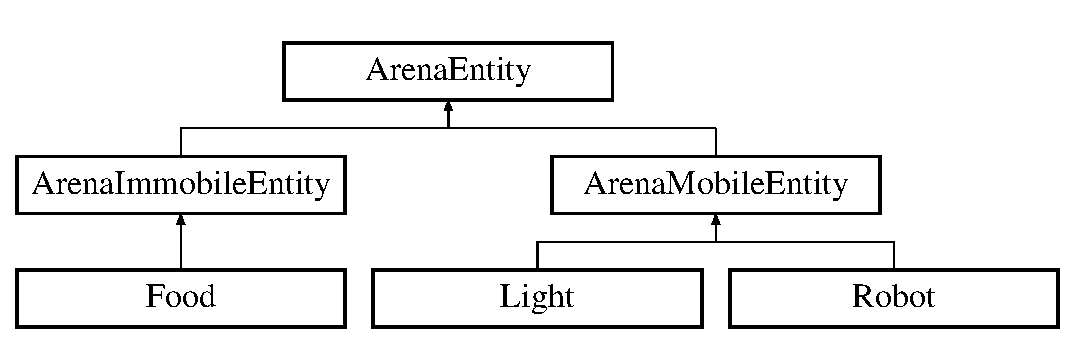
\includegraphics[height=3.000000cm]{class_arena_entity}
\end{center}
\end{figure}
\subsection*{Public Member Functions}
\begin{DoxyCompactItemize}
\item 
\mbox{\Hypertarget{class_arena_entity_a96df749814e89344a6149e4da89b4e44}\label{class_arena_entity_a96df749814e89344a6149e4da89b4e44}} 
\mbox{\hyperlink{class_arena_entity_a96df749814e89344a6149e4da89b4e44}{Arena\+Entity}} ()
\begin{DoxyCompactList}\small\item\em \mbox{\hyperlink{class_arena_entity}{Arena\+Entity}} constructor initialized with default values from \mbox{\hyperlink{params_8h}{params.\+h}}. \end{DoxyCompactList}\item 
\mbox{\Hypertarget{class_arena_entity_aa7af53e5d8830d144ccf2ad07d9140da}\label{class_arena_entity_aa7af53e5d8830d144ccf2ad07d9140da}} 
virtual \mbox{\hyperlink{class_arena_entity_aa7af53e5d8830d144ccf2ad07d9140da}{$\sim$\+Arena\+Entity}} ()=default
\begin{DoxyCompactList}\small\item\em Default destructor -- as defined by compiler. \end{DoxyCompactList}\item 
virtual void \mbox{\hyperlink{class_arena_entity_a203613c40a5cecf47606b2a59adcc3bd}{Timestep\+Update}} (\mbox{\hyperlink{common_8h_a2e3484535ee610c8e19e9859563abe48}{\+\_\+\+\_\+unused}} unsigned int dt)
\begin{DoxyCompactList}\small\item\em Perform whatever updates needed for a particular entity after 1 timestep (updating position, changing color, etc.). \end{DoxyCompactList}\item 
virtual void \mbox{\hyperlink{class_arena_entity_aa9a83946e47cf824ce50325a4599eea8}{Handle\+Collision}} (\mbox{\hyperlink{common_8h_a2e3484535ee610c8e19e9859563abe48}{\+\_\+\+\_\+unused}} Entity\+Type object\+\_\+type, \mbox{\hyperlink{common_8h_a2e3484535ee610c8e19e9859563abe48}{\+\_\+\+\_\+unused}} \mbox{\hyperlink{class_arena_entity}{Arena\+Entity}} $\ast$object)
\begin{DoxyCompactList}\small\item\em handle collisons for both the \mbox{\hyperlink{class_light}{Light}} and the robot, Each using it in a away appropiate to that mobile entity \end{DoxyCompactList}\item 
\mbox{\Hypertarget{class_arena_entity_abaebe6c02659e22c08579d49829c5676}\label{class_arena_entity_abaebe6c02659e22c08579d49829c5676}} 
virtual void \mbox{\hyperlink{class_arena_entity_abaebe6c02659e22c08579d49829c5676}{Reset}} ()
\begin{DoxyCompactList}\small\item\em Reset entity to a newly constructed state. \end{DoxyCompactList}\item 
\mbox{\Hypertarget{class_arena_entity_ad9d597b105a901a79c45cbf704c115d0}\label{class_arena_entity_ad9d597b105a901a79c45cbf704c115d0}} 
\mbox{\hyperlink{struct_pose}{Pose}} \mbox{\hyperlink{class_arena_entity_ad9d597b105a901a79c45cbf704c115d0}{Set\+Pose\+Randomly}} ()
\begin{DoxyCompactList}\small\item\em Randomly place the entity at a spot. \end{DoxyCompactList}\item 
virtual std\+::string \mbox{\hyperlink{class_arena_entity_ad43152003033cf01ad86eeff1990b69a}{get\+\_\+name}} () const =0
\begin{DoxyCompactList}\small\item\em Get the name of the entity for visualization and for debugging. \end{DoxyCompactList}\item 
\mbox{\Hypertarget{class_arena_entity_a9a0efa995da3ed55e92f54357fd2bdae}\label{class_arena_entity_a9a0efa995da3ed55e92f54357fd2bdae}} 
const \mbox{\hyperlink{struct_pose}{Pose}} \& {\bfseries get\+\_\+pose} () const
\item 
\mbox{\Hypertarget{class_arena_entity_a6eb76e5f1b5949314c12cc512d6930ae}\label{class_arena_entity_a6eb76e5f1b5949314c12cc512d6930ae}} 
void {\bfseries set\+\_\+pose} (const \mbox{\hyperlink{struct_pose}{Pose}} \&pose)
\item 
\mbox{\Hypertarget{class_arena_entity_a3136704edf07c24639319abf5c28dac0}\label{class_arena_entity_a3136704edf07c24639319abf5c28dac0}} 
void \mbox{\hyperlink{class_arena_entity_a3136704edf07c24639319abf5c28dac0}{set\+\_\+position}} (const double inx, const double iny)
\begin{DoxyCompactList}\small\item\em Setter method for position within entity pose variable. \end{DoxyCompactList}\item 
\mbox{\Hypertarget{class_arena_entity_ac1cc3c6997bc7a9573128fc5ded9eb72}\label{class_arena_entity_ac1cc3c6997bc7a9573128fc5ded9eb72}} 
void \mbox{\hyperlink{class_arena_entity_ac1cc3c6997bc7a9573128fc5ded9eb72}{set\+\_\+heading}} (const double t)
\begin{DoxyCompactList}\small\item\em Setter method for heading within entity pose variable. \end{DoxyCompactList}\item 
void \mbox{\hyperlink{class_arena_entity_a4c4bd7f5ffb778979303c33cb3bc9986}{Relative\+Change\+Heading}} (const double delta)
\begin{DoxyCompactList}\small\item\em Setter for heading within pose, but change is relative to current value. \end{DoxyCompactList}\item 
\mbox{\Hypertarget{class_arena_entity_a5790a5d45229aa76223a8183ac916323}\label{class_arena_entity_a5790a5d45229aa76223a8183ac916323}} 
const \mbox{\hyperlink{struct_rgb_color}{Rgb\+Color}} \& {\bfseries get\+\_\+color} () const
\item 
\mbox{\Hypertarget{class_arena_entity_a1ac33beda7462ac5c7f4f71a70d3fb10}\label{class_arena_entity_a1ac33beda7462ac5c7f4f71a70d3fb10}} 
void {\bfseries set\+\_\+color} (const \mbox{\hyperlink{struct_rgb_color}{Rgb\+Color}} \&color)
\item 
\mbox{\Hypertarget{class_arena_entity_a42d86d2d952b7f2a861d8a6cb46e661e}\label{class_arena_entity_a42d86d2d952b7f2a861d8a6cb46e661e}} 
double {\bfseries get\+\_\+radius} () const
\item 
\mbox{\Hypertarget{class_arena_entity_a2b0c2512fe53d143442da5e357f71505}\label{class_arena_entity_a2b0c2512fe53d143442da5e357f71505}} 
void {\bfseries set\+\_\+radius} (double radius)
\item 
\mbox{\Hypertarget{class_arena_entity_a19e75df5ce971f48e9a522a343a39fb3}\label{class_arena_entity_a19e75df5ce971f48e9a522a343a39fb3}} 
Entity\+Type {\bfseries get\+\_\+type} () const
\item 
\mbox{\Hypertarget{class_arena_entity_aa65c584906d4c22f61488fab98c3392c}\label{class_arena_entity_aa65c584906d4c22f61488fab98c3392c}} 
void {\bfseries set\+\_\+type} (Entity\+Type et)
\item 
\mbox{\Hypertarget{class_arena_entity_ae50750dfde8118c27835ea8e9db8b7ef}\label{class_arena_entity_ae50750dfde8118c27835ea8e9db8b7ef}} 
int {\bfseries get\+\_\+id} () const
\item 
\mbox{\Hypertarget{class_arena_entity_a67f4c0467d32eec76ee6ed033ff9ed2f}\label{class_arena_entity_a67f4c0467d32eec76ee6ed033ff9ed2f}} 
void {\bfseries set\+\_\+id} (int id)
\item 
\mbox{\Hypertarget{class_arena_entity_a9cfea21220c07502abd084afde49ae65}\label{class_arena_entity_a9cfea21220c07502abd084afde49ae65}} 
bool \mbox{\hyperlink{class_arena_entity_a9cfea21220c07502abd084afde49ae65}{is\+\_\+mobile}} (void)
\begin{DoxyCompactList}\small\item\em Getter method for determining if entity can move or not. \end{DoxyCompactList}\item 
\mbox{\Hypertarget{class_arena_entity_adb5d3089fec5c28cc989e5834fcdaf6c}\label{class_arena_entity_adb5d3089fec5c28cc989e5834fcdaf6c}} 
void \mbox{\hyperlink{class_arena_entity_adb5d3089fec5c28cc989e5834fcdaf6c}{set\+\_\+mobility}} (bool value)
\begin{DoxyCompactList}\small\item\em Setter method for indicating if entity can move or not. \end{DoxyCompactList}\end{DoxyCompactItemize}


\subsection{Detailed Description}
A base class from which all \mbox{\hyperlink{class_arena}{Arena}} entities inherit. 

All entities know how to\+:


\begin{DoxyEnumerate}
\item Update themselves at each timestep (i.\+e. in accordance with current velocity and position).
\item Reset themselves to a newly constructed state. So that the user can click the reset button to restart the game. Alternatively, the game will be reset if the robot has won/lost.
\end{DoxyEnumerate}

Please note that here use the upper-\/left coordinate, which means that the origin point (0.\+0,0.\+0) is at the upper left.

All arena entities are circular. 

\subsection{Member Function Documentation}
\mbox{\Hypertarget{class_arena_entity_ad43152003033cf01ad86eeff1990b69a}\label{class_arena_entity_ad43152003033cf01ad86eeff1990b69a}} 
\index{Arena\+Entity@{Arena\+Entity}!get\+\_\+name@{get\+\_\+name}}
\index{get\+\_\+name@{get\+\_\+name}!Arena\+Entity@{Arena\+Entity}}
\subsubsection{\texorpdfstring{get\+\_\+name()}{get\_name()}}
{\footnotesize\ttfamily virtual std\+::string Arena\+Entity\+::get\+\_\+name (\begin{DoxyParamCaption}{ }\end{DoxyParamCaption}) const\hspace{0.3cm}{\ttfamily [pure virtual]}}



Get the name of the entity for visualization and for debugging. 

\begin{DoxyReturn}{Returns}
Name of the entity. Each entity type hard codes its name (e.\+g. \char`\"{}\+Robot\char`\"{}). 
\end{DoxyReturn}


Implemented in \mbox{\hyperlink{class_robot_a3f77c13705b8f60480d21d8d936dc39e}{Robot}}, \mbox{\hyperlink{class_food_a5c3bcd5109750a15ebb24b8a2a3cdd07}{Food}}, and \mbox{\hyperlink{class_light_a49b2e32cf8173353ac4689fdadbb95d5}{Light}}.

\mbox{\Hypertarget{class_arena_entity_aa9a83946e47cf824ce50325a4599eea8}\label{class_arena_entity_aa9a83946e47cf824ce50325a4599eea8}} 
\index{Arena\+Entity@{Arena\+Entity}!Handle\+Collision@{Handle\+Collision}}
\index{Handle\+Collision@{Handle\+Collision}!Arena\+Entity@{Arena\+Entity}}
\subsubsection{\texorpdfstring{Handle\+Collision()}{HandleCollision()}}
{\footnotesize\ttfamily virtual void Arena\+Entity\+::\+Handle\+Collision (\begin{DoxyParamCaption}\item[{\mbox{\hyperlink{common_8h_a2e3484535ee610c8e19e9859563abe48}{\+\_\+\+\_\+unused}} Entity\+Type}]{object\+\_\+type,  }\item[{\mbox{\hyperlink{common_8h_a2e3484535ee610c8e19e9859563abe48}{\+\_\+\+\_\+unused}} \mbox{\hyperlink{class_arena_entity}{Arena\+Entity}} $\ast$}]{object }\end{DoxyParamCaption})\hspace{0.3cm}{\ttfamily [inline]}, {\ttfamily [virtual]}}



handle collisons for both the \mbox{\hyperlink{class_light}{Light}} and the robot, Each using it in a away appropiate to that mobile entity 


\begin{DoxyParams}[1]{Parameters}
\mbox{\tt in}  & {\em the} & type of the object it collied with. Unused. \\
\hline
\mbox{\tt in}  & {\em the} & actual object it collied with. Unused. \\
\hline
\end{DoxyParams}
\mbox{\Hypertarget{class_arena_entity_a4c4bd7f5ffb778979303c33cb3bc9986}\label{class_arena_entity_a4c4bd7f5ffb778979303c33cb3bc9986}} 
\index{Arena\+Entity@{Arena\+Entity}!Relative\+Change\+Heading@{Relative\+Change\+Heading}}
\index{Relative\+Change\+Heading@{Relative\+Change\+Heading}!Arena\+Entity@{Arena\+Entity}}
\subsubsection{\texorpdfstring{Relative\+Change\+Heading()}{RelativeChangeHeading()}}
{\footnotesize\ttfamily void Arena\+Entity\+::\+Relative\+Change\+Heading (\begin{DoxyParamCaption}\item[{const double}]{delta }\end{DoxyParamCaption})\hspace{0.3cm}{\ttfamily [inline]}}



Setter for heading within pose, but change is relative to current value. 


\begin{DoxyParams}[1]{Parameters}
\mbox{\tt in}  & {\em delta} & by which to modify current heading. Can be positive or negative. \\
\hline
\end{DoxyParams}
\mbox{\Hypertarget{class_arena_entity_a203613c40a5cecf47606b2a59adcc3bd}\label{class_arena_entity_a203613c40a5cecf47606b2a59adcc3bd}} 
\index{Arena\+Entity@{Arena\+Entity}!Timestep\+Update@{Timestep\+Update}}
\index{Timestep\+Update@{Timestep\+Update}!Arena\+Entity@{Arena\+Entity}}
\subsubsection{\texorpdfstring{Timestep\+Update()}{TimestepUpdate()}}
{\footnotesize\ttfamily virtual void Arena\+Entity\+::\+Timestep\+Update (\begin{DoxyParamCaption}\item[{\mbox{\hyperlink{common_8h_a2e3484535ee610c8e19e9859563abe48}{\+\_\+\+\_\+unused}} unsigned int}]{dt }\end{DoxyParamCaption})\hspace{0.3cm}{\ttfamily [inline]}, {\ttfamily [virtual]}}



Perform whatever updates needed for a particular entity after 1 timestep (updating position, changing color, etc.). 


\begin{DoxyParams}[1]{Parameters}
\mbox{\tt in}  & {\em dt} & is time elapsed since the last update. Unused. \\
\hline
\end{DoxyParams}


The documentation for this class was generated from the following file\+:\begin{DoxyCompactItemize}
\item 
src/\mbox{\hyperlink{arena__entity_8h}{arena\+\_\+entity.\+h}}\end{DoxyCompactItemize}

\hypertarget{class_arena_immobile_entity}{}\section{Arena\+Immobile\+Entity Class Reference}
\label{class_arena_immobile_entity}\index{Arena\+Immobile\+Entity@{Arena\+Immobile\+Entity}}


An immobile entity in the \hyperlink{class_arena}{Arena}.  




{\ttfamily \#include $<$arena\+\_\+immobile\+\_\+entity.\+h$>$}

Inheritance diagram for Arena\+Immobile\+Entity\+:\begin{figure}[H]
\begin{center}
\leavevmode
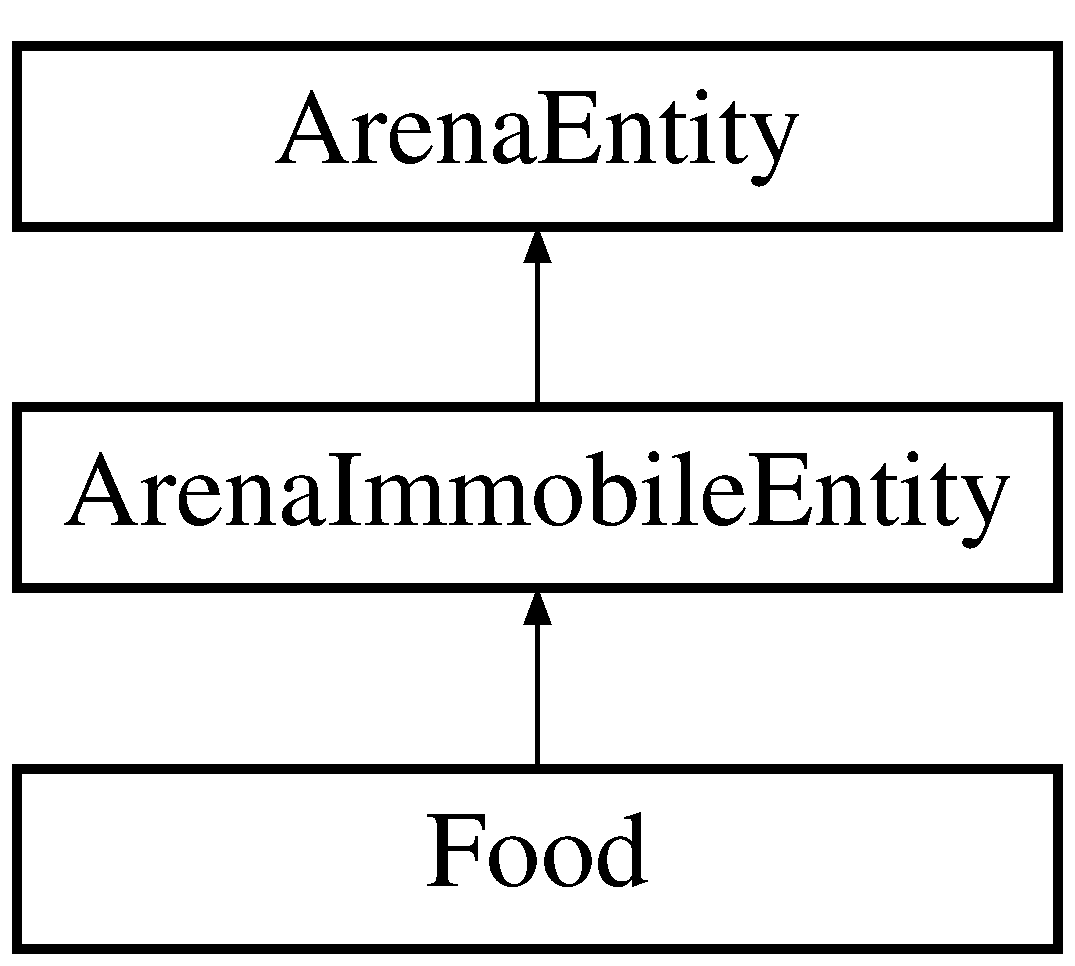
\includegraphics[height=3.000000cm]{class_arena_immobile_entity}
\end{center}
\end{figure}
\subsection*{Public Member Functions}
\begin{DoxyCompactItemize}
\item 
\hyperlink{class_arena_immobile_entity_ac24bb0af97a140d62dd52124489032fd}{Arena\+Immobile\+Entity} ()
\begin{DoxyCompactList}\small\item\em \hyperlink{class_arena_immobile_entity}{Arena\+Immobile\+Entity}\textquotesingle{}s constructor. \end{DoxyCompactList}\end{DoxyCompactItemize}


\subsection{Detailed Description}
An immobile entity in the \hyperlink{class_arena}{Arena}. 

Immobile entities cannot move, and therefore do not need to override the \hyperlink{class_arena_entity_a203613c40a5cecf47606b2a59adcc3bd}{Timestep\+Update()} function. 

\subsection{Constructor \& Destructor Documentation}
\index{Arena\+Immobile\+Entity@{Arena\+Immobile\+Entity}!Arena\+Immobile\+Entity@{Arena\+Immobile\+Entity}}
\index{Arena\+Immobile\+Entity@{Arena\+Immobile\+Entity}!Arena\+Immobile\+Entity@{Arena\+Immobile\+Entity}}
\subsubsection[{\texorpdfstring{Arena\+Immobile\+Entity()}{ArenaImmobileEntity()}}]{\setlength{\rightskip}{0pt plus 5cm}Arena\+Immobile\+Entity\+::\+Arena\+Immobile\+Entity (
\begin{DoxyParamCaption}
{}
\end{DoxyParamCaption}
)\hspace{0.3cm}{\ttfamily [inline]}}\hypertarget{class_arena_immobile_entity_ac24bb0af97a140d62dd52124489032fd}{}\label{class_arena_immobile_entity_ac24bb0af97a140d62dd52124489032fd}


\hyperlink{class_arena_immobile_entity}{Arena\+Immobile\+Entity}\textquotesingle{}s constructor. 


\begin{DoxyParams}{Parameters}
{\em radius} & The radius of the entity (as it is circular). \\
\hline
{\em pos} & The initial position of the entity. \\
\hline
{\em color} & The color of the entity as shown on the screen. \\
\hline
\end{DoxyParams}


The documentation for this class was generated from the following file\+:\begin{DoxyCompactItemize}
\item 
src/\hyperlink{arena__immobile__entity_8h}{arena\+\_\+immobile\+\_\+entity.\+h}\end{DoxyCompactItemize}

\hypertarget{class_arena_mobile_entity}{}\section{Arena\+Mobile\+Entity Class Reference}
\label{class_arena_mobile_entity}\index{Arena\+Mobile\+Entity@{Arena\+Mobile\+Entity}}


A mobile entity in the \hyperlink{class_arena}{Arena}, capable of updating its own position and/or velocity when asked by the simulation.  




{\ttfamily \#include $<$arena\+\_\+mobile\+\_\+entity.\+h$>$}

Inheritance diagram for Arena\+Mobile\+Entity\+:\begin{figure}[H]
\begin{center}
\leavevmode
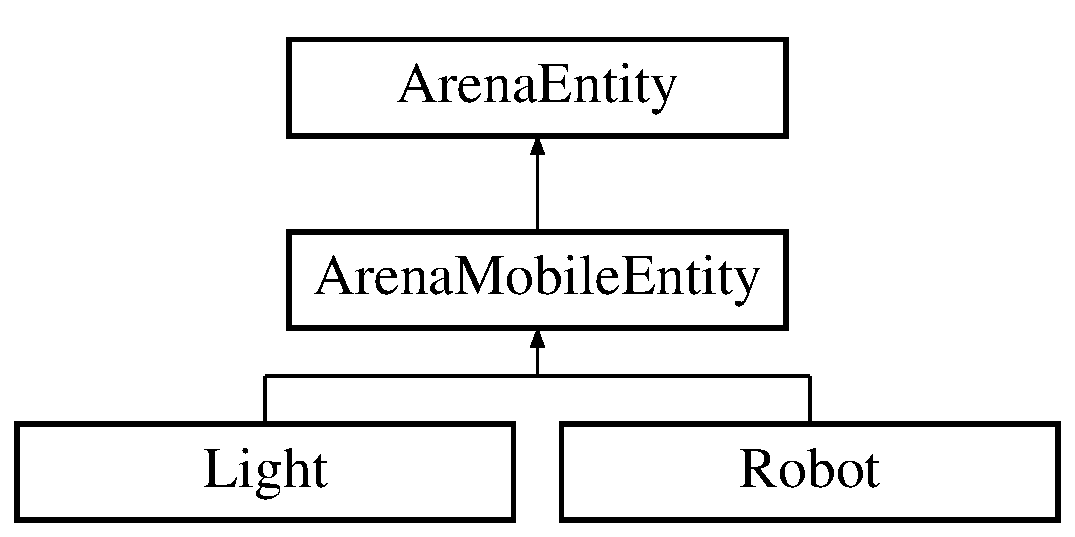
\includegraphics[height=3.000000cm]{class_arena_mobile_entity}
\end{center}
\end{figure}
\subsection*{Public Member Functions}
\begin{DoxyCompactItemize}
\item 
\hyperlink{class_arena_mobile_entity_a6d038ac71d9b149052fc5a0fec4907f9}{Arena\+Mobile\+Entity} ()\hypertarget{class_arena_mobile_entity_a6d038ac71d9b149052fc5a0fec4907f9}{}\label{class_arena_mobile_entity_a6d038ac71d9b149052fc5a0fec4907f9}

\begin{DoxyCompactList}\small\item\em \hyperlink{class_arena_mobile_entity}{Arena\+Mobile\+Entity}\textquotesingle{}s constructor. \end{DoxyCompactList}\item 
{\bfseries Arena\+Mobile\+Entity} (const \hyperlink{class_arena_mobile_entity}{Arena\+Mobile\+Entity} \&other)=delete\hypertarget{class_arena_mobile_entity_ad662f3efc1a56b64ecaf5633e7ff2139}{}\label{class_arena_mobile_entity_ad662f3efc1a56b64ecaf5633e7ff2139}

\item 
\hyperlink{class_arena_mobile_entity}{Arena\+Mobile\+Entity} \& {\bfseries operator=} (const \hyperlink{class_arena_mobile_entity}{Arena\+Mobile\+Entity} \&other)=delete\hypertarget{class_arena_mobile_entity_a34a7f0d094515cafff7611a0f6cf4eee}{}\label{class_arena_mobile_entity_a34a7f0d094515cafff7611a0f6cf4eee}

\item 
virtual double {\bfseries get\+\_\+speed} ()\hypertarget{class_arena_mobile_entity_a2116341414a3ad0449dc03efa6ea500b}{}\label{class_arena_mobile_entity_a2116341414a3ad0449dc03efa6ea500b}

\item 
virtual void {\bfseries set\+\_\+speed} (double sp)\hypertarget{class_arena_mobile_entity_a1a047f4377a9557516a2e1d6d73db849}{}\label{class_arena_mobile_entity_a1a047f4377a9557516a2e1d6d73db849}

\item 
\hyperlink{class_sensor_touch}{Sensor\+Touch} $\ast$ \hyperlink{class_arena_mobile_entity_ae9507f1b0c6bfdfd62afbab8a9a150f7}{get\+\_\+touch\+\_\+sensor} ()\hypertarget{class_arena_mobile_entity_ae9507f1b0c6bfdfd62afbab8a9a150f7}{}\label{class_arena_mobile_entity_ae9507f1b0c6bfdfd62afbab8a9a150f7}

\begin{DoxyCompactList}\small\item\em Get a pointer to the \hyperlink{class_arena_mobile_entity}{Arena\+Mobile\+Entity}\textquotesingle{}s touch sensor. \end{DoxyCompactList}\item 
bool {\bfseries foodon} ()\hypertarget{class_arena_mobile_entity_a1c39e636ebd97600afdaf1bf1df1315f}{}\label{class_arena_mobile_entity_a1c39e636ebd97600afdaf1bf1df1315f}

\item 
void {\bfseries set\+\_\+food\+Btn} (bool fbtn)\hypertarget{class_arena_mobile_entity_ad2dd0b482ed67685585f056f248b4523}{}\label{class_arena_mobile_entity_ad2dd0b482ed67685585f056f248b4523}

\end{DoxyCompactItemize}
\subsection*{Protected Attributes}
\begin{DoxyCompactItemize}
\item 
\hyperlink{class_sensor_touch}{Sensor\+Touch} $\ast$ {\bfseries sensor\+\_\+touch\+\_\+}\hypertarget{class_arena_mobile_entity_a260fd3fba196ee9ab56f9f2ce6ab4a21}{}\label{class_arena_mobile_entity_a260fd3fba196ee9ab56f9f2ce6ab4a21}

\end{DoxyCompactItemize}


\subsection{Detailed Description}
A mobile entity in the \hyperlink{class_arena}{Arena}, capable of updating its own position and/or velocity when asked by the simulation. 

All mobile entities must have a heading angle so that their orientation can be properly drawn by the \hyperlink{class_graphics_arena_viewer}{Graphics\+Arena\+Viewer}.

Since this is also a base class, many of its methods are intuitively {\ttfamily virtual}. 

The documentation for this class was generated from the following file\+:\begin{DoxyCompactItemize}
\item 
src/\hyperlink{arena__mobile__entity_8h}{arena\+\_\+mobile\+\_\+entity.\+h}\end{DoxyCompactItemize}

\hypertarget{class_controller}{}\section{Controller Class Reference}
\label{class_controller}\index{Controller@{Controller}}


\hyperlink{class_controller}{Controller} that mediates \hyperlink{class_arena}{Arena} and \hyperlink{class_graphics_arena_viewer}{Graphics\+Arena\+Viewer} communication.  




{\ttfamily \#include $<$controller.\+h$>$}

\subsection*{Public Member Functions}
\begin{DoxyCompactItemize}
\item 
\hyperlink{class_controller_a95c56822d667e94b031451729ce069a9}{Controller} ()\hypertarget{class_controller_a95c56822d667e94b031451729ce069a9}{}\label{class_controller_a95c56822d667e94b031451729ce069a9}

\begin{DoxyCompactList}\small\item\em \hyperlink{class_controller}{Controller}\textquotesingle{}s constructor that will create \hyperlink{class_arena}{Arena} and Viewer. \end{DoxyCompactList}\item 
void \hyperlink{class_controller_a17abb2cec6c0109e9b2df3cdc082eaad}{Run} ()\hypertarget{class_controller_a17abb2cec6c0109e9b2df3cdc082eaad}{}\label{class_controller_a17abb2cec6c0109e9b2df3cdc082eaad}

\begin{DoxyCompactList}\small\item\em Run launches the graphics and starts the game. \end{DoxyCompactList}\item 
void \hyperlink{class_controller_a6a4a3eaee03f6c4718da3f8293d7e053}{Advance\+Time} (double dt)\hypertarget{class_controller_a6a4a3eaee03f6c4718da3f8293d7e053}{}\label{class_controller_a6a4a3eaee03f6c4718da3f8293d7e053}

\begin{DoxyCompactList}\small\item\em Advance\+Time is communication from the Viewer to advance the simulation. \end{DoxyCompactList}\item 
void \hyperlink{class_controller_a55b8d46984535adb91f40309914e8852}{Accept\+Communication} (Communication com)\hypertarget{class_controller_a55b8d46984535adb91f40309914e8852}{}\label{class_controller_a55b8d46984535adb91f40309914e8852}

\begin{DoxyCompactList}\small\item\em Accept\+Communication from either the viewer or the \hyperlink{class_arena}{Arena}. \end{DoxyCompactList}\item 
Communication \hyperlink{class_controller_ae9b0504ab74cdacc654528b609074adc}{Convert\+Comm} (Communication com)
\begin{DoxyCompactList}\small\item\em Converts the communication from one to send to the other. \end{DoxyCompactList}\item 
void {\bfseries Config\+Arena} (int robotnum, double coward\+\_\+percent, int lightnum, int foodnum, double sensitivity, bool food\+\_\+on\+\_\+)\hypertarget{class_controller_ad1d08bc573c4e2b454134b08a448aea1}{}\label{class_controller_ad1d08bc573c4e2b454134b08a448aea1}

\end{DoxyCompactItemize}


\subsection{Detailed Description}
\hyperlink{class_controller}{Controller} that mediates \hyperlink{class_arena}{Arena} and \hyperlink{class_graphics_arena_viewer}{Graphics\+Arena\+Viewer} communication. 

The \hyperlink{class_controller}{Controller} instantiates the \hyperlink{class_arena}{Arena} and the \hyperlink{class_graphics_arena_viewer}{Graphics\+Arena\+Viewer}. The viewer contains the main loop that keeps it live, but at each update, the viewer sends a message to the controller to update its time.

Other types of communication between \hyperlink{class_arena}{Arena} and Viewer include\+:
\begin{DoxyItemize}
\item keypresses intercepted by the Viewer.
\item Play/\+Pause/\+New Game user input via the Viewer.
\item Game status from arena to the viewer. 
\end{DoxyItemize}

\subsection{Member Function Documentation}
\index{Controller@{Controller}!Convert\+Comm@{Convert\+Comm}}
\index{Convert\+Comm@{Convert\+Comm}!Controller@{Controller}}
\subsubsection[{\texorpdfstring{Convert\+Comm(\+Communication com)}{ConvertComm(Communication com)}}]{\setlength{\rightskip}{0pt plus 5cm}Communication Controller\+::\+Convert\+Comm (
\begin{DoxyParamCaption}
\item[{Communication}]{com}
\end{DoxyParamCaption}
)}\hypertarget{class_controller_ae9b0504ab74cdacc654528b609074adc}{}\label{class_controller_ae9b0504ab74cdacc654528b609074adc}


Converts the communication from one to send to the other. 

Used primarily for testing purposes to insure communication is being correctly received, interpreted, and relayed.

Converts communication from one source to appropriate communication to the other source. For example, the viewer sends a k\+Key\+Up communication, and this translate to a k\+Increase\+Speed communication to \hyperlink{class_arena}{Arena}. \+: Complete the conversion code for all key presses. 

The documentation for this class was generated from the following files\+:\begin{DoxyCompactItemize}
\item 
src/\hyperlink{controller_8h}{controller.\+h}\item 
src/\hyperlink{controller_8cc}{controller.\+cc}\end{DoxyCompactItemize}

\hypertarget{class_entity_factory}{}\section{Entity\+Factory Class Reference}
\label{class_entity_factory}\index{Entity\+Factory@{Entity\+Factory}}


A factory for the instantiation of all types of arena entities.  




{\ttfamily \#include $<$entity\+\_\+factory.\+h$>$}

\subsection*{Public Member Functions}
\begin{DoxyCompactItemize}
\item 
\mbox{\Hypertarget{class_entity_factory_abaf0c4ceaa682e55f69b0ceae230008a}\label{class_entity_factory_abaf0c4ceaa682e55f69b0ceae230008a}} 
\mbox{\hyperlink{class_entity_factory_abaf0c4ceaa682e55f69b0ceae230008a}{Entity\+Factory}} ()
\begin{DoxyCompactList}\small\item\em \mbox{\hyperlink{class_entity_factory}{Entity\+Factory}} constructor. \end{DoxyCompactList}\item 
\mbox{\Hypertarget{class_entity_factory_ae3246f06fa101178803f76582323d4ad}\label{class_entity_factory_ae3246f06fa101178803f76582323d4ad}} 
virtual \mbox{\hyperlink{class_entity_factory_ae3246f06fa101178803f76582323d4ad}{$\sim$\+Entity\+Factory}} ()=default
\begin{DoxyCompactList}\small\item\em Default destructor. \end{DoxyCompactList}\item 
\mbox{\hyperlink{class_arena_entity}{Arena\+Entity}} $\ast$ \mbox{\hyperlink{class_entity_factory_a2a41674ef60c634ef8f886ead99b7b12}{Create\+Entity}} (Entity\+Type etype, Robot\+Type rt=k\+Undefined\+RT)
\begin{DoxyCompactList}\small\item\em Create\+Entity is primary purpose of this class. \end{DoxyCompactList}\end{DoxyCompactItemize}


\subsection{Detailed Description}
A factory for the instantiation of all types of arena entities. 

The factory keeps track of the number of entities of each type and overall. It assigns ID\textquotesingle{}s to the entity when it creates it. The factory randomly places entities, and in doing so, attempts to not have them overlap. 

\subsection{Member Function Documentation}
\mbox{\Hypertarget{class_entity_factory_a2a41674ef60c634ef8f886ead99b7b12}\label{class_entity_factory_a2a41674ef60c634ef8f886ead99b7b12}} 
\index{Entity\+Factory@{Entity\+Factory}!Create\+Entity@{Create\+Entity}}
\index{Create\+Entity@{Create\+Entity}!Entity\+Factory@{Entity\+Factory}}
\subsubsection{\texorpdfstring{Create\+Entity()}{CreateEntity()}}
{\footnotesize\ttfamily \mbox{\hyperlink{class_arena_entity}{Arena\+Entity}} $\ast$ Entity\+Factory\+::\+Create\+Entity (\begin{DoxyParamCaption}\item[{Entity\+Type}]{etype,  }\item[{Robot\+Type}]{rt = {\ttfamily kUndefinedRT} }\end{DoxyParamCaption})}



Create\+Entity is primary purpose of this class. 


\begin{DoxyParams}[1]{Parameters}
\mbox{\tt in}  & {\em etype} & The type to make. \\
\hline
\mbox{\tt out}  & {\em new} & dynamically created entity.\\
\hline
\end{DoxyParams}
Currently, the \mbox{\hyperlink{class_arena}{Arena}} gets the entity and places it in the appropriate data structure. It might be useful to instead have the factory place on the appropriate data structure so that the call to \mbox{\hyperlink{class_arena}{Arena}} is the same regardless of the entity type. 

The documentation for this class was generated from the following files\+:\begin{DoxyCompactItemize}
\item 
src/\mbox{\hyperlink{entity__factory_8h}{entity\+\_\+factory.\+h}}\item 
src/\mbox{\hyperlink{entity__factory_8cc}{entity\+\_\+factory.\+cc}}\end{DoxyCompactItemize}

\hypertarget{class_food}{}\section{Food Class Reference}
\label{class_food}\index{Food@{Food}}


Class representing a immobile \mbox{\hyperlink{class_food}{Food}} within the \mbox{\hyperlink{class_arena}{Arena}}.  




{\ttfamily \#include $<$food.\+h$>$}

Inheritance diagram for Food\+:\begin{figure}[H]
\begin{center}
\leavevmode
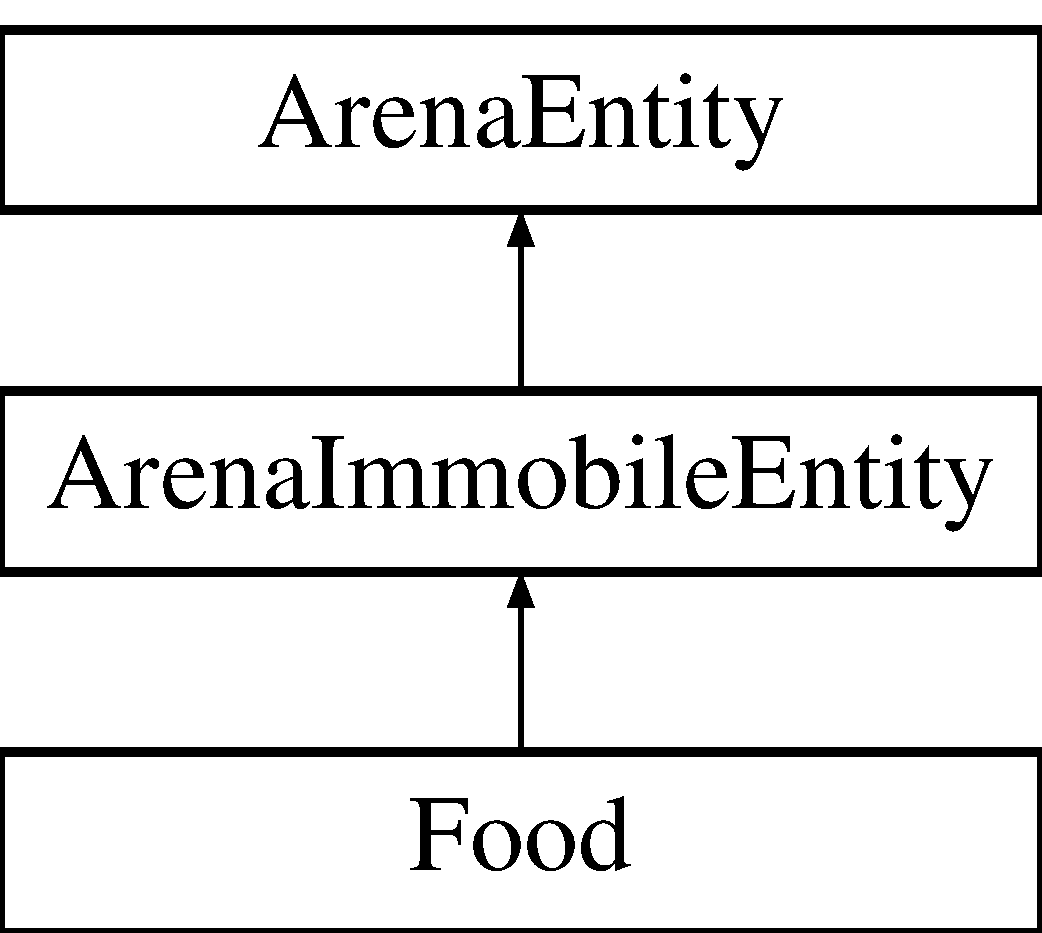
\includegraphics[height=3.000000cm]{class_food}
\end{center}
\end{figure}
\subsection*{Public Member Functions}
\begin{DoxyCompactItemize}
\item 
\mbox{\hyperlink{class_food_a75d4d7f76fd495cc8133302ca9fdc485}{Food}} ()
\begin{DoxyCompactList}\small\item\em Constructor. \end{DoxyCompactList}\item 
\mbox{\Hypertarget{class_food_a1a12bfd50400e04b595c24a512317c1a}\label{class_food_a1a12bfd50400e04b595c24a512317c1a}} 
void \mbox{\hyperlink{class_food_a1a12bfd50400e04b595c24a512317c1a}{Reset}} () override
\begin{DoxyCompactList}\small\item\em Reset the \mbox{\hyperlink{class_food}{Food}} using the initialization parameters received by the constructor. \end{DoxyCompactList}\item 
std\+::string \mbox{\hyperlink{class_food_a5c3bcd5109750a15ebb24b8a2a3cdd07}{get\+\_\+name}} () const override
\begin{DoxyCompactList}\small\item\em Get the name of the \mbox{\hyperlink{class_food}{Food}} for visualization purposes, and to aid in debugging. \end{DoxyCompactList}\end{DoxyCompactItemize}


\subsection{Detailed Description}
Class representing a immobile \mbox{\hyperlink{class_food}{Food}} within the \mbox{\hyperlink{class_arena}{Arena}}. 

\mbox{\hyperlink{class_food}{Food}} have the capability of updating their own position when asked, and also track their own velocity and heading. They have a touch sensor for responding to collision events which is activated/deactivated on collision events. 

\subsection{Constructor \& Destructor Documentation}
\mbox{\Hypertarget{class_food_a75d4d7f76fd495cc8133302ca9fdc485}\label{class_food_a75d4d7f76fd495cc8133302ca9fdc485}} 
\index{Food@{Food}!Food@{Food}}
\index{Food@{Food}!Food@{Food}}
\subsubsection{\texorpdfstring{Food()}{Food()}}
{\footnotesize\ttfamily Food\+::\+Food (\begin{DoxyParamCaption}{ }\end{DoxyParamCaption})}



Constructor. 


\begin{DoxyParams}{Parameters}
{\em params} & A Food\+\_\+params passed down from \mbox{\hyperlink{main_8cc}{main.\+cc}} for the initialization of the \mbox{\hyperlink{class_food}{Food}}. \\
\hline
\end{DoxyParams}


\subsection{Member Function Documentation}
\mbox{\Hypertarget{class_food_a5c3bcd5109750a15ebb24b8a2a3cdd07}\label{class_food_a5c3bcd5109750a15ebb24b8a2a3cdd07}} 
\index{Food@{Food}!get\+\_\+name@{get\+\_\+name}}
\index{get\+\_\+name@{get\+\_\+name}!Food@{Food}}
\subsubsection{\texorpdfstring{get\+\_\+name()}{get\_name()}}
{\footnotesize\ttfamily std\+::string Food\+::get\+\_\+name (\begin{DoxyParamCaption}{ }\end{DoxyParamCaption}) const\hspace{0.3cm}{\ttfamily [inline]}, {\ttfamily [override]}, {\ttfamily [virtual]}}



Get the name of the \mbox{\hyperlink{class_food}{Food}} for visualization purposes, and to aid in debugging. 

\begin{DoxyReturn}{Returns}
Name of the \mbox{\hyperlink{class_food}{Food}}. 
\end{DoxyReturn}


Implements \mbox{\hyperlink{class_arena_entity_ad43152003033cf01ad86eeff1990b69a}{Arena\+Entity}}.



The documentation for this class was generated from the following files\+:\begin{DoxyCompactItemize}
\item 
src/\mbox{\hyperlink{food_8h}{food.\+h}}\item 
src/\mbox{\hyperlink{food_8cc}{food.\+cc}}\end{DoxyCompactItemize}

\hypertarget{class_food_sensor}{}\section{Food\+Sensor Class Reference}
\label{class_food_sensor}\index{Food\+Sensor@{Food\+Sensor}}
Inheritance diagram for Food\+Sensor\+:\begin{figure}[H]
\begin{center}
\leavevmode
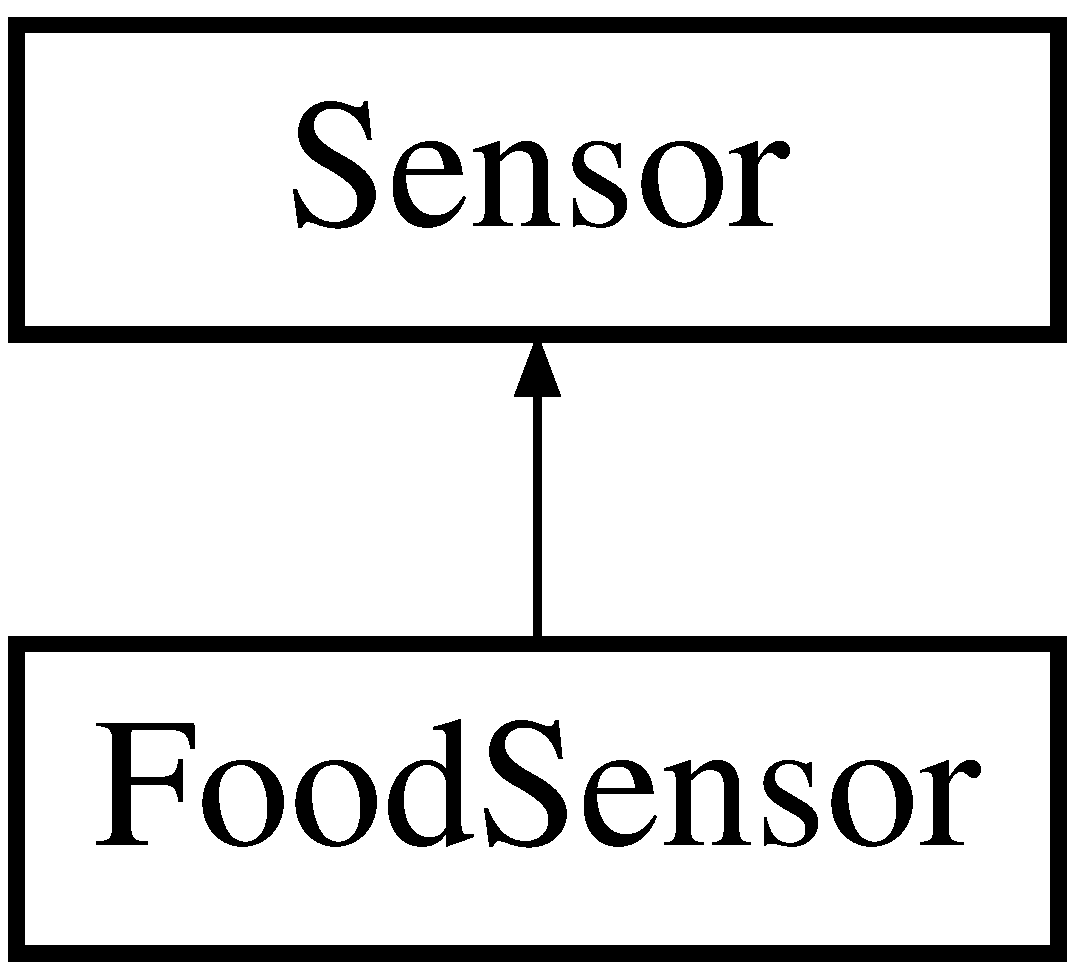
\includegraphics[height=2.000000cm]{class_food_sensor}
\end{center}
\end{figure}
\subsection*{Public Member Functions}
\begin{DoxyCompactItemize}
\item 
\hyperlink{class_food_sensor_a69a35d7061b547ef3140aa03d889b749}{Food\+Sensor} (\hyperlink{class_arena_mobile_entity}{Arena\+Mobile\+Entity} $\ast$ent)\hypertarget{class_food_sensor_a69a35d7061b547ef3140aa03d889b749}{}\label{class_food_sensor_a69a35d7061b547ef3140aa03d889b749}

\begin{DoxyCompactList}\small\item\em food sesnor that inherits from the parent sesnor class \end{DoxyCompactList}\item 
int \hyperlink{class_food_sensor_a76e0a85b68b3fb3983d25c43673f37b7}{Calculate\+Reading} (\hyperlink{class_food}{Food} $\ast$ent)\hypertarget{class_food_sensor_a76e0a85b68b3fb3983d25c43673f37b7}{}\label{class_food_sensor_a76e0a85b68b3fb3983d25c43673f37b7}

\begin{DoxyCompactList}\small\item\em calaculates the reading using the expontial function \end{DoxyCompactList}\item 
void \hyperlink{class_food_sensor_a1b60ca32e66f68f2ca7ddd1d6d709764}{Reset} () override\hypertarget{class_food_sensor_a1b60ca32e66f68f2ca7ddd1d6d709764}{}\label{class_food_sensor_a1b60ca32e66f68f2ca7ddd1d6d709764}

\begin{DoxyCompactList}\small\item\em resets the sensors reading \end{DoxyCompactList}\item 
void \hyperlink{class_food_sensor_a9faf073eb425b425846a54cf502a7702}{update} (std\+::vector$<$ class \hyperlink{class_arena_entity}{Arena\+Entity} $\ast$ $>$ stimili) override\hypertarget{class_food_sensor_a9faf073eb425b425846a54cf502a7702}{}\label{class_food_sensor_a9faf073eb425b425846a54cf502a7702}

\begin{DoxyCompactList}\small\item\em accumalates the reading by calling the Calculate\+Reading for each food in the arena \end{DoxyCompactList}\end{DoxyCompactItemize}
\subsection*{Additional Inherited Members}


The documentation for this class was generated from the following files\+:\begin{DoxyCompactItemize}
\item 
src/\hyperlink{food__sensor_8h}{food\+\_\+sensor.\+h}\item 
src/\hyperlink{food__sensor_8cc}{food\+\_\+sensor.\+cc}\end{DoxyCompactItemize}

\hypertarget{class_graphics_arena_viewer}{}\section{Graphics\+Arena\+Viewer Class Reference}
\label{class_graphics_arena_viewer}\index{Graphics\+Arena\+Viewer@{Graphics\+Arena\+Viewer}}


An application that uses the Min\+Gfx library to open up a window that includes a few buttons for controlling the simulation and can be used to draw circles and other computer graphics.  




{\ttfamily \#include $<$graphics\+\_\+arena\+\_\+viewer.\+h$>$}

Inheritance diagram for Graphics\+Arena\+Viewer\+:\begin{figure}[H]
\begin{center}
\leavevmode
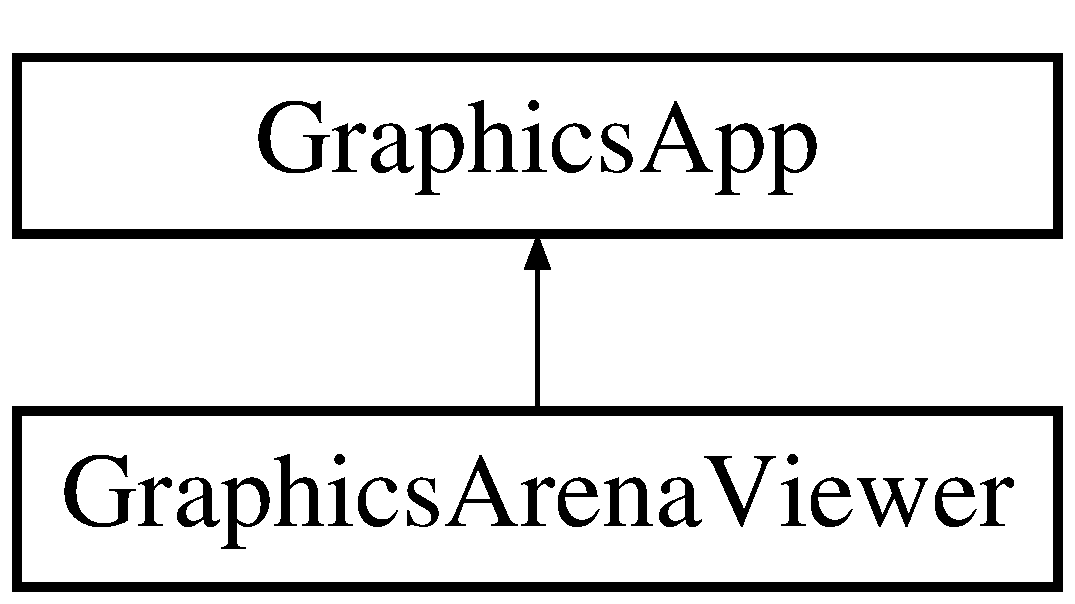
\includegraphics[height=2.000000cm]{class_graphics_arena_viewer}
\end{center}
\end{figure}
\subsection*{Public Member Functions}
\begin{DoxyCompactItemize}
\item 
\hyperlink{class_graphics_arena_viewer_a869510833897508300da65b1eb0c5d09}{Graphics\+Arena\+Viewer} (const struct \hyperlink{structarena__params}{arena\+\_\+params} $\ast$const params, \hyperlink{class_arena}{Arena} $\ast$arena, \hyperlink{class_controller}{Controller} $\ast$controller)
\begin{DoxyCompactList}\small\item\em Constructor. \end{DoxyCompactList}\item 
\hyperlink{class_graphics_arena_viewer_a88cea02aab1550a7f315fbf4f3868109}{$\sim$\+Graphics\+Arena\+Viewer} () override
\begin{DoxyCompactList}\small\item\em Destructor. \end{DoxyCompactList}\item 
void \hyperlink{class_graphics_arena_viewer_aeec66666382aa0312574d70aa58de250}{Update\+Simulation} (double dt) override
\begin{DoxyCompactList}\small\item\em Informs the \hyperlink{class_arena}{Arena} of the new time, so that it can update. \end{DoxyCompactList}\item 
void \hyperlink{class_graphics_arena_viewer_a7cc65fd0e2e8c1f6138608e398c7c887}{On\+Playing\+Btn\+Pressed} ()
\begin{DoxyCompactList}\small\item\em Handle the user pressing the pause button on the G\+UI. \end{DoxyCompactList}\item 
void \hyperlink{class_graphics_arena_viewer_a2f0a3c938191d5becda127e0ddf8bf25}{New\+Game\+Btn\+Pressed} ()
\begin{DoxyCompactList}\small\item\em Handle the user pressing the New game on the G\+UI. \end{DoxyCompactList}\item 
void \hyperlink{class_graphics_arena_viewer_a52f92251a44f82cf7ebf183ece199ceb}{food\+On\+Off\+Btn\+Pressed} ()
\begin{DoxyCompactList}\small\item\em Called each time the mouse moves on the screen within the G\+UI window. \end{DoxyCompactList}\item 
void {\bfseries On\+Mouse\+Move} (\hyperlink{common_8h_a2e3484535ee610c8e19e9859563abe48}{\+\_\+\+\_\+unused} const Point2 \&pos, \hyperlink{common_8h_a2e3484535ee610c8e19e9859563abe48}{\+\_\+\+\_\+unused} const Vector2 \&delta) override\hypertarget{class_graphics_arena_viewer_a74b5c524369a62ba419c89677c646d9e}{}\label{class_graphics_arena_viewer_a74b5c524369a62ba419c89677c646d9e}

\item 
void \hyperlink{class_graphics_arena_viewer_adf2fb01c3ca8b1774f031d68616b288c}{On\+Left\+Mouse\+Down} (\hyperlink{common_8h_a2e3484535ee610c8e19e9859563abe48}{\+\_\+\+\_\+unused} const Point2 \&pos) override
\begin{DoxyCompactList}\small\item\em Called each time the left mouse button is clicked. \end{DoxyCompactList}\item 
void \hyperlink{class_graphics_arena_viewer_abe4f11ab9bfb6055280ddf2b671d7032}{On\+Left\+Mouse\+Up} (\hyperlink{common_8h_a2e3484535ee610c8e19e9859563abe48}{\+\_\+\+\_\+unused} const Point2 \&pos) override
\begin{DoxyCompactList}\small\item\em Called each time the left mouse button is released. \end{DoxyCompactList}\item 
void \hyperlink{class_graphics_arena_viewer_a178a9f09ff241d4dc032b6d0998cc9c6}{On\+Right\+Mouse\+Down} (\hyperlink{common_8h_a2e3484535ee610c8e19e9859563abe48}{\+\_\+\+\_\+unused} const Point2 \&pos) override
\begin{DoxyCompactList}\small\item\em Called each time the right mouse button is clicked. \end{DoxyCompactList}\item 
void \hyperlink{class_graphics_arena_viewer_a5dfa16dca83575e253b6d3ea344f8746}{On\+Right\+Mouse\+Up} (\hyperlink{common_8h_a2e3484535ee610c8e19e9859563abe48}{\+\_\+\+\_\+unused} const Point2 \&pos) override
\begin{DoxyCompactList}\small\item\em Called each time the right mouse button is released. \end{DoxyCompactList}\item 
void \hyperlink{class_graphics_arena_viewer_ab0001d4a3ebde2b1f5b4cb7770824726}{On\+Key\+Down} (\hyperlink{common_8h_a2e3484535ee610c8e19e9859563abe48}{\+\_\+\+\_\+unused} const char $\ast$c, \hyperlink{common_8h_a2e3484535ee610c8e19e9859563abe48}{\+\_\+\+\_\+unused} int modifiers) override
\begin{DoxyCompactList}\small\item\em Called each time a character key is pressed. \end{DoxyCompactList}\item 
void \hyperlink{class_graphics_arena_viewer_ac3e749f6a75bdd5b32d23c9c8913f9d8}{On\+Key\+Up} (\hyperlink{common_8h_a2e3484535ee610c8e19e9859563abe48}{\+\_\+\+\_\+unused} const char $\ast$c, \hyperlink{common_8h_a2e3484535ee610c8e19e9859563abe48}{\+\_\+\+\_\+unused} int modifiers) override
\begin{DoxyCompactList}\small\item\em Called each time a character key is released. \end{DoxyCompactList}\item 
void \hyperlink{class_graphics_arena_viewer_ab6ed6287ddf72f43f605482ce77b01a2}{On\+Special\+Key\+Down} (int key, \hyperlink{common_8h_a2e3484535ee610c8e19e9859563abe48}{\+\_\+\+\_\+unused} int scancode, \hyperlink{common_8h_a2e3484535ee610c8e19e9859563abe48}{\+\_\+\+\_\+unused} int modifiers) override
\begin{DoxyCompactList}\small\item\em Called each time a special (non-\/alphabetic) key is pressed. \end{DoxyCompactList}\item 
void \hyperlink{class_graphics_arena_viewer_a086e2e29e1a5745a8ee4f12996897b22}{On\+Special\+Key\+Up} (\hyperlink{common_8h_a2e3484535ee610c8e19e9859563abe48}{\+\_\+\+\_\+unused} int key, \hyperlink{common_8h_a2e3484535ee610c8e19e9859563abe48}{\+\_\+\+\_\+unused} int scancode, \hyperlink{common_8h_a2e3484535ee610c8e19e9859563abe48}{\+\_\+\+\_\+unused} int modifiers) override
\begin{DoxyCompactList}\small\item\em Called each time a special (non-\/alphabetic) key is released. \end{DoxyCompactList}\item 
void \hyperlink{class_graphics_arena_viewer_a7d59755e3f7674f382127fe135492eeb}{Draw\+Using\+Nano\+VG} (N\+V\+Gcontext $\ast$ctx) override
\begin{DoxyCompactList}\small\item\em Draw the \hyperlink{class_arena}{Arena} with all of its entities using {\ttfamily nanogui}. \end{DoxyCompactList}\item 
void \hyperlink{class_graphics_arena_viewer_af894508bfa039199c6ff7f1b5a7da158}{Draw\+Using\+Open\+GL} () override\hypertarget{class_graphics_arena_viewer_af894508bfa039199c6ff7f1b5a7da158}{}\label{class_graphics_arena_viewer_af894508bfa039199c6ff7f1b5a7da158}

\begin{DoxyCompactList}\small\item\em Draw using {\ttfamily Open\+GL}. This method is unimplemented, as currently we are doing all drawing with {\ttfamily nanovg} in this application, so it is empty. \end{DoxyCompactList}\item 
\hyperlink{class_graphics_arena_viewer}{Graphics\+Arena\+Viewer} \& \hyperlink{class_graphics_arena_viewer_a289278f7b338fc60f983827d21b159ff}{operator=} (const \hyperlink{class_graphics_arena_viewer}{Graphics\+Arena\+Viewer} \&other)=delete\hypertarget{class_graphics_arena_viewer_a289278f7b338fc60f983827d21b159ff}{}\label{class_graphics_arena_viewer_a289278f7b338fc60f983827d21b159ff}

\begin{DoxyCompactList}\small\item\em Under certain circumstance, the compiler requires that the assignment operator is not defined. This {\ttfamily deletes} the default assignment operator. \end{DoxyCompactList}\item 
\hyperlink{class_graphics_arena_viewer_afa70b72e0769db0f3f41fe37bc540621}{Graphics\+Arena\+Viewer} (const \hyperlink{class_graphics_arena_viewer}{Graphics\+Arena\+Viewer} \&other)=delete\hypertarget{class_graphics_arena_viewer_afa70b72e0769db0f3f41fe37bc540621}{}\label{class_graphics_arena_viewer_afa70b72e0769db0f3f41fe37bc540621}

\begin{DoxyCompactList}\small\item\em Under certain circumstance, the compiler requires that the copy constructor is not defined. This {\ttfamily deletes} the default copy constructor. \end{DoxyCompactList}\end{DoxyCompactItemize}


\subsection{Detailed Description}
An application that uses the Min\+Gfx library to open up a window that includes a few buttons for controlling the simulation and can be used to draw circles and other computer graphics. 

After constructing a new \hyperlink{class_graphics_arena_viewer}{Graphics\+Arena\+Viewer}, call Run to start and run the application. Run will not return until the application window is closed. Example\+:


\begin{DoxyCode}
\textcolor{keywordtype}{int} main(\textcolor{keywordtype}{int} argc, \textcolor{keywordtype}{char} **argv) \{
    RobotViewer *app = \textcolor{keyword}{new} RobotViewer();
    app->Run();
    \textcolor{keywordflow}{return} 0;
\}
\end{DoxyCode}


While the window is open Update\+Simulation will be called repeatedly, once per frame. Fill this in to update your simulation or perform any other processing that should happen over time as the simulation progresses.

Fill in the {\ttfamily On$\ast$()} methods as desired to respond to user input events.

Fill in the {\ttfamily Draw$\ast$()} methods to draw graphics on the screen using either the {\ttfamily nanovg} library or raw {\ttfamily Open\+GL}. 

\subsection{Constructor \& Destructor Documentation}
\index{Graphics\+Arena\+Viewer@{Graphics\+Arena\+Viewer}!Graphics\+Arena\+Viewer@{Graphics\+Arena\+Viewer}}
\index{Graphics\+Arena\+Viewer@{Graphics\+Arena\+Viewer}!Graphics\+Arena\+Viewer@{Graphics\+Arena\+Viewer}}
\subsubsection[{\texorpdfstring{Graphics\+Arena\+Viewer(const struct arena\+\_\+params $\ast$const params, Arena $\ast$arena, Controller $\ast$controller)}{GraphicsArenaViewer(const struct arena_params *const params, Arena *arena, Controller *controller)}}]{\setlength{\rightskip}{0pt plus 5cm}Graphics\+Arena\+Viewer\+::\+Graphics\+Arena\+Viewer (
\begin{DoxyParamCaption}
\item[{const struct {\bf arena\+\_\+params} $\ast$const}]{params, }
\item[{{\bf Arena} $\ast$}]{arena, }
\item[{{\bf Controller} $\ast$}]{controller}
\end{DoxyParamCaption}
)\hspace{0.3cm}{\ttfamily [explicit]}}\hypertarget{class_graphics_arena_viewer_a869510833897508300da65b1eb0c5d09}{}\label{class_graphics_arena_viewer_a869510833897508300da65b1eb0c5d09}


Constructor. 


\begin{DoxyParams}{Parameters}
{\em params} & A \hyperlink{structarena__params}{arena\+\_\+params} passed down from \hyperlink{main_8cc}{main.\+cc} for the initialization of the \hyperlink{class_arena}{Arena} and the entities therein. \\
\hline
\end{DoxyParams}
\index{Graphics\+Arena\+Viewer@{Graphics\+Arena\+Viewer}!````~Graphics\+Arena\+Viewer@{$\sim$\+Graphics\+Arena\+Viewer}}
\index{````~Graphics\+Arena\+Viewer@{$\sim$\+Graphics\+Arena\+Viewer}!Graphics\+Arena\+Viewer@{Graphics\+Arena\+Viewer}}
\subsubsection[{\texorpdfstring{$\sim$\+Graphics\+Arena\+Viewer() override}{~GraphicsArenaViewer() override}}]{\setlength{\rightskip}{0pt plus 5cm}Graphics\+Arena\+Viewer\+::$\sim$\+Graphics\+Arena\+Viewer (
\begin{DoxyParamCaption}
{}
\end{DoxyParamCaption}
)\hspace{0.3cm}{\ttfamily [inline]}, {\ttfamily [override]}}\hypertarget{class_graphics_arena_viewer_a88cea02aab1550a7f315fbf4f3868109}{}\label{class_graphics_arena_viewer_a88cea02aab1550a7f315fbf4f3868109}


Destructor. 

{\ttfamily delete} the contained \hyperlink{class_arena}{Arena}. 

\subsection{Member Function Documentation}
\index{Graphics\+Arena\+Viewer@{Graphics\+Arena\+Viewer}!Draw\+Using\+Nano\+VG@{Draw\+Using\+Nano\+VG}}
\index{Draw\+Using\+Nano\+VG@{Draw\+Using\+Nano\+VG}!Graphics\+Arena\+Viewer@{Graphics\+Arena\+Viewer}}
\subsubsection[{\texorpdfstring{Draw\+Using\+Nano\+V\+G(\+N\+V\+Gcontext $\ast$ctx) override}{DrawUsingNanoVG(NVGcontext *ctx) override}}]{\setlength{\rightskip}{0pt plus 5cm}void Graphics\+Arena\+Viewer\+::\+Draw\+Using\+Nano\+VG (
\begin{DoxyParamCaption}
\item[{N\+V\+Gcontext $\ast$}]{ctx}
\end{DoxyParamCaption}
)\hspace{0.3cm}{\ttfamily [override]}}\hypertarget{class_graphics_arena_viewer_a7d59755e3f7674f382127fe135492eeb}{}\label{class_graphics_arena_viewer_a7d59755e3f7674f382127fe135492eeb}


Draw the \hyperlink{class_arena}{Arena} with all of its entities using {\ttfamily nanogui}. 

This is the primary driver for drawing all entities in the \hyperlink{class_arena}{Arena}. It is called at each iteration of {\ttfamily nanogui\+::mainloop()}.


\begin{DoxyParams}[1]{Parameters}
\mbox{\tt in}  & {\em ctx} & Context for nanogui. \\
\hline
\end{DoxyParams}
\index{Graphics\+Arena\+Viewer@{Graphics\+Arena\+Viewer}!food\+On\+Off\+Btn\+Pressed@{food\+On\+Off\+Btn\+Pressed}}
\index{food\+On\+Off\+Btn\+Pressed@{food\+On\+Off\+Btn\+Pressed}!Graphics\+Arena\+Viewer@{Graphics\+Arena\+Viewer}}
\subsubsection[{\texorpdfstring{food\+On\+Off\+Btn\+Pressed()}{foodOnOffBtnPressed()}}]{\setlength{\rightskip}{0pt plus 5cm}void Graphics\+Arena\+Viewer\+::food\+On\+Off\+Btn\+Pressed (
\begin{DoxyParamCaption}
{}
\end{DoxyParamCaption}
)}\hypertarget{class_graphics_arena_viewer_a52f92251a44f82cf7ebf183ece199ceb}{}\label{class_graphics_arena_viewer_a52f92251a44f82cf7ebf183ece199ceb}


Called each time the mouse moves on the screen within the G\+UI window. 

Origin is at the lower left of the window. This function is a stub.


\begin{DoxyParams}[1]{Parameters}
\mbox{\tt in}  & {\em pos} & The position of the release. \\
\hline
\mbox{\tt in}  & {\em delta} & How far the mouse has moved. \\
\hline
\end{DoxyParams}
\index{Graphics\+Arena\+Viewer@{Graphics\+Arena\+Viewer}!New\+Game\+Btn\+Pressed@{New\+Game\+Btn\+Pressed}}
\index{New\+Game\+Btn\+Pressed@{New\+Game\+Btn\+Pressed}!Graphics\+Arena\+Viewer@{Graphics\+Arena\+Viewer}}
\subsubsection[{\texorpdfstring{New\+Game\+Btn\+Pressed()}{NewGameBtnPressed()}}]{\setlength{\rightskip}{0pt plus 5cm}void Graphics\+Arena\+Viewer\+::\+New\+Game\+Btn\+Pressed (
\begin{DoxyParamCaption}
{}
\end{DoxyParamCaption}
)}\hypertarget{class_graphics_arena_viewer_a2f0a3c938191d5becda127e0ddf8bf25}{}\label{class_graphics_arena_viewer_a2f0a3c938191d5becda127e0ddf8bf25}


Handle the user pressing the New game on the G\+UI. 

This will freeze the graphics--no update, until the play button is pressed again and the arena is reset. \index{Graphics\+Arena\+Viewer@{Graphics\+Arena\+Viewer}!On\+Key\+Down@{On\+Key\+Down}}
\index{On\+Key\+Down@{On\+Key\+Down}!Graphics\+Arena\+Viewer@{Graphics\+Arena\+Viewer}}
\subsubsection[{\texorpdfstring{On\+Key\+Down(\+\_\+\+\_\+unused const char $\ast$c, \+\_\+\+\_\+unused int modifiers) override}{OnKeyDown(__unused const char *c, __unused int modifiers) override}}]{\setlength{\rightskip}{0pt plus 5cm}void Graphics\+Arena\+Viewer\+::\+On\+Key\+Down (
\begin{DoxyParamCaption}
\item[{{\bf \+\_\+\+\_\+unused} const char $\ast$}]{c, }
\item[{{\bf \+\_\+\+\_\+unused} int}]{modifiers}
\end{DoxyParamCaption}
)\hspace{0.3cm}{\ttfamily [inline]}, {\ttfamily [override]}}\hypertarget{class_graphics_arena_viewer_ab0001d4a3ebde2b1f5b4cb7770824726}{}\label{class_graphics_arena_viewer_ab0001d4a3ebde2b1f5b4cb7770824726}


Called each time a character key is pressed. 


\begin{DoxyParams}[1]{Parameters}
\mbox{\tt in}  & {\em c} & Character representing a key that was pressed. \\
\hline
\mbox{\tt in}  & {\em modifiers} & Any modifier keys that were also pressed. \\
\hline
\end{DoxyParams}
\index{Graphics\+Arena\+Viewer@{Graphics\+Arena\+Viewer}!On\+Key\+Up@{On\+Key\+Up}}
\index{On\+Key\+Up@{On\+Key\+Up}!Graphics\+Arena\+Viewer@{Graphics\+Arena\+Viewer}}
\subsubsection[{\texorpdfstring{On\+Key\+Up(\+\_\+\+\_\+unused const char $\ast$c, \+\_\+\+\_\+unused int modifiers) override}{OnKeyUp(__unused const char *c, __unused int modifiers) override}}]{\setlength{\rightskip}{0pt plus 5cm}void Graphics\+Arena\+Viewer\+::\+On\+Key\+Up (
\begin{DoxyParamCaption}
\item[{{\bf \+\_\+\+\_\+unused} const char $\ast$}]{c, }
\item[{{\bf \+\_\+\+\_\+unused} int}]{modifiers}
\end{DoxyParamCaption}
)\hspace{0.3cm}{\ttfamily [inline]}, {\ttfamily [override]}}\hypertarget{class_graphics_arena_viewer_ac3e749f6a75bdd5b32d23c9c8913f9d8}{}\label{class_graphics_arena_viewer_ac3e749f6a75bdd5b32d23c9c8913f9d8}


Called each time a character key is released. 


\begin{DoxyParams}[1]{Parameters}
\mbox{\tt in}  & {\em c} & Character representing a key that was released. \\
\hline
\mbox{\tt in}  & {\em modifiers} & Any modifier keys that were held with the key. \\
\hline
\end{DoxyParams}
\index{Graphics\+Arena\+Viewer@{Graphics\+Arena\+Viewer}!On\+Left\+Mouse\+Down@{On\+Left\+Mouse\+Down}}
\index{On\+Left\+Mouse\+Down@{On\+Left\+Mouse\+Down}!Graphics\+Arena\+Viewer@{Graphics\+Arena\+Viewer}}
\subsubsection[{\texorpdfstring{On\+Left\+Mouse\+Down(\+\_\+\+\_\+unused const Point2 \&pos) override}{OnLeftMouseDown(__unused const Point2 &pos) override}}]{\setlength{\rightskip}{0pt plus 5cm}void Graphics\+Arena\+Viewer\+::\+On\+Left\+Mouse\+Down (
\begin{DoxyParamCaption}
\item[{{\bf \+\_\+\+\_\+unused} const Point2 \&}]{pos}
\end{DoxyParamCaption}
)\hspace{0.3cm}{\ttfamily [inline]}, {\ttfamily [override]}}\hypertarget{class_graphics_arena_viewer_adf2fb01c3ca8b1774f031d68616b288c}{}\label{class_graphics_arena_viewer_adf2fb01c3ca8b1774f031d68616b288c}


Called each time the left mouse button is clicked. 

Origin is at the lower left of the window. This function is a stub.


\begin{DoxyParams}[1]{Parameters}
\mbox{\tt in}  & {\em pos} & The position of the release. \\
\hline
\end{DoxyParams}
\index{Graphics\+Arena\+Viewer@{Graphics\+Arena\+Viewer}!On\+Left\+Mouse\+Up@{On\+Left\+Mouse\+Up}}
\index{On\+Left\+Mouse\+Up@{On\+Left\+Mouse\+Up}!Graphics\+Arena\+Viewer@{Graphics\+Arena\+Viewer}}
\subsubsection[{\texorpdfstring{On\+Left\+Mouse\+Up(\+\_\+\+\_\+unused const Point2 \&pos) override}{OnLeftMouseUp(__unused const Point2 &pos) override}}]{\setlength{\rightskip}{0pt plus 5cm}void Graphics\+Arena\+Viewer\+::\+On\+Left\+Mouse\+Up (
\begin{DoxyParamCaption}
\item[{{\bf \+\_\+\+\_\+unused} const Point2 \&}]{pos}
\end{DoxyParamCaption}
)\hspace{0.3cm}{\ttfamily [inline]}, {\ttfamily [override]}}\hypertarget{class_graphics_arena_viewer_abe4f11ab9bfb6055280ddf2b671d7032}{}\label{class_graphics_arena_viewer_abe4f11ab9bfb6055280ddf2b671d7032}


Called each time the left mouse button is released. 

Origin is at the lower left of the window. This function is a stub.


\begin{DoxyParams}[1]{Parameters}
\mbox{\tt in}  & {\em pos} & The position of the release. \\
\hline
\end{DoxyParams}
\index{Graphics\+Arena\+Viewer@{Graphics\+Arena\+Viewer}!On\+Playing\+Btn\+Pressed@{On\+Playing\+Btn\+Pressed}}
\index{On\+Playing\+Btn\+Pressed@{On\+Playing\+Btn\+Pressed}!Graphics\+Arena\+Viewer@{Graphics\+Arena\+Viewer}}
\subsubsection[{\texorpdfstring{On\+Playing\+Btn\+Pressed()}{OnPlayingBtnPressed()}}]{\setlength{\rightskip}{0pt plus 5cm}void Graphics\+Arena\+Viewer\+::\+On\+Playing\+Btn\+Pressed (
\begin{DoxyParamCaption}
{}
\end{DoxyParamCaption}
)}\hypertarget{class_graphics_arena_viewer_a7cc65fd0e2e8c1f6138608e398c7c887}{}\label{class_graphics_arena_viewer_a7cc65fd0e2e8c1f6138608e398c7c887}


Handle the user pressing the pause button on the G\+UI. 

This will freeze the graphics--no update, until the pause button is pressed again. \index{Graphics\+Arena\+Viewer@{Graphics\+Arena\+Viewer}!On\+Right\+Mouse\+Down@{On\+Right\+Mouse\+Down}}
\index{On\+Right\+Mouse\+Down@{On\+Right\+Mouse\+Down}!Graphics\+Arena\+Viewer@{Graphics\+Arena\+Viewer}}
\subsubsection[{\texorpdfstring{On\+Right\+Mouse\+Down(\+\_\+\+\_\+unused const Point2 \&pos) override}{OnRightMouseDown(__unused const Point2 &pos) override}}]{\setlength{\rightskip}{0pt plus 5cm}void Graphics\+Arena\+Viewer\+::\+On\+Right\+Mouse\+Down (
\begin{DoxyParamCaption}
\item[{{\bf \+\_\+\+\_\+unused} const Point2 \&}]{pos}
\end{DoxyParamCaption}
)\hspace{0.3cm}{\ttfamily [inline]}, {\ttfamily [override]}}\hypertarget{class_graphics_arena_viewer_a178a9f09ff241d4dc032b6d0998cc9c6}{}\label{class_graphics_arena_viewer_a178a9f09ff241d4dc032b6d0998cc9c6}


Called each time the right mouse button is clicked. 

Origin is at the lower left of the window. This function is a stub.


\begin{DoxyParams}[1]{Parameters}
\mbox{\tt in}  & {\em pos} & The position of the release. \\
\hline
\end{DoxyParams}
\index{Graphics\+Arena\+Viewer@{Graphics\+Arena\+Viewer}!On\+Right\+Mouse\+Up@{On\+Right\+Mouse\+Up}}
\index{On\+Right\+Mouse\+Up@{On\+Right\+Mouse\+Up}!Graphics\+Arena\+Viewer@{Graphics\+Arena\+Viewer}}
\subsubsection[{\texorpdfstring{On\+Right\+Mouse\+Up(\+\_\+\+\_\+unused const Point2 \&pos) override}{OnRightMouseUp(__unused const Point2 &pos) override}}]{\setlength{\rightskip}{0pt plus 5cm}void Graphics\+Arena\+Viewer\+::\+On\+Right\+Mouse\+Up (
\begin{DoxyParamCaption}
\item[{{\bf \+\_\+\+\_\+unused} const Point2 \&}]{pos}
\end{DoxyParamCaption}
)\hspace{0.3cm}{\ttfamily [inline]}, {\ttfamily [override]}}\hypertarget{class_graphics_arena_viewer_a5dfa16dca83575e253b6d3ea344f8746}{}\label{class_graphics_arena_viewer_a5dfa16dca83575e253b6d3ea344f8746}


Called each time the right mouse button is released. 

Origin is at the lower left of the window. This function is a stub.


\begin{DoxyParams}[1]{Parameters}
\mbox{\tt in}  & {\em pos} & The position of the release. \\
\hline
\end{DoxyParams}
\index{Graphics\+Arena\+Viewer@{Graphics\+Arena\+Viewer}!On\+Special\+Key\+Down@{On\+Special\+Key\+Down}}
\index{On\+Special\+Key\+Down@{On\+Special\+Key\+Down}!Graphics\+Arena\+Viewer@{Graphics\+Arena\+Viewer}}
\subsubsection[{\texorpdfstring{On\+Special\+Key\+Down(int key, \+\_\+\+\_\+unused int scancode, \+\_\+\+\_\+unused int modifiers) override}{OnSpecialKeyDown(int key, __unused int scancode, __unused int modifiers) override}}]{\setlength{\rightskip}{0pt plus 5cm}void Graphics\+Arena\+Viewer\+::\+On\+Special\+Key\+Down (
\begin{DoxyParamCaption}
\item[{int}]{key, }
\item[{{\bf \+\_\+\+\_\+unused} int}]{scancode, }
\item[{{\bf \+\_\+\+\_\+unused} int}]{modifiers}
\end{DoxyParamCaption}
)\hspace{0.3cm}{\ttfamily [override]}}\hypertarget{class_graphics_arena_viewer_ab6ed6287ddf72f43f605482ce77b01a2}{}\label{class_graphics_arena_viewer_ab6ed6287ddf72f43f605482ce77b01a2}


Called each time a special (non-\/alphabetic) key is pressed. 


\begin{DoxyParams}[1]{Parameters}
\mbox{\tt in}  & {\em key} & The key that was pressed. \\
\hline
\mbox{\tt in}  & {\em scancode} & The scancode corresponding to the key. \\
\hline
\mbox{\tt in}  & {\em modifiers} & Any modifier keys that were also pressed. \\
\hline
\end{DoxyParams}
\index{Graphics\+Arena\+Viewer@{Graphics\+Arena\+Viewer}!On\+Special\+Key\+Up@{On\+Special\+Key\+Up}}
\index{On\+Special\+Key\+Up@{On\+Special\+Key\+Up}!Graphics\+Arena\+Viewer@{Graphics\+Arena\+Viewer}}
\subsubsection[{\texorpdfstring{On\+Special\+Key\+Up(\+\_\+\+\_\+unused int key, \+\_\+\+\_\+unused int scancode, \+\_\+\+\_\+unused int modifiers) override}{OnSpecialKeyUp(__unused int key, __unused int scancode, __unused int modifiers) override}}]{\setlength{\rightskip}{0pt plus 5cm}void Graphics\+Arena\+Viewer\+::\+On\+Special\+Key\+Up (
\begin{DoxyParamCaption}
\item[{{\bf \+\_\+\+\_\+unused} int}]{key, }
\item[{{\bf \+\_\+\+\_\+unused} int}]{scancode, }
\item[{{\bf \+\_\+\+\_\+unused} int}]{modifiers}
\end{DoxyParamCaption}
)\hspace{0.3cm}{\ttfamily [inline]}, {\ttfamily [override]}}\hypertarget{class_graphics_arena_viewer_a086e2e29e1a5745a8ee4f12996897b22}{}\label{class_graphics_arena_viewer_a086e2e29e1a5745a8ee4f12996897b22}


Called each time a special (non-\/alphabetic) key is released. 


\begin{DoxyParams}[1]{Parameters}
\mbox{\tt in}  & {\em key} & The key that was released. \\
\hline
\mbox{\tt in}  & {\em scancode} & The scancode corresponding to the key. \\
\hline
\mbox{\tt in}  & {\em modifiers} & Any modifier keys that were also pressed. \\
\hline
\end{DoxyParams}
\index{Graphics\+Arena\+Viewer@{Graphics\+Arena\+Viewer}!Update\+Simulation@{Update\+Simulation}}
\index{Update\+Simulation@{Update\+Simulation}!Graphics\+Arena\+Viewer@{Graphics\+Arena\+Viewer}}
\subsubsection[{\texorpdfstring{Update\+Simulation(double dt) override}{UpdateSimulation(double dt) override}}]{\setlength{\rightskip}{0pt plus 5cm}void Graphics\+Arena\+Viewer\+::\+Update\+Simulation (
\begin{DoxyParamCaption}
\item[{double}]{dt}
\end{DoxyParamCaption}
)\hspace{0.3cm}{\ttfamily [override]}}\hypertarget{class_graphics_arena_viewer_aeec66666382aa0312574d70aa58de250}{}\label{class_graphics_arena_viewer_aeec66666382aa0312574d70aa58de250}


Informs the \hyperlink{class_arena}{Arena} of the new time, so that it can update. 


\begin{DoxyParams}{Parameters}
{\em dt} & The new timestep. \\
\hline
\end{DoxyParams}


The documentation for this class was generated from the following files\+:\begin{DoxyCompactItemize}
\item 
src/\hyperlink{graphics__arena__viewer_8h}{graphics\+\_\+arena\+\_\+viewer.\+h}\item 
src/\hyperlink{graphics__arena__viewer_8cc}{graphics\+\_\+arena\+\_\+viewer.\+cc}\end{DoxyCompactItemize}

\hypertarget{class_light}{}\section{Light Class Reference}
\label{class_light}\index{Light@{Light}}


Class representing an mobile \mbox{\hyperlink{class_light}{Light}} within the \mbox{\hyperlink{class_arena}{Arena}}.  




{\ttfamily \#include $<$light.\+h$>$}

Inheritance diagram for Light\+:\begin{figure}[H]
\begin{center}
\leavevmode
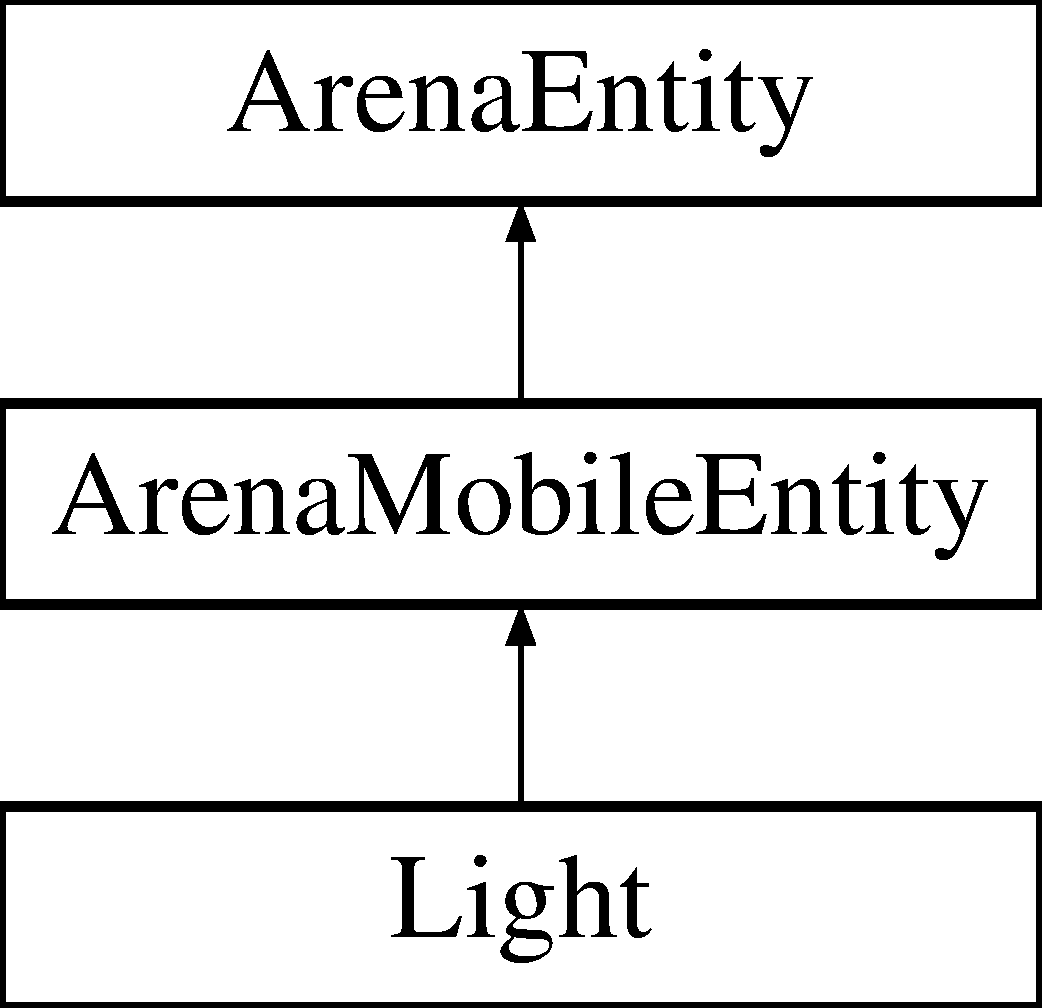
\includegraphics[height=3.000000cm]{class_light}
\end{center}
\end{figure}
\subsection*{Public Member Functions}
\begin{DoxyCompactItemize}
\item 
\mbox{\Hypertarget{class_light_aeb5df09a25a32f19fdffa761268ba24f}\label{class_light_aeb5df09a25a32f19fdffa761268ba24f}} 
\mbox{\hyperlink{class_light_aeb5df09a25a32f19fdffa761268ba24f}{Light}} ()
\begin{DoxyCompactList}\small\item\em Constructor. \end{DoxyCompactList}\item 
\mbox{\Hypertarget{class_light_a49b2e32cf8173353ac4689fdadbb95d5}\label{class_light_a49b2e32cf8173353ac4689fdadbb95d5}} 
std\+::string \mbox{\hyperlink{class_light_a49b2e32cf8173353ac4689fdadbb95d5}{get\+\_\+name}} () const override
\begin{DoxyCompactList}\small\item\em Get the name of the \mbox{\hyperlink{class_light}{Light}} for visualization purposes, and to aid in debugging. \end{DoxyCompactList}\item 
\mbox{\Hypertarget{class_light_a61485eb0684868b503e1b96e6a3206c3}\label{class_light_a61485eb0684868b503e1b96e6a3206c3}} 
void \mbox{\hyperlink{class_light_a61485eb0684868b503e1b96e6a3206c3}{Reset}} () override
\begin{DoxyCompactList}\small\item\em Reset the onstacle to a newly constructed state (needed for reset button to work in G\+UI). \end{DoxyCompactList}\item 
void \mbox{\hyperlink{class_light_a97934eec7489f9b072534f5e30a2d90d}{Timestep\+Update}} (unsigned int dt) override
\begin{DoxyCompactList}\small\item\em Update the \mbox{\hyperlink{class_light}{Light}}\textquotesingle{}s position and velocity after the specified duration has passed. \end{DoxyCompactList}\item 
\mbox{\Hypertarget{class_light_ad8f77c9857b26273d913a18be1311a11}\label{class_light_ad8f77c9857b26273d913a18be1311a11}} 
void \mbox{\hyperlink{class_light_ad8f77c9857b26273d913a18be1311a11}{Handle\+Collision}} (Entity\+Type object\+\_\+type, \mbox{\hyperlink{class_arena_entity}{Arena\+Entity}} $\ast$object=N\+U\+LL) override
\begin{DoxyCompactList}\small\item\em Handles the collision by setting the sensor to activated. \end{DoxyCompactList}\item 
\mbox{\Hypertarget{class_light_a3a8b57cc040b0ab220cbc89d947fd2ab}\label{class_light_a3a8b57cc040b0ab220cbc89d947fd2ab}} 
void \mbox{\hyperlink{class_light_a3a8b57cc040b0ab220cbc89d947fd2ab}{Increase\+Speed}} ()
\begin{DoxyCompactList}\small\item\em Command that comes from the controller, then is passed to handler. \end{DoxyCompactList}\item 
\mbox{\Hypertarget{class_light_ade825fe740b39f80aa934588e29d12f9}\label{class_light_ade825fe740b39f80aa934588e29d12f9}} 
void \mbox{\hyperlink{class_light_ade825fe740b39f80aa934588e29d12f9}{Decrease\+Speed}} ()
\begin{DoxyCompactList}\small\item\em Command that comes from the controller, then is passed to handler. \end{DoxyCompactList}\item 
\mbox{\Hypertarget{class_light_a3d96e80148c96e450007da8358613187}\label{class_light_a3d96e80148c96e450007da8358613187}} 
void \mbox{\hyperlink{class_light_a3d96e80148c96e450007da8358613187}{Turn\+Right}} ()
\begin{DoxyCompactList}\small\item\em Command that comes from the controller, then is passed to handler. \end{DoxyCompactList}\item 
\mbox{\Hypertarget{class_light_a571db6b9e9478fbced0cf9212fa44fb4}\label{class_light_a571db6b9e9478fbced0cf9212fa44fb4}} 
void \mbox{\hyperlink{class_light_a571db6b9e9478fbced0cf9212fa44fb4}{Turn\+Left}} ()
\begin{DoxyCompactList}\small\item\em Command that comes from the controller, then is passed to handler. \end{DoxyCompactList}\item 
\mbox{\Hypertarget{class_light_ac9d27a6f428537303f41831be3ddd526}\label{class_light_ac9d27a6f428537303f41831be3ddd526}} 
\mbox{\hyperlink{class_motion_handler_robot}{Motion\+Handler\+Robot}} {\bfseries get\+\_\+motion\+\_\+handler} ()
\item 
\mbox{\Hypertarget{class_light_af8a67e1e3d3e6b21c169cfd6bdaa8ab2}\label{class_light_af8a67e1e3d3e6b21c169cfd6bdaa8ab2}} 
\mbox{\hyperlink{class_motion_behavior_differential}{Motion\+Behavior\+Differential}} {\bfseries get\+\_\+motion\+\_\+behavior} ()
\end{DoxyCompactItemize}
\subsection*{Additional Inherited Members}


\subsection{Detailed Description}
Class representing an mobile \mbox{\hyperlink{class_light}{Light}} within the \mbox{\hyperlink{class_arena}{Arena}}. 

\subsection{Member Function Documentation}
\mbox{\Hypertarget{class_light_a97934eec7489f9b072534f5e30a2d90d}\label{class_light_a97934eec7489f9b072534f5e30a2d90d}} 
\index{Light@{Light}!Timestep\+Update@{Timestep\+Update}}
\index{Timestep\+Update@{Timestep\+Update}!Light@{Light}}
\subsubsection{\texorpdfstring{Timestep\+Update()}{TimestepUpdate()}}
{\footnotesize\ttfamily void Light\+::\+Timestep\+Update (\begin{DoxyParamCaption}\item[{unsigned int}]{dt }\end{DoxyParamCaption})\hspace{0.3cm}{\ttfamily [override]}}



Update the \mbox{\hyperlink{class_light}{Light}}\textquotesingle{}s position and velocity after the specified duration has passed. 


\begin{DoxyParams}{Parameters}
{\em dt} & The \# of timesteps that have elapsed since the last update. \\
\hline
\end{DoxyParams}


The documentation for this class was generated from the following files\+:\begin{DoxyCompactItemize}
\item 
src/\mbox{\hyperlink{light_8h}{light.\+h}}\item 
src/\mbox{\hyperlink{light_8cc}{light.\+cc}}\end{DoxyCompactItemize}

\hypertarget{class_light_sensor}{}\section{Light\+Sensor Class Reference}
\label{class_light_sensor}\index{Light\+Sensor@{Light\+Sensor}}
Inheritance diagram for Light\+Sensor\+:\begin{figure}[H]
\begin{center}
\leavevmode
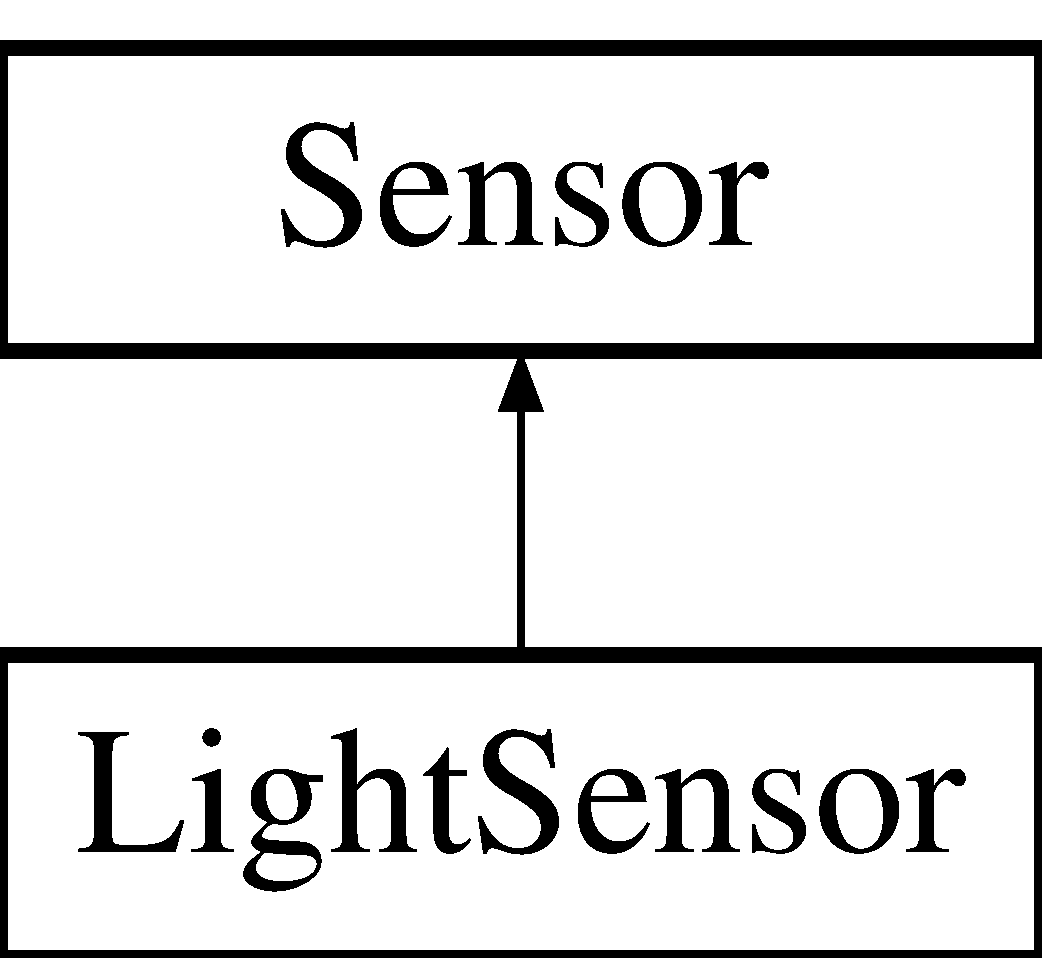
\includegraphics[height=2.000000cm]{class_light_sensor}
\end{center}
\end{figure}
\subsection*{Public Member Functions}
\begin{DoxyCompactItemize}
\item 
\mbox{\Hypertarget{class_light_sensor_ac99ce134fee5ee22775a8d5a6531d02b}\label{class_light_sensor_ac99ce134fee5ee22775a8d5a6531d02b}} 
\mbox{\hyperlink{class_light_sensor_ac99ce134fee5ee22775a8d5a6531d02b}{Light\+Sensor}} (\mbox{\hyperlink{class_arena_mobile_entity}{Arena\+Mobile\+Entity}} $\ast$ent)
\begin{DoxyCompactList}\small\item\em \mbox{\hyperlink{class_arena_entity}{Arena\+Entity}} constructor initialized with default values from \mbox{\hyperlink{params_8h}{params.\+h}}. \end{DoxyCompactList}\item 
\mbox{\Hypertarget{class_light_sensor_abcd9b14b4c09ed48d09eddd72943f898}\label{class_light_sensor_abcd9b14b4c09ed48d09eddd72943f898}} 
int \mbox{\hyperlink{class_light_sensor_abcd9b14b4c09ed48d09eddd72943f898}{Calculate\+Reading}} (\mbox{\hyperlink{class_light}{Light}} $\ast$ent)
\begin{DoxyCompactList}\small\item\em calaculates the reading using the expontial function \end{DoxyCompactList}\item 
\mbox{\Hypertarget{class_light_sensor_a8b8643f10dc619dd8f31ab87034a04f6}\label{class_light_sensor_a8b8643f10dc619dd8f31ab87034a04f6}} 
void \mbox{\hyperlink{class_light_sensor_a8b8643f10dc619dd8f31ab87034a04f6}{Reset}} () override
\begin{DoxyCompactList}\small\item\em resets the sensors reading \end{DoxyCompactList}\item 
\mbox{\Hypertarget{class_light_sensor_ac353ce16128a5bd434fa41cf99b70e3d}\label{class_light_sensor_ac353ce16128a5bd434fa41cf99b70e3d}} 
void \mbox{\hyperlink{class_light_sensor_ac353ce16128a5bd434fa41cf99b70e3d}{update}} (std\+::vector$<$ class \mbox{\hyperlink{class_arena_entity}{Arena\+Entity}} $\ast$$>$ stimili) override
\begin{DoxyCompactList}\small\item\em accumalates the reading by calling the Calculate\+Reading for each light in the arena \end{DoxyCompactList}\end{DoxyCompactItemize}
\subsection*{Additional Inherited Members}


The documentation for this class was generated from the following files\+:\begin{DoxyCompactItemize}
\item 
src/\mbox{\hyperlink{light__sensor_8h}{light\+\_\+sensor.\+h}}\item 
src/\mbox{\hyperlink{light__sensor_8cc}{light\+\_\+sensor.\+cc}}\end{DoxyCompactItemize}

\hypertarget{class_motion_behavior}{}\section{Motion\+Behavior Class Reference}
\label{class_motion_behavior}\index{Motion\+Behavior@{Motion\+Behavior}}


Class managing an \hyperlink{class_arena_mobile_entity}{Arena\+Mobile\+Entity}\textquotesingle{}s position.  




{\ttfamily \#include $<$motion\+\_\+behavior.\+h$>$}

Inheritance diagram for Motion\+Behavior\+:\begin{figure}[H]
\begin{center}
\leavevmode
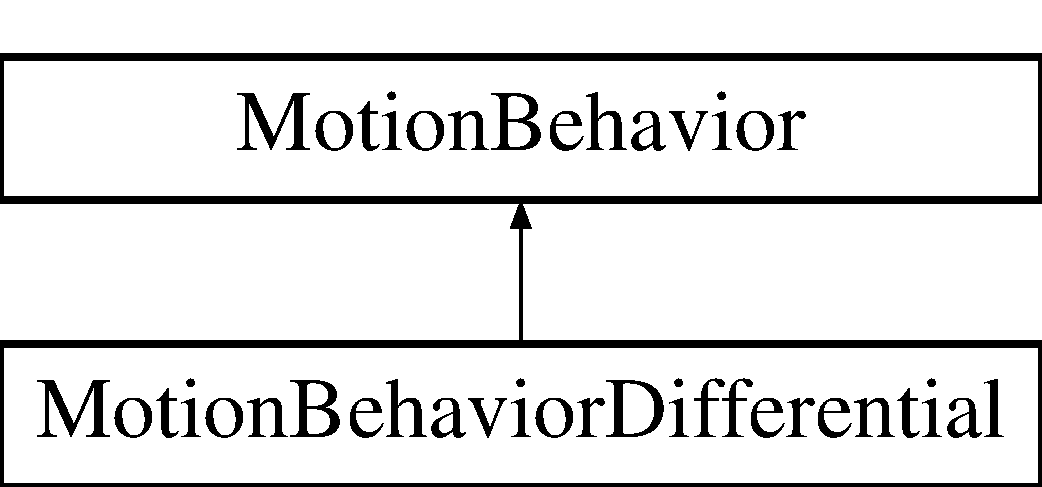
\includegraphics[height=2.000000cm]{class_motion_behavior}
\end{center}
\end{figure}
\subsection*{Public Member Functions}
\begin{DoxyCompactItemize}
\item 
\hyperlink{class_motion_behavior_aa2d5f7d563f4fdb5702edb8367eaa6e7}{Motion\+Behavior} (\hyperlink{class_arena_mobile_entity}{Arena\+Mobile\+Entity} $\ast$ent)\hypertarget{class_motion_behavior_aa2d5f7d563f4fdb5702edb8367eaa6e7}{}\label{class_motion_behavior_aa2d5f7d563f4fdb5702edb8367eaa6e7}

\begin{DoxyCompactList}\small\item\em Default constructor. \end{DoxyCompactList}\item 
{\bfseries Motion\+Behavior} (const \hyperlink{class_motion_behavior}{Motion\+Behavior} \&other)=default\hypertarget{class_motion_behavior_a5fe8e8a49e8cb34519a34ca652a23143}{}\label{class_motion_behavior_a5fe8e8a49e8cb34519a34ca652a23143}

\item 
\hyperlink{class_motion_behavior}{Motion\+Behavior} \& {\bfseries operator=} (const \hyperlink{class_motion_behavior}{Motion\+Behavior} \&other)=default\hypertarget{class_motion_behavior_a227057c1862c64bbc609705205473abc}{}\label{class_motion_behavior_a227057c1862c64bbc609705205473abc}

\item 
virtual void \hyperlink{class_motion_behavior_a804f440bb7f03f19abec79a1ab671494}{Update\+Pose} (double dt, \hyperlink{struct_wheel_velocity}{Wheel\+Velocity} vel=\hyperlink{struct_wheel_velocity}{Wheel\+Velocity}())
\begin{DoxyCompactList}\small\item\em Update the position (and possibly orientation) for an \hyperlink{class_arena_mobile_entity}{Arena\+Mobile\+Entity}, based on its current position and velocity. \end{DoxyCompactList}\item 
\hyperlink{class_arena_mobile_entity}{Arena\+Mobile\+Entity} $\ast$ \hyperlink{class_motion_behavior_a1daf82b16d312ba6f5f71178e7fafa79}{get\+\_\+entity} ()\hypertarget{class_motion_behavior_a1daf82b16d312ba6f5f71178e7fafa79}{}\label{class_motion_behavior_a1daf82b16d312ba6f5f71178e7fafa79}

\begin{DoxyCompactList}\small\item\em Getter of entity in which this class was created. \end{DoxyCompactList}\end{DoxyCompactItemize}
\subsection*{Protected Attributes}
\begin{DoxyCompactItemize}
\item 
\hyperlink{class_arena_mobile_entity}{Arena\+Mobile\+Entity} $\ast$ {\bfseries entity\+\_\+}\hypertarget{class_motion_behavior_a9254cf197657a2a52d89dbc01da31b8f}{}\label{class_motion_behavior_a9254cf197657a2a52d89dbc01da31b8f}

\end{DoxyCompactItemize}


\subsection{Detailed Description}
Class managing an \hyperlink{class_arena_mobile_entity}{Arena\+Mobile\+Entity}\textquotesingle{}s position. 

Update the position based on the current speed and position. This is simple, but the framework allows for more sophisticated models of motion in which each wheel has different speeds. 

\subsection{Member Function Documentation}
\index{Motion\+Behavior@{Motion\+Behavior}!Update\+Pose@{Update\+Pose}}
\index{Update\+Pose@{Update\+Pose}!Motion\+Behavior@{Motion\+Behavior}}
\subsubsection[{\texorpdfstring{Update\+Pose(double dt, Wheel\+Velocity vel=\+Wheel\+Velocity())}{UpdatePose(double dt, WheelVelocity vel=WheelVelocity())}}]{\setlength{\rightskip}{0pt plus 5cm}void Motion\+Behavior\+::\+Update\+Pose (
\begin{DoxyParamCaption}
\item[{double}]{dt, }
\item[{{\bf Wheel\+Velocity}}]{vel = {\ttfamily {\bf Wheel\+Velocity}()}}
\end{DoxyParamCaption}
)\hspace{0.3cm}{\ttfamily [virtual]}}\hypertarget{class_motion_behavior_a804f440bb7f03f19abec79a1ab671494}{}\label{class_motion_behavior_a804f440bb7f03f19abec79a1ab671494}


Update the position (and possibly orientation) for an \hyperlink{class_arena_mobile_entity}{Arena\+Mobile\+Entity}, based on its current position and velocity. 


\begin{DoxyParams}[1]{Parameters}
\mbox{\tt in}  & {\em dt} & \# of timesteps elapsed since the last update. \\
\hline
\mbox{\tt in}  & {\em vel} & \hyperlink{struct_wheel_velocity}{Wheel\+Velocity} stored within the motion handler \\
\hline
\end{DoxyParams}


Reimplemented in \hyperlink{class_motion_behavior_differential_a929c3a05aa2072acf2a508109b1259ef}{Motion\+Behavior\+Differential}.



The documentation for this class was generated from the following files\+:\begin{DoxyCompactItemize}
\item 
src/\hyperlink{motion__behavior_8h}{motion\+\_\+behavior.\+h}\item 
src/\hyperlink{motion__behavior_8cc}{motion\+\_\+behavior.\+cc}\end{DoxyCompactItemize}

\hypertarget{class_motion_behavior_differential}{}\section{Motion\+Behavior\+Differential Class Reference}
\label{class_motion_behavior_differential}\index{Motion\+Behavior\+Differential@{Motion\+Behavior\+Differential}}


A simple model of differential drive kinematics based on the notes here\+: $\sim$https\+://chess.eecs.\+berkeley.\+edu/eecs149/documentation/differential\+Drive.pdf$\sim$.  




{\ttfamily \#include $<$motion\+\_\+behavior\+\_\+differential.\+h$>$}

Inheritance diagram for Motion\+Behavior\+Differential\+:\begin{figure}[H]
\begin{center}
\leavevmode
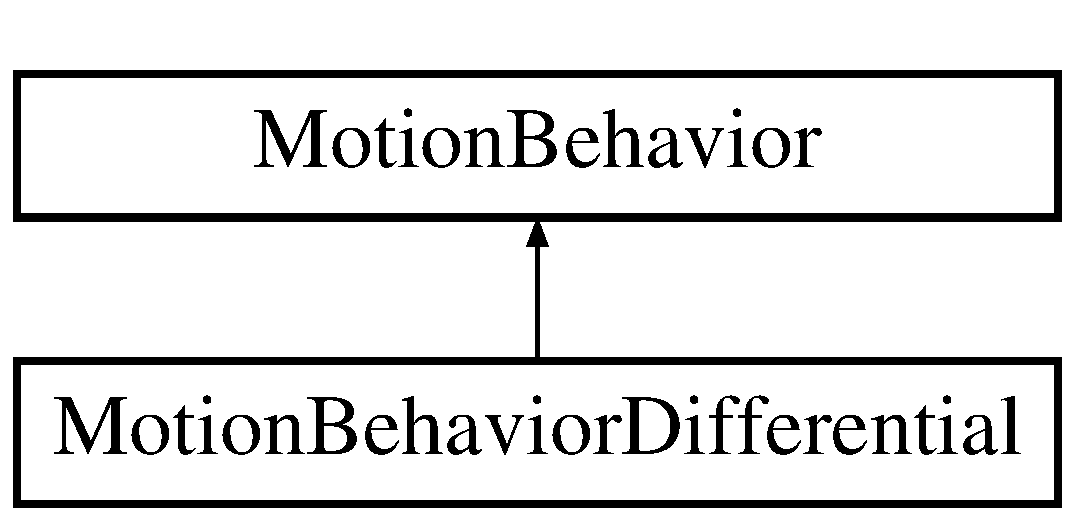
\includegraphics[height=2.000000cm]{class_motion_behavior_differential}
\end{center}
\end{figure}
\subsection*{Public Member Functions}
\begin{DoxyCompactItemize}
\item 
\mbox{\Hypertarget{class_motion_behavior_differential_a8815791ac85212945862454560279d28}\label{class_motion_behavior_differential_a8815791ac85212945862454560279d28}} 
{\bfseries Motion\+Behavior\+Differential} (\mbox{\hyperlink{class_arena_mobile_entity}{Arena\+Mobile\+Entity}} $\ast$entity)
\item 
\mbox{\Hypertarget{class_motion_behavior_differential_aeaa480aac3de205e1d177c4b4ad73ed6}\label{class_motion_behavior_differential_aeaa480aac3de205e1d177c4b4ad73ed6}} 
{\bfseries Motion\+Behavior\+Differential} (const \mbox{\hyperlink{class_motion_behavior_differential}{Motion\+Behavior\+Differential}} \&other)=default
\item 
\mbox{\Hypertarget{class_motion_behavior_differential_aaf4edbc2e349cb8cdbb033b16b1aef22}\label{class_motion_behavior_differential_aaf4edbc2e349cb8cdbb033b16b1aef22}} 
\mbox{\hyperlink{class_motion_behavior_differential}{Motion\+Behavior\+Differential}} \& {\bfseries operator=} (const \mbox{\hyperlink{class_motion_behavior_differential}{Motion\+Behavior\+Differential}} \&other)=default
\item 
void \mbox{\hyperlink{class_motion_behavior_differential_a929c3a05aa2072acf2a508109b1259ef}{Update\+Pose}} (double dt, \mbox{\hyperlink{struct_wheel_velocity}{Wheel\+Velocity}} vel) override
\begin{DoxyCompactList}\small\item\em Update the pose of an entity based on its current position and how many seconds have elapsed since the last update. \end{DoxyCompactList}\end{DoxyCompactItemize}
\subsection*{Additional Inherited Members}


\subsection{Detailed Description}
A simple model of differential drive kinematics based on the notes here\+: $\sim$https\+://chess.eecs.\+berkeley.\+edu/eecs149/documentation/differential\+Drive.pdf$\sim$. 

\subsection{Member Function Documentation}
\mbox{\Hypertarget{class_motion_behavior_differential_a929c3a05aa2072acf2a508109b1259ef}\label{class_motion_behavior_differential_a929c3a05aa2072acf2a508109b1259ef}} 
\index{Motion\+Behavior\+Differential@{Motion\+Behavior\+Differential}!Update\+Pose@{Update\+Pose}}
\index{Update\+Pose@{Update\+Pose}!Motion\+Behavior\+Differential@{Motion\+Behavior\+Differential}}
\subsubsection{\texorpdfstring{Update\+Pose()}{UpdatePose()}}
{\footnotesize\ttfamily void Motion\+Behavior\+Differential\+::\+Update\+Pose (\begin{DoxyParamCaption}\item[{double}]{dt,  }\item[{\mbox{\hyperlink{struct_wheel_velocity}{Wheel\+Velocity}}}]{vel }\end{DoxyParamCaption})\hspace{0.3cm}{\ttfamily [override]}, {\ttfamily [virtual]}}



Update the pose of an entity based on its current position and how many seconds have elapsed since the last update. 


\begin{DoxyParams}[1]{Parameters}
\mbox{\tt in}  & {\em dt} & Elapsed time interval. \\
\hline
\mbox{\tt in}  & {\em vel} & The \mbox{\hyperlink{struct_wheel_velocity}{Wheel\+Velocity}} stored within the motion handler.\\
\hline
\end{DoxyParams}
Calculates the new pose (i.\+e. position and heading) based on a model of differential drive. If both wheels have equivalent velocity, it travels in the direction of its heading. If one wheel is faster than the other, this drives the entity in an arc (e.\+g. if Wheel\+Velocity.\+right $>$ .left, then the entity will move in an arc turning to the left relative to its heading.) 

Reimplemented from \mbox{\hyperlink{class_motion_behavior_a804f440bb7f03f19abec79a1ab671494}{Motion\+Behavior}}.



The documentation for this class was generated from the following files\+:\begin{DoxyCompactItemize}
\item 
src/\mbox{\hyperlink{motion__behavior__differential_8h}{motion\+\_\+behavior\+\_\+differential.\+h}}\item 
src/motion\+\_\+behavior\+\_\+differential.\+cc\end{DoxyCompactItemize}

\hypertarget{class_motion_handler}{}\section{Motion\+Handler Class Reference}
\label{class_motion_handler}\index{Motion\+Handler@{Motion\+Handler}}


Base class for managing the pose and wheel velocity of the entity.  




{\ttfamily \#include $<$motion\+\_\+handler.\+h$>$}

Inheritance diagram for Motion\+Handler\+:\begin{figure}[H]
\begin{center}
\leavevmode
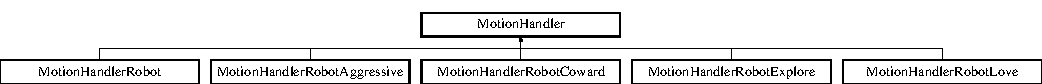
\includegraphics[height=1.125628cm]{class_motion_handler}
\end{center}
\end{figure}
\subsection*{Public Member Functions}
\begin{DoxyCompactItemize}
\item 
\mbox{\Hypertarget{class_motion_handler_a48c0070bfda6acb8a7493eb7fe1200c4}\label{class_motion_handler_a48c0070bfda6acb8a7493eb7fe1200c4}} 
\mbox{\hyperlink{class_motion_handler_a48c0070bfda6acb8a7493eb7fe1200c4}{Motion\+Handler}} (\mbox{\hyperlink{class_arena_mobile_entity}{Arena\+Mobile\+Entity}} $\ast$ent)
\begin{DoxyCompactList}\small\item\em Constructor. \end{DoxyCompactList}\item 
\mbox{\Hypertarget{class_motion_handler_a91dc98beab9d5ccce6b6c18ce32c0488}\label{class_motion_handler_a91dc98beab9d5ccce6b6c18ce32c0488}} 
{\bfseries Motion\+Handler} (const \mbox{\hyperlink{class_motion_handler}{Motion\+Handler}} \&other)=default
\item 
\mbox{\Hypertarget{class_motion_handler_ad45188f2d9794fd2b257d586a7b522e6}\label{class_motion_handler_ad45188f2d9794fd2b257d586a7b522e6}} 
\mbox{\hyperlink{class_motion_handler}{Motion\+Handler}} \& {\bfseries operator=} (const \mbox{\hyperlink{class_motion_handler}{Motion\+Handler}} \&other)=default
\item 
\mbox{\Hypertarget{class_motion_handler_ad9bfac3d0ec3cec1d607f41475886c3c}\label{class_motion_handler_ad9bfac3d0ec3cec1d607f41475886c3c}} 
virtual void \mbox{\hyperlink{class_motion_handler_ad9bfac3d0ec3cec1d607f41475886c3c}{Update\+Velocity}} ()
\begin{DoxyCompactList}\small\item\em Update the heading angle according to the touch sensor reading. \end{DoxyCompactList}\item 
\mbox{\Hypertarget{class_motion_handler_ada53f0d6e25d759fc3f45cc55d440177}\label{class_motion_handler_ada53f0d6e25d759fc3f45cc55d440177}} 
double \mbox{\hyperlink{class_motion_handler_ada53f0d6e25d759fc3f45cc55d440177}{get\+\_\+speed\+\_\+delta}} () const
\begin{DoxyCompactList}\small\item\em Getter for speed delta used when user requests speed increase. \end{DoxyCompactList}\item 
\mbox{\Hypertarget{class_motion_handler_a908b330346b3fe969684106bd5c7619d}\label{class_motion_handler_a908b330346b3fe969684106bd5c7619d}} 
void \mbox{\hyperlink{class_motion_handler_a908b330346b3fe969684106bd5c7619d}{set\+\_\+speed\+\_\+delta}} (double sd)
\begin{DoxyCompactList}\small\item\em Setter method for the speed delta. Set at initialization only. \end{DoxyCompactList}\item 
\mbox{\Hypertarget{class_motion_handler_aa5ec33068c516234a6521de356b08d68}\label{class_motion_handler_aa5ec33068c516234a6521de356b08d68}} 
double \mbox{\hyperlink{class_motion_handler_aa5ec33068c516234a6521de356b08d68}{get\+\_\+angle\+\_\+delta}} () const
\begin{DoxyCompactList}\small\item\em Getter for angle delta used when user requests turning. \end{DoxyCompactList}\item 
\mbox{\Hypertarget{class_motion_handler_a8c2811ddf1a0f077fec829c460009286}\label{class_motion_handler_a8c2811ddf1a0f077fec829c460009286}} 
void \mbox{\hyperlink{class_motion_handler_a8c2811ddf1a0f077fec829c460009286}{set\+\_\+angle\+\_\+delta}} (double ad)
\begin{DoxyCompactList}\small\item\em Setter method for the angle delta. Set at initialization only. \end{DoxyCompactList}\item 
\mbox{\Hypertarget{class_motion_handler_af6b91f5626075b09dba3d14177213622}\label{class_motion_handler_af6b91f5626075b09dba3d14177213622}} 
virtual void \mbox{\hyperlink{class_motion_handler_af6b91f5626075b09dba3d14177213622}{Increase\+Speed}} ()
\begin{DoxyCompactList}\small\item\em Increase the overall speed of the entity by speed\+\_\+delta. \end{DoxyCompactList}\item 
\mbox{\Hypertarget{class_motion_handler_a25ad77fb1a4c79f8303a256b7e1cbc9c}\label{class_motion_handler_a25ad77fb1a4c79f8303a256b7e1cbc9c}} 
virtual void \mbox{\hyperlink{class_motion_handler_a25ad77fb1a4c79f8303a256b7e1cbc9c}{Decrease\+Speed}} ()
\begin{DoxyCompactList}\small\item\em Decrease the overall speed of the entity by speed\+\_\+delta. \end{DoxyCompactList}\item 
\mbox{\Hypertarget{class_motion_handler_a22b99a21307a534165d811740d8aeac1}\label{class_motion_handler_a22b99a21307a534165d811740d8aeac1}} 
virtual void \mbox{\hyperlink{class_motion_handler_a22b99a21307a534165d811740d8aeac1}{Turn\+Right}} ()
\begin{DoxyCompactList}\small\item\em Turn the entity to the right by angle\+\_\+delta (in degrees?) \end{DoxyCompactList}\item 
\mbox{\Hypertarget{class_motion_handler_a922e3dd8c6a98b54607837c5e669c557}\label{class_motion_handler_a922e3dd8c6a98b54607837c5e669c557}} 
virtual void \mbox{\hyperlink{class_motion_handler_a922e3dd8c6a98b54607837c5e669c557}{Turn\+Left}} ()
\begin{DoxyCompactList}\small\item\em Turn the entity to the left by angle\+\_\+delta (in degrees?) \end{DoxyCompactList}\item 
\mbox{\Hypertarget{class_motion_handler_aa04a0d87165965ea7ba8be6b21cfa0cf}\label{class_motion_handler_aa04a0d87165965ea7ba8be6b21cfa0cf}} 
virtual void \mbox{\hyperlink{class_motion_handler_aa04a0d87165965ea7ba8be6b21cfa0cf}{Stop}} ()
\begin{DoxyCompactList}\small\item\em stop the entity to be at zero velocity. \end{DoxyCompactList}\item 
\mbox{\Hypertarget{class_motion_handler_a71e2e4cdddfb8c49eb18cf41878a08c0}\label{class_motion_handler_a71e2e4cdddfb8c49eb18cf41878a08c0}} 
double \mbox{\hyperlink{class_motion_handler_a71e2e4cdddfb8c49eb18cf41878a08c0}{get\+\_\+max\+\_\+speed}} () const
\begin{DoxyCompactList}\small\item\em Getter method for the maximum speed of entity. \end{DoxyCompactList}\item 
\mbox{\Hypertarget{class_motion_handler_a32e832d35e73e9db85c16b3ff569196e}\label{class_motion_handler_a32e832d35e73e9db85c16b3ff569196e}} 
void \mbox{\hyperlink{class_motion_handler_a32e832d35e73e9db85c16b3ff569196e}{set\+\_\+max\+\_\+speed}} (double ms)
\begin{DoxyCompactList}\small\item\em Setter method for the maximum speed. Set at initialization only. \end{DoxyCompactList}\item 
\mbox{\Hypertarget{class_motion_handler_af6ef42cdbf31ec1589e14d5dfd639d79}\label{class_motion_handler_af6ef42cdbf31ec1589e14d5dfd639d79}} 
double \mbox{\hyperlink{class_motion_handler_af6ef42cdbf31ec1589e14d5dfd639d79}{get\+\_\+max\+\_\+angle}} () const
\begin{DoxyCompactList}\small\item\em Getter method for the maximum angle. \end{DoxyCompactList}\item 
\mbox{\Hypertarget{class_motion_handler_aa73973c705626f1f95ac59391f23bcc9}\label{class_motion_handler_aa73973c705626f1f95ac59391f23bcc9}} 
void \mbox{\hyperlink{class_motion_handler_aa73973c705626f1f95ac59391f23bcc9}{set\+\_\+max\+\_\+angle}} (double ma)
\begin{DoxyCompactList}\small\item\em Setter method for the maximum angle. Set at initialization only. \end{DoxyCompactList}\item 
\mbox{\Hypertarget{class_motion_handler_abe03a52474984233d1867405925a4102}\label{class_motion_handler_abe03a52474984233d1867405925a4102}} 
\mbox{\hyperlink{struct_wheel_velocity}{Wheel\+Velocity}} \mbox{\hyperlink{class_motion_handler_abe03a52474984233d1867405925a4102}{get\+\_\+velocity}} () const
\begin{DoxyCompactList}\small\item\em Getter for \mbox{\hyperlink{struct_wheel_velocity}{Wheel\+Velocity}} struct, which has a .left and .right value. \end{DoxyCompactList}\item 
\mbox{\Hypertarget{class_motion_handler_ac4bf67ba783c1afb5a5839229de3f3f9}\label{class_motion_handler_ac4bf67ba783c1afb5a5839229de3f3f9}} 
void \mbox{\hyperlink{class_motion_handler_ac4bf67ba783c1afb5a5839229de3f3f9}{set\+\_\+velocity}} (\mbox{\hyperlink{struct_wheel_velocity}{Wheel\+Velocity}} vel)
\begin{DoxyCompactList}\small\item\em Setter for \mbox{\hyperlink{struct_wheel_velocity}{Wheel\+Velocity}} struct with struct as input param. \end{DoxyCompactList}\item 
\mbox{\Hypertarget{class_motion_handler_af31975aa667ca20835e4d5bb0216706e}\label{class_motion_handler_af31975aa667ca20835e4d5bb0216706e}} 
void \mbox{\hyperlink{class_motion_handler_af31975aa667ca20835e4d5bb0216706e}{set\+\_\+velocity}} (double vl, double vr)
\begin{DoxyCompactList}\small\item\em Setter for \mbox{\hyperlink{struct_wheel_velocity}{Wheel\+Velocity}} struct with input params of .left and .right components. \end{DoxyCompactList}\item 
\mbox{\Hypertarget{class_motion_handler_ad8472612d15be1ada7f919f45d245adc}\label{class_motion_handler_ad8472612d15be1ada7f919f45d245adc}} 
\mbox{\hyperlink{class_arena_mobile_entity}{Arena\+Mobile\+Entity}} $\ast$ {\bfseries get\+\_\+entity} ()
\item 
\mbox{\Hypertarget{class_motion_handler_a96451327dddb6a7d7eef689498abbde2}\label{class_motion_handler_a96451327dddb6a7d7eef689498abbde2}} 
void {\bfseries set\+\_\+lightsensor\+\_\+reading} (double left\+\_\+reading, double right\+\_\+reading)
\item 
\mbox{\Hypertarget{class_motion_handler_ab7959aa3946b9a91570a990e0350f538}\label{class_motion_handler_ab7959aa3946b9a91570a990e0350f538}} 
double {\bfseries get\+\_\+left\+\_\+sensor\+\_\+reading} ()
\item 
\mbox{\Hypertarget{class_motion_handler_ac97d180150dade9601bbed25a248f150}\label{class_motion_handler_ac97d180150dade9601bbed25a248f150}} 
double {\bfseries get\+\_\+right\+\_\+sensor\+\_\+reading} ()
\item 
\mbox{\Hypertarget{class_motion_handler_a2fadcc5b46f73af637732ffc35e0a9a9}\label{class_motion_handler_a2fadcc5b46f73af637732ffc35e0a9a9}} 
double {\bfseries get\+\_\+right\+\_\+food\+\_\+sensor\+\_\+reading} ()
\item 
\mbox{\Hypertarget{class_motion_handler_a23c4bc0d6ce0657c7007c59380bf2d48}\label{class_motion_handler_a23c4bc0d6ce0657c7007c59380bf2d48}} 
double {\bfseries get\+\_\+left\+\_\+food\+\_\+sensor\+\_\+reading} ()
\item 
\mbox{\Hypertarget{class_motion_handler_ad3d6d67491b4b06fc85902a12cc21699}\label{class_motion_handler_ad3d6d67491b4b06fc85902a12cc21699}} 
void {\bfseries set\+\_\+foodsensor\+\_\+reading} (double left\+\_\+food\+\_\+reading, double right\+\_\+food\+\_\+reading)
\end{DoxyCompactItemize}
\subsection*{Protected Attributes}
\begin{DoxyCompactItemize}
\item 
\mbox{\Hypertarget{class_motion_handler_a659fd1ec8878260a63779bf45681f5a4}\label{class_motion_handler_a659fd1ec8878260a63779bf45681f5a4}} 
\mbox{\hyperlink{class_arena_mobile_entity}{Arena\+Mobile\+Entity}} $\ast$ {\bfseries entity\+\_\+}
\end{DoxyCompactItemize}


\subsection{Detailed Description}
Base class for managing the pose and wheel velocity of the entity. 

The pose.\+heading will change when the entity collides. The pose position will change at each timestep, which is determined by the motion behavior, not the handler. The pose.\+heading might change at each timestep (if wheel velocities are not equivalent), again determined by the motion behavior. 

The documentation for this class was generated from the following file\+:\begin{DoxyCompactItemize}
\item 
src/\mbox{\hyperlink{motion__handler_8h}{motion\+\_\+handler.\+h}}\end{DoxyCompactItemize}

\hypertarget{class_motion_handler_robot}{}\section{Motion\+Handler\+Robot Class Reference}
\label{class_motion_handler_robot}\index{Motion\+Handler\+Robot@{Motion\+Handler\+Robot}}


Class managing a \mbox{\hyperlink{class_robot}{Robot}}\textquotesingle{}s and \mbox{\hyperlink{class_light}{Light}}\textquotesingle{}s speed and heading angle based on collisions and user inputs.  




{\ttfamily \#include $<$motion\+\_\+handler\+\_\+robot.\+h$>$}

Inheritance diagram for Motion\+Handler\+Robot\+:\begin{figure}[H]
\begin{center}
\leavevmode
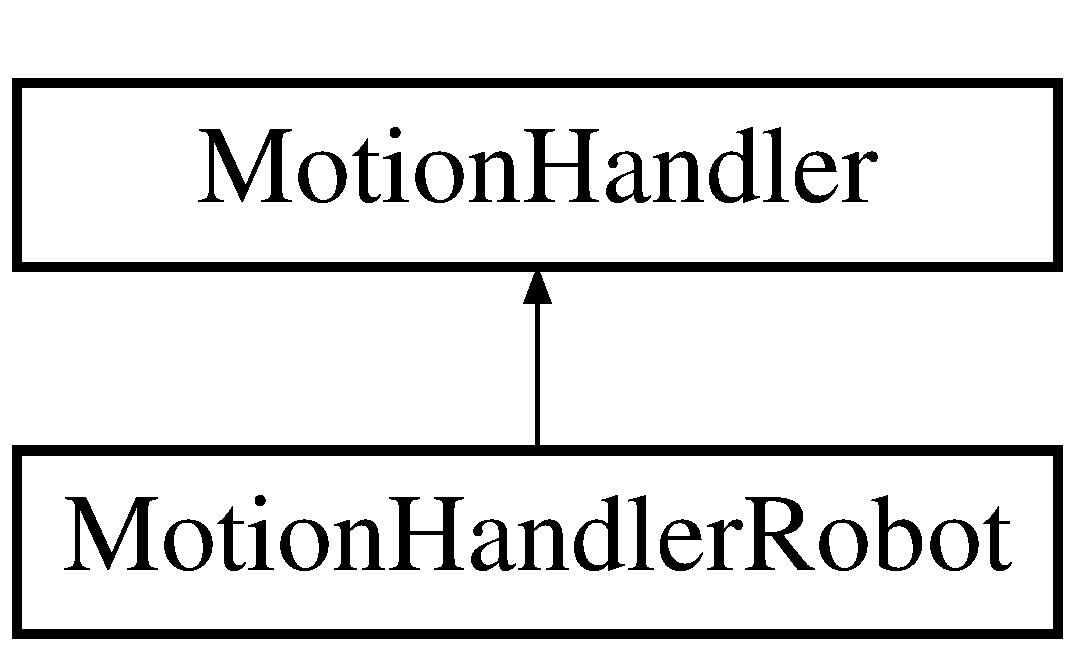
\includegraphics[height=2.000000cm]{class_motion_handler_robot}
\end{center}
\end{figure}
\subsection*{Public Member Functions}
\begin{DoxyCompactItemize}
\item 
\mbox{\Hypertarget{class_motion_handler_robot_a4b52a0b181837a8d63c39f71811d691b}\label{class_motion_handler_robot_a4b52a0b181837a8d63c39f71811d691b}} 
{\bfseries Motion\+Handler\+Robot} (\mbox{\hyperlink{class_arena_mobile_entity}{Arena\+Mobile\+Entity}} $\ast$ent)
\item 
\mbox{\Hypertarget{class_motion_handler_robot_a66445cc9057e3ef9298b5bd239df6d4e}\label{class_motion_handler_robot_a66445cc9057e3ef9298b5bd239df6d4e}} 
{\bfseries Motion\+Handler\+Robot} (const \mbox{\hyperlink{class_motion_handler_robot}{Motion\+Handler\+Robot}} \&other)=default
\item 
\mbox{\Hypertarget{class_motion_handler_robot_a48181f197ffb864f16e29721ad964e4a}\label{class_motion_handler_robot_a48181f197ffb864f16e29721ad964e4a}} 
\mbox{\hyperlink{class_motion_handler_robot}{Motion\+Handler\+Robot}} \& {\bfseries operator=} (const \mbox{\hyperlink{class_motion_handler_robot}{Motion\+Handler\+Robot}} \&other)=default
\item 
\mbox{\Hypertarget{class_motion_handler_robot_acd2cdb615d806dcf809142e84569ca9d}\label{class_motion_handler_robot_acd2cdb615d806dcf809142e84569ca9d}} 
void \mbox{\hyperlink{class_motion_handler_robot_acd2cdb615d806dcf809142e84569ca9d}{Update\+Velocity}} () override
\begin{DoxyCompactList}\small\item\em Update the speed and the pose angle according to the sensor readings. \end{DoxyCompactList}\item 
\mbox{\Hypertarget{class_motion_handler_robot_a93ea16501b7b8c0bd78edb2681aa3b6d}\label{class_motion_handler_robot_a93ea16501b7b8c0bd78edb2681aa3b6d}} 
void \mbox{\hyperlink{class_motion_handler_robot_a93ea16501b7b8c0bd78edb2681aa3b6d}{Increase\+Speed}} () override
\begin{DoxyCompactList}\small\item\em Increase the overall speed of the entity by speed\+\_\+delta. \end{DoxyCompactList}\item 
\mbox{\Hypertarget{class_motion_handler_robot_a89e9b8b4e22fb021d7d67c817e66b7b2}\label{class_motion_handler_robot_a89e9b8b4e22fb021d7d67c817e66b7b2}} 
void \mbox{\hyperlink{class_motion_handler_robot_a89e9b8b4e22fb021d7d67c817e66b7b2}{Decrease\+Speed}} () override
\begin{DoxyCompactList}\small\item\em Decrease the overall speed of the entity by speed\+\_\+delta. \end{DoxyCompactList}\item 
\mbox{\Hypertarget{class_motion_handler_robot_a4b18204b7c7f7f8a3cbb7f0e8ccf088f}\label{class_motion_handler_robot_a4b18204b7c7f7f8a3cbb7f0e8ccf088f}} 
void \mbox{\hyperlink{class_motion_handler_robot_a4b18204b7c7f7f8a3cbb7f0e8ccf088f}{Turn\+Right}} () override
\begin{DoxyCompactList}\small\item\em Turn the entity to the right by angle\+\_\+delta (in degrees?) \end{DoxyCompactList}\item 
\mbox{\Hypertarget{class_motion_handler_robot_a955ca2693c4188ffb08cfde469e58252}\label{class_motion_handler_robot_a955ca2693c4188ffb08cfde469e58252}} 
void \mbox{\hyperlink{class_motion_handler_robot_a955ca2693c4188ffb08cfde469e58252}{Turn\+Left}} () override
\begin{DoxyCompactList}\small\item\em Turn the entity to the left by angle\+\_\+delta (in degrees?) \end{DoxyCompactList}\item 
\mbox{\Hypertarget{class_motion_handler_robot_a735287a2ab240ae0655def3afb0839f1}\label{class_motion_handler_robot_a735287a2ab240ae0655def3afb0839f1}} 
void \mbox{\hyperlink{class_motion_handler_robot_a735287a2ab240ae0655def3afb0839f1}{Stop}} () override
\begin{DoxyCompactList}\small\item\em stop the entity to be at zero velocity. \end{DoxyCompactList}\end{DoxyCompactItemize}
\subsection*{Additional Inherited Members}


\subsection{Detailed Description}
Class managing a \mbox{\hyperlink{class_robot}{Robot}}\textquotesingle{}s and \mbox{\hyperlink{class_light}{Light}}\textquotesingle{}s speed and heading angle based on collisions and user inputs. 

The documentation for this class was generated from the following files\+:\begin{DoxyCompactItemize}
\item 
src/\mbox{\hyperlink{motion__handler__robot_8h}{motion\+\_\+handler\+\_\+robot.\+h}}\item 
src/\mbox{\hyperlink{motion__handler__robot_8cc}{motion\+\_\+handler\+\_\+robot.\+cc}}\end{DoxyCompactItemize}

\hypertarget{class_motion_handler_robot_aggressive}{}\section{Motion\+Handler\+Robot\+Aggressive Class Reference}
\label{class_motion_handler_robot_aggressive}\index{Motion\+Handler\+Robot\+Aggressive@{Motion\+Handler\+Robot\+Aggressive}}


Class managing a \hyperlink{class_robot}{Robot}\textquotesingle{}s and \hyperlink{class_light}{Light}\textquotesingle{}s speed and heading angle based on aggressive sensor readings.  




{\ttfamily \#include $<$motion\+\_\+handler\+\_\+robot\+\_\+aggressive.\+h$>$}

Inheritance diagram for Motion\+Handler\+Robot\+Aggressive\+:\begin{figure}[H]
\begin{center}
\leavevmode
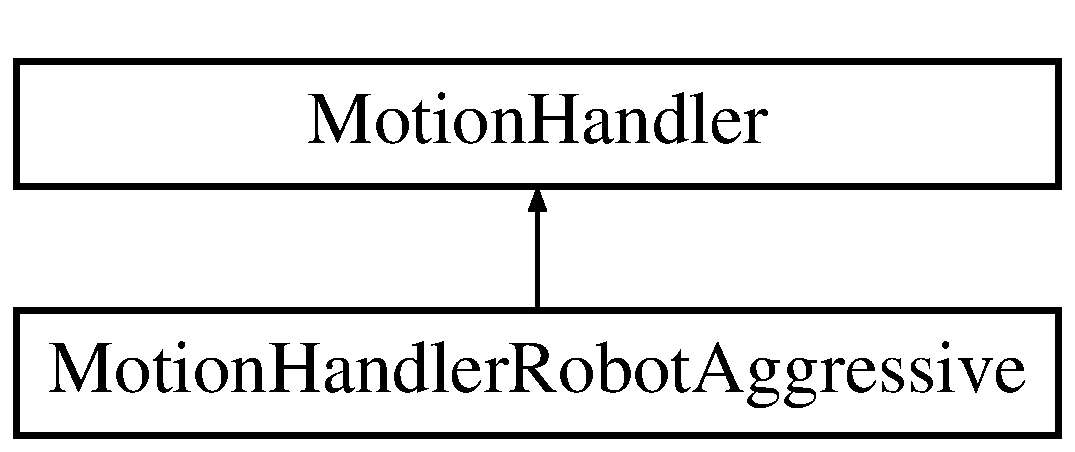
\includegraphics[height=2.000000cm]{class_motion_handler_robot_aggressive}
\end{center}
\end{figure}
\subsection*{Public Member Functions}
\begin{DoxyCompactItemize}
\item 
{\bfseries Motion\+Handler\+Robot\+Aggressive} (\hyperlink{class_arena_mobile_entity}{Arena\+Mobile\+Entity} $\ast$ent)\hypertarget{class_motion_handler_robot_aggressive_acf648d0f2f208acae95758437a426299}{}\label{class_motion_handler_robot_aggressive_acf648d0f2f208acae95758437a426299}

\item 
{\bfseries Motion\+Handler\+Robot\+Aggressive} (const \hyperlink{class_motion_handler_robot_aggressive}{Motion\+Handler\+Robot\+Aggressive} \&other)=default\hypertarget{class_motion_handler_robot_aggressive_a044bb32eea5f808939acd90964b4e1c4}{}\label{class_motion_handler_robot_aggressive_a044bb32eea5f808939acd90964b4e1c4}

\item 
\hyperlink{class_motion_handler_robot_aggressive}{Motion\+Handler\+Robot\+Aggressive} \& {\bfseries operator=} (const \hyperlink{class_motion_handler_robot_aggressive}{Motion\+Handler\+Robot\+Aggressive} \&o)=default\hypertarget{class_motion_handler_robot_aggressive_a7fc4c7bc46c31da2cd51b3cbce16d1d9}{}\label{class_motion_handler_robot_aggressive_a7fc4c7bc46c31da2cd51b3cbce16d1d9}

\item 
void \hyperlink{class_motion_handler_robot_aggressive_ac8bee64034c5fbf46dfce6de36b61dbe}{Update\+Velocity} () override\hypertarget{class_motion_handler_robot_aggressive_ac8bee64034c5fbf46dfce6de36b61dbe}{}\label{class_motion_handler_robot_aggressive_ac8bee64034c5fbf46dfce6de36b61dbe}

\begin{DoxyCompactList}\small\item\em Update the speed and the pose angle according to the aggressive sensor readings. \end{DoxyCompactList}\item 
void \hyperlink{class_motion_handler_robot_aggressive_afb955c958c2b1670e023cf7b6587cce6}{Increase\+Speed} () override\hypertarget{class_motion_handler_robot_aggressive_afb955c958c2b1670e023cf7b6587cce6}{}\label{class_motion_handler_robot_aggressive_afb955c958c2b1670e023cf7b6587cce6}

\begin{DoxyCompactList}\small\item\em Increase the overall speed of the entity by speed\+\_\+delta. \end{DoxyCompactList}\item 
void \hyperlink{class_motion_handler_robot_aggressive_a3f356f4caa6bdbed06c951f27a5cad76}{Decrease\+Speed} () override\hypertarget{class_motion_handler_robot_aggressive_a3f356f4caa6bdbed06c951f27a5cad76}{}\label{class_motion_handler_robot_aggressive_a3f356f4caa6bdbed06c951f27a5cad76}

\begin{DoxyCompactList}\small\item\em Decrease the overall speed of the entity by speed\+\_\+delta. \end{DoxyCompactList}\item 
void \hyperlink{class_motion_handler_robot_aggressive_a848029187d0e50d64a2a1b91a0f7c541}{Turn\+Right} () override\hypertarget{class_motion_handler_robot_aggressive_a848029187d0e50d64a2a1b91a0f7c541}{}\label{class_motion_handler_robot_aggressive_a848029187d0e50d64a2a1b91a0f7c541}

\begin{DoxyCompactList}\small\item\em Turn the entity to the right by angle\+\_\+delta (in degrees?) \end{DoxyCompactList}\item 
void \hyperlink{class_motion_handler_robot_aggressive_a67f0e31a85f979273896433ddfb38a61}{Turn\+Left} () override\hypertarget{class_motion_handler_robot_aggressive_a67f0e31a85f979273896433ddfb38a61}{}\label{class_motion_handler_robot_aggressive_a67f0e31a85f979273896433ddfb38a61}

\begin{DoxyCompactList}\small\item\em Turn the entity to the left by angle\+\_\+delta (in degrees?) \end{DoxyCompactList}\item 
void \hyperlink{class_motion_handler_robot_aggressive_a8c4e7489817fb53fda12a17bc044d76b}{Stop} () override\hypertarget{class_motion_handler_robot_aggressive_a8c4e7489817fb53fda12a17bc044d76b}{}\label{class_motion_handler_robot_aggressive_a8c4e7489817fb53fda12a17bc044d76b}

\begin{DoxyCompactList}\small\item\em stop the entity to be at zero velocity. \end{DoxyCompactList}\end{DoxyCompactItemize}
\subsection*{Additional Inherited Members}


\subsection{Detailed Description}
Class managing a \hyperlink{class_robot}{Robot}\textquotesingle{}s and \hyperlink{class_light}{Light}\textquotesingle{}s speed and heading angle based on aggressive sensor readings. 

The documentation for this class was generated from the following files\+:\begin{DoxyCompactItemize}
\item 
src/\hyperlink{motion__handler__robot__aggressive_8h}{motion\+\_\+handler\+\_\+robot\+\_\+aggressive.\+h}\item 
src/\hyperlink{motion__handler__robot__aggressive_8cc}{motion\+\_\+handler\+\_\+robot\+\_\+aggressive.\+cc}\end{DoxyCompactItemize}

\hypertarget{class_motion_handler_robot_coward}{}\section{Motion\+Handler\+Robot\+Coward Class Reference}
\label{class_motion_handler_robot_coward}\index{Motion\+Handler\+Robot\+Coward@{Motion\+Handler\+Robot\+Coward}}


Class managing a \hyperlink{class_robot}{Robot}\textquotesingle{}s and \hyperlink{class_light}{Light}\textquotesingle{}s speed and heading angle based on coward sesnor reading.  




{\ttfamily \#include $<$motion\+\_\+handler\+\_\+robot\+\_\+coward.\+h$>$}

Inheritance diagram for Motion\+Handler\+Robot\+Coward\+:\begin{figure}[H]
\begin{center}
\leavevmode
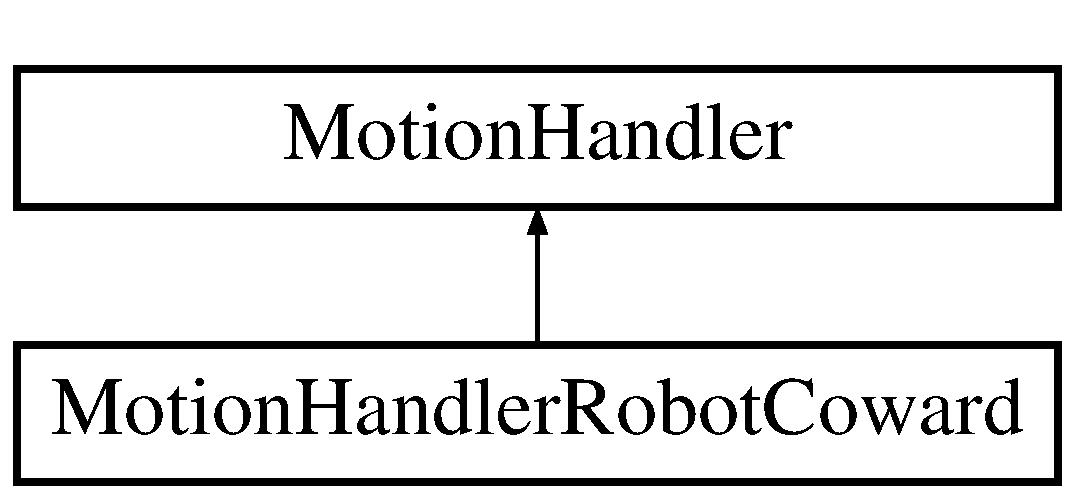
\includegraphics[height=2.000000cm]{class_motion_handler_robot_coward}
\end{center}
\end{figure}
\subsection*{Public Member Functions}
\begin{DoxyCompactItemize}
\item 
{\bfseries Motion\+Handler\+Robot\+Coward} (\hyperlink{class_arena_mobile_entity}{Arena\+Mobile\+Entity} $\ast$ent)\hypertarget{class_motion_handler_robot_coward_a51242788c5a3ca3dc46530a14ab8e301}{}\label{class_motion_handler_robot_coward_a51242788c5a3ca3dc46530a14ab8e301}

\item 
{\bfseries Motion\+Handler\+Robot\+Coward} (const \hyperlink{class_motion_handler_robot_coward}{Motion\+Handler\+Robot\+Coward} \&other)=default\hypertarget{class_motion_handler_robot_coward_ae650416cd316871701127a288eed709a}{}\label{class_motion_handler_robot_coward_ae650416cd316871701127a288eed709a}

\item 
\hyperlink{class_motion_handler_robot_coward}{Motion\+Handler\+Robot\+Coward} \& {\bfseries operator=} (const \hyperlink{class_motion_handler_robot_coward}{Motion\+Handler\+Robot\+Coward} \&other)=default\hypertarget{class_motion_handler_robot_coward_a3bcc3dd802154daf29fa2740bd6c31ae}{}\label{class_motion_handler_robot_coward_a3bcc3dd802154daf29fa2740bd6c31ae}

\item 
void \hyperlink{class_motion_handler_robot_coward_a5f4f03d6128a7d19b2c36af433a17cfd}{Update\+Velocity} () override\hypertarget{class_motion_handler_robot_coward_a5f4f03d6128a7d19b2c36af433a17cfd}{}\label{class_motion_handler_robot_coward_a5f4f03d6128a7d19b2c36af433a17cfd}

\begin{DoxyCompactList}\small\item\em Update the speed and the pose angle according to the sensor readings. \end{DoxyCompactList}\item 
void \hyperlink{class_motion_handler_robot_coward_a22416ce3267987817dc3aba02bfb5d7b}{Increase\+Speed} () override\hypertarget{class_motion_handler_robot_coward_a22416ce3267987817dc3aba02bfb5d7b}{}\label{class_motion_handler_robot_coward_a22416ce3267987817dc3aba02bfb5d7b}

\begin{DoxyCompactList}\small\item\em Increase the overall speed of the entity by speed\+\_\+delta. \end{DoxyCompactList}\item 
void \hyperlink{class_motion_handler_robot_coward_ad8280dc0f2bcdaf93b68ae87447cdef4}{Decrease\+Speed} () override\hypertarget{class_motion_handler_robot_coward_ad8280dc0f2bcdaf93b68ae87447cdef4}{}\label{class_motion_handler_robot_coward_ad8280dc0f2bcdaf93b68ae87447cdef4}

\begin{DoxyCompactList}\small\item\em Decrease the overall speed of the entity by speed\+\_\+delta. \end{DoxyCompactList}\item 
void \hyperlink{class_motion_handler_robot_coward_ad1244c83f6c9f81d28f1080dbe955e89}{Turn\+Right} () override\hypertarget{class_motion_handler_robot_coward_ad1244c83f6c9f81d28f1080dbe955e89}{}\label{class_motion_handler_robot_coward_ad1244c83f6c9f81d28f1080dbe955e89}

\begin{DoxyCompactList}\small\item\em Turn the entity to the right by angle\+\_\+delta (in degrees?) \end{DoxyCompactList}\item 
void \hyperlink{class_motion_handler_robot_coward_af0f39f6289c90aa5d8e1db3fee3bf6f0}{Turn\+Left} () override\hypertarget{class_motion_handler_robot_coward_af0f39f6289c90aa5d8e1db3fee3bf6f0}{}\label{class_motion_handler_robot_coward_af0f39f6289c90aa5d8e1db3fee3bf6f0}

\begin{DoxyCompactList}\small\item\em Turn the entity to the left by angle\+\_\+delta (in degrees?) \end{DoxyCompactList}\item 
void \hyperlink{class_motion_handler_robot_coward_a532bf275aa6bd551378c581a890ba54f}{Stop} () override\hypertarget{class_motion_handler_robot_coward_a532bf275aa6bd551378c581a890ba54f}{}\label{class_motion_handler_robot_coward_a532bf275aa6bd551378c581a890ba54f}

\begin{DoxyCompactList}\small\item\em stop the entity to be at zero velocity. \end{DoxyCompactList}\end{DoxyCompactItemize}
\subsection*{Additional Inherited Members}


\subsection{Detailed Description}
Class managing a \hyperlink{class_robot}{Robot}\textquotesingle{}s and \hyperlink{class_light}{Light}\textquotesingle{}s speed and heading angle based on coward sesnor reading. 

The documentation for this class was generated from the following files\+:\begin{DoxyCompactItemize}
\item 
src/\hyperlink{motion__handler__robot__coward_8h}{motion\+\_\+handler\+\_\+robot\+\_\+coward.\+h}\item 
src/\hyperlink{motion__handler__robot__coward_8cc}{motion\+\_\+handler\+\_\+robot\+\_\+coward.\+cc}\end{DoxyCompactItemize}

\hypertarget{class_motion_handler_robot_explore}{}\section{Motion\+Handler\+Robot\+Explore Class Reference}
\label{class_motion_handler_robot_explore}\index{Motion\+Handler\+Robot\+Explore@{Motion\+Handler\+Robot\+Explore}}


Class managing a \hyperlink{class_robot}{Robot}\textquotesingle{}s and \hyperlink{class_light}{Light}\textquotesingle{}s speed and heading angle based on the explore sensor readings.  




{\ttfamily \#include $<$motion\+\_\+handler\+\_\+robot\+\_\+explore.\+h$>$}

Inheritance diagram for Motion\+Handler\+Robot\+Explore\+:\begin{figure}[H]
\begin{center}
\leavevmode
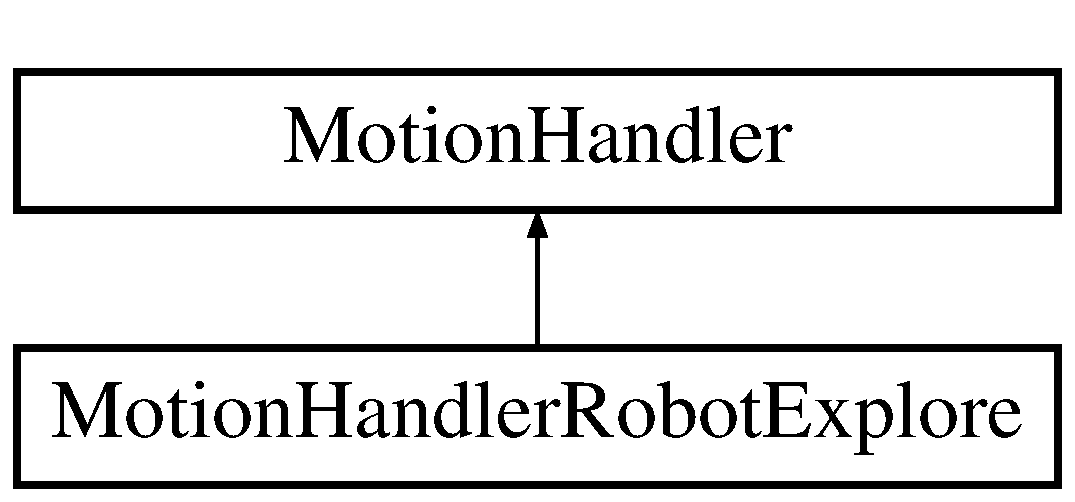
\includegraphics[height=2.000000cm]{class_motion_handler_robot_explore}
\end{center}
\end{figure}
\subsection*{Public Member Functions}
\begin{DoxyCompactItemize}
\item 
{\bfseries Motion\+Handler\+Robot\+Explore} (\hyperlink{class_arena_mobile_entity}{Arena\+Mobile\+Entity} $\ast$ent)\hypertarget{class_motion_handler_robot_explore_a5d62df9b7ffd800d4b35859ba1a72f3e}{}\label{class_motion_handler_robot_explore_a5d62df9b7ffd800d4b35859ba1a72f3e}

\item 
{\bfseries Motion\+Handler\+Robot\+Explore} (const \hyperlink{class_motion_handler_robot_explore}{Motion\+Handler\+Robot\+Explore} \&other)=default\hypertarget{class_motion_handler_robot_explore_ae82ba22271a4cf497d68f4bcd8c4b4e4}{}\label{class_motion_handler_robot_explore_ae82ba22271a4cf497d68f4bcd8c4b4e4}

\item 
\hyperlink{class_motion_handler_robot_explore}{Motion\+Handler\+Robot\+Explore} \& {\bfseries operator=} (const \hyperlink{class_motion_handler_robot_explore}{Motion\+Handler\+Robot\+Explore} \&other)=default\hypertarget{class_motion_handler_robot_explore_a4ee07340d788ea4fdc7de86b5f51da02}{}\label{class_motion_handler_robot_explore_a4ee07340d788ea4fdc7de86b5f51da02}

\item 
void \hyperlink{class_motion_handler_robot_explore_a88d0b13f1082475630d1955258aaa174}{Update\+Velocity} () override\hypertarget{class_motion_handler_robot_explore_a88d0b13f1082475630d1955258aaa174}{}\label{class_motion_handler_robot_explore_a88d0b13f1082475630d1955258aaa174}

\begin{DoxyCompactList}\small\item\em Update the speed and the pose angle according to the explore sensor readings.. \end{DoxyCompactList}\item 
void \hyperlink{class_motion_handler_robot_explore_aa52a668bd64c17b56dbd0be199cddc2c}{Increase\+Speed} () override\hypertarget{class_motion_handler_robot_explore_aa52a668bd64c17b56dbd0be199cddc2c}{}\label{class_motion_handler_robot_explore_aa52a668bd64c17b56dbd0be199cddc2c}

\begin{DoxyCompactList}\small\item\em Increase the overall speed of the entity by speed\+\_\+delta. \end{DoxyCompactList}\item 
void \hyperlink{class_motion_handler_robot_explore_a8898051b46761b8ba64468a3afa1bbca}{Decrease\+Speed} () override\hypertarget{class_motion_handler_robot_explore_a8898051b46761b8ba64468a3afa1bbca}{}\label{class_motion_handler_robot_explore_a8898051b46761b8ba64468a3afa1bbca}

\begin{DoxyCompactList}\small\item\em Decrease the overall speed of the entity by speed\+\_\+delta. \end{DoxyCompactList}\item 
void \hyperlink{class_motion_handler_robot_explore_a2641f1d587f28f454f0455f6ccc98c3f}{Turn\+Right} () override\hypertarget{class_motion_handler_robot_explore_a2641f1d587f28f454f0455f6ccc98c3f}{}\label{class_motion_handler_robot_explore_a2641f1d587f28f454f0455f6ccc98c3f}

\begin{DoxyCompactList}\small\item\em Turn the entity to the right by angle\+\_\+delta (in degrees?) \end{DoxyCompactList}\item 
void \hyperlink{class_motion_handler_robot_explore_a4abe8735e4f4d22757a544d075885402}{Turn\+Left} () override\hypertarget{class_motion_handler_robot_explore_a4abe8735e4f4d22757a544d075885402}{}\label{class_motion_handler_robot_explore_a4abe8735e4f4d22757a544d075885402}

\begin{DoxyCompactList}\small\item\em Turn the entity to the left by angle\+\_\+delta (in degrees?) \end{DoxyCompactList}\item 
void \hyperlink{class_motion_handler_robot_explore_a975326a8f0719b6feb48a7aa24afe4ea}{Stop} () override\hypertarget{class_motion_handler_robot_explore_a975326a8f0719b6feb48a7aa24afe4ea}{}\label{class_motion_handler_robot_explore_a975326a8f0719b6feb48a7aa24afe4ea}

\begin{DoxyCompactList}\small\item\em stop the entity to be at zero velocity. \end{DoxyCompactList}\end{DoxyCompactItemize}
\subsection*{Additional Inherited Members}


\subsection{Detailed Description}
Class managing a \hyperlink{class_robot}{Robot}\textquotesingle{}s and \hyperlink{class_light}{Light}\textquotesingle{}s speed and heading angle based on the explore sensor readings. 

The documentation for this class was generated from the following files\+:\begin{DoxyCompactItemize}
\item 
src/\hyperlink{motion__handler__robot__explore_8h}{motion\+\_\+handler\+\_\+robot\+\_\+explore.\+h}\item 
src/\hyperlink{motion__handler__robot__explore_8cc}{motion\+\_\+handler\+\_\+robot\+\_\+explore.\+cc}\end{DoxyCompactItemize}

\hypertarget{class_motion_handler_robot_love}{}\section{Motion\+Handler\+Robot\+Love Class Reference}
\label{class_motion_handler_robot_love}\index{Motion\+Handler\+Robot\+Love@{Motion\+Handler\+Robot\+Love}}


Class managing a \mbox{\hyperlink{class_robot}{Robot}}\textquotesingle{}s and \mbox{\hyperlink{class_light}{Light}}\textquotesingle{}s speed and heading angle based on the love sensor readings.  




{\ttfamily \#include $<$motion\+\_\+handler\+\_\+robot\+\_\+love.\+h$>$}

Inheritance diagram for Motion\+Handler\+Robot\+Love\+:\begin{figure}[H]
\begin{center}
\leavevmode
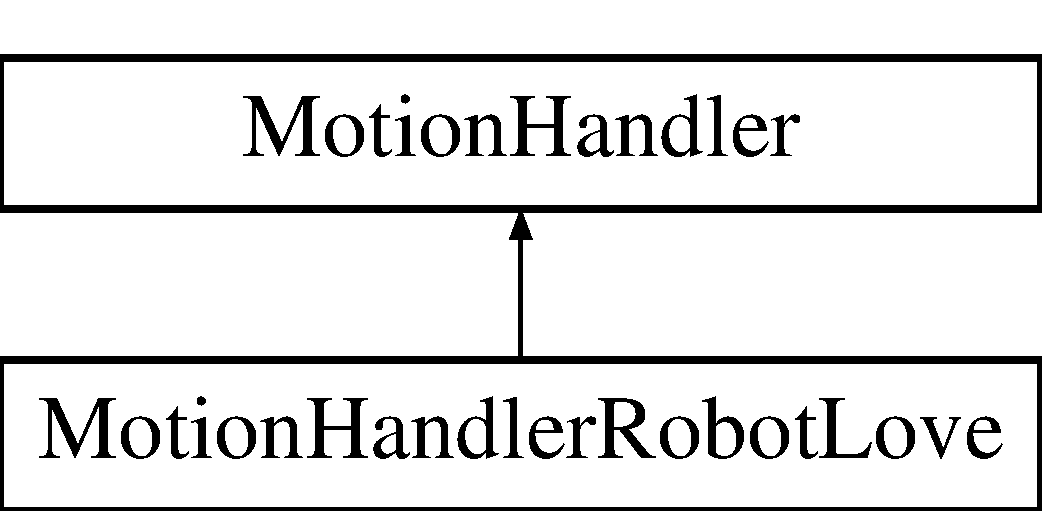
\includegraphics[height=2.000000cm]{class_motion_handler_robot_love}
\end{center}
\end{figure}
\subsection*{Public Member Functions}
\begin{DoxyCompactItemize}
\item 
\mbox{\Hypertarget{class_motion_handler_robot_love_aa2e0d7f03281a230f095d825ab2b35c6}\label{class_motion_handler_robot_love_aa2e0d7f03281a230f095d825ab2b35c6}} 
{\bfseries Motion\+Handler\+Robot\+Love} (\mbox{\hyperlink{class_arena_mobile_entity}{Arena\+Mobile\+Entity}} $\ast$ent)
\item 
\mbox{\Hypertarget{class_motion_handler_robot_love_a547d8a567954d2b82ef8e5f30f1c9515}\label{class_motion_handler_robot_love_a547d8a567954d2b82ef8e5f30f1c9515}} 
{\bfseries Motion\+Handler\+Robot\+Love} (const \mbox{\hyperlink{class_motion_handler_robot_love}{Motion\+Handler\+Robot\+Love}} \&other)=default
\item 
\mbox{\Hypertarget{class_motion_handler_robot_love_a5a281795ebc5df70d5529fc012bc4aa5}\label{class_motion_handler_robot_love_a5a281795ebc5df70d5529fc012bc4aa5}} 
\mbox{\hyperlink{class_motion_handler_robot_love}{Motion\+Handler\+Robot\+Love}} \& {\bfseries operator=} (const \mbox{\hyperlink{class_motion_handler_robot_love}{Motion\+Handler\+Robot\+Love}} \&other)=default
\item 
\mbox{\Hypertarget{class_motion_handler_robot_love_a3d4030e29ee33bbd4cddfc9850543615}\label{class_motion_handler_robot_love_a3d4030e29ee33bbd4cddfc9850543615}} 
void \mbox{\hyperlink{class_motion_handler_robot_love_a3d4030e29ee33bbd4cddfc9850543615}{Update\+Velocity}} () override
\begin{DoxyCompactList}\small\item\em Update the speed and the pose angle according to the sensor readings. \end{DoxyCompactList}\item 
\mbox{\Hypertarget{class_motion_handler_robot_love_ac4b0287075f1ec75e9b1bb776eb428f6}\label{class_motion_handler_robot_love_ac4b0287075f1ec75e9b1bb776eb428f6}} 
void \mbox{\hyperlink{class_motion_handler_robot_love_ac4b0287075f1ec75e9b1bb776eb428f6}{Increase\+Speed}} () override
\begin{DoxyCompactList}\small\item\em Increase the overall speed of the entity by speed\+\_\+delta. \end{DoxyCompactList}\item 
\mbox{\Hypertarget{class_motion_handler_robot_love_af64d850f198beaccdc9dad1a519c387c}\label{class_motion_handler_robot_love_af64d850f198beaccdc9dad1a519c387c}} 
void \mbox{\hyperlink{class_motion_handler_robot_love_af64d850f198beaccdc9dad1a519c387c}{Decrease\+Speed}} () override
\begin{DoxyCompactList}\small\item\em Decrease the overall speed of the entity by speed\+\_\+delta. \end{DoxyCompactList}\item 
\mbox{\Hypertarget{class_motion_handler_robot_love_aeff4a675940af2d42c6a8fd2a4519d66}\label{class_motion_handler_robot_love_aeff4a675940af2d42c6a8fd2a4519d66}} 
void \mbox{\hyperlink{class_motion_handler_robot_love_aeff4a675940af2d42c6a8fd2a4519d66}{Turn\+Right}} () override
\begin{DoxyCompactList}\small\item\em Turn the entity to the right by angle\+\_\+delta (in degrees?) \end{DoxyCompactList}\item 
\mbox{\Hypertarget{class_motion_handler_robot_love_a26b07483889261be22d5df90d2bdf81c}\label{class_motion_handler_robot_love_a26b07483889261be22d5df90d2bdf81c}} 
void \mbox{\hyperlink{class_motion_handler_robot_love_a26b07483889261be22d5df90d2bdf81c}{Turn\+Left}} () override
\begin{DoxyCompactList}\small\item\em Turn the entity to the left by angle\+\_\+delta (in degrees?) \end{DoxyCompactList}\item 
\mbox{\Hypertarget{class_motion_handler_robot_love_aaff39b4c62e5c46743bc65af94e9a09a}\label{class_motion_handler_robot_love_aaff39b4c62e5c46743bc65af94e9a09a}} 
void \mbox{\hyperlink{class_motion_handler_robot_love_aaff39b4c62e5c46743bc65af94e9a09a}{Stop}} () override
\begin{DoxyCompactList}\small\item\em stop the entity to be at zero velocity. \end{DoxyCompactList}\end{DoxyCompactItemize}
\subsection*{Additional Inherited Members}


\subsection{Detailed Description}
Class managing a \mbox{\hyperlink{class_robot}{Robot}}\textquotesingle{}s and \mbox{\hyperlink{class_light}{Light}}\textquotesingle{}s speed and heading angle based on the love sensor readings. 

The documentation for this class was generated from the following files\+:\begin{DoxyCompactItemize}
\item 
src/\mbox{\hyperlink{motion__handler__robot__love_8h}{motion\+\_\+handler\+\_\+robot\+\_\+love.\+h}}\item 
src/\mbox{\hyperlink{motion__handler__robot__love_8cc}{motion\+\_\+handler\+\_\+robot\+\_\+love.\+cc}}\end{DoxyCompactItemize}

\hypertarget{struct_pose}{}\section{Pose Struct Reference}
\label{struct_pose}\index{Pose@{Pose}}


A simple representation of the position/orientation of an entity within the \hyperlink{class_arena}{Arena}.  




{\ttfamily \#include $<$pose.\+h$>$}

\subsection*{Public Member Functions}
\begin{DoxyCompactItemize}
\item 
\hyperlink{struct_pose_a8a4171c8a6b09e37fb011997da9ea2ad}{Pose} ()\hypertarget{struct_pose_a8a4171c8a6b09e37fb011997da9ea2ad}{}\label{struct_pose_a8a4171c8a6b09e37fb011997da9ea2ad}

\begin{DoxyCompactList}\small\item\em Default constructor. Initialize the pose to (0,0,0) \end{DoxyCompactList}\item 
\hyperlink{struct_pose_ac947d7046547d883f782ab2408cb80ed}{Pose} (double in\+\_\+x, double in\+\_\+y)
\begin{DoxyCompactList}\small\item\em Constructor. \end{DoxyCompactList}\item 
{\bfseries Pose} (double in\+\_\+x, double in\+\_\+y, double in\+\_\+theta)\hypertarget{struct_pose_a6ebb8a1510c5915fa1dbec0f7ba0ad1c}{}\label{struct_pose_a6ebb8a1510c5915fa1dbec0f7ba0ad1c}

\item 
\hyperlink{struct_pose}{Pose} \& \hyperlink{struct_pose_aec0a9478daefa358aa2f1873cbaf0271}{operator=} (const \hyperlink{struct_pose}{Pose} \&other)=default
\begin{DoxyCompactList}\small\item\em Default assignment operator. Simply copies the (x,y) values of another \hyperlink{struct_pose}{Pose}. \end{DoxyCompactList}\end{DoxyCompactItemize}
\subsection*{Public Attributes}
\begin{DoxyCompactItemize}
\item 
double {\bfseries x} \{0\}\hypertarget{struct_pose_a0061c7789df90f593ab95118cbef387f}{}\label{struct_pose_a0061c7789df90f593ab95118cbef387f}

\item 
double {\bfseries y} \{0\}\hypertarget{struct_pose_a6280216efe0840a7a55f025ad04e3b3d}{}\label{struct_pose_a6280216efe0840a7a55f025ad04e3b3d}

\item 
double {\bfseries theta} \{0.\+0\}\hypertarget{struct_pose_a25709c116282114c9f512b205f3f1133}{}\label{struct_pose_a25709c116282114c9f512b205f3f1133}

\end{DoxyCompactItemize}


\subsection{Detailed Description}
A simple representation of the position/orientation of an entity within the \hyperlink{class_arena}{Arena}. 

N\+O\+TE\+: Origin (0,0) is at the upper left corner of the \hyperlink{class_arena}{Arena}. 

\subsection{Constructor \& Destructor Documentation}
\index{Pose@{Pose}!Pose@{Pose}}
\index{Pose@{Pose}!Pose@{Pose}}
\subsubsection[{\texorpdfstring{Pose(double in\+\_\+x, double in\+\_\+y)}{Pose(double in_x, double in_y)}}]{\setlength{\rightskip}{0pt plus 5cm}Pose\+::\+Pose (
\begin{DoxyParamCaption}
\item[{double}]{in\+\_\+x, }
\item[{double}]{in\+\_\+y}
\end{DoxyParamCaption}
)\hspace{0.3cm}{\ttfamily [inline]}}\hypertarget{struct_pose_ac947d7046547d883f782ab2408cb80ed}{}\label{struct_pose_ac947d7046547d883f782ab2408cb80ed}


Constructor. 


\begin{DoxyParams}{Parameters}
{\em in\+\_\+x} & The X component of the \hyperlink{struct_pose}{Pose}. \\
\hline
{\em in\+\_\+y} & The Y component of the \hyperlink{struct_pose}{Pose}. \\
\hline
\end{DoxyParams}


\subsection{Member Function Documentation}
\index{Pose@{Pose}!operator=@{operator=}}
\index{operator=@{operator=}!Pose@{Pose}}
\subsubsection[{\texorpdfstring{operator=(const Pose \&other)=default}{operator=(const Pose &other)=default}}]{\setlength{\rightskip}{0pt plus 5cm}{\bf Pose}\& Pose\+::operator= (
\begin{DoxyParamCaption}
\item[{const {\bf Pose} \&}]{other}
\end{DoxyParamCaption}
)\hspace{0.3cm}{\ttfamily [default]}}\hypertarget{struct_pose_aec0a9478daefa358aa2f1873cbaf0271}{}\label{struct_pose_aec0a9478daefa358aa2f1873cbaf0271}


Default assignment operator. Simply copies the (x,y) values of another \hyperlink{struct_pose}{Pose}. 


\begin{DoxyParams}{Parameters}
{\em other} & The \hyperlink{struct_pose}{Pose} object to copy from.\\
\hline
\end{DoxyParams}
\begin{DoxyReturn}{Returns}
The left-\/hand-\/side \hyperlink{struct_pose}{Pose} object that is now identical (in value) to {\ttfamily other}. 
\end{DoxyReturn}


The documentation for this struct was generated from the following file\+:\begin{DoxyCompactItemize}
\item 
src/\hyperlink{pose_8h}{pose.\+h}\end{DoxyCompactItemize}

\hypertarget{struct_rgb_color}{}\section{Rgb\+Color Struct Reference}
\label{struct_rgb_color}\index{Rgb\+Color@{Rgb\+Color}}


Struct representing a rgb\+\_\+color.  




{\ttfamily \#include $<$rgb\+\_\+color.\+h$>$}

\subsection*{Public Member Functions}
\begin{DoxyCompactItemize}
\item 
\mbox{\hyperlink{struct_rgb_color_a264da0270aca412d62197e046b71b08e}{Rgb\+Color}} ()
\begin{DoxyCompactList}\small\item\em Default constructor. \end{DoxyCompactList}\item 
\mbox{\hyperlink{struct_rgb_color_a61e213533bfff019aebd27f991688222}{Rgb\+Color}} (int r\+\_\+in, int g\+\_\+in, int b\+\_\+in)
\begin{DoxyCompactList}\small\item\em Constructor for Rgb\+\_\+\+Color. \end{DoxyCompactList}\item 
\mbox{\Hypertarget{struct_rgb_color_a57fcd9161e0ee6a38e707c5002db55b8}\label{struct_rgb_color_a57fcd9161e0ee6a38e707c5002db55b8}} 
void {\bfseries Set} (Rgb\+Color\+Enum value)
\end{DoxyCompactItemize}
\subsection*{Public Attributes}
\begin{DoxyCompactItemize}
\item 
\mbox{\Hypertarget{struct_rgb_color_aa6c2fac108029c79f7cc96fb6d34717f}\label{struct_rgb_color_aa6c2fac108029c79f7cc96fb6d34717f}} 
int {\bfseries r} \{0\}
\item 
\mbox{\Hypertarget{struct_rgb_color_afbc54745bd4ed7ede168e31922143eff}\label{struct_rgb_color_afbc54745bd4ed7ede168e31922143eff}} 
int {\bfseries g} \{0\}
\item 
\mbox{\Hypertarget{struct_rgb_color_af1ba4837230cfc3b0f31454ccdb03df6}\label{struct_rgb_color_af1ba4837230cfc3b0f31454ccdb03df6}} 
int {\bfseries b} \{0\}
\end{DoxyCompactItemize}


\subsection{Detailed Description}
Struct representing a rgb\+\_\+color. 

Internally uses R\+G\+BA values to represent the rgb\+\_\+color. 

\subsection{Constructor \& Destructor Documentation}
\mbox{\Hypertarget{struct_rgb_color_a264da0270aca412d62197e046b71b08e}\label{struct_rgb_color_a264da0270aca412d62197e046b71b08e}} 
\index{Rgb\+Color@{Rgb\+Color}!Rgb\+Color@{Rgb\+Color}}
\index{Rgb\+Color@{Rgb\+Color}!Rgb\+Color@{Rgb\+Color}}
\subsubsection{\texorpdfstring{Rgb\+Color()}{RgbColor()}\hspace{0.1cm}{\footnotesize\ttfamily [1/2]}}
{\footnotesize\ttfamily Rgb\+Color\+::\+Rgb\+Color (\begin{DoxyParamCaption}{ }\end{DoxyParamCaption})\hspace{0.3cm}{\ttfamily [inline]}}



Default constructor. 

Initialize R\+GB all to 0 (k\+White). \mbox{\Hypertarget{struct_rgb_color_a61e213533bfff019aebd27f991688222}\label{struct_rgb_color_a61e213533bfff019aebd27f991688222}} 
\index{Rgb\+Color@{Rgb\+Color}!Rgb\+Color@{Rgb\+Color}}
\index{Rgb\+Color@{Rgb\+Color}!Rgb\+Color@{Rgb\+Color}}
\subsubsection{\texorpdfstring{Rgb\+Color()}{RgbColor()}\hspace{0.1cm}{\footnotesize\ttfamily [2/2]}}
{\footnotesize\ttfamily Rgb\+Color\+::\+Rgb\+Color (\begin{DoxyParamCaption}\item[{int}]{r\+\_\+in,  }\item[{int}]{g\+\_\+in,  }\item[{int}]{b\+\_\+in }\end{DoxyParamCaption})\hspace{0.3cm}{\ttfamily [inline]}}



Constructor for Rgb\+\_\+\+Color. 


\begin{DoxyParams}{Parameters}
{\em r\+\_\+in} & The R component of the rgb\+\_\+color. \\
\hline
{\em g\+\_\+in} & The G component of the rgb\+\_\+color. \\
\hline
{\em b\+\_\+in} & The B component of the rgb\+\_\+color. \\
\hline
\end{DoxyParams}


The documentation for this struct was generated from the following files\+:\begin{DoxyCompactItemize}
\item 
src/\mbox{\hyperlink{rgb__color_8h}{rgb\+\_\+color.\+h}}\item 
src/\mbox{\hyperlink{rgb__color_8cc}{rgb\+\_\+color.\+cc}}\end{DoxyCompactItemize}

\hypertarget{class_robot}{}\section{Robot Class Reference}
\label{class_robot}\index{Robot@{Robot}}


Class representing a robot within the arena.  




{\ttfamily \#include $<$robot.\+h$>$}

Inheritance diagram for Robot\+:\begin{figure}[H]
\begin{center}
\leavevmode
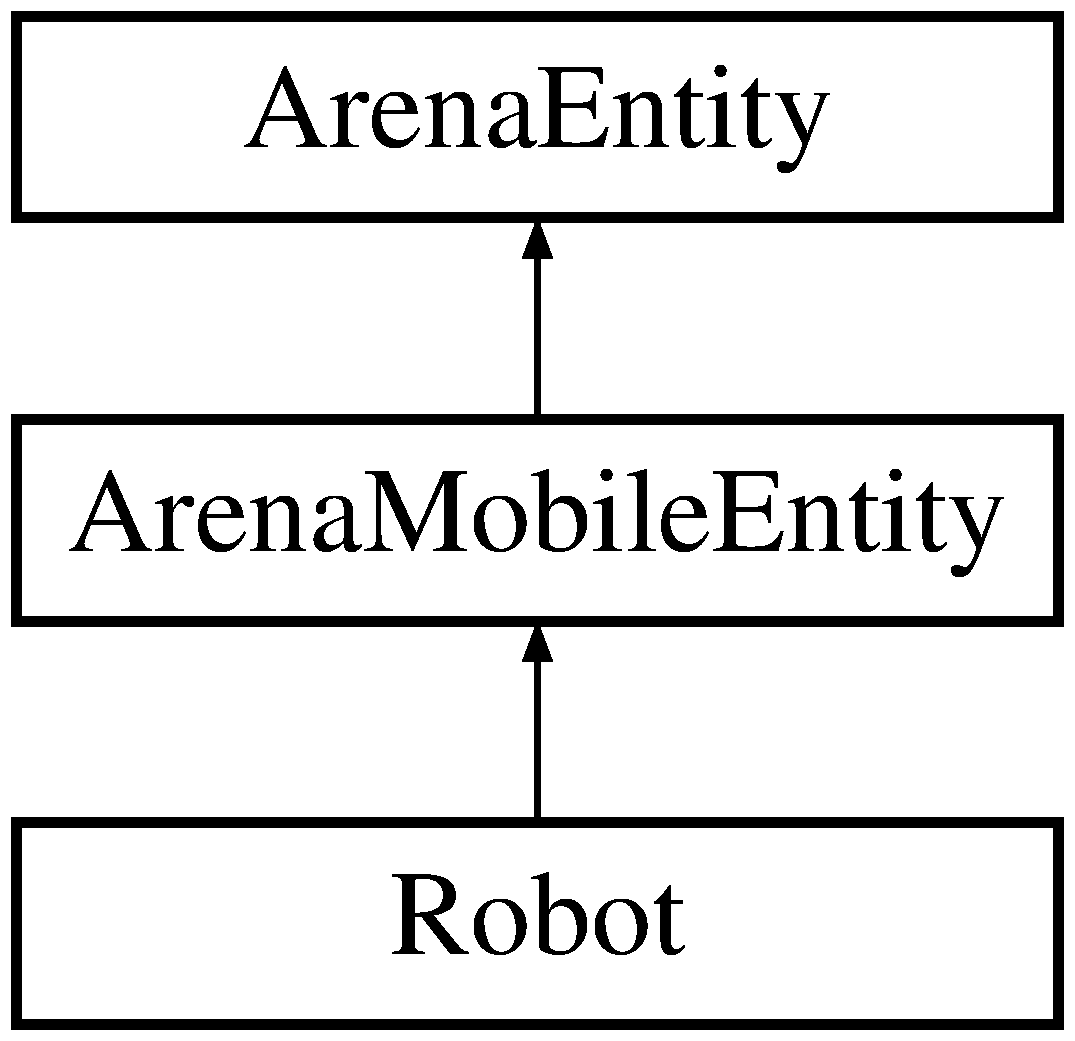
\includegraphics[height=3.000000cm]{class_robot}
\end{center}
\end{figure}
\subsection*{Public Member Functions}
\begin{DoxyCompactItemize}
\item 
\hyperlink{class_robot_a3475f306d3a9b7090e31a12399260055}{Robot} (Robot\+Type rt)\hypertarget{class_robot_a3475f306d3a9b7090e31a12399260055}{}\label{class_robot_a3475f306d3a9b7090e31a12399260055}

\begin{DoxyCompactList}\small\item\em Constructor using initialization values from \hyperlink{params_8h}{params.\+h}. \end{DoxyCompactList}\item 
\hyperlink{class_robot_a4fd835c7c44337d31d9fd09921d29908}{Robot} (const \hyperlink{class_robot}{Robot} \&)=default\hypertarget{class_robot_a4fd835c7c44337d31d9fd09921d29908}{}\label{class_robot_a4fd835c7c44337d31d9fd09921d29908}

\begin{DoxyCompactList}\small\item\em Reset the \hyperlink{class_robot}{Robot} to a newly constructed state (needed for reset button to work in G\+UI). \end{DoxyCompactList}\item 
\hyperlink{class_robot}{Robot} \& {\bfseries operator=} (const \hyperlink{class_robot}{Robot} \&other)=default\hypertarget{class_robot_a69f171c4965ac4523cd95e2191405d37}{}\label{class_robot_a69f171c4965ac4523cd95e2191405d37}

\item 
void \hyperlink{class_robot_af597fd14927d2cd5308ded62f4e54e29}{Reset} () override\hypertarget{class_robot_af597fd14927d2cd5308ded62f4e54e29}{}\label{class_robot_af597fd14927d2cd5308ded62f4e54e29}

\begin{DoxyCompactList}\small\item\em Reset entity to a newly constructed state. \end{DoxyCompactList}\item 
void \hyperlink{class_robot_ae790462f8782efcfd26082eedec30ed5}{Timestep\+Update} (unsigned int dt) override
\begin{DoxyCompactList}\small\item\em Update the \hyperlink{class_robot}{Robot}\textquotesingle{}s position and velocity after the specified duration has passed. \end{DoxyCompactList}\item 
void \hyperlink{class_robot_a4fc6b01fec869b559197d8e4b9686249}{Handle\+Collision} (Entity\+Type object\+\_\+type, \hyperlink{class_arena_entity}{Arena\+Entity} $\ast$object=N\+U\+LL) override\hypertarget{class_robot_a4fc6b01fec869b559197d8e4b9686249}{}\label{class_robot_a4fc6b01fec869b559197d8e4b9686249}

\begin{DoxyCompactList}\small\item\em Handles the collision by setting the sensor to activated. \end{DoxyCompactList}\item 
std\+::string \hyperlink{class_robot_a3f77c13705b8f60480d21d8d936dc39e}{get\+\_\+name} () const override\hypertarget{class_robot_a3f77c13705b8f60480d21d8d936dc39e}{}\label{class_robot_a3f77c13705b8f60480d21d8d936dc39e}

\begin{DoxyCompactList}\small\item\em Get the name of the \hyperlink{class_robot}{Robot} for visualization and for debugging. \end{DoxyCompactList}\item 
void \hyperlink{class_robot_ae4647cccd002ca13659017e634237ead}{Increase\+Speed} ()\hypertarget{class_robot_ae4647cccd002ca13659017e634237ead}{}\label{class_robot_ae4647cccd002ca13659017e634237ead}

\begin{DoxyCompactList}\small\item\em Command that comes from the controller, then is passed to handler. \end{DoxyCompactList}\item 
void \hyperlink{class_robot_a94afa6f63eb22667261c07933faae481}{Decrease\+Speed} ()\hypertarget{class_robot_a94afa6f63eb22667261c07933faae481}{}\label{class_robot_a94afa6f63eb22667261c07933faae481}

\begin{DoxyCompactList}\small\item\em Command that comes from the controller, then is passed to handler. \end{DoxyCompactList}\item 
void \hyperlink{class_robot_a12b5883779f682c66e71bc54b6539694}{Turn\+Right} ()\hypertarget{class_robot_a12b5883779f682c66e71bc54b6539694}{}\label{class_robot_a12b5883779f682c66e71bc54b6539694}

\begin{DoxyCompactList}\small\item\em Command that comes from the controller, then is passed to handler. \end{DoxyCompactList}\item 
void \hyperlink{class_robot_ad864d21d997dbadf55f997c2f0143d41}{Turn\+Left} ()\hypertarget{class_robot_ad864d21d997dbadf55f997c2f0143d41}{}\label{class_robot_ad864d21d997dbadf55f997c2f0143d41}

\begin{DoxyCompactList}\small\item\em Command that comes from the controller, then is passed to handler. \end{DoxyCompactList}\item 
void \hyperlink{class_robot_ae0a3474ce96a7edee32f1b6597308d80}{lose\+\_\+\+A\+\_\+\+Life} ()\hypertarget{class_robot_ae0a3474ce96a7edee32f1b6597308d80}{}\label{class_robot_ae0a3474ce96a7edee32f1b6597308d80}

\begin{DoxyCompactList}\small\item\em Function called when robot loose a single life. \end{DoxyCompactList}\item 
void \hyperlink{class_robot_ad71cb8a7785ec61e938b62d1eb85c70e}{Increment\+Robot\+Time} ()\hypertarget{class_robot_ad71cb8a7785ec61e938b62d1eb85c70e}{}\label{class_robot_ad71cb8a7785ec61e938b62d1eb85c70e}

\begin{DoxyCompactList}\small\item\em Function to increment the robots time to track hunger. \end{DoxyCompactList}\item 
int {\bfseries get\+\_\+lives} () const \hypertarget{class_robot_a201302eeb10756e9f9a54de414efef08}{}\label{class_robot_a201302eeb10756e9f9a54de414efef08}

\item 
void {\bfseries set\+\_\+lives} (int l)\hypertarget{class_robot_a8823c73b258afe8cf8ef276e8f2f9aab}{}\label{class_robot_a8823c73b258afe8cf8ef276e8f2f9aab}

\item 
\hyperlink{class_motion_handler}{Motion\+Handler} $\ast$ {\bfseries get\+\_\+motion\+\_\+handler} ()\hypertarget{class_robot_a80b6c7f15493d4b5c608d185b9a116ce}{}\label{class_robot_a80b6c7f15493d4b5c608d185b9a116ce}

\item 
\hyperlink{class_motion_behavior_differential}{Motion\+Behavior\+Differential} {\bfseries get\+\_\+motion\+\_\+behavior} ()\hypertarget{class_robot_ab45bf3c6fdafcd14cdbdb2a8e3f558b8}{}\label{class_robot_ab45bf3c6fdafcd14cdbdb2a8e3f558b8}

\item 
\hyperlink{class_light_sensor}{Light\+Sensor} $\ast$ {\bfseries get\+\_\+left\+\_\+light\+\_\+sensor} ()\hypertarget{class_robot_ac2e00bdd8bfac97d1bd89c86ee0fd727}{}\label{class_robot_ac2e00bdd8bfac97d1bd89c86ee0fd727}

\item 
\hyperlink{class_light_sensor}{Light\+Sensor} $\ast$ {\bfseries get\+\_\+right\+\_\+light\+\_\+sensor} ()\hypertarget{class_robot_aff66784b080f5d7329a8f45d679d1b60}{}\label{class_robot_aff66784b080f5d7329a8f45d679d1b60}

\item 
\hyperlink{class_food_sensor}{Food\+Sensor} $\ast$ {\bfseries get\+\_\+right\+\_\+food\+\_\+sensor} ()\hypertarget{class_robot_acdf59a9f9124f4d8a910a2fa85e4d7c3}{}\label{class_robot_acdf59a9f9124f4d8a910a2fa85e4d7c3}

\item 
\hyperlink{class_food_sensor}{Food\+Sensor} $\ast$ {\bfseries get\+\_\+left\+\_\+food\+\_\+sensor} ()\hypertarget{class_robot_a6bde50502517a623c309dbfbef546063}{}\label{class_robot_a6bde50502517a623c309dbfbef546063}

\item 
void {\bfseries set\+\_\+robot\+\_\+type} (Robot\+Type rt)\hypertarget{class_robot_ad811b955d24c95ebb16f0a2c185876a9}{}\label{class_robot_ad811b955d24c95ebb16f0a2c185876a9}

\item 
Robot\+Type {\bfseries get\+\_\+robot\+\_\+type} ()\hypertarget{class_robot_a1463b5699ff9a30a76768f7570b43b0d}{}\label{class_robot_a1463b5699ff9a30a76768f7570b43b0d}

\item 
void {\bfseries set\+\_\+hunger} (bool hunger)\hypertarget{class_robot_a3acf3a0f65d23859d7991667b09d28ef}{}\label{class_robot_a3acf3a0f65d23859d7991667b09d28ef}

\item 
bool {\bfseries get\+\_\+hunger} ()\hypertarget{class_robot_aacdc924197b130a93046168cc31933a8}{}\label{class_robot_aacdc924197b130a93046168cc31933a8}

\item 
int {\bfseries get\+\_\+robot\+\_\+time} ()\hypertarget{class_robot_ae8f5051655c730486561e43be5602ca7}{}\label{class_robot_ae8f5051655c730486561e43be5602ca7}

\item 
void {\bfseries Restart\+Robot\+Time} ()\hypertarget{class_robot_a80dc608c5bf63c6d3b814a9f36fde462}{}\label{class_robot_a80dc608c5bf63c6d3b814a9f36fde462}

\item 
void {\bfseries Update\+Sensor\+Poses} ()\hypertarget{class_robot_a1227689786b8842a3cd14204a98c891d}{}\label{class_robot_a1227689786b8842a3cd14204a98c891d}

\end{DoxyCompactItemize}
\subsection*{Additional Inherited Members}


\subsection{Detailed Description}
Class representing a robot within the arena. 

Robots are composed of a motion handler, motion behavior, and touch sensor. These classes interact to maintain the pose (position and heading) of the robot. At each time step, the wheel velocities are used to calculate the next pose of the robot. The handler manages the pose and user requests. The behavior calculates the new pose based on wheel velocities.

Robots can be controlled through keypress, which modify wheel velocities.

The touch sensor is activated when the robot collides with an object. The heading is modified after a collision to move the robot away from the other object. 

\subsection{Member Function Documentation}
\index{Robot@{Robot}!Timestep\+Update@{Timestep\+Update}}
\index{Timestep\+Update@{Timestep\+Update}!Robot@{Robot}}
\subsubsection[{\texorpdfstring{Timestep\+Update(unsigned int dt) override}{TimestepUpdate(unsigned int dt) override}}]{\setlength{\rightskip}{0pt plus 5cm}void Robot\+::\+Timestep\+Update (
\begin{DoxyParamCaption}
\item[{unsigned int}]{dt}
\end{DoxyParamCaption}
)\hspace{0.3cm}{\ttfamily [override]}}\hypertarget{class_robot_ae790462f8782efcfd26082eedec30ed5}{}\label{class_robot_ae790462f8782efcfd26082eedec30ed5}


Update the \hyperlink{class_robot}{Robot}\textquotesingle{}s position and velocity after the specified duration has passed. 


\begin{DoxyParams}{Parameters}
{\em dt} & The \# of timesteps that have elapsed since the last update. \\
\hline
\end{DoxyParams}


The documentation for this class was generated from the following files\+:\begin{DoxyCompactItemize}
\item 
src/\hyperlink{robot_8h}{robot.\+h}\item 
src/\hyperlink{robot_8cc}{robot.\+cc}\end{DoxyCompactItemize}

\hypertarget{class_sensor}{}\section{Sensor Class Reference}
\label{class_sensor}\index{Sensor@{Sensor}}
Inheritance diagram for Sensor\+:\begin{figure}[H]
\begin{center}
\leavevmode
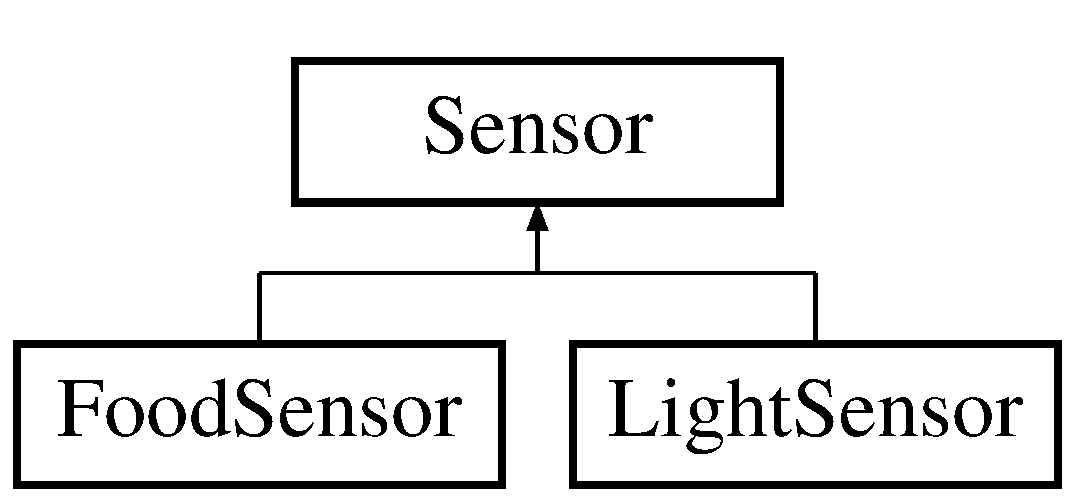
\includegraphics[height=2.000000cm]{class_sensor}
\end{center}
\end{figure}
\subsection*{Public Member Functions}
\begin{DoxyCompactItemize}
\item 
{\bfseries Sensor} (\hyperlink{class_arena_mobile_entity}{Arena\+Mobile\+Entity} $\ast$ent)\hypertarget{class_sensor_a13c4b3a00db6e21e2ac33647440fdc37}{}\label{class_sensor_a13c4b3a00db6e21e2ac33647440fdc37}

\item 
{\bfseries Sensor} (const \hyperlink{class_sensor}{Sensor} \&)=default\hypertarget{class_sensor_ac1d81bc5c639eeafed38d69e40dc07b8}{}\label{class_sensor_ac1d81bc5c639eeafed38d69e40dc07b8}

\item 
\hyperlink{class_sensor}{Sensor} \& {\bfseries operator=} (const \hyperlink{class_sensor}{Sensor} \&other)=default\hypertarget{class_sensor_a48b21cd29fa3f183a2fb9e6447de2219}{}\label{class_sensor_a48b21cd29fa3f183a2fb9e6447de2219}

\item 
virtual void {\bfseries update} (\hyperlink{common_8h_a2e3484535ee610c8e19e9859563abe48}{\+\_\+\+\_\+unused} std\+::vector$<$ class \hyperlink{class_arena_entity}{Arena\+Entity} $\ast$ $>$ stimili)\hypertarget{class_sensor_a152c11dc8df6982d0fad5b2082055e78}{}\label{class_sensor_a152c11dc8df6982d0fad5b2082055e78}

\item 
virtual void {\bfseries Reset} ()\hypertarget{class_sensor_a5e6ad1aa7b2c48e59851e03404dacbde}{}\label{class_sensor_a5e6ad1aa7b2c48e59851e03404dacbde}

\item 
void {\bfseries set\+\_\+reading} (int num)\hypertarget{class_sensor_a3ee42616cfe5e55c1efa2a4fd6761a44}{}\label{class_sensor_a3ee42616cfe5e55c1efa2a4fd6761a44}

\item 
int {\bfseries get\+\_\+reading} ()\hypertarget{class_sensor_ae574c5b7e58bdbbc47c0d83a7561fa19}{}\label{class_sensor_ae574c5b7e58bdbbc47c0d83a7561fa19}

\item 
void {\bfseries set\+\_\+pose} (\hyperlink{struct_pose}{Pose} p)\hypertarget{class_sensor_a877b65abc60821f62fe16771923fba38}{}\label{class_sensor_a877b65abc60821f62fe16771923fba38}

\item 
\hyperlink{struct_pose}{Pose} {\bfseries get\+\_\+pose} ()\hypertarget{class_sensor_afa533b8d8bb5f3787682ffc5ab8c989c}{}\label{class_sensor_afa533b8d8bb5f3787682ffc5ab8c989c}

\item 
void {\bfseries sensor\+\_\+robot\+\_\+location} (double angle)\hypertarget{class_sensor_a97e17a4d4b5fb30bf81d4ad6ee363715}{}\label{class_sensor_a97e17a4d4b5fb30bf81d4ad6ee363715}

\item 
const \hyperlink{struct_rgb_color}{Rgb\+Color} \& {\bfseries get\+\_\+color} () const \hypertarget{class_sensor_af5c275ceac411cfcc0903d6d837ed3e7}{}\label{class_sensor_af5c275ceac411cfcc0903d6d837ed3e7}

\item 
void {\bfseries set\+\_\+color} (const \hyperlink{struct_rgb_color}{Rgb\+Color} \&color)\hypertarget{class_sensor_a4c7c83edd18efc4a93d3fda798dbceec}{}\label{class_sensor_a4c7c83edd18efc4a93d3fda798dbceec}

\item 
void \hyperlink{class_sensor_aa38343db9a4da55dde95cb2579204b06}{set\+\_\+position} (const double inx, const double iny)\hypertarget{class_sensor_aa38343db9a4da55dde95cb2579204b06}{}\label{class_sensor_aa38343db9a4da55dde95cb2579204b06}

\begin{DoxyCompactList}\small\item\em Setter method for position within entity pose variable. \end{DoxyCompactList}\item 
void {\bfseries set\+\_\+heading} (const double t)\hypertarget{class_sensor_a95e911a62cef5adfbb0a8ee395cfa881}{}\label{class_sensor_a95e911a62cef5adfbb0a8ee395cfa881}

\item 
void \hyperlink{class_sensor_ad93b67ee775232e4b6e939fd043f0b84}{Relative\+Change\+Heading} (const double delta)
\begin{DoxyCompactList}\small\item\em Setter for heading within pose, but change is relative to current value. \end{DoxyCompactList}\item 
void {\bfseries change\+\_\+sensor\+\_\+sensitivity} (double ss)\hypertarget{class_sensor_a52e3dc66b6aeee78893d08a9d4511fae}{}\label{class_sensor_a52e3dc66b6aeee78893d08a9d4511fae}

\end{DoxyCompactItemize}
\subsection*{Protected Attributes}
\begin{DoxyCompactItemize}
\item 
\hyperlink{class_arena_mobile_entity}{Arena\+Mobile\+Entity} $\ast$ {\bfseries entity\+\_\+}\hypertarget{class_sensor_a03559676893c5d485ba8122d5aeb9bd4}{}\label{class_sensor_a03559676893c5d485ba8122d5aeb9bd4}

\item 
double {\bfseries sensor\+\_\+sensitivity} \{1.\+02\}\hypertarget{class_sensor_a090df848b7270a17ea41a0a28816515b}{}\label{class_sensor_a090df848b7270a17ea41a0a28816515b}

\end{DoxyCompactItemize}


\subsection{Member Function Documentation}
\index{Sensor@{Sensor}!Relative\+Change\+Heading@{Relative\+Change\+Heading}}
\index{Relative\+Change\+Heading@{Relative\+Change\+Heading}!Sensor@{Sensor}}
\subsubsection[{\texorpdfstring{Relative\+Change\+Heading(const double delta)}{RelativeChangeHeading(const double delta)}}]{\setlength{\rightskip}{0pt plus 5cm}void Sensor\+::\+Relative\+Change\+Heading (
\begin{DoxyParamCaption}
\item[{const double}]{delta}
\end{DoxyParamCaption}
)\hspace{0.3cm}{\ttfamily [inline]}}\hypertarget{class_sensor_ad93b67ee775232e4b6e939fd043f0b84}{}\label{class_sensor_ad93b67ee775232e4b6e939fd043f0b84}


Setter for heading within pose, but change is relative to current value. 


\begin{DoxyParams}[1]{Parameters}
\mbox{\tt in}  & {\em delta} & by which to modify current heading. Can be positive or negative. \\
\hline
\end{DoxyParams}


The documentation for this class was generated from the following file\+:\begin{DoxyCompactItemize}
\item 
src/\hyperlink{sensor_8h}{sensor.\+h}\end{DoxyCompactItemize}

\hypertarget{class_sensor_touch}{}\section{Sensor\+Touch Class Reference}
\label{class_sensor_touch}\index{Sensor\+Touch@{Sensor\+Touch}}


Class representing a touch sensor.  




{\ttfamily \#include $<$sensor\+\_\+touch.\+h$>$}

\subsection*{Public Member Functions}
\begin{DoxyCompactItemize}
\item 
\hyperlink{class_sensor_touch_ab8e0dc693ec2fbc1aa5ff25ee2bfdb19}{Sensor\+Touch} ()\hypertarget{class_sensor_touch_ab8e0dc693ec2fbc1aa5ff25ee2bfdb19}{}\label{class_sensor_touch_ab8e0dc693ec2fbc1aa5ff25ee2bfdb19}

\begin{DoxyCompactList}\small\item\em Constructor. \end{DoxyCompactList}\item 
const \hyperlink{struct_pose}{Pose} \& \hyperlink{class_sensor_touch_a9f56fd943758125611863ce2bc0d9365}{get\+\_\+point\+\_\+of\+\_\+contact} ()
\begin{DoxyCompactList}\small\item\em Getter method for the point of contact. \end{DoxyCompactList}\item 
void \hyperlink{class_sensor_touch_a2ef6d89a8e763e21f82e03a3033a490f}{set\+\_\+point\+\_\+of\+\_\+contact} (const \hyperlink{struct_pose}{Pose} \&p)
\begin{DoxyCompactList}\small\item\em Setter method for the point of contact. \end{DoxyCompactList}\item 
bool \hyperlink{class_sensor_touch_a6a2f77ea46d008f4a058bfb24db742e0}{get\+\_\+output} () const \hypertarget{class_sensor_touch_a6a2f77ea46d008f4a058bfb24db742e0}{}\label{class_sensor_touch_a6a2f77ea46d008f4a058bfb24db742e0}

\begin{DoxyCompactList}\small\item\em Getter for output, which is true when collision occurs. \end{DoxyCompactList}\item 
void \hyperlink{class_sensor_touch_a1980b126f7c6d0e6bdf75f1bb59fe5c2}{Handle\+Collision} (\hyperlink{common_8h_a2e3484535ee610c8e19e9859563abe48}{\+\_\+\+\_\+unused} Entity\+Type object\+\_\+type, \hyperlink{common_8h_a2e3484535ee610c8e19e9859563abe48}{\+\_\+\+\_\+unused} \hyperlink{class_arena_entity}{Arena\+Entity} $\ast$object)\hypertarget{class_sensor_touch_a1980b126f7c6d0e6bdf75f1bb59fe5c2}{}\label{class_sensor_touch_a1980b126f7c6d0e6bdf75f1bb59fe5c2}

\begin{DoxyCompactList}\small\item\em Modify heading to move away from collision. \end{DoxyCompactList}\item 
void \hyperlink{class_sensor_touch_ad0054916c97844a51052e5dee63f68b9}{Reset} ()\hypertarget{class_sensor_touch_ad0054916c97844a51052e5dee63f68b9}{}\label{class_sensor_touch_ad0054916c97844a51052e5dee63f68b9}

\begin{DoxyCompactList}\small\item\em Reset the sensor. \end{DoxyCompactList}\end{DoxyCompactItemize}


\subsection{Detailed Description}
Class representing a touch sensor. 

Touch or \char`\"{}bump\char`\"{} sensors are \char`\"{}active\char`\"{} when pressed. For our purposes, imagine a series of bump sensors around the perimeter of an entity. A collision will activate the sensor at a particular point of contact, which translates to an angle of contact.

\hyperlink{class_sensor_touch}{Sensor\+Touch} can be observed for collision events. 

\subsection{Member Function Documentation}
\index{Sensor\+Touch@{Sensor\+Touch}!get\+\_\+point\+\_\+of\+\_\+contact@{get\+\_\+point\+\_\+of\+\_\+contact}}
\index{get\+\_\+point\+\_\+of\+\_\+contact@{get\+\_\+point\+\_\+of\+\_\+contact}!Sensor\+Touch@{Sensor\+Touch}}
\subsubsection[{\texorpdfstring{get\+\_\+point\+\_\+of\+\_\+contact()}{get_point_of_contact()}}]{\setlength{\rightskip}{0pt plus 5cm}const {\bf Pose}\& Sensor\+Touch\+::get\+\_\+point\+\_\+of\+\_\+contact (
\begin{DoxyParamCaption}
{}
\end{DoxyParamCaption}
)\hspace{0.3cm}{\ttfamily [inline]}}\hypertarget{class_sensor_touch_a9f56fd943758125611863ce2bc0d9365}{}\label{class_sensor_touch_a9f56fd943758125611863ce2bc0d9365}


Getter method for the point of contact. 

Should only be called when the sensor is activated.

\begin{DoxyReturn}{Returns}
The latest point of contact. 
\end{DoxyReturn}
\index{Sensor\+Touch@{Sensor\+Touch}!set\+\_\+point\+\_\+of\+\_\+contact@{set\+\_\+point\+\_\+of\+\_\+contact}}
\index{set\+\_\+point\+\_\+of\+\_\+contact@{set\+\_\+point\+\_\+of\+\_\+contact}!Sensor\+Touch@{Sensor\+Touch}}
\subsubsection[{\texorpdfstring{set\+\_\+point\+\_\+of\+\_\+contact(const Pose \&p)}{set_point_of_contact(const Pose &p)}}]{\setlength{\rightskip}{0pt plus 5cm}void Sensor\+Touch\+::set\+\_\+point\+\_\+of\+\_\+contact (
\begin{DoxyParamCaption}
\item[{const {\bf Pose} \&}]{p}
\end{DoxyParamCaption}
)\hspace{0.3cm}{\ttfamily [inline]}}\hypertarget{class_sensor_touch_a2ef6d89a8e763e21f82e03a3033a490f}{}\label{class_sensor_touch_a2ef6d89a8e763e21f82e03a3033a490f}


Setter method for the point of contact. 


\begin{DoxyParams}{Parameters}
{\em p} & The new point of contact. \\
\hline
\end{DoxyParams}


The documentation for this class was generated from the following files\+:\begin{DoxyCompactItemize}
\item 
src/\hyperlink{sensor__touch_8h}{sensor\+\_\+touch.\+h}\item 
src/\hyperlink{sensor__touch_8cc}{sensor\+\_\+touch.\+cc}\end{DoxyCompactItemize}

\hypertarget{struct_wheel_velocity}{}\section{Wheel\+Velocity Struct Reference}
\label{struct_wheel_velocity}\index{Wheel\+Velocity@{Wheel\+Velocity}}


A simple representation of the position/orientation of an entity within the \hyperlink{class_arena}{Arena}.  




{\ttfamily \#include $<$wheel\+\_\+velocity.\+h$>$}

\subsection*{Public Member Functions}
\begin{DoxyCompactItemize}
\item 
\hyperlink{struct_wheel_velocity_a20d96cc07cac3a0ebaea27e852f262a7}{Wheel\+Velocity} ()\hypertarget{struct_wheel_velocity_a20d96cc07cac3a0ebaea27e852f262a7}{}\label{struct_wheel_velocity_a20d96cc07cac3a0ebaea27e852f262a7}

\begin{DoxyCompactList}\small\item\em Default constructor. Initialize the pose to (0,0,0) \end{DoxyCompactList}\item 
\hyperlink{struct_wheel_velocity_a08a753191ddcffb83592d60e4e46be65}{Wheel\+Velocity} (double l, double r)
\begin{DoxyCompactList}\small\item\em Constructor. \end{DoxyCompactList}\item 
\hyperlink{struct_wheel_velocity}{Wheel\+Velocity} \& \hyperlink{struct_wheel_velocity_a43eee436deaaa5fb6e0d747c2cc4d266}{operator=} (const \hyperlink{struct_wheel_velocity}{Wheel\+Velocity} \&other)=default
\begin{DoxyCompactList}\small\item\em Default assignment operator. Simply copies the (x,y) values of another \hyperlink{struct_pose}{Pose}. \end{DoxyCompactList}\end{DoxyCompactItemize}
\subsection*{Public Attributes}
\begin{DoxyCompactItemize}
\item 
double {\bfseries left}\hypertarget{struct_wheel_velocity_a16cfad265d944e9734d1dfa198c98438}{}\label{struct_wheel_velocity_a16cfad265d944e9734d1dfa198c98438}

\item 
double {\bfseries right}\hypertarget{struct_wheel_velocity_a7aa2910779ef5ed0b2975d8675918a6a}{}\label{struct_wheel_velocity_a7aa2910779ef5ed0b2975d8675918a6a}

\end{DoxyCompactItemize}


\subsection{Detailed Description}
A simple representation of the position/orientation of an entity within the \hyperlink{class_arena}{Arena}. 

N\+O\+TE\+: Origin (0,0) is at the upper left corner of the \hyperlink{class_arena}{Arena}. 

\subsection{Constructor \& Destructor Documentation}
\index{Wheel\+Velocity@{Wheel\+Velocity}!Wheel\+Velocity@{Wheel\+Velocity}}
\index{Wheel\+Velocity@{Wheel\+Velocity}!Wheel\+Velocity@{Wheel\+Velocity}}
\subsubsection[{\texorpdfstring{Wheel\+Velocity(double l, double r)}{WheelVelocity(double l, double r)}}]{\setlength{\rightskip}{0pt plus 5cm}Wheel\+Velocity\+::\+Wheel\+Velocity (
\begin{DoxyParamCaption}
\item[{double}]{l, }
\item[{double}]{r}
\end{DoxyParamCaption}
)\hspace{0.3cm}{\ttfamily [inline]}}\hypertarget{struct_wheel_velocity_a08a753191ddcffb83592d60e4e46be65}{}\label{struct_wheel_velocity_a08a753191ddcffb83592d60e4e46be65}


Constructor. 


\begin{DoxyParams}{Parameters}
{\em in\+\_\+x} & The X component of the \hyperlink{struct_pose}{Pose}. \\
\hline
{\em in\+\_\+y} & The Y component of the \hyperlink{struct_pose}{Pose}. \\
\hline
\end{DoxyParams}


\subsection{Member Function Documentation}
\index{Wheel\+Velocity@{Wheel\+Velocity}!operator=@{operator=}}
\index{operator=@{operator=}!Wheel\+Velocity@{Wheel\+Velocity}}
\subsubsection[{\texorpdfstring{operator=(const Wheel\+Velocity \&other)=default}{operator=(const WheelVelocity &other)=default}}]{\setlength{\rightskip}{0pt plus 5cm}{\bf Wheel\+Velocity}\& Wheel\+Velocity\+::operator= (
\begin{DoxyParamCaption}
\item[{const {\bf Wheel\+Velocity} \&}]{other}
\end{DoxyParamCaption}
)\hspace{0.3cm}{\ttfamily [default]}}\hypertarget{struct_wheel_velocity_a43eee436deaaa5fb6e0d747c2cc4d266}{}\label{struct_wheel_velocity_a43eee436deaaa5fb6e0d747c2cc4d266}


Default assignment operator. Simply copies the (x,y) values of another \hyperlink{struct_pose}{Pose}. 


\begin{DoxyParams}{Parameters}
{\em other} & The \hyperlink{struct_pose}{Pose} object to copy from.\\
\hline
\end{DoxyParams}
\begin{DoxyReturn}{Returns}
The left-\/hand-\/side \hyperlink{struct_pose}{Pose} object that is now identical (in value) to {\ttfamily other}. 
\end{DoxyReturn}


The documentation for this struct was generated from the following file\+:\begin{DoxyCompactItemize}
\item 
src/\hyperlink{wheel__velocity_8h}{wheel\+\_\+velocity.\+h}\end{DoxyCompactItemize}

\chapter{File Documentation}
\hypertarget{arena_8cc}{}\section{src/arena.cc File Reference}
\label{arena_8cc}\index{src/arena.\+cc@{src/arena.\+cc}}
{\ttfamily \#include $<$algorithm$>$}\\*
{\ttfamily \#include $<$iostream$>$}\\*
{\ttfamily \#include \char`\"{}src/arena.\+h\char`\"{}}\\*
{\ttfamily \#include \char`\"{}src/arena\+\_\+params.\+h\char`\"{}}\\*
{\ttfamily \#include \char`\"{}src/robot\+\_\+type.\+h\char`\"{}}\\*
\subsection*{Functions}
\begin{DoxyCompactItemize}
\item 
{\bfseries N\+A\+M\+E\+S\+P\+A\+C\+E\+\_\+\+B\+E\+G\+IN} (csci3081)\hypertarget{arena_8cc_a5eaf22d0e7e2a0f12c6a660a6b011297}{}\label{arena_8cc_a5eaf22d0e7e2a0f12c6a660a6b011297}

\item 
{\bfseries N\+A\+M\+E\+S\+P\+A\+C\+E\+\_\+\+E\+ND} (csci3081)\hypertarget{arena_8cc_a0bc8eb973c3aef52acd7429898ace1cd}{}\label{arena_8cc_a0bc8eb973c3aef52acd7429898ace1cd}

\end{DoxyCompactItemize}


\subsection{Detailed Description}
\begin{DoxyCopyright}{Copyright}
2017 3081 Staff, All rights reserved. 
\end{DoxyCopyright}

\hypertarget{arena_8h}{}\section{src/arena.h File Reference}
\label{arena_8h}\index{src/arena.\+h@{src/arena.\+h}}
{\ttfamily \#include $<$cmath$>$}\newline
{\ttfamily \#include $<$iostream$>$}\newline
{\ttfamily \#include $<$vector$>$}\newline
{\ttfamily \#include \char`\"{}src/common.\+h\char`\"{}}\newline
{\ttfamily \#include \char`\"{}src/food.\+h\char`\"{}}\newline
{\ttfamily \#include \char`\"{}src/entity\+\_\+factory.\+h\char`\"{}}\newline
{\ttfamily \#include \char`\"{}src/robot.\+h\char`\"{}}\newline
{\ttfamily \#include \char`\"{}src/robot\+\_\+type.\+h\char`\"{}}\newline
{\ttfamily \#include \char`\"{}src/communication.\+h\char`\"{}}\newline
{\ttfamily \#include \char`\"{}src/light\+\_\+sensor.\+h\char`\"{}}\newline
{\ttfamily \#include \char`\"{}src/light.\+h\char`\"{}}\newline
\subsection*{Classes}
\begin{DoxyCompactItemize}
\item 
class \mbox{\hyperlink{class_arena}{Arena}}
\begin{DoxyCompactList}\small\item\em The main class for the simulation of a 2D world with many entities running around. \end{DoxyCompactList}\end{DoxyCompactItemize}
\subsection*{Functions}
\begin{DoxyCompactItemize}
\item 
\mbox{\Hypertarget{arena_8h_a5eaf22d0e7e2a0f12c6a660a6b011297}\label{arena_8h_a5eaf22d0e7e2a0f12c6a660a6b011297}} 
{\bfseries N\+A\+M\+E\+S\+P\+A\+C\+E\+\_\+\+B\+E\+G\+IN} (csci3081)
\item 
\mbox{\Hypertarget{arena_8h_a0bc8eb973c3aef52acd7429898ace1cd}\label{arena_8h_a0bc8eb973c3aef52acd7429898ace1cd}} 
{\bfseries N\+A\+M\+E\+S\+P\+A\+C\+E\+\_\+\+E\+ND} (csci3081)
\end{DoxyCompactItemize}


\subsection{Detailed Description}
\begin{DoxyCopyright}{Copyright}
2017 3081 Staff, All rights reserved. 
\end{DoxyCopyright}

\hypertarget{arena__entity_8h}{}\section{src/arena\+\_\+entity.h File Reference}
\label{arena__entity_8h}\index{src/arena\+\_\+entity.\+h@{src/arena\+\_\+entity.\+h}}
{\ttfamily \#include $<$string$>$}\newline
{\ttfamily \#include \char`\"{}src/common.\+h\char`\"{}}\newline
{\ttfamily \#include \char`\"{}src/entity\+\_\+type.\+h\char`\"{}}\newline
{\ttfamily \#include \char`\"{}src/params.\+h\char`\"{}}\newline
{\ttfamily \#include \char`\"{}src/pose.\+h\char`\"{}}\newline
{\ttfamily \#include \char`\"{}src/rgb\+\_\+color.\+h\char`\"{}}\newline
{\ttfamily \#include \char`\"{}src/robot\+\_\+type.\+h\char`\"{}}\newline
\subsection*{Classes}
\begin{DoxyCompactItemize}
\item 
class \mbox{\hyperlink{class_arena_entity}{Arena\+Entity}}
\begin{DoxyCompactList}\small\item\em A base class from which all \mbox{\hyperlink{class_arena}{Arena}} entities inherit. \end{DoxyCompactList}\end{DoxyCompactItemize}
\subsection*{Functions}
\begin{DoxyCompactItemize}
\item 
\mbox{\Hypertarget{arena__entity_8h_a5eaf22d0e7e2a0f12c6a660a6b011297}\label{arena__entity_8h_a5eaf22d0e7e2a0f12c6a660a6b011297}} 
{\bfseries N\+A\+M\+E\+S\+P\+A\+C\+E\+\_\+\+B\+E\+G\+IN} (csci3081)
\item 
\mbox{\Hypertarget{arena__entity_8h_a0bc8eb973c3aef52acd7429898ace1cd}\label{arena__entity_8h_a0bc8eb973c3aef52acd7429898ace1cd}} 
{\bfseries N\+A\+M\+E\+S\+P\+A\+C\+E\+\_\+\+E\+ND} (csci3081)
\end{DoxyCompactItemize}


\subsection{Detailed Description}
\begin{DoxyCopyright}{Copyright}
2017 3081 Staff, All rights reserved. 
\end{DoxyCopyright}

\hypertarget{arena__immobile__entity_8h}{}\section{src/arena\+\_\+immobile\+\_\+entity.h File Reference}
\label{arena__immobile__entity_8h}\index{src/arena\+\_\+immobile\+\_\+entity.\+h@{src/arena\+\_\+immobile\+\_\+entity.\+h}}
{\ttfamily \#include \char`\"{}src/arena\+\_\+entity.\+h\char`\"{}}\\*
{\ttfamily \#include \char`\"{}src/common.\+h\char`\"{}}\\*
\subsection*{Classes}
\begin{DoxyCompactItemize}
\item 
class \hyperlink{class_arena_immobile_entity}{Arena\+Immobile\+Entity}
\begin{DoxyCompactList}\small\item\em An immobile entity in the \hyperlink{class_arena}{Arena}. \end{DoxyCompactList}\end{DoxyCompactItemize}
\subsection*{Functions}
\begin{DoxyCompactItemize}
\item 
{\bfseries N\+A\+M\+E\+S\+P\+A\+C\+E\+\_\+\+B\+E\+G\+IN} (csci3081)\hypertarget{arena__immobile__entity_8h_a5eaf22d0e7e2a0f12c6a660a6b011297}{}\label{arena__immobile__entity_8h_a5eaf22d0e7e2a0f12c6a660a6b011297}

\item 
{\bfseries N\+A\+M\+E\+S\+P\+A\+C\+E\+\_\+\+E\+ND} (csci3081)\hypertarget{arena__immobile__entity_8h_a0bc8eb973c3aef52acd7429898ace1cd}{}\label{arena__immobile__entity_8h_a0bc8eb973c3aef52acd7429898ace1cd}

\end{DoxyCompactItemize}


\subsection{Detailed Description}
\begin{DoxyCopyright}{Copyright}
2017 3081 Staff, All rights reserved. 
\end{DoxyCopyright}

\hypertarget{arena__mobile__entity_8h}{}\section{src/arena\+\_\+mobile\+\_\+entity.h File Reference}
\label{arena__mobile__entity_8h}\index{src/arena\+\_\+mobile\+\_\+entity.\+h@{src/arena\+\_\+mobile\+\_\+entity.\+h}}
{\ttfamily \#include $<$algorithm$>$}\newline
{\ttfamily \#include \char`\"{}src/arena\+\_\+entity.\+h\char`\"{}}\newline
{\ttfamily \#include \char`\"{}src/common.\+h\char`\"{}}\newline
{\ttfamily \#include \char`\"{}src/sensor\+\_\+touch.\+h\char`\"{}}\newline
{\ttfamily \#include \char`\"{}src/robot\+\_\+type.\+h\char`\"{}}\newline
\subsection*{Classes}
\begin{DoxyCompactItemize}
\item 
class \mbox{\hyperlink{class_arena_mobile_entity}{Arena\+Mobile\+Entity}}
\begin{DoxyCompactList}\small\item\em A mobile entity in the \mbox{\hyperlink{class_arena}{Arena}}, capable of updating its own position and/or velocity when asked by the simulation. \end{DoxyCompactList}\end{DoxyCompactItemize}
\subsection*{Functions}
\begin{DoxyCompactItemize}
\item 
\mbox{\Hypertarget{arena__mobile__entity_8h_a5eaf22d0e7e2a0f12c6a660a6b011297}\label{arena__mobile__entity_8h_a5eaf22d0e7e2a0f12c6a660a6b011297}} 
{\bfseries N\+A\+M\+E\+S\+P\+A\+C\+E\+\_\+\+B\+E\+G\+IN} (csci3081)
\item 
\mbox{\Hypertarget{arena__mobile__entity_8h_a0bc8eb973c3aef52acd7429898ace1cd}\label{arena__mobile__entity_8h_a0bc8eb973c3aef52acd7429898ace1cd}} 
{\bfseries N\+A\+M\+E\+S\+P\+A\+C\+E\+\_\+\+E\+ND} (csci3081)
\end{DoxyCompactItemize}


\subsection{Detailed Description}
\begin{DoxyCopyright}{Copyright}
2017 3081 Staff, All rights reserved. 
\end{DoxyCopyright}

\hypertarget{arena__params_8h}{}\section{src/arena\+\_\+params.h File Reference}
\label{arena__params_8h}\index{src/arena\+\_\+params.\+h@{src/arena\+\_\+params.\+h}}
{\ttfamily \#include \char`\"{}src/common.\+h\char`\"{}}\\*
{\ttfamily \#include \char`\"{}src/obstacle.\+h\char`\"{}}\\*
{\ttfamily \#include \char`\"{}src/params.\+h\char`\"{}}\\*
Include dependency graph for arena\+\_\+params.\+h\+:\nopagebreak
\begin{figure}[H]
\begin{center}
\leavevmode
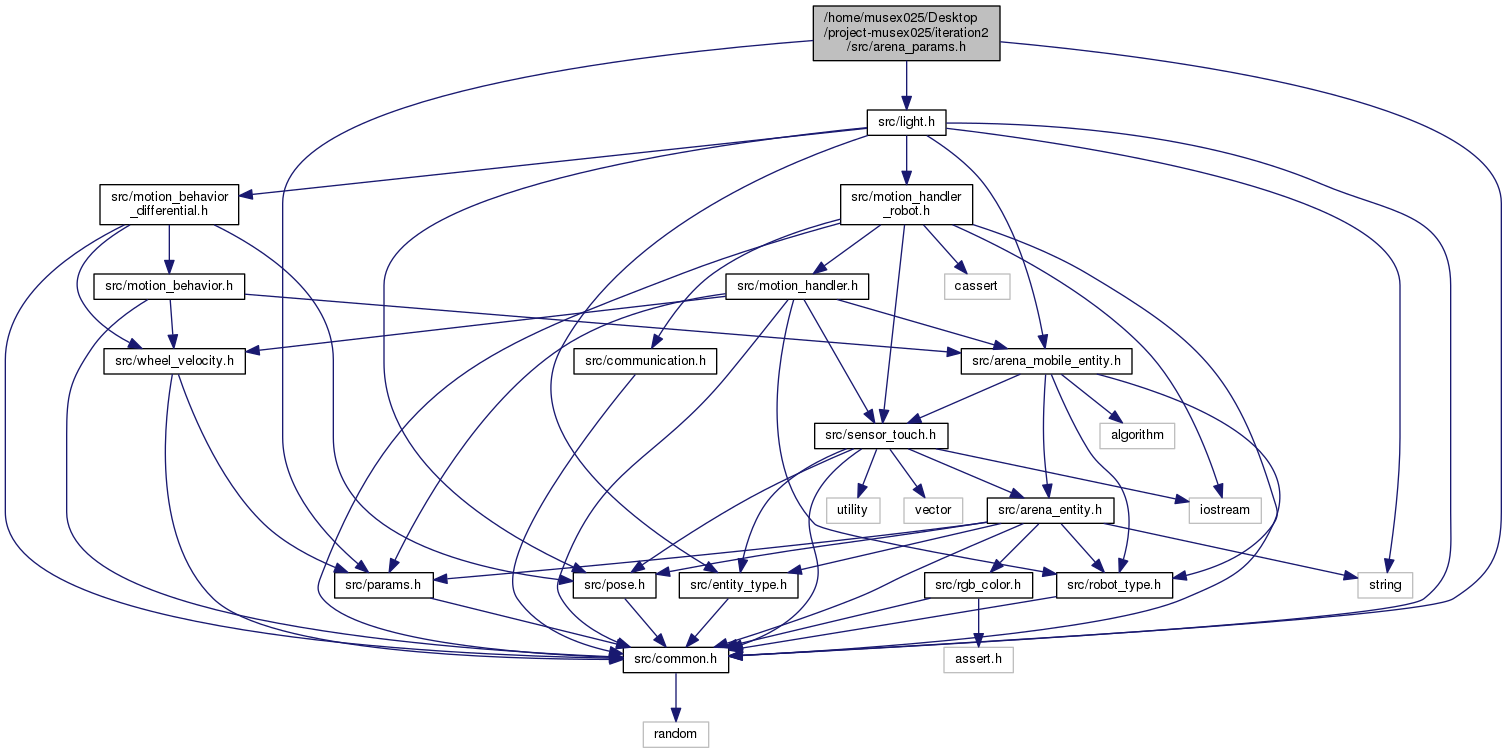
\includegraphics[width=350pt]{arena__params_8h__incl}
\end{center}
\end{figure}
This graph shows which files directly or indirectly include this file\+:\nopagebreak
\begin{figure}[H]
\begin{center}
\leavevmode
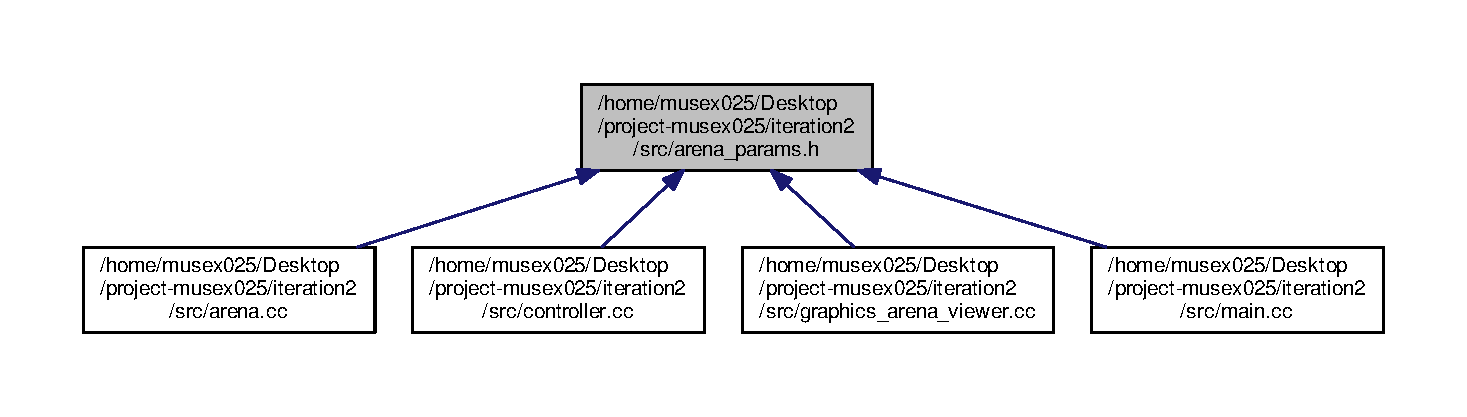
\includegraphics[width=350pt]{arena__params_8h__dep__incl}
\end{center}
\end{figure}
\subsection*{Classes}
\begin{DoxyCompactItemize}
\item 
struct \hyperlink{structarena__params}{arena\+\_\+params}
\begin{DoxyCompactList}\small\item\em Struct holding parameters for initializing the \hyperlink{classArena}{Arena}. \end{DoxyCompactList}\end{DoxyCompactItemize}
\subsection*{Functions}
\begin{DoxyCompactItemize}
\item 
{\bfseries N\+A\+M\+E\+S\+P\+A\+C\+E\+\_\+\+B\+E\+G\+IN} (csci3081)\hypertarget{arena__params_8h_a5eaf22d0e7e2a0f12c6a660a6b011297}{}\label{arena__params_8h_a5eaf22d0e7e2a0f12c6a660a6b011297}

\item 
{\bfseries N\+A\+M\+E\+S\+P\+A\+C\+E\+\_\+\+E\+ND} (csci3081)\hypertarget{arena__params_8h_a0bc8eb973c3aef52acd7429898ace1cd}{}\label{arena__params_8h_a0bc8eb973c3aef52acd7429898ace1cd}

\end{DoxyCompactItemize}


\subsection{Detailed Description}
\begin{DoxyCopyright}{Copyright}
2017 3081 Staff, All rights reserved. 
\end{DoxyCopyright}

\hypertarget{common_8h}{}\section{src/common.h File Reference}
\label{common_8h}\index{src/common.\+h@{src/common.\+h}}
{\ttfamily \#include $<$random$>$}\\*
Include dependency graph for common.\+h\+:\nopagebreak
\begin{figure}[H]
\begin{center}
\leavevmode
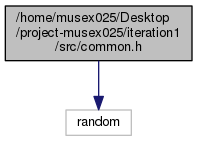
\includegraphics[width=159pt]{common_8h__incl}
\end{center}
\end{figure}
This graph shows which files directly or indirectly include this file\+:\nopagebreak
\begin{figure}[H]
\begin{center}
\leavevmode
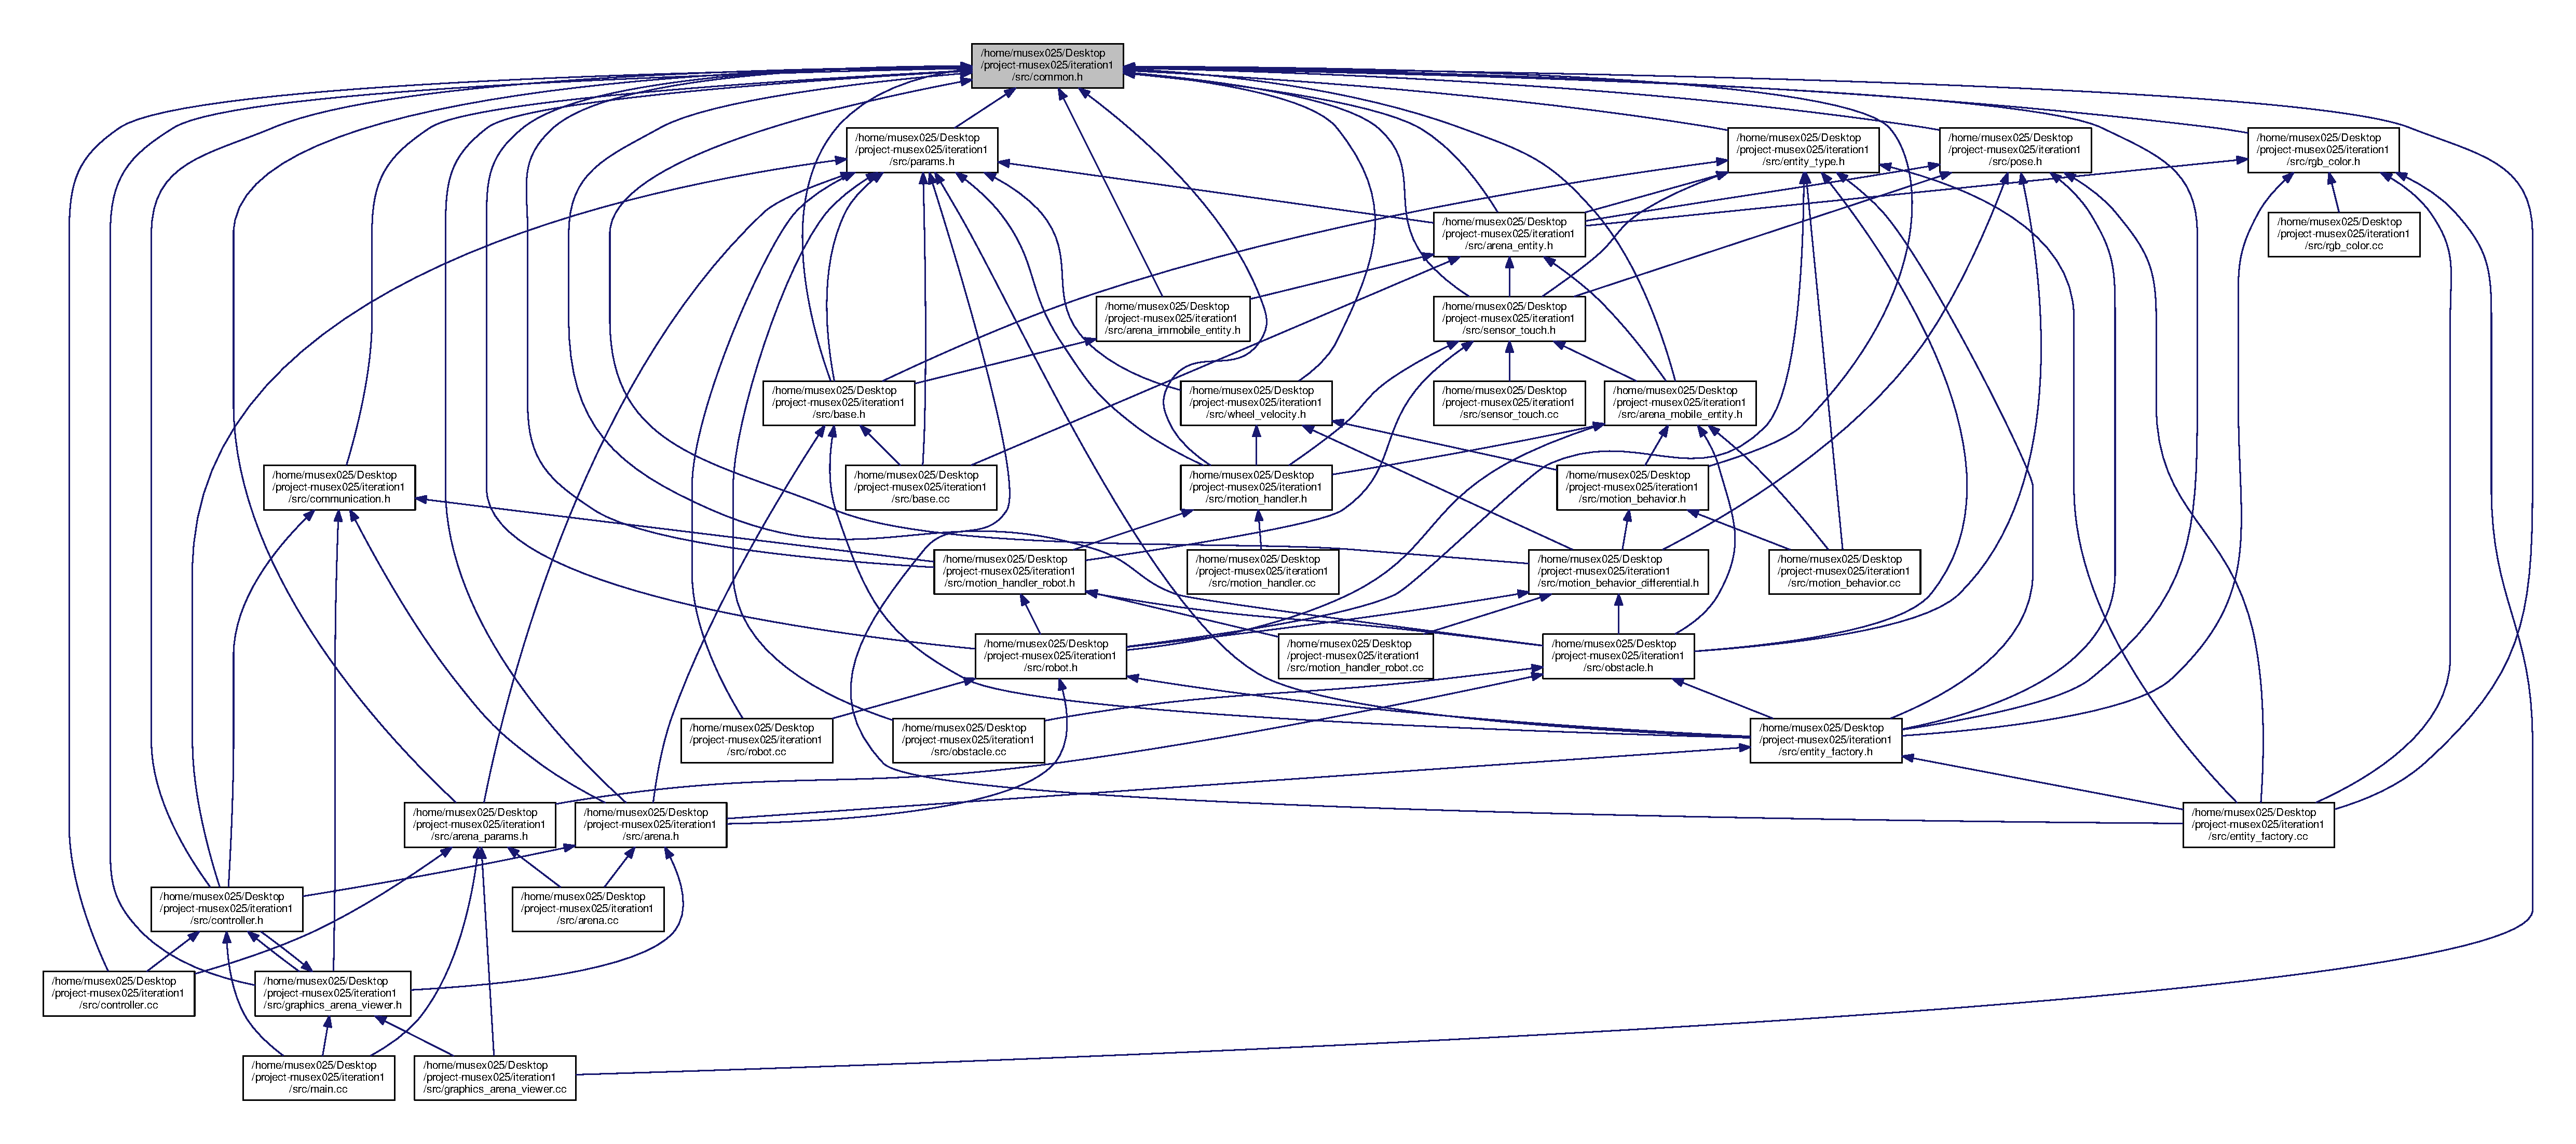
\includegraphics[width=350pt]{common_8h__dep__incl}
\end{center}
\end{figure}
\subsection*{Macros}
\begin{DoxyCompactItemize}
\item 
\#define {\bfseries N\+A\+M\+E\+S\+P\+A\+C\+E\+\_\+\+B\+E\+G\+IN}(name)~namespace name \{\hypertarget{common_8h_a577cd817cb71b655998cad4387cdaeba}{}\label{common_8h_a577cd817cb71b655998cad4387cdaeba}

\item 
\#define {\bfseries N\+A\+M\+E\+S\+P\+A\+C\+E\+\_\+\+E\+ND}(name)~\}\hypertarget{common_8h_a12bb24ea980ca8fb1f46b1992bc9c83a}{}\label{common_8h_a12bb24ea980ca8fb1f46b1992bc9c83a}

\item 
\#define \hyperlink{common_8h_a2e3484535ee610c8e19e9859563abe48}{\+\_\+\+\_\+unused}~\+\_\+\+\_\+attribute\+\_\+\+\_\+((unused))
\end{DoxyCompactItemize}
\subsection*{Functions}
\begin{DoxyCompactItemize}
\item 
{\footnotesize template$<$typename T $>$ }\\T \hyperlink{common_8h_ac14593f15572ef118d7bc7381b372b94}{random\+\_\+num} (T min, T max)
\begin{DoxyCompactList}\small\item\em A template method for random number generation. \end{DoxyCompactList}\end{DoxyCompactItemize}


\subsection{Detailed Description}
\begin{DoxyCopyright}{Copyright}
2017 3081 Staff, All rights reserved. 
\end{DoxyCopyright}


\subsection{Macro Definition Documentation}
\index{common.\+h@{common.\+h}!\+\_\+\+\_\+unused@{\+\_\+\+\_\+unused}}
\index{\+\_\+\+\_\+unused@{\+\_\+\+\_\+unused}!common.\+h@{common.\+h}}
\subsubsection[{\texorpdfstring{\+\_\+\+\_\+unused}{__unused}}]{\setlength{\rightskip}{0pt plus 5cm}\#define \+\_\+\+\_\+unused~\+\_\+\+\_\+attribute\+\_\+\+\_\+((unused))}\hypertarget{common_8h_a2e3484535ee610c8e19e9859563abe48}{}\label{common_8h_a2e3484535ee610c8e19e9859563abe48}
This should be placed in front of any variable defined but not used to satisfy the compiler -\/ otherwise a warning is given. 

\subsection{Function Documentation}
\index{common.\+h@{common.\+h}!random\+\_\+num@{random\+\_\+num}}
\index{random\+\_\+num@{random\+\_\+num}!common.\+h@{common.\+h}}
\subsubsection[{\texorpdfstring{random\+\_\+num(\+T min, T max)}{random_num(T min, T max)}}]{\setlength{\rightskip}{0pt plus 5cm}template$<$typename T $>$ T random\+\_\+num (
\begin{DoxyParamCaption}
\item[{T}]{min, }
\item[{T}]{max}
\end{DoxyParamCaption}
)}\hypertarget{common_8h_ac14593f15572ef118d7bc7381b372b94}{}\label{common_8h_ac14593f15572ef118d7bc7381b372b94}


A template method for random number generation. 


\begin{DoxyTemplParams}{Template Parameters}
{\em T} & The type of the input/return values. Can be any primitive numeric type (e.\+g. {\ttfamily int}). \\
\hline
\end{DoxyTemplParams}

\begin{DoxyParams}{Parameters}
{\em min} & The (inclusive) minimum of the generated value. \\
\hline
{\em max} & The (exclusive) maximum of the generated value.\\
\hline
\end{DoxyParams}
\begin{DoxyReturn}{Returns}
A pseudo-\/randomly generated number in the range of \mbox{[}min, max).
\end{DoxyReturn}
Reference\+: \href{https://stackoverflow.com/a/19728404}{\tt https\+://stackoverflow.\+com/a/19728404} 
\hypertarget{communication_8h}{}\section{src/communication.h File Reference}
\label{communication_8h}\index{src/communication.\+h@{src/communication.\+h}}
{\ttfamily \#include \char`\"{}src/common.\+h\char`\"{}}\\*
Include dependency graph for communication.\+h\+:\nopagebreak
\begin{figure}[H]
\begin{center}
\leavevmode
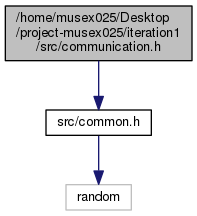
\includegraphics[width=187pt]{communication_8h__incl}
\end{center}
\end{figure}
This graph shows which files directly or indirectly include this file\+:\nopagebreak
\begin{figure}[H]
\begin{center}
\leavevmode
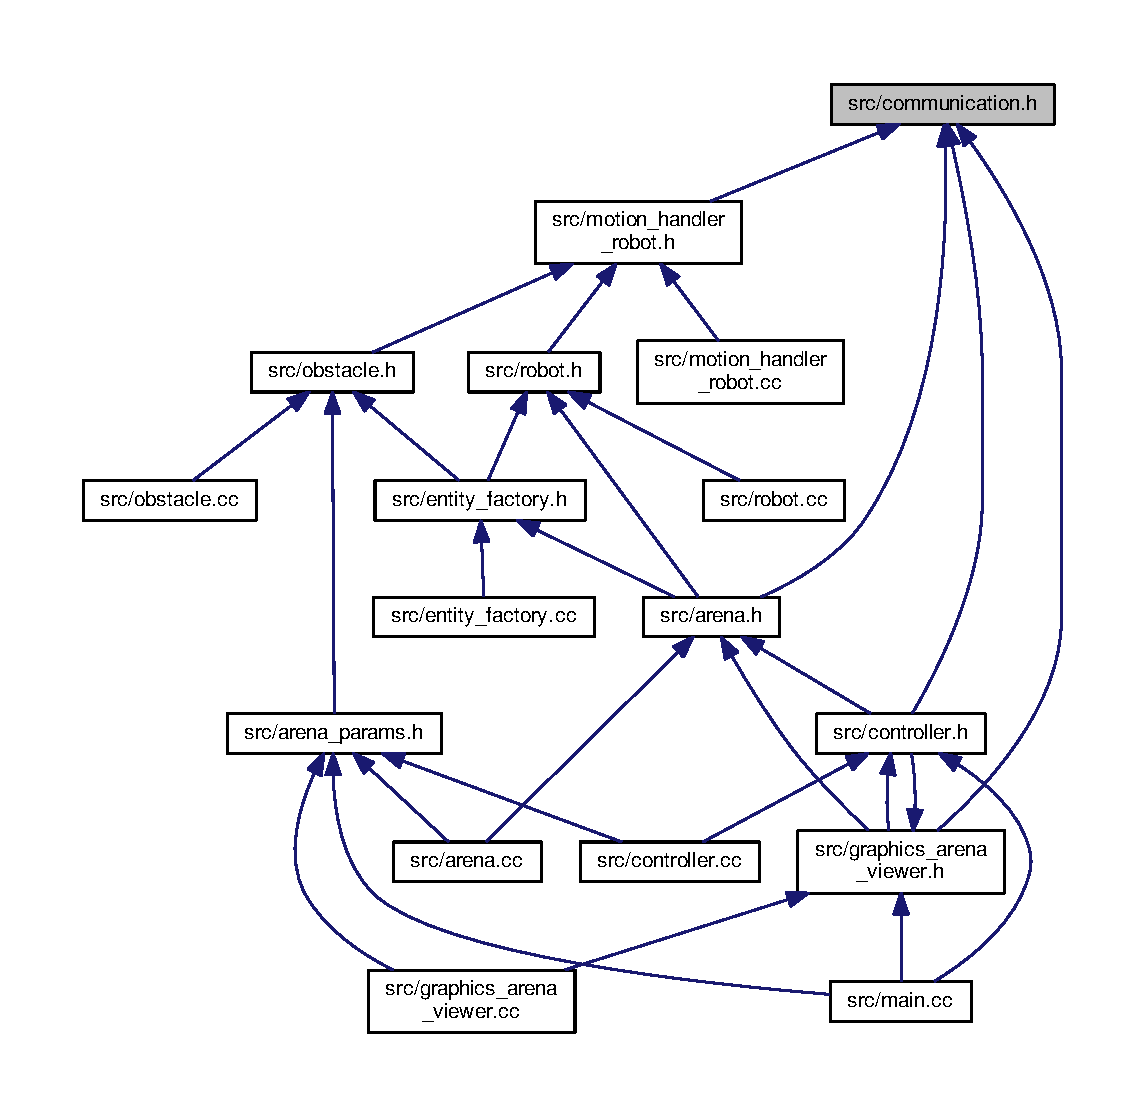
\includegraphics[width=350pt]{communication_8h__dep__incl}
\end{center}
\end{figure}
\subsection*{Enumerations}
\begin{DoxyCompactItemize}
\item 
enum {\bfseries Communication} \{ \\*
{\bfseries k\+Key\+Up}, 
{\bfseries k\+Key\+Down}, 
{\bfseries k\+Key\+Right}, 
{\bfseries k\+Key\+Left}, 
\\*
{\bfseries k\+Play}, 
{\bfseries k\+Pause}, 
{\bfseries k\+New\+Game}, 
{\bfseries k\+Increase\+Speed}, 
\\*
{\bfseries k\+Decrease\+Speed}, 
{\bfseries k\+Turn\+Right}, 
{\bfseries k\+Turn\+Left}, 
{\bfseries k\+Reset}, 
\\*
{\bfseries k\+Won}, 
{\bfseries k\+Lost}, 
{\bfseries k\+None}
 \}\hypertarget{communication_8h_a836c27e2d64d0efa4a526150bdf6f3e5}{}\label{communication_8h_a836c27e2d64d0efa4a526150bdf6f3e5}

\end{DoxyCompactItemize}
\subsection*{Functions}
\begin{DoxyCompactItemize}
\item 
{\bfseries N\+A\+M\+E\+S\+P\+A\+C\+E\+\_\+\+B\+E\+G\+IN} (csci3081)\hypertarget{communication_8h_a5eaf22d0e7e2a0f12c6a660a6b011297}{}\label{communication_8h_a5eaf22d0e7e2a0f12c6a660a6b011297}

\item 
{\bfseries N\+A\+M\+E\+S\+P\+A\+C\+E\+\_\+\+E\+ND} (csci3081)\hypertarget{communication_8h_a0bc8eb973c3aef52acd7429898ace1cd}{}\label{communication_8h_a0bc8eb973c3aef52acd7429898ace1cd}

\end{DoxyCompactItemize}


\subsection{Detailed Description}
\begin{DoxyCopyright}{Copyright}
2017 3081 Staff, All rights reserved. 
\end{DoxyCopyright}

\hypertarget{controller_8cc}{}\section{/home/musex025/\+Desktop/project-\/musex025/iteration2/src/controller.cc File Reference}
\label{controller_8cc}\index{/home/musex025/\+Desktop/project-\/musex025/iteration2/src/controller.\+cc@{/home/musex025/\+Desktop/project-\/musex025/iteration2/src/controller.\+cc}}
{\ttfamily \#include $<$nanogui/nanogui.\+h$>$}\\*
{\ttfamily \#include $<$string$>$}\\*
{\ttfamily \#include \char`\"{}src/arena\+\_\+params.\+h\char`\"{}}\\*
{\ttfamily \#include \char`\"{}src/common.\+h\char`\"{}}\\*
{\ttfamily \#include \char`\"{}src/controller.\+h\char`\"{}}\\*
Include dependency graph for controller.\+cc\+:\nopagebreak
\begin{figure}[H]
\begin{center}
\leavevmode
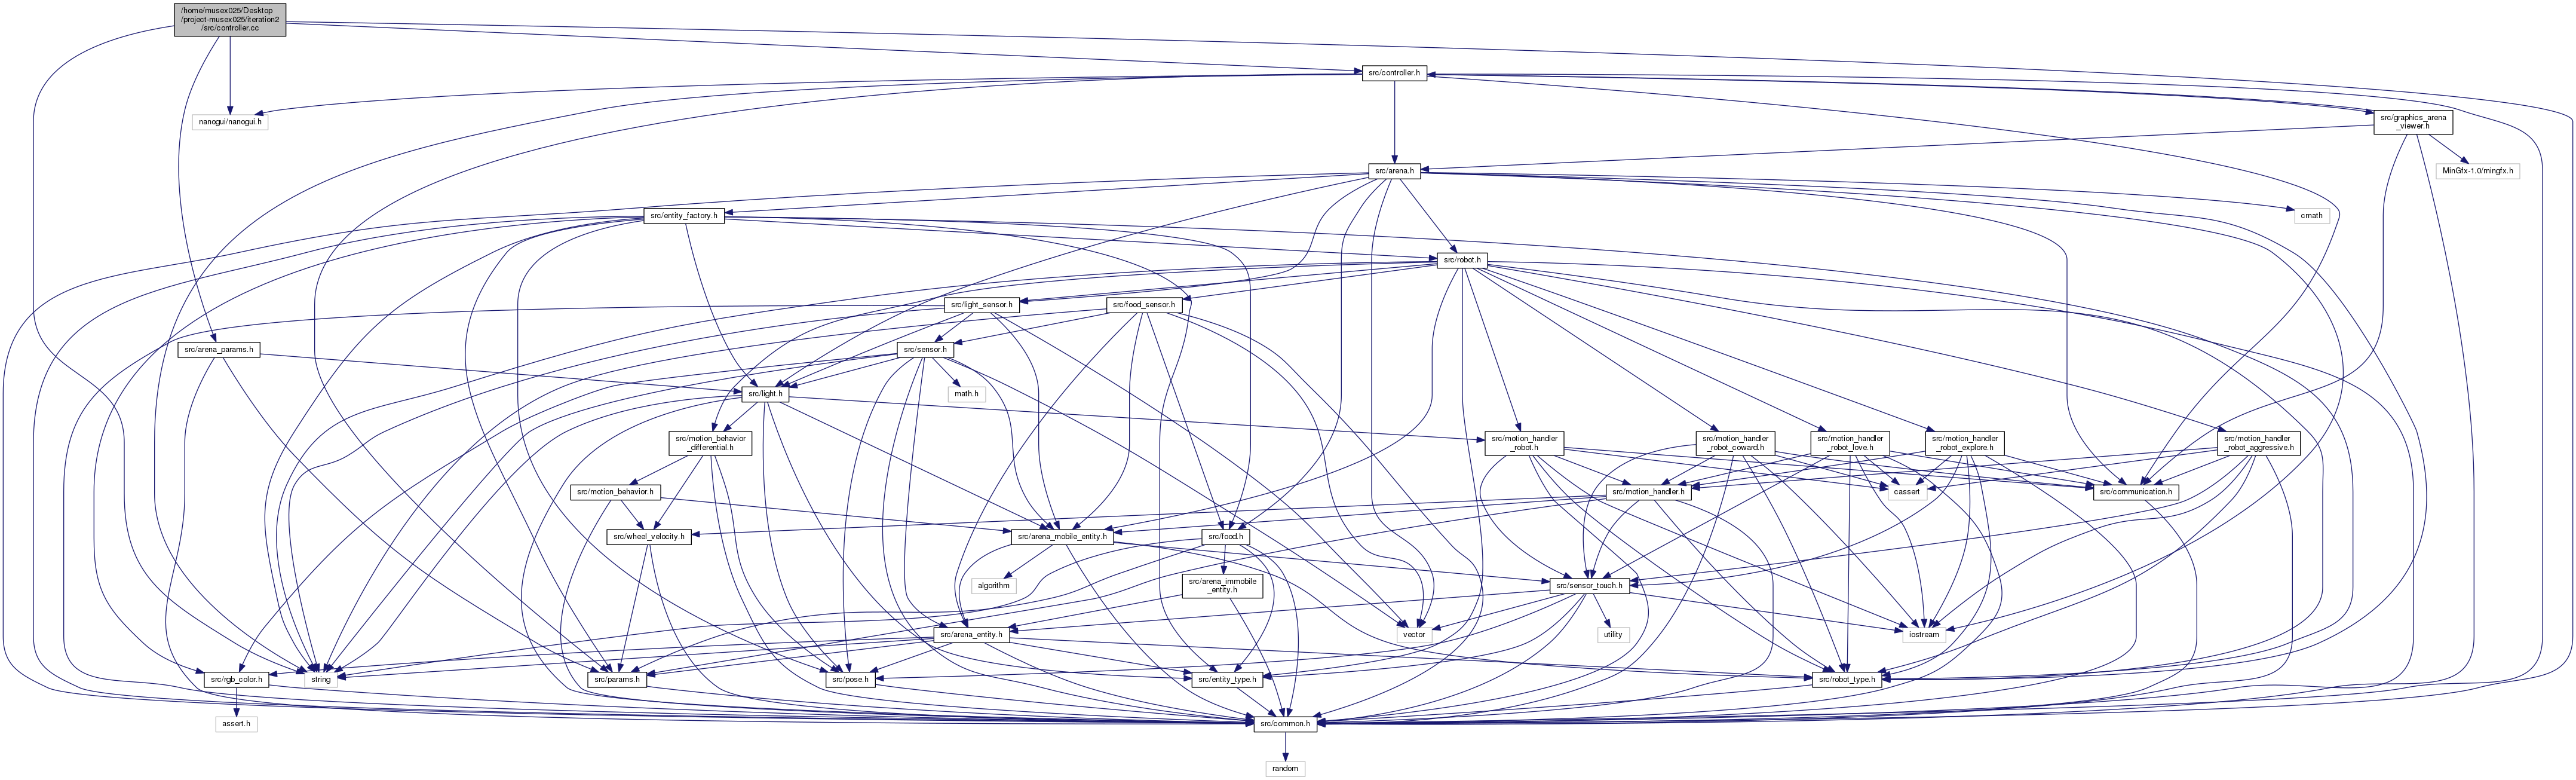
\includegraphics[width=350pt]{controller_8cc__incl}
\end{center}
\end{figure}
\subsection*{Functions}
\begin{DoxyCompactItemize}
\item 
{\bfseries N\+A\+M\+E\+S\+P\+A\+C\+E\+\_\+\+B\+E\+G\+IN} (csci3081)\hypertarget{controller_8cc_a5eaf22d0e7e2a0f12c6a660a6b011297}{}\label{controller_8cc_a5eaf22d0e7e2a0f12c6a660a6b011297}

\item 
{\bfseries N\+A\+M\+E\+S\+P\+A\+C\+E\+\_\+\+E\+ND} (csci3081)\hypertarget{controller_8cc_a0bc8eb973c3aef52acd7429898ace1cd}{}\label{controller_8cc_a0bc8eb973c3aef52acd7429898ace1cd}

\end{DoxyCompactItemize}


\subsection{Detailed Description}
\begin{DoxyCopyright}{Copyright}
2017 3081 Staff, All rights reserved. 
\end{DoxyCopyright}

\hypertarget{controller_8h}{}\section{src/controller.h File Reference}
\label{controller_8h}\index{src/controller.\+h@{src/controller.\+h}}
{\ttfamily \#include $<$nanogui/nanogui.\+h$>$}\newline
{\ttfamily \#include $<$string$>$}\newline
{\ttfamily \#include \char`\"{}src/arena.\+h\char`\"{}}\newline
{\ttfamily \#include \char`\"{}src/common.\+h\char`\"{}}\newline
{\ttfamily \#include \char`\"{}src/communication.\+h\char`\"{}}\newline
{\ttfamily \#include \char`\"{}src/graphics\+\_\+arena\+\_\+viewer.\+h\char`\"{}}\newline
{\ttfamily \#include \char`\"{}src/params.\+h\char`\"{}}\newline
\subsection*{Classes}
\begin{DoxyCompactItemize}
\item 
class \mbox{\hyperlink{class_controller}{Controller}}
\begin{DoxyCompactList}\small\item\em \mbox{\hyperlink{class_controller}{Controller}} that mediates \mbox{\hyperlink{class_arena}{Arena}} and \mbox{\hyperlink{class_graphics_arena_viewer}{Graphics\+Arena\+Viewer}} communication. \end{DoxyCompactList}\end{DoxyCompactItemize}
\subsection*{Functions}
\begin{DoxyCompactItemize}
\item 
\mbox{\Hypertarget{controller_8h_a5eaf22d0e7e2a0f12c6a660a6b011297}\label{controller_8h_a5eaf22d0e7e2a0f12c6a660a6b011297}} 
{\bfseries N\+A\+M\+E\+S\+P\+A\+C\+E\+\_\+\+B\+E\+G\+IN} (csci3081)
\item 
\mbox{\Hypertarget{controller_8h_a0bc8eb973c3aef52acd7429898ace1cd}\label{controller_8h_a0bc8eb973c3aef52acd7429898ace1cd}} 
{\bfseries N\+A\+M\+E\+S\+P\+A\+C\+E\+\_\+\+E\+ND} (csci3081)
\end{DoxyCompactItemize}


\subsection{Detailed Description}
\begin{DoxyCopyright}{Copyright}
2017 3081 Staff, All rights reserved. 
\end{DoxyCopyright}

\hypertarget{entity__factory_8cc}{}\section{/home/musex025/\+Desktop/project-\/musex025/iteration1/src/entity\+\_\+factory.cc File Reference}
\label{entity__factory_8cc}\index{/home/musex025/\+Desktop/project-\/musex025/iteration1/src/entity\+\_\+factory.\+cc@{/home/musex025/\+Desktop/project-\/musex025/iteration1/src/entity\+\_\+factory.\+cc}}
{\ttfamily \#include $<$string$>$}\\*
{\ttfamily \#include $<$ctime$>$}\\*
{\ttfamily \#include $<$iostream$>$}\\*
{\ttfamily \#include \char`\"{}src/common.\+h\char`\"{}}\\*
{\ttfamily \#include \char`\"{}src/entity\+\_\+factory.\+h\char`\"{}}\\*
{\ttfamily \#include \char`\"{}src/entity\+\_\+type.\+h\char`\"{}}\\*
{\ttfamily \#include \char`\"{}src/params.\+h\char`\"{}}\\*
{\ttfamily \#include \char`\"{}src/pose.\+h\char`\"{}}\\*
{\ttfamily \#include \char`\"{}src/rgb\+\_\+color.\+h\char`\"{}}\\*
Include dependency graph for entity\+\_\+factory.\+cc\+:
\nopagebreak
\begin{figure}[H]
\begin{center}
\leavevmode
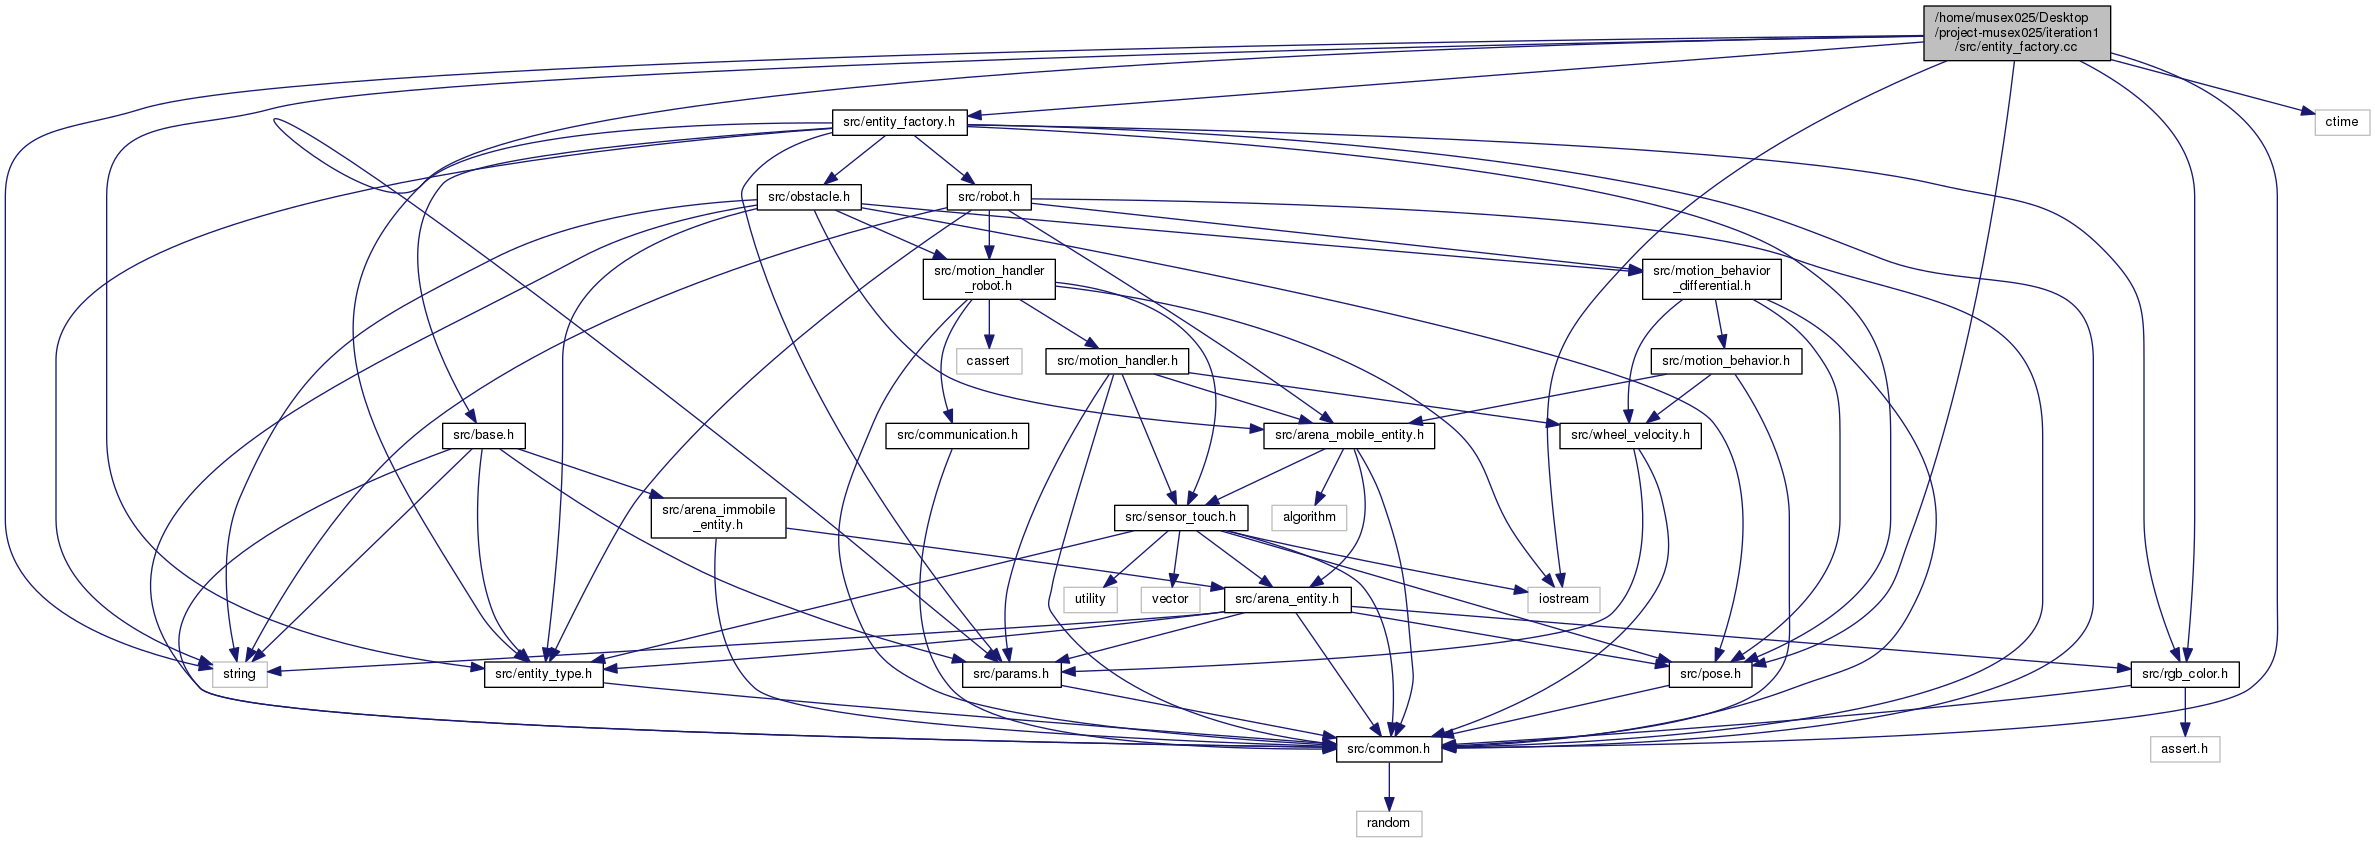
\includegraphics[width=350pt]{entity__factory_8cc__incl}
\end{center}
\end{figure}
\subsection*{Functions}
\begin{DoxyCompactItemize}
\item 
{\bfseries N\+A\+M\+E\+S\+P\+A\+C\+E\+\_\+\+B\+E\+G\+IN} (csci3081)\hypertarget{entity__factory_8cc_a5eaf22d0e7e2a0f12c6a660a6b011297}{}\label{entity__factory_8cc_a5eaf22d0e7e2a0f12c6a660a6b011297}

\item 
{\bfseries N\+A\+M\+E\+S\+P\+A\+C\+E\+\_\+\+E\+ND} (csci3081)\hypertarget{entity__factory_8cc_a0bc8eb973c3aef52acd7429898ace1cd}{}\label{entity__factory_8cc_a0bc8eb973c3aef52acd7429898ace1cd}

\end{DoxyCompactItemize}


\subsection{Detailed Description}
\begin{DoxyCopyright}{Copyright}
2017 3081 Staff, All rights reserved. 
\end{DoxyCopyright}

\hypertarget{entity__factory_8h}{}\section{/home/musex025/\+Desktop/project-\/musex025/iteration1/src/entity\+\_\+factory.h File Reference}
\label{entity__factory_8h}\index{/home/musex025/\+Desktop/project-\/musex025/iteration1/src/entity\+\_\+factory.\+h@{/home/musex025/\+Desktop/project-\/musex025/iteration1/src/entity\+\_\+factory.\+h}}
{\ttfamily \#include $<$string$>$}\\*
{\ttfamily \#include \char`\"{}src/base.\+h\char`\"{}}\\*
{\ttfamily \#include \char`\"{}src/common.\+h\char`\"{}}\\*
{\ttfamily \#include \char`\"{}src/entity\+\_\+type.\+h\char`\"{}}\\*
{\ttfamily \#include \char`\"{}src/obstacle.\+h\char`\"{}}\\*
{\ttfamily \#include \char`\"{}src/params.\+h\char`\"{}}\\*
{\ttfamily \#include \char`\"{}src/pose.\+h\char`\"{}}\\*
{\ttfamily \#include \char`\"{}src/rgb\+\_\+color.\+h\char`\"{}}\\*
{\ttfamily \#include \char`\"{}src/robot.\+h\char`\"{}}\\*
Include dependency graph for entity\+\_\+factory.\+h\+:
\nopagebreak
\begin{figure}[H]
\begin{center}
\leavevmode
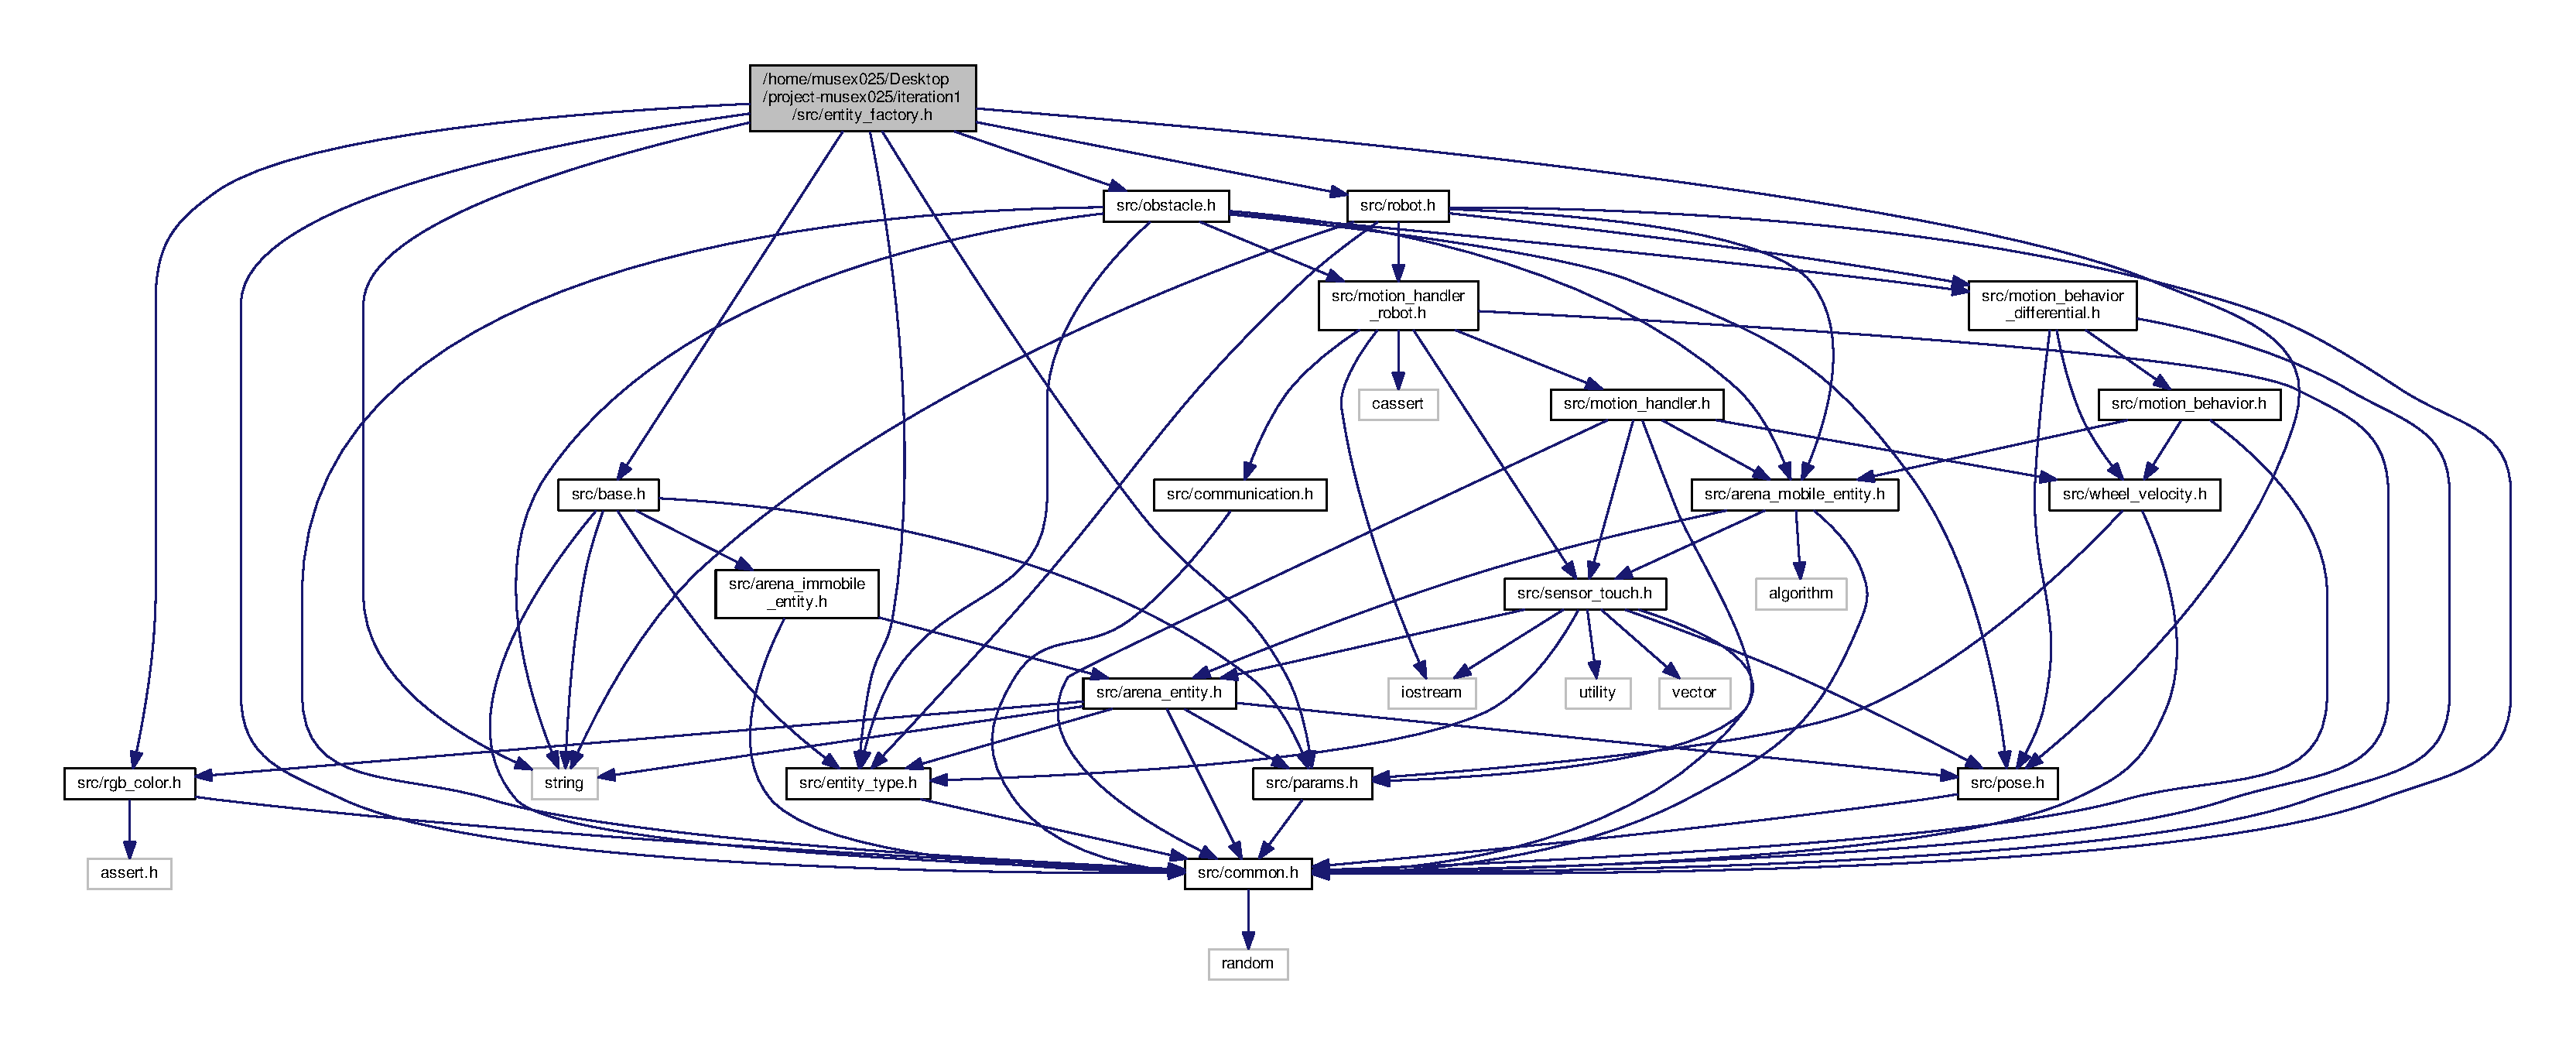
\includegraphics[width=350pt]{entity__factory_8h__incl}
\end{center}
\end{figure}
This graph shows which files directly or indirectly include this file\+:
\nopagebreak
\begin{figure}[H]
\begin{center}
\leavevmode
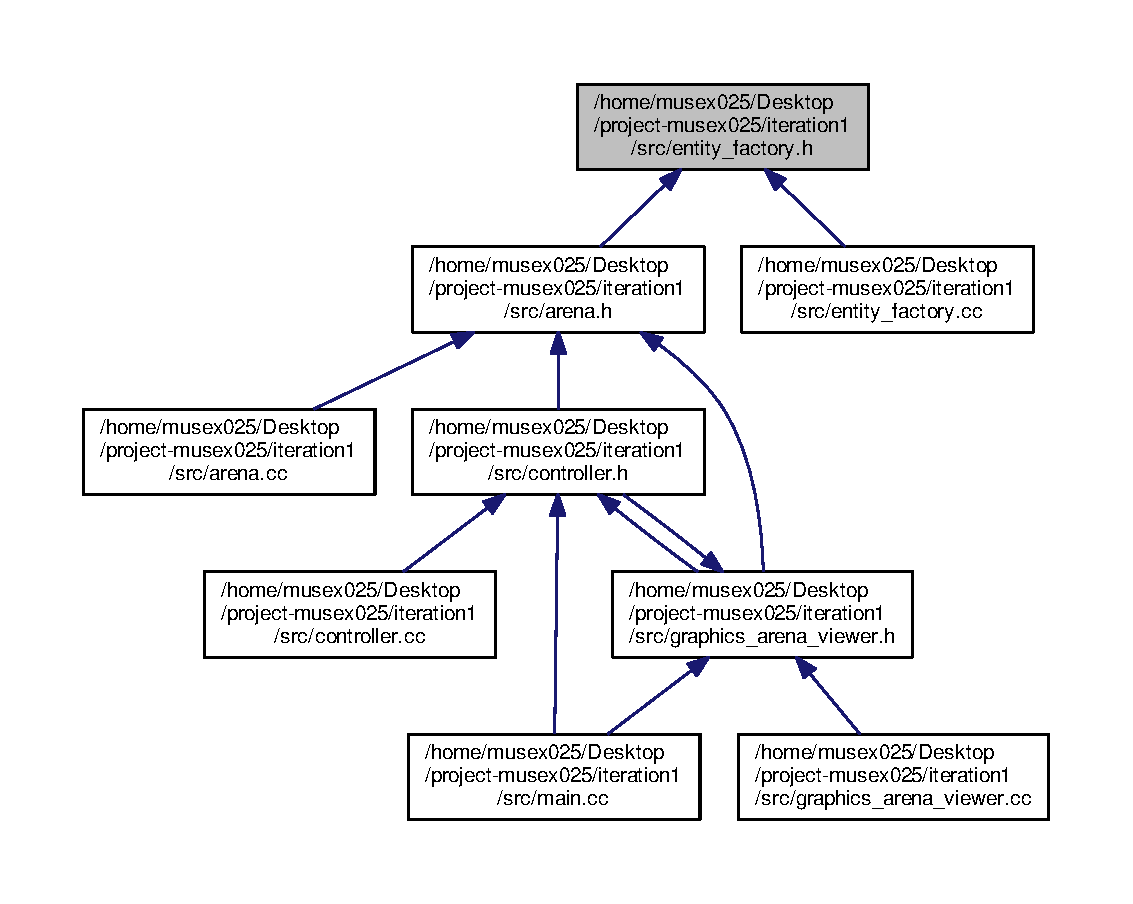
\includegraphics[width=350pt]{entity__factory_8h__dep__incl}
\end{center}
\end{figure}
\subsection*{Classes}
\begin{DoxyCompactItemize}
\item 
class \hyperlink{classEntityFactory}{Entity\+Factory}
\begin{DoxyCompactList}\small\item\em A factory for the instantiation of all types of arena entities. \end{DoxyCompactList}\end{DoxyCompactItemize}
\subsection*{Functions}
\begin{DoxyCompactItemize}
\item 
{\bfseries N\+A\+M\+E\+S\+P\+A\+C\+E\+\_\+\+B\+E\+G\+IN} (csci3081)\hypertarget{entity__factory_8h_a5eaf22d0e7e2a0f12c6a660a6b011297}{}\label{entity__factory_8h_a5eaf22d0e7e2a0f12c6a660a6b011297}

\item 
{\bfseries N\+A\+M\+E\+S\+P\+A\+C\+E\+\_\+\+E\+ND} (csci3081)\hypertarget{entity__factory_8h_a0bc8eb973c3aef52acd7429898ace1cd}{}\label{entity__factory_8h_a0bc8eb973c3aef52acd7429898ace1cd}

\end{DoxyCompactItemize}


\subsection{Detailed Description}
\begin{DoxyCopyright}{Copyright}
2017 3081 Staff, All rights reserved. 
\end{DoxyCopyright}

\hypertarget{entity__type_8h}{}\section{/home/musex025/\+Desktop/project-\/musex025/iteration1/src/entity\+\_\+type.h File Reference}
\label{entity__type_8h}\index{/home/musex025/\+Desktop/project-\/musex025/iteration1/src/entity\+\_\+type.\+h@{/home/musex025/\+Desktop/project-\/musex025/iteration1/src/entity\+\_\+type.\+h}}
{\ttfamily \#include \char`\"{}src/common.\+h\char`\"{}}\\*
Include dependency graph for entity\+\_\+type.\+h\+:
\nopagebreak
\begin{figure}[H]
\begin{center}
\leavevmode
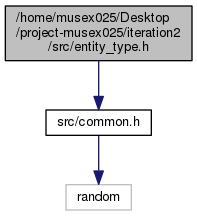
\includegraphics[width=220pt]{entity__type_8h__incl}
\end{center}
\end{figure}
This graph shows which files directly or indirectly include this file\+:
\nopagebreak
\begin{figure}[H]
\begin{center}
\leavevmode
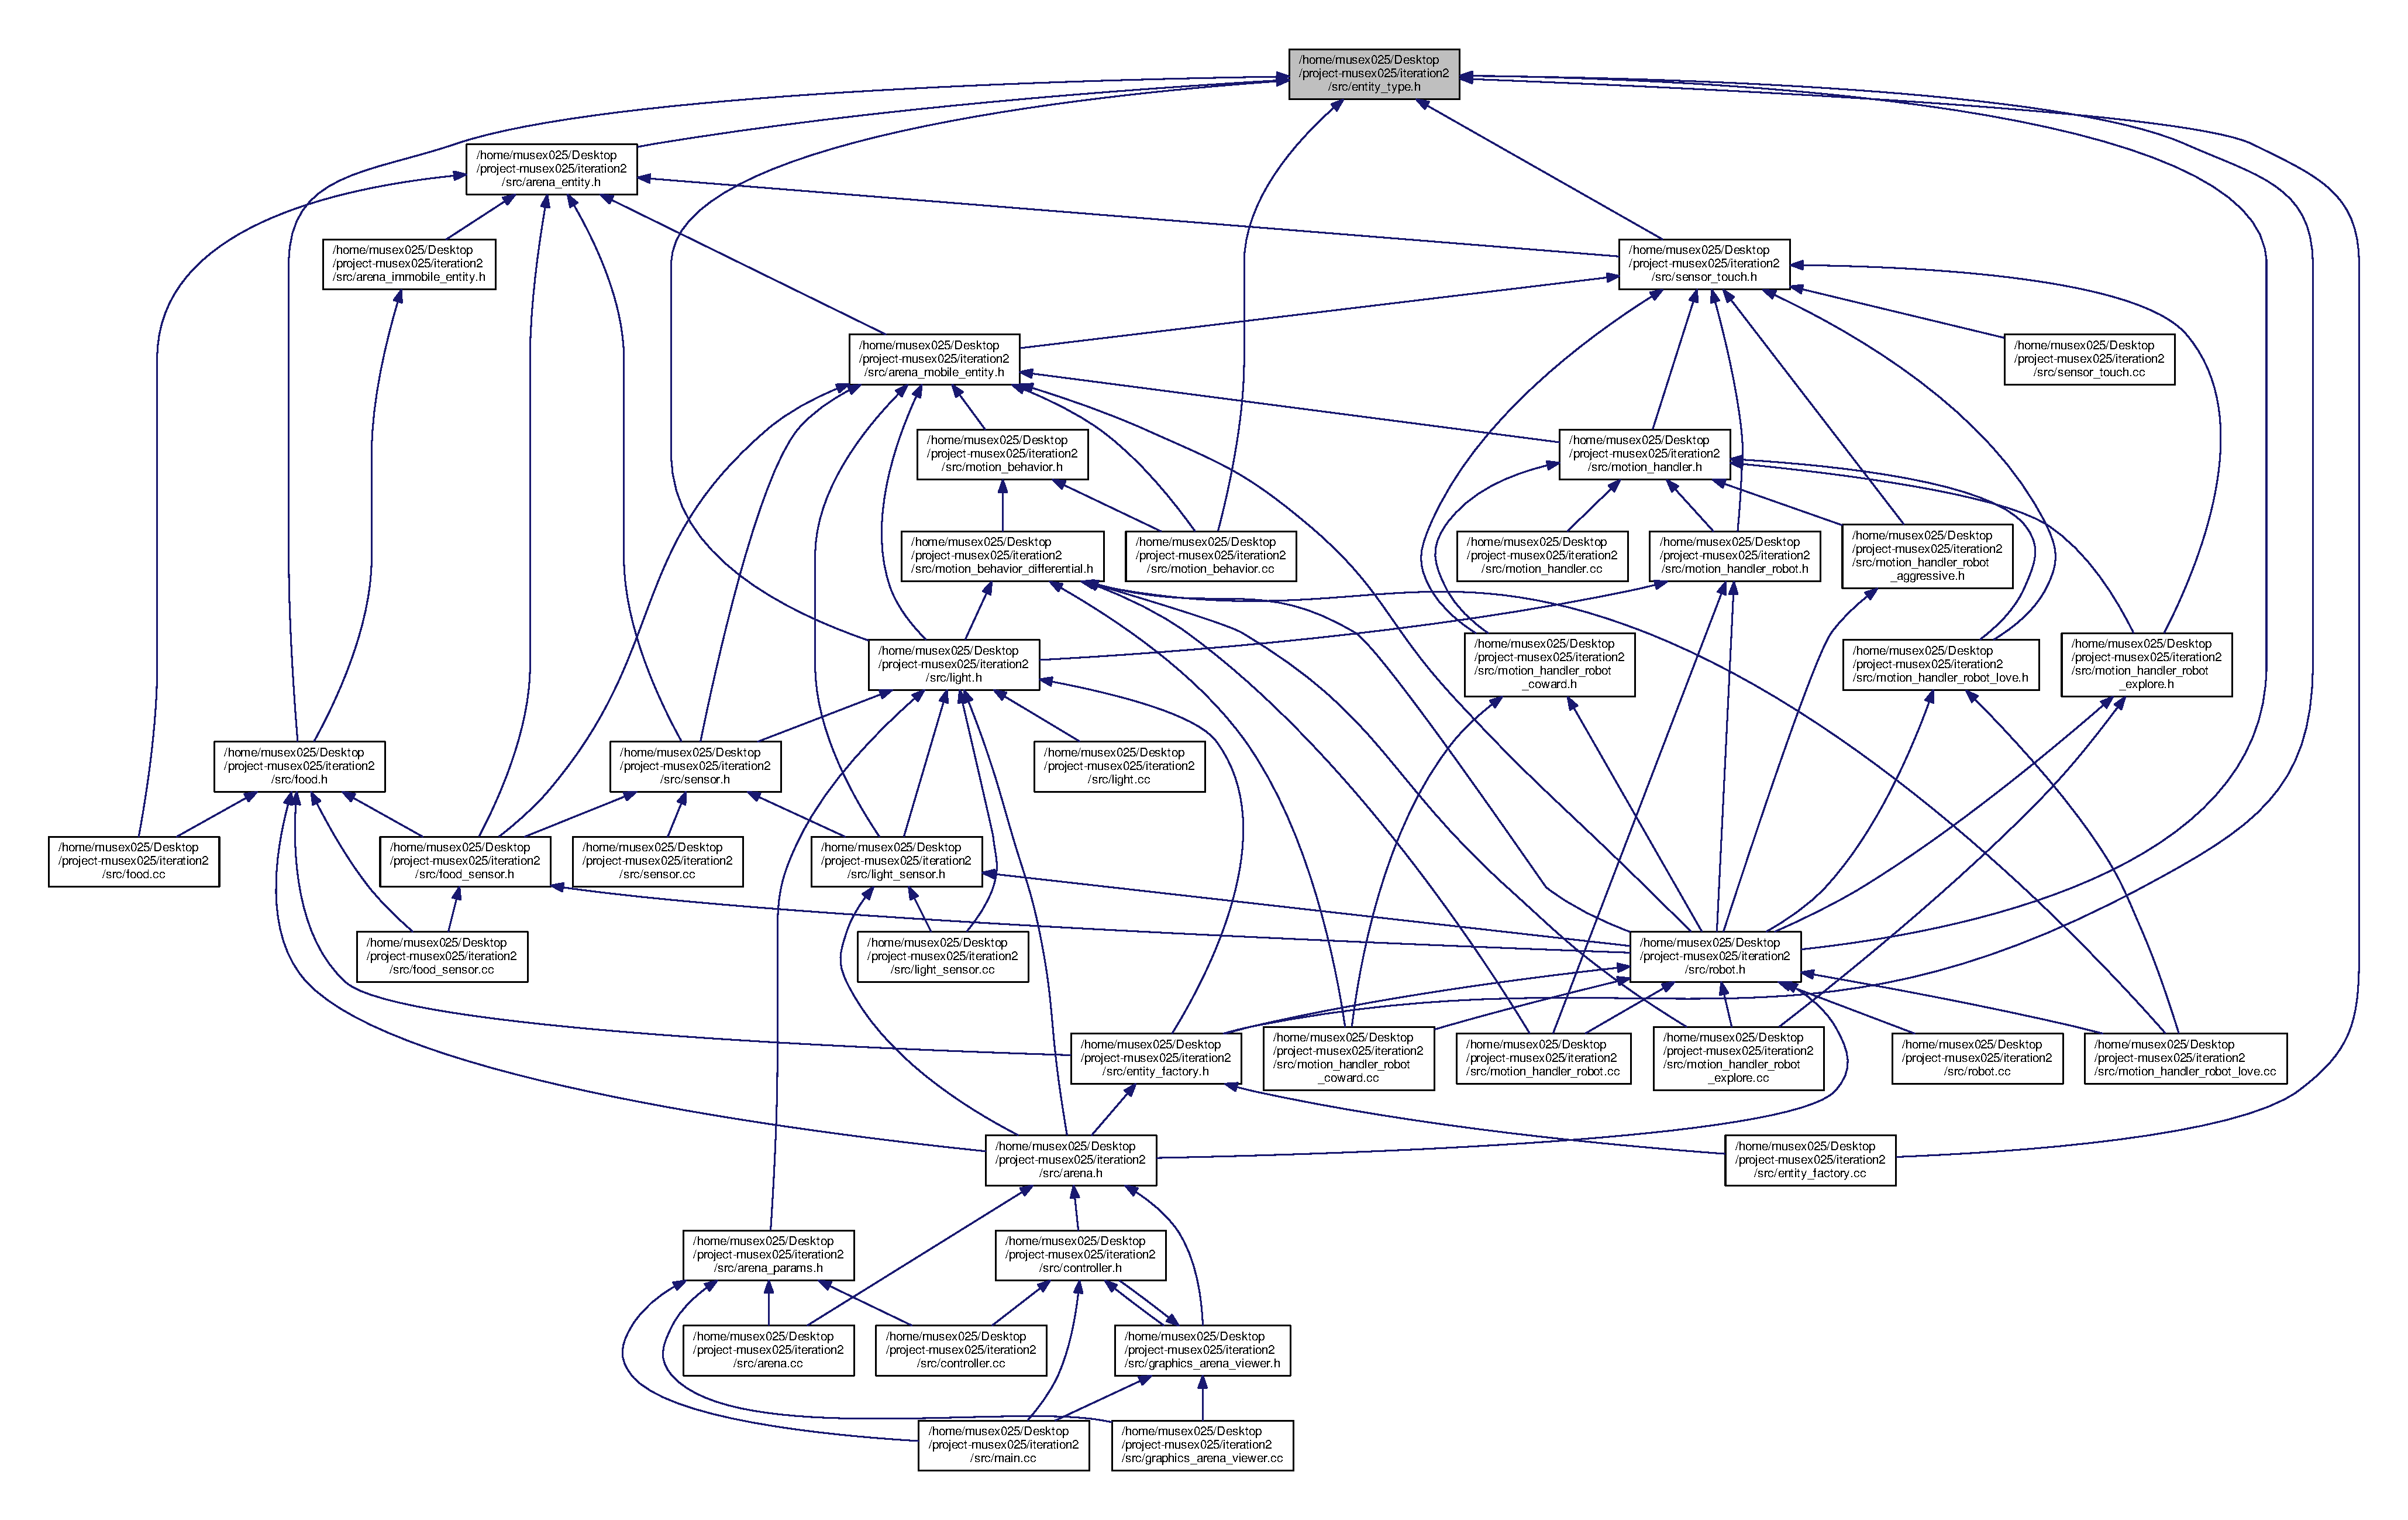
\includegraphics[width=350pt]{entity__type_8h__dep__incl}
\end{center}
\end{figure}
\subsection*{Enumerations}
\begin{DoxyCompactItemize}
\item 
enum {\bfseries Entity\+Type} \{ \\*
{\bfseries k\+Robot}, 
{\bfseries k\+Obstacle}, 
{\bfseries k\+Base}, 
{\bfseries k\+Entity}, 
\\*
{\bfseries k\+Right\+Wall}, 
{\bfseries k\+Left\+Wall}, 
{\bfseries k\+Top\+Wall}, 
{\bfseries k\+Bottom\+Wall}, 
\\*
{\bfseries k\+Undefined}
 \}\hypertarget{entity__type_8h_ad79a57ed3105eb60d991a1aeb4a9dc44}{}\label{entity__type_8h_ad79a57ed3105eb60d991a1aeb4a9dc44}

\end{DoxyCompactItemize}
\subsection*{Functions}
\begin{DoxyCompactItemize}
\item 
{\bfseries N\+A\+M\+E\+S\+P\+A\+C\+E\+\_\+\+B\+E\+G\+IN} (csci3081)\hypertarget{entity__type_8h_a5eaf22d0e7e2a0f12c6a660a6b011297}{}\label{entity__type_8h_a5eaf22d0e7e2a0f12c6a660a6b011297}

\item 
{\bfseries N\+A\+M\+E\+S\+P\+A\+C\+E\+\_\+\+E\+ND} (csci3081)\hypertarget{entity__type_8h_a0bc8eb973c3aef52acd7429898ace1cd}{}\label{entity__type_8h_a0bc8eb973c3aef52acd7429898ace1cd}

\end{DoxyCompactItemize}


\subsection{Detailed Description}
\begin{DoxyCopyright}{Copyright}
2017 3081 Staff, All rights reserved. 
\end{DoxyCopyright}

\hypertarget{food_8cc}{}\section{src/food.cc File Reference}
\label{food_8cc}\index{src/food.\+cc@{src/food.\+cc}}
{\ttfamily \#include \char`\"{}src/food.\+h\char`\"{}}\\*
{\ttfamily \#include \char`\"{}src/params.\+h\char`\"{}}\\*
{\ttfamily \#include \char`\"{}src/arena\+\_\+entity.\+h\char`\"{}}\\*
\subsection*{Functions}
\begin{DoxyCompactItemize}
\item 
{\bfseries N\+A\+M\+E\+S\+P\+A\+C\+E\+\_\+\+B\+E\+G\+IN} (csci3081)\hypertarget{food_8cc_a5eaf22d0e7e2a0f12c6a660a6b011297}{}\label{food_8cc_a5eaf22d0e7e2a0f12c6a660a6b011297}

\item 
{\bfseries N\+A\+M\+E\+S\+P\+A\+C\+E\+\_\+\+E\+ND} (csci3081)\hypertarget{food_8cc_a0bc8eb973c3aef52acd7429898ace1cd}{}\label{food_8cc_a0bc8eb973c3aef52acd7429898ace1cd}

\end{DoxyCompactItemize}


\subsection{Detailed Description}
\begin{DoxyCopyright}{Copyright}
2017 3081 Staff, All rights reserved. 
\end{DoxyCopyright}

\hypertarget{food_8h}{}\section{/home/musex025/\+Desktop/project-\/musex025/iteration2/src/food.h File Reference}
\label{food_8h}\index{/home/musex025/\+Desktop/project-\/musex025/iteration2/src/food.\+h@{/home/musex025/\+Desktop/project-\/musex025/iteration2/src/food.\+h}}
{\ttfamily \#include $<$string$>$}\\*
{\ttfamily \#include \char`\"{}src/params.\+h\char`\"{}}\\*
{\ttfamily \#include \char`\"{}src/arena\+\_\+immobile\+\_\+entity.\+h\char`\"{}}\\*
{\ttfamily \#include \char`\"{}src/common.\+h\char`\"{}}\\*
{\ttfamily \#include \char`\"{}src/entity\+\_\+type.\+h\char`\"{}}\\*
Include dependency graph for food.\+h\+:\nopagebreak
\begin{figure}[H]
\begin{center}
\leavevmode
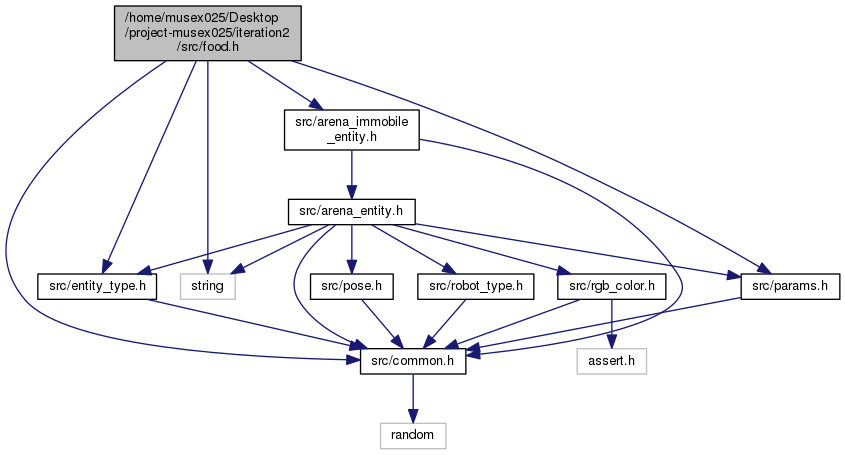
\includegraphics[width=350pt]{food_8h__incl}
\end{center}
\end{figure}
This graph shows which files directly or indirectly include this file\+:\nopagebreak
\begin{figure}[H]
\begin{center}
\leavevmode
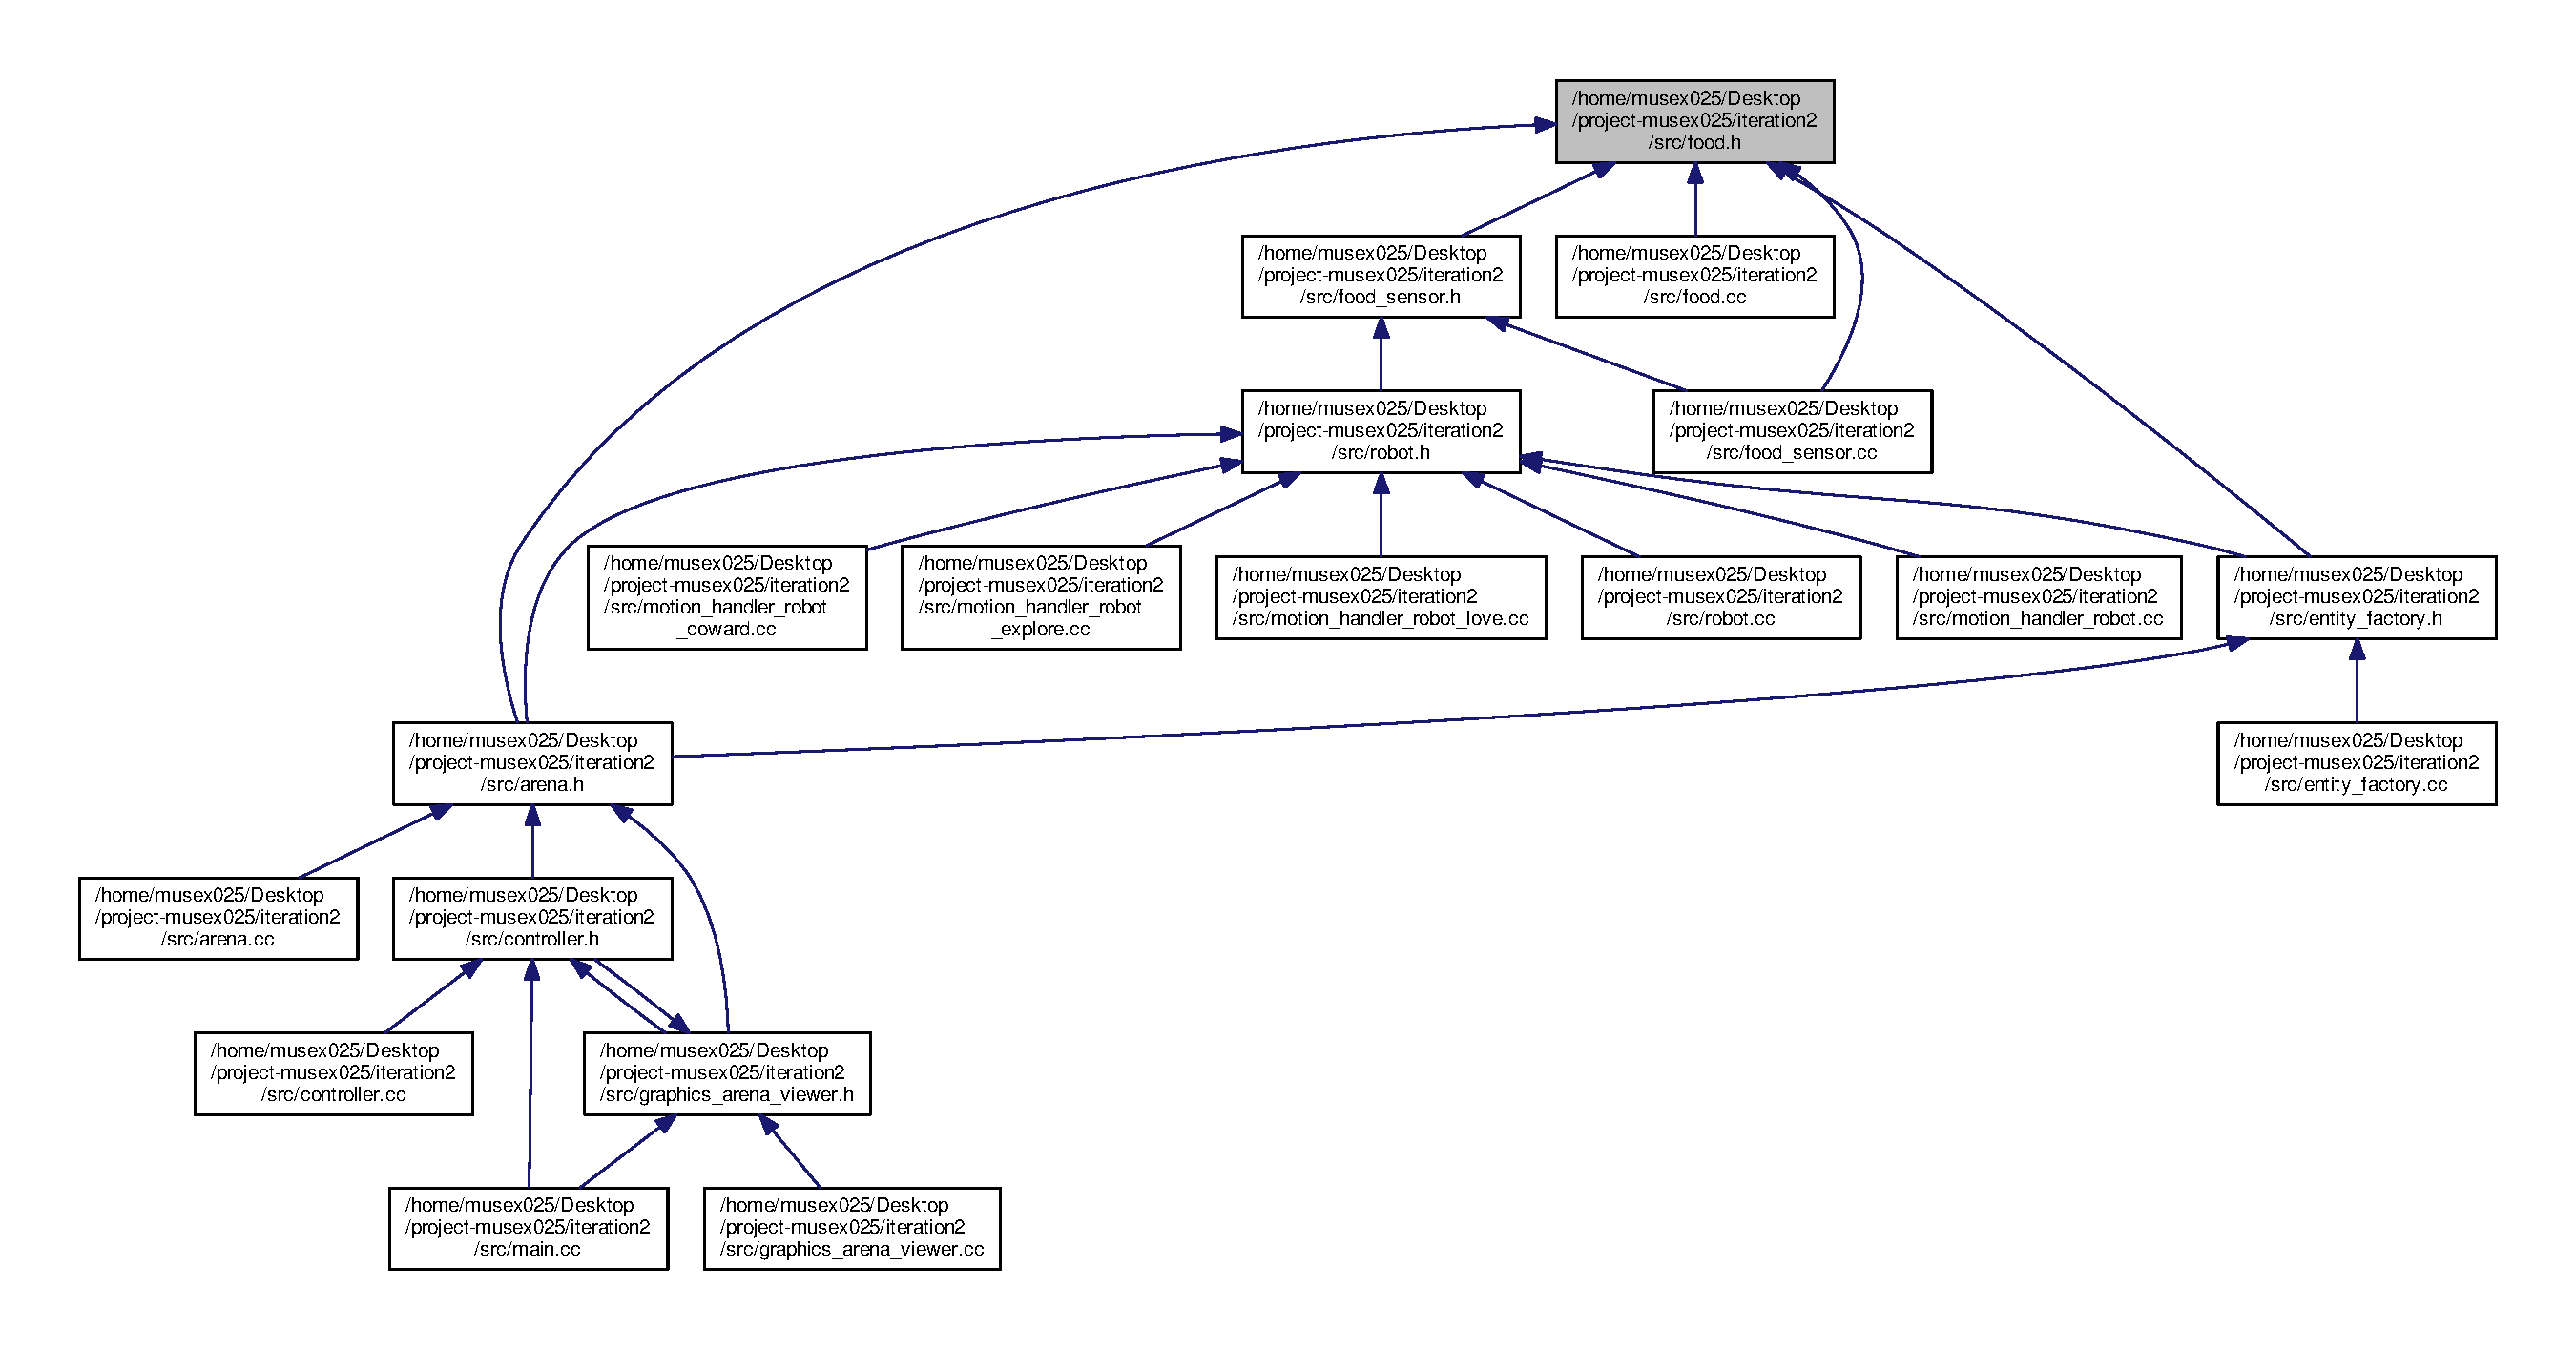
\includegraphics[width=350pt]{food_8h__dep__incl}
\end{center}
\end{figure}
\subsection*{Classes}
\begin{DoxyCompactItemize}
\item 
class \hyperlink{classFood}{Food}
\begin{DoxyCompactList}\small\item\em Class representing a immobile \hyperlink{classFood}{Food} within the \hyperlink{classArena}{Arena}. \end{DoxyCompactList}\end{DoxyCompactItemize}
\subsection*{Functions}
\begin{DoxyCompactItemize}
\item 
{\bfseries N\+A\+M\+E\+S\+P\+A\+C\+E\+\_\+\+B\+E\+G\+IN} (csci3081)\hypertarget{food_8h_a5eaf22d0e7e2a0f12c6a660a6b011297}{}\label{food_8h_a5eaf22d0e7e2a0f12c6a660a6b011297}

\item 
{\bfseries N\+A\+M\+E\+S\+P\+A\+C\+E\+\_\+\+E\+ND} (csci3081)\hypertarget{food_8h_a0bc8eb973c3aef52acd7429898ace1cd}{}\label{food_8h_a0bc8eb973c3aef52acd7429898ace1cd}

\end{DoxyCompactItemize}


\subsection{Detailed Description}
\begin{DoxyCopyright}{Copyright}
2017 3081 Staff, All rights reserved. 
\end{DoxyCopyright}

\hypertarget{food__sensor_8cc}{}\section{src/food\+\_\+sensor.cc File Reference}
\label{food__sensor_8cc}\index{src/food\+\_\+sensor.\+cc@{src/food\+\_\+sensor.\+cc}}
{\ttfamily \#include $<$math.\+h$>$}\newline
{\ttfamily \#include $<$vector$>$}\newline
{\ttfamily \#include \char`\"{}src/food\+\_\+sensor.\+h\char`\"{}}\newline
{\ttfamily \#include \char`\"{}src/food.\+h\char`\"{}}\newline
{\ttfamily \#include \char`\"{}src/params.\+h\char`\"{}}\newline
\subsection*{Functions}
\begin{DoxyCompactItemize}
\item 
\mbox{\Hypertarget{food__sensor_8cc_a5eaf22d0e7e2a0f12c6a660a6b011297}\label{food__sensor_8cc_a5eaf22d0e7e2a0f12c6a660a6b011297}} 
{\bfseries N\+A\+M\+E\+S\+P\+A\+C\+E\+\_\+\+B\+E\+G\+IN} (csci3081)
\item 
\mbox{\Hypertarget{food__sensor_8cc_a0bc8eb973c3aef52acd7429898ace1cd}\label{food__sensor_8cc_a0bc8eb973c3aef52acd7429898ace1cd}} 
{\bfseries N\+A\+M\+E\+S\+P\+A\+C\+E\+\_\+\+E\+ND} (csci3081)
\end{DoxyCompactItemize}


\subsection{Detailed Description}
\begin{DoxyCopyright}{Copyright}
2017 3081 Staff, All rights reserved. 
\end{DoxyCopyright}

\hypertarget{food__sensor_8h}{}\section{src/food\+\_\+sensor.h File Reference}
\label{food__sensor_8h}\index{src/food\+\_\+sensor.\+h@{src/food\+\_\+sensor.\+h}}
{\ttfamily \#include $<$string$>$}\\*
{\ttfamily \#include $<$vector$>$}\\*
{\ttfamily \#include \char`\"{}src/common.\+h\char`\"{}}\\*
{\ttfamily \#include \char`\"{}src/sensor.\+h\char`\"{}}\\*
{\ttfamily \#include \char`\"{}src/food.\+h\char`\"{}}\\*
{\ttfamily \#include \char`\"{}src/arena\+\_\+mobile\+\_\+entity.\+h\char`\"{}}\\*
{\ttfamily \#include \char`\"{}src/arena\+\_\+entity.\+h\char`\"{}}\\*
\subsection*{Classes}
\begin{DoxyCompactItemize}
\item 
class \hyperlink{class_food_sensor}{Food\+Sensor}
\end{DoxyCompactItemize}
\subsection*{Functions}
\begin{DoxyCompactItemize}
\item 
{\bfseries N\+A\+M\+E\+S\+P\+A\+C\+E\+\_\+\+B\+E\+G\+IN} (csci3081)\hypertarget{food__sensor_8h_a5eaf22d0e7e2a0f12c6a660a6b011297}{}\label{food__sensor_8h_a5eaf22d0e7e2a0f12c6a660a6b011297}

\item 
{\bfseries N\+A\+M\+E\+S\+P\+A\+C\+E\+\_\+\+E\+ND} (csci3081)\hypertarget{food__sensor_8h_a0bc8eb973c3aef52acd7429898ace1cd}{}\label{food__sensor_8h_a0bc8eb973c3aef52acd7429898ace1cd}

\end{DoxyCompactItemize}


\subsection{Detailed Description}
\begin{DoxyCopyright}{Copyright}
2017 3081 Staff, All rights reserved. 
\end{DoxyCopyright}

\hypertarget{graphics__arena__viewer_8cc}{}\section{src/graphics\+\_\+arena\+\_\+viewer.cc File Reference}
\label{graphics__arena__viewer_8cc}\index{src/graphics\+\_\+arena\+\_\+viewer.\+cc@{src/graphics\+\_\+arena\+\_\+viewer.\+cc}}
{\ttfamily \#include $<$vector$>$}\newline
{\ttfamily \#include $<$iostream$>$}\newline
{\ttfamily \#include \char`\"{}src/graphics\+\_\+arena\+\_\+viewer.\+h\char`\"{}}\newline
{\ttfamily \#include \char`\"{}src/arena\+\_\+params.\+h\char`\"{}}\newline
{\ttfamily \#include \char`\"{}src/rgb\+\_\+color.\+h\char`\"{}}\newline
\subsection*{Functions}
\begin{DoxyCompactItemize}
\item 
\mbox{\Hypertarget{graphics__arena__viewer_8cc_a5eaf22d0e7e2a0f12c6a660a6b011297}\label{graphics__arena__viewer_8cc_a5eaf22d0e7e2a0f12c6a660a6b011297}} 
{\bfseries N\+A\+M\+E\+S\+P\+A\+C\+E\+\_\+\+B\+E\+G\+IN} (csci3081)
\item 
\mbox{\Hypertarget{graphics__arena__viewer_8cc_a0bc8eb973c3aef52acd7429898ace1cd}\label{graphics__arena__viewer_8cc_a0bc8eb973c3aef52acd7429898ace1cd}} 
{\bfseries N\+A\+M\+E\+S\+P\+A\+C\+E\+\_\+\+E\+ND} (csci3081)
\end{DoxyCompactItemize}


\subsection{Detailed Description}
\begin{DoxyCopyright}{Copyright}
2017 3081 Staff, All rights reserved. 
\end{DoxyCopyright}

\hypertarget{graphics__arena__viewer_8h}{}\section{/home/musex025/\+Desktop/project-\/musex025/iteration1/src/graphics\+\_\+arena\+\_\+viewer.h File Reference}
\label{graphics__arena__viewer_8h}\index{/home/musex025/\+Desktop/project-\/musex025/iteration1/src/graphics\+\_\+arena\+\_\+viewer.\+h@{/home/musex025/\+Desktop/project-\/musex025/iteration1/src/graphics\+\_\+arena\+\_\+viewer.\+h}}
{\ttfamily \#include $<$Min\+Gfx-\/1.\+0/mingfx.\+h$>$}\\*
{\ttfamily \#include \char`\"{}src/arena.\+h\char`\"{}}\\*
{\ttfamily \#include \char`\"{}src/controller.\+h\char`\"{}}\\*
{\ttfamily \#include \char`\"{}src/common.\+h\char`\"{}}\\*
{\ttfamily \#include \char`\"{}src/communication.\+h\char`\"{}}\\*
Include dependency graph for graphics\+\_\+arena\+\_\+viewer.\+h\+:
\nopagebreak
\begin{figure}[H]
\begin{center}
\leavevmode
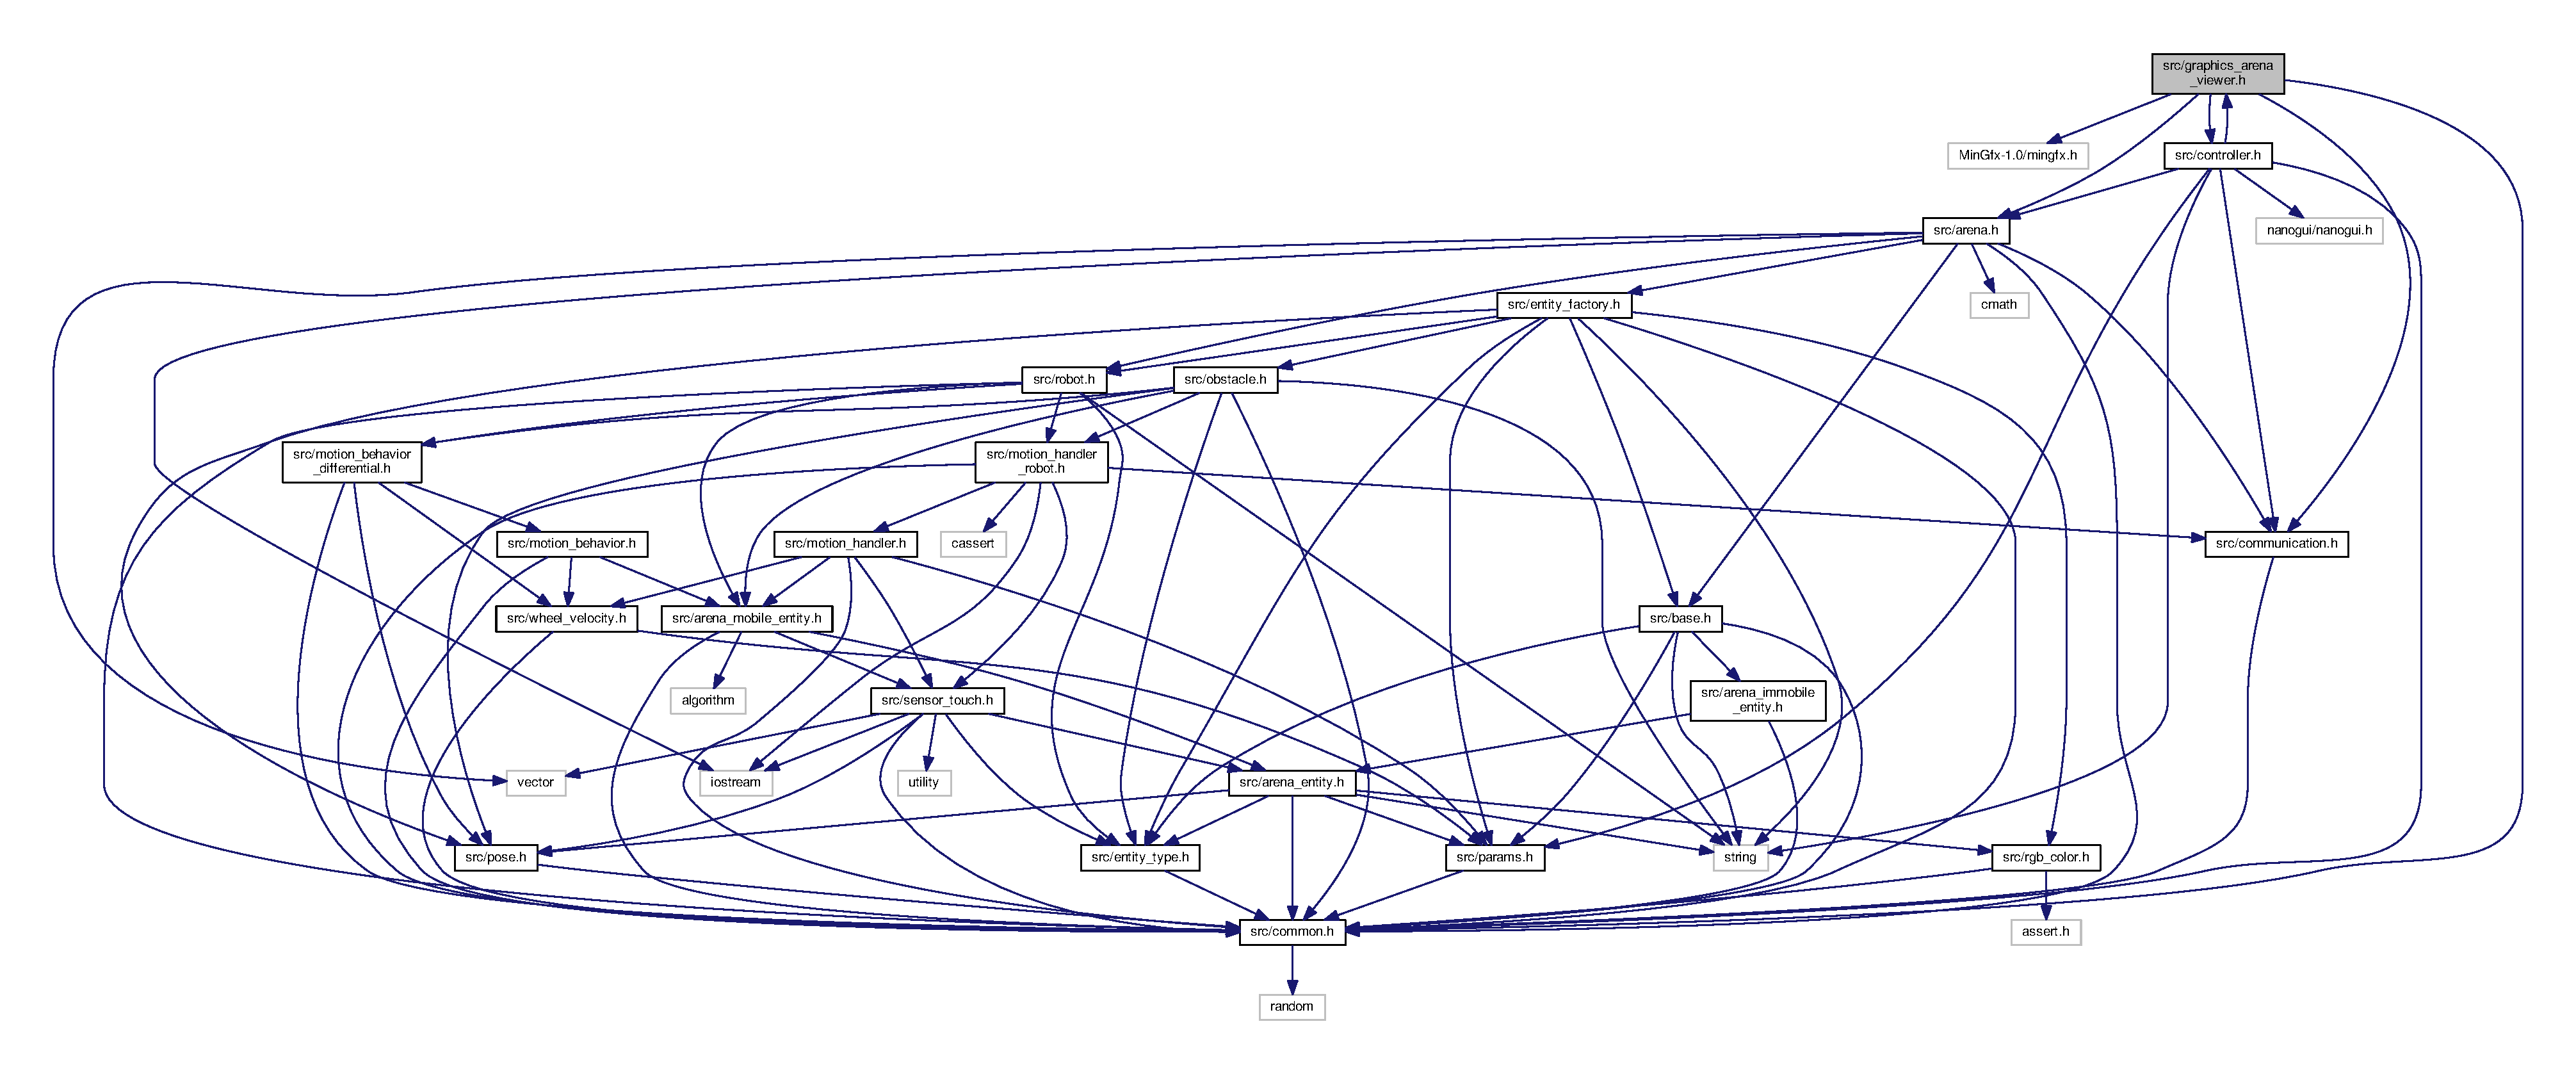
\includegraphics[width=350pt]{graphics__arena__viewer_8h__incl}
\end{center}
\end{figure}
This graph shows which files directly or indirectly include this file\+:
\nopagebreak
\begin{figure}[H]
\begin{center}
\leavevmode
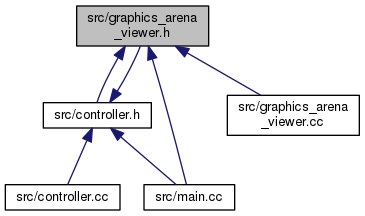
\includegraphics[width=350pt]{graphics__arena__viewer_8h__dep__incl}
\end{center}
\end{figure}
\subsection*{Classes}
\begin{DoxyCompactItemize}
\item 
class \hyperlink{classGraphicsArenaViewer}{Graphics\+Arena\+Viewer}
\begin{DoxyCompactList}\small\item\em An application that uses the Min\+Gfx library to open up a window that includes a few buttons for controlling the simulation and can be used to draw circles and other computer graphics. \end{DoxyCompactList}\end{DoxyCompactItemize}
\subsection*{Functions}
\begin{DoxyCompactItemize}
\item 
{\bfseries N\+A\+M\+E\+S\+P\+A\+C\+E\+\_\+\+B\+E\+G\+IN} (csci3081)\hypertarget{graphics__arena__viewer_8h_a5eaf22d0e7e2a0f12c6a660a6b011297}{}\label{graphics__arena__viewer_8h_a5eaf22d0e7e2a0f12c6a660a6b011297}

\item 
{\bfseries N\+A\+M\+E\+S\+P\+A\+C\+E\+\_\+\+E\+ND} (csci3081)\hypertarget{graphics__arena__viewer_8h_a0bc8eb973c3aef52acd7429898ace1cd}{}\label{graphics__arena__viewer_8h_a0bc8eb973c3aef52acd7429898ace1cd}

\end{DoxyCompactItemize}


\subsection{Detailed Description}
\begin{DoxyCopyright}{Copyright}
2017 3081 Staff, All rights reserved. 
\end{DoxyCopyright}

\hypertarget{light_8cc}{}\section{src/light.cc File Reference}
\label{light_8cc}\index{src/light.\+cc@{src/light.\+cc}}
{\ttfamily \#include \char`\"{}src/light.\+h\char`\"{}}\\*
{\ttfamily \#include \char`\"{}src/params.\+h\char`\"{}}\\*
\subsection*{Functions}
\begin{DoxyCompactItemize}
\item 
{\bfseries N\+A\+M\+E\+S\+P\+A\+C\+E\+\_\+\+B\+E\+G\+IN} (csci3081)\hypertarget{light_8cc_a5eaf22d0e7e2a0f12c6a660a6b011297}{}\label{light_8cc_a5eaf22d0e7e2a0f12c6a660a6b011297}

\item 
{\bfseries N\+A\+M\+E\+S\+P\+A\+C\+E\+\_\+\+E\+ND} (csci3081)\hypertarget{light_8cc_a0bc8eb973c3aef52acd7429898ace1cd}{}\label{light_8cc_a0bc8eb973c3aef52acd7429898ace1cd}

\end{DoxyCompactItemize}


\subsection{Detailed Description}
\begin{DoxyCopyright}{Copyright}
2017 3081 Staff, All rights reserved. 
\end{DoxyCopyright}

\hypertarget{light_8h}{}\section{/home/musex025/\+Desktop/project-\/musex025/iteration2/src/light.h File Reference}
\label{light_8h}\index{/home/musex025/\+Desktop/project-\/musex025/iteration2/src/light.\+h@{/home/musex025/\+Desktop/project-\/musex025/iteration2/src/light.\+h}}
{\ttfamily \#include $<$string$>$}\\*
{\ttfamily \#include \char`\"{}src/arena\+\_\+mobile\+\_\+entity.\+h\char`\"{}}\\*
{\ttfamily \#include \char`\"{}src/common.\+h\char`\"{}}\\*
{\ttfamily \#include \char`\"{}src/entity\+\_\+type.\+h\char`\"{}}\\*
{\ttfamily \#include \char`\"{}src/pose.\+h\char`\"{}}\\*
{\ttfamily \#include \char`\"{}src/motion\+\_\+handler\+\_\+robot.\+h\char`\"{}}\\*
{\ttfamily \#include \char`\"{}src/motion\+\_\+behavior\+\_\+differential.\+h\char`\"{}}\\*
Include dependency graph for light.\+h\+:\nopagebreak
\begin{figure}[H]
\begin{center}
\leavevmode
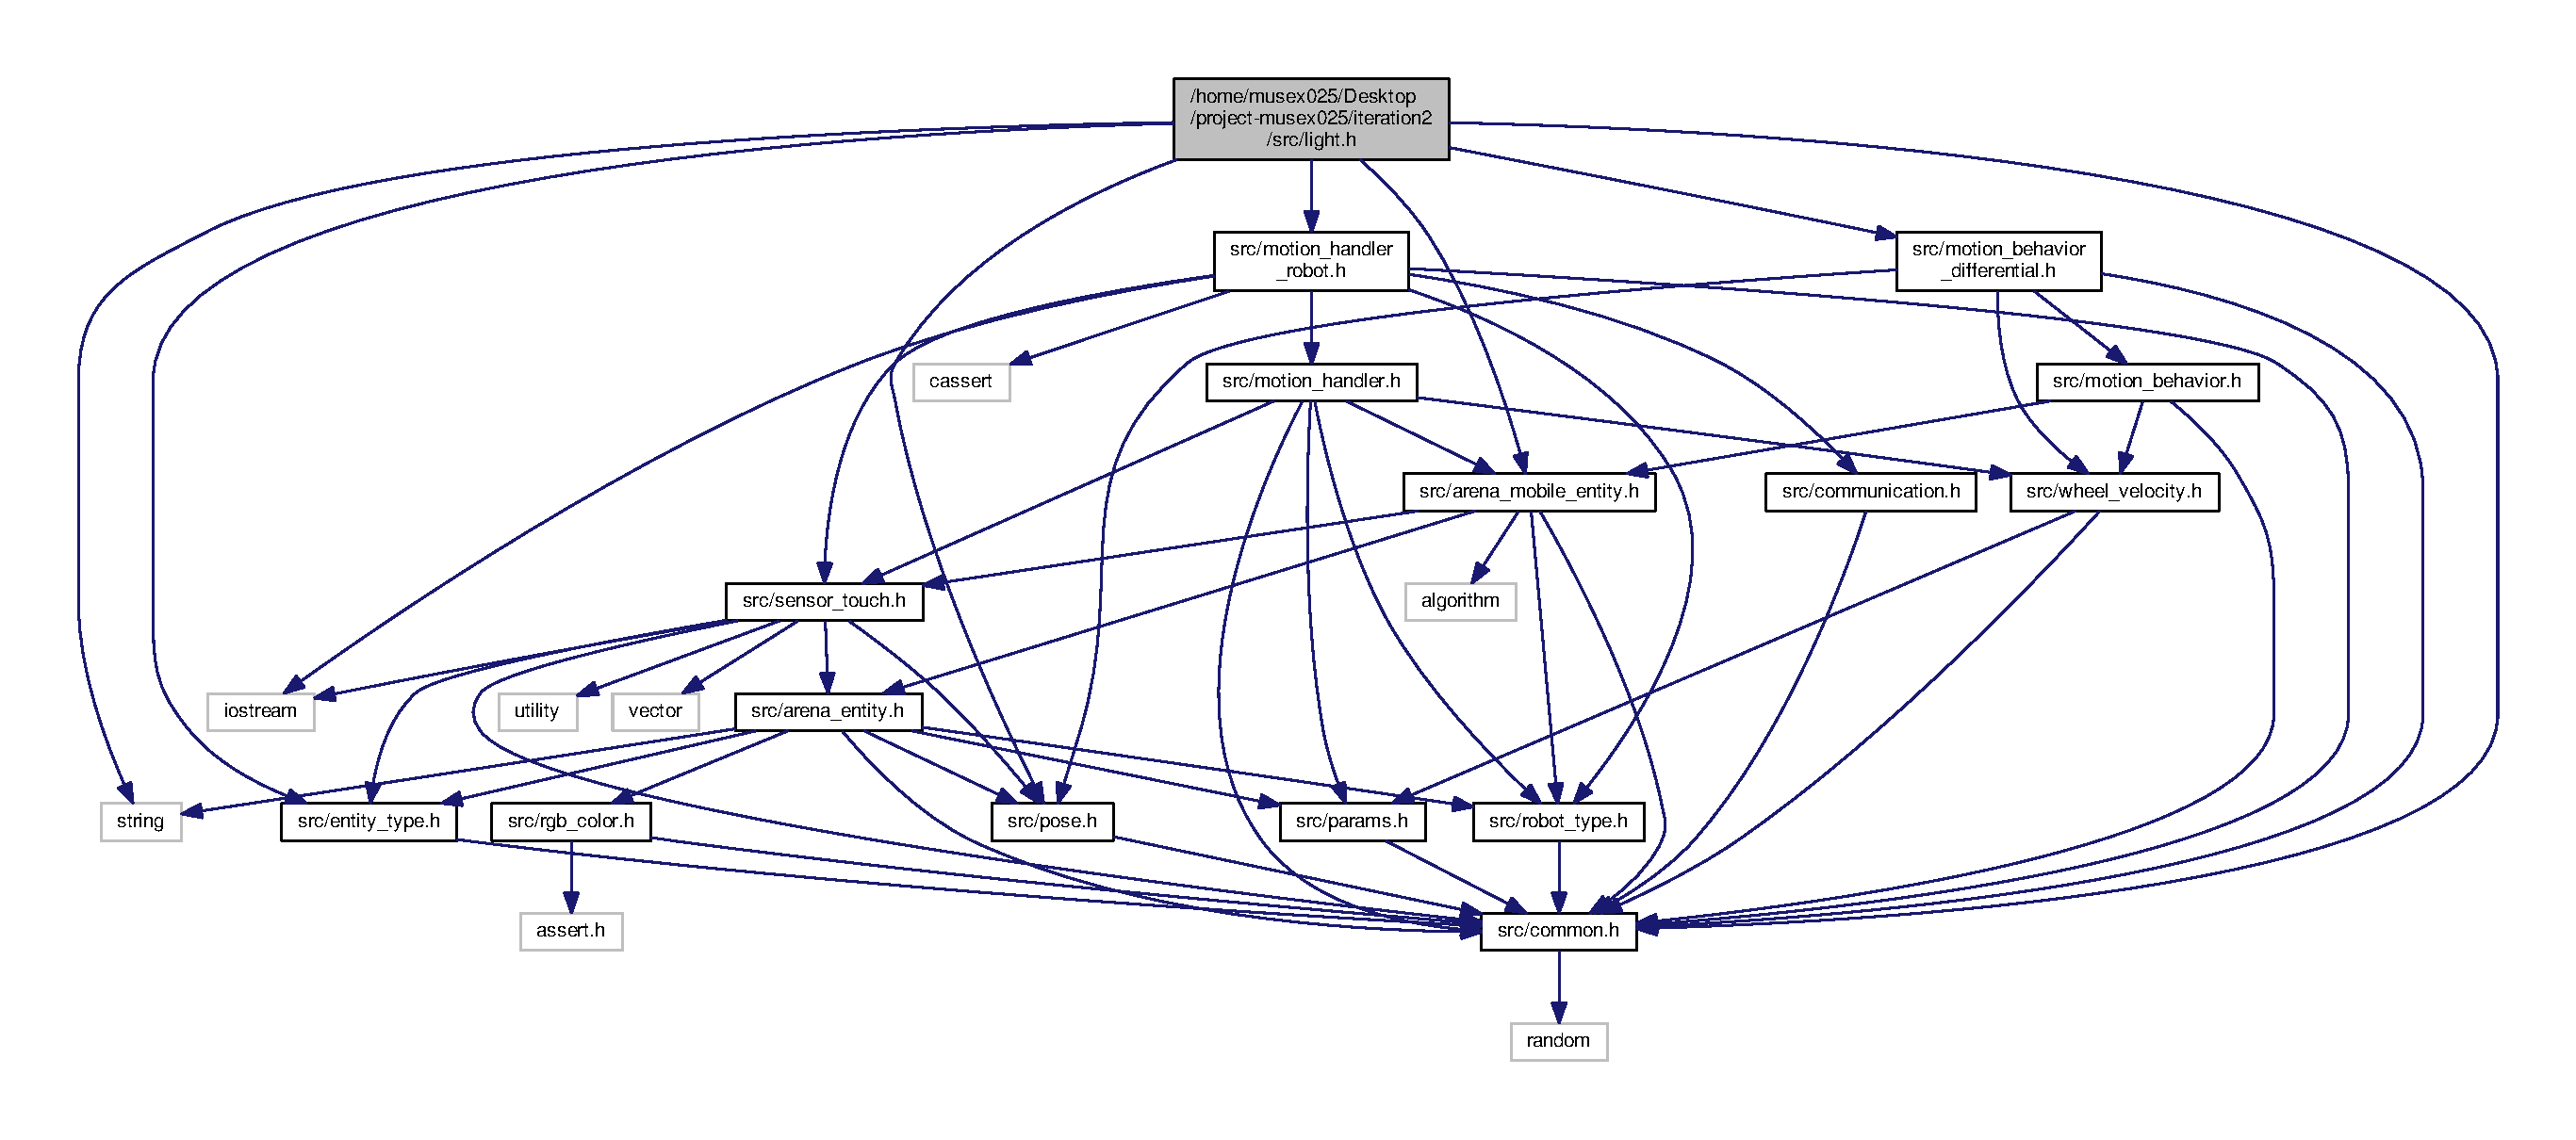
\includegraphics[width=350pt]{light_8h__incl}
\end{center}
\end{figure}
This graph shows which files directly or indirectly include this file\+:\nopagebreak
\begin{figure}[H]
\begin{center}
\leavevmode
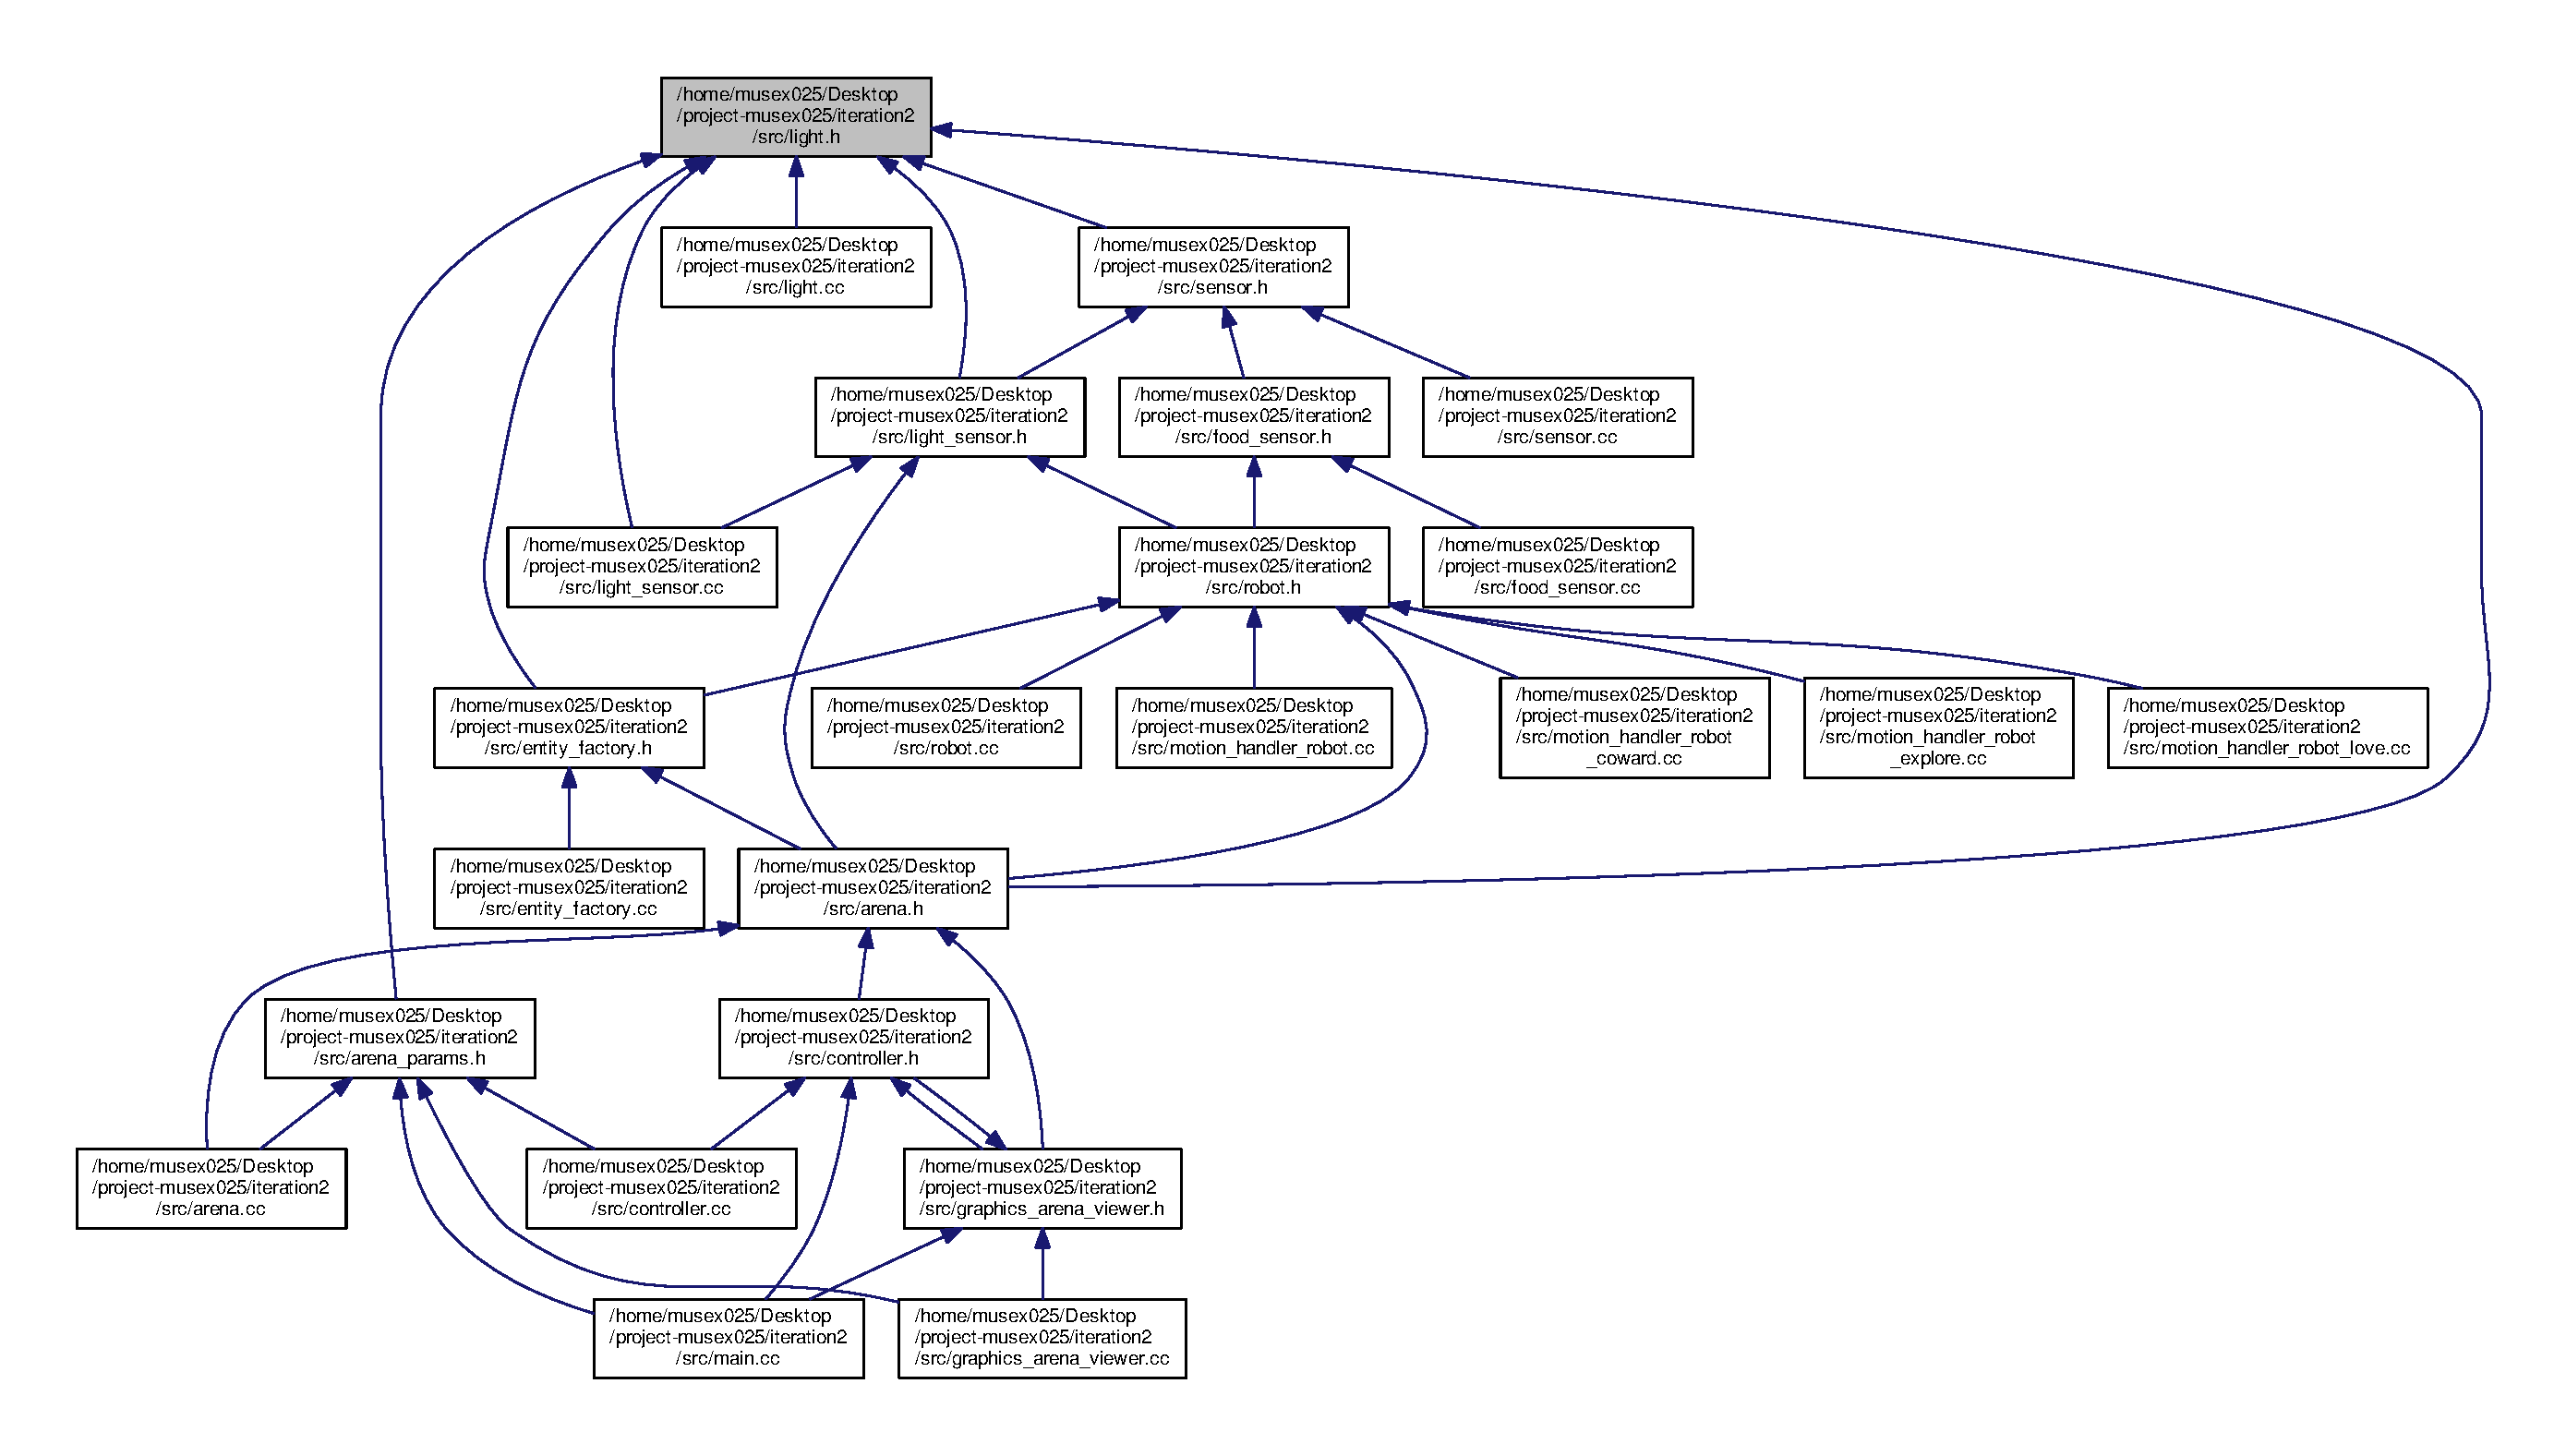
\includegraphics[width=350pt]{light_8h__dep__incl}
\end{center}
\end{figure}
\subsection*{Classes}
\begin{DoxyCompactItemize}
\item 
class \hyperlink{classLight}{Light}
\begin{DoxyCompactList}\small\item\em Class representing an mobile \hyperlink{classLight}{Light} within the \hyperlink{classArena}{Arena}. \end{DoxyCompactList}\end{DoxyCompactItemize}
\subsection*{Functions}
\begin{DoxyCompactItemize}
\item 
{\bfseries N\+A\+M\+E\+S\+P\+A\+C\+E\+\_\+\+B\+E\+G\+IN} (csci3081)\hypertarget{light_8h_a5eaf22d0e7e2a0f12c6a660a6b011297}{}\label{light_8h_a5eaf22d0e7e2a0f12c6a660a6b011297}

\item 
{\bfseries N\+A\+M\+E\+S\+P\+A\+C\+E\+\_\+\+E\+ND} (csci3081)\hypertarget{light_8h_a0bc8eb973c3aef52acd7429898ace1cd}{}\label{light_8h_a0bc8eb973c3aef52acd7429898ace1cd}

\end{DoxyCompactItemize}


\subsection{Detailed Description}
\begin{DoxyCopyright}{Copyright}
2017 3081 Staff, All rights reserved. 
\end{DoxyCopyright}

\hypertarget{light__sensor_8cc}{}\section{/home/musex025/\+Desktop/project-\/musex025/iteration2/src/light\+\_\+sensor.cc File Reference}
\label{light__sensor_8cc}\index{/home/musex025/\+Desktop/project-\/musex025/iteration2/src/light\+\_\+sensor.\+cc@{/home/musex025/\+Desktop/project-\/musex025/iteration2/src/light\+\_\+sensor.\+cc}}
{\ttfamily \#include $<$math.\+h$>$}\\*
{\ttfamily \#include $<$vector$>$}\\*
{\ttfamily \#include \char`\"{}src/light\+\_\+sensor.\+h\char`\"{}}\\*
{\ttfamily \#include \char`\"{}src/light.\+h\char`\"{}}\\*
{\ttfamily \#include \char`\"{}src/params.\+h\char`\"{}}\\*
Include dependency graph for light\+\_\+sensor.\+cc\+:\nopagebreak
\begin{figure}[H]
\begin{center}
\leavevmode
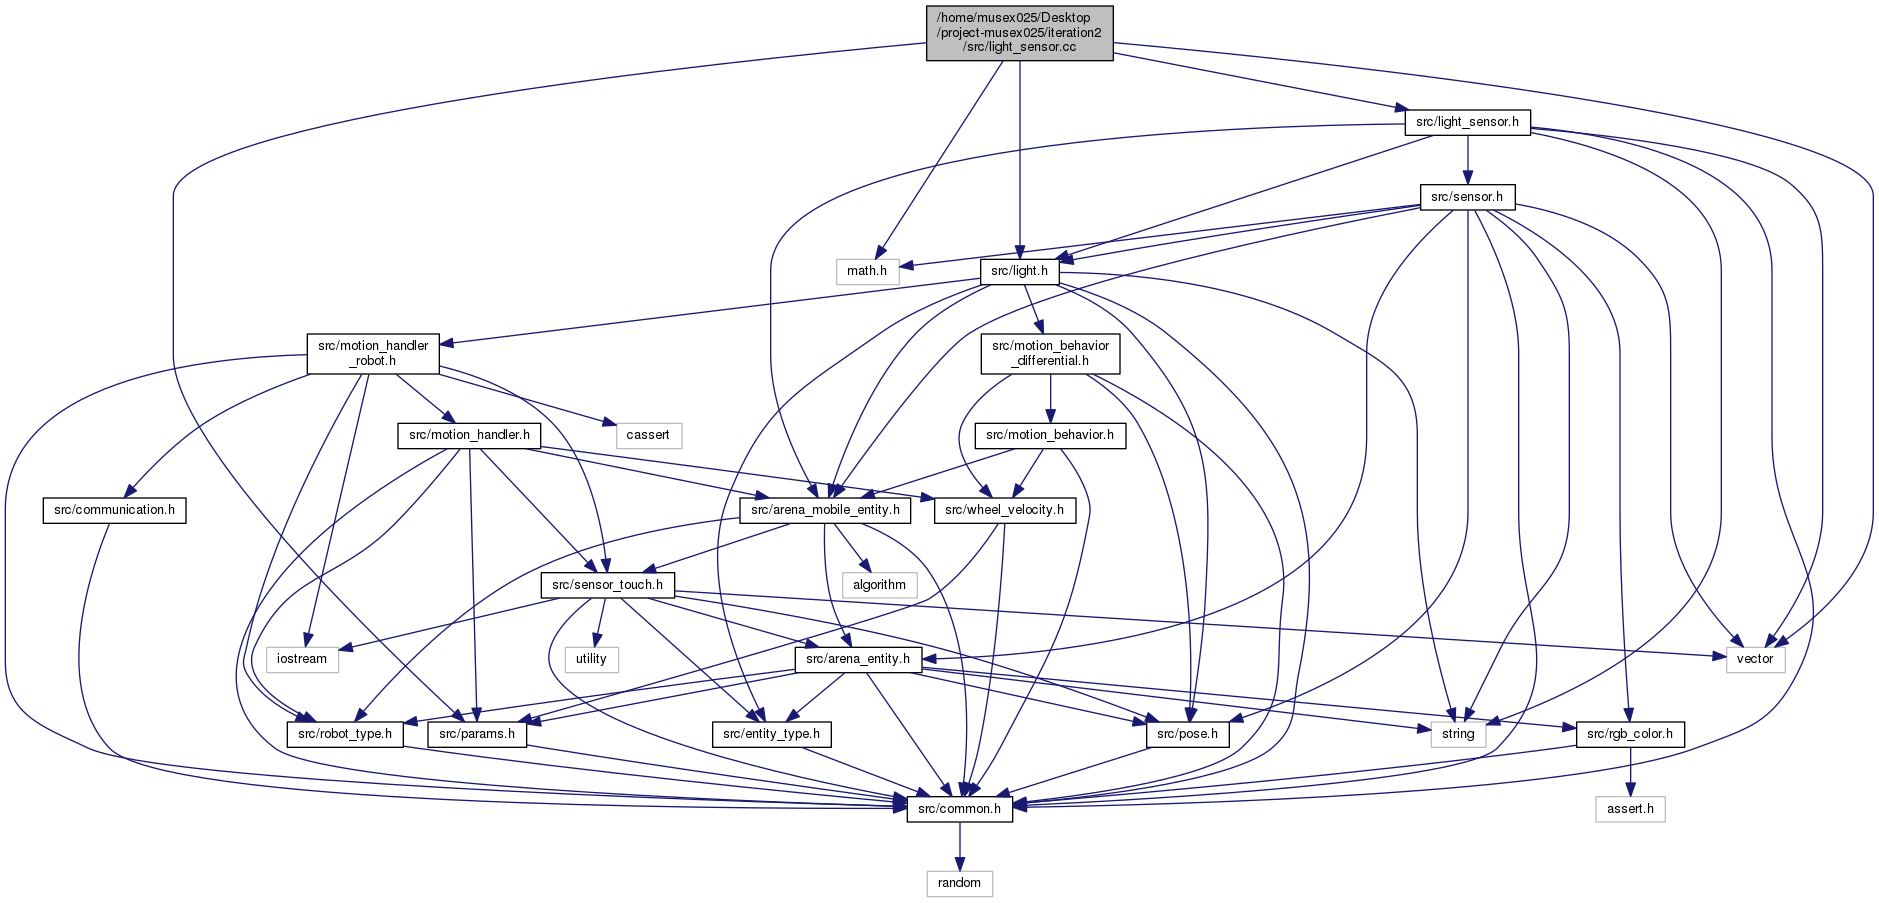
\includegraphics[width=350pt]{light__sensor_8cc__incl}
\end{center}
\end{figure}
\subsection*{Functions}
\begin{DoxyCompactItemize}
\item 
{\bfseries N\+A\+M\+E\+S\+P\+A\+C\+E\+\_\+\+B\+E\+G\+IN} (csci3081)\hypertarget{light__sensor_8cc_a5eaf22d0e7e2a0f12c6a660a6b011297}{}\label{light__sensor_8cc_a5eaf22d0e7e2a0f12c6a660a6b011297}

\item 
{\bfseries N\+A\+M\+E\+S\+P\+A\+C\+E\+\_\+\+E\+ND} (csci3081)\hypertarget{light__sensor_8cc_a0bc8eb973c3aef52acd7429898ace1cd}{}\label{light__sensor_8cc_a0bc8eb973c3aef52acd7429898ace1cd}

\end{DoxyCompactItemize}


\subsection{Detailed Description}
\begin{DoxyCopyright}{Copyright}
2017 3081 Staff, All rights reserved. 
\end{DoxyCopyright}

\hypertarget{light__sensor_8h}{}\section{src/light\+\_\+sensor.h File Reference}
\label{light__sensor_8h}\index{src/light\+\_\+sensor.\+h@{src/light\+\_\+sensor.\+h}}
{\ttfamily \#include $<$string$>$}\\*
{\ttfamily \#include $<$vector$>$}\\*
{\ttfamily \#include \char`\"{}src/common.\+h\char`\"{}}\\*
{\ttfamily \#include \char`\"{}src/sensor.\+h\char`\"{}}\\*
{\ttfamily \#include \char`\"{}src/light.\+h\char`\"{}}\\*
{\ttfamily \#include \char`\"{}src/arena\+\_\+mobile\+\_\+entity.\+h\char`\"{}}\\*
\subsection*{Classes}
\begin{DoxyCompactItemize}
\item 
class \hyperlink{class_light_sensor}{Light\+Sensor}
\end{DoxyCompactItemize}
\subsection*{Functions}
\begin{DoxyCompactItemize}
\item 
{\bfseries N\+A\+M\+E\+S\+P\+A\+C\+E\+\_\+\+B\+E\+G\+IN} (csci3081)\hypertarget{light__sensor_8h_a5eaf22d0e7e2a0f12c6a660a6b011297}{}\label{light__sensor_8h_a5eaf22d0e7e2a0f12c6a660a6b011297}

\item 
{\bfseries N\+A\+M\+E\+S\+P\+A\+C\+E\+\_\+\+E\+ND} (csci3081)\hypertarget{light__sensor_8h_a0bc8eb973c3aef52acd7429898ace1cd}{}\label{light__sensor_8h_a0bc8eb973c3aef52acd7429898ace1cd}

\end{DoxyCompactItemize}


\subsection{Detailed Description}
\begin{DoxyCopyright}{Copyright}
2017 3081 Staff, All rights reserved. 
\end{DoxyCopyright}

\hypertarget{main_8cc}{}\section{src/main.cc File Reference}
\label{main_8cc}\index{src/main.\+cc@{src/main.\+cc}}
{\ttfamily \#include $<$iostream$>$}\\*
{\ttfamily \#include \char`\"{}src/arena\+\_\+params.\+h\char`\"{}}\\*
{\ttfamily \#include \char`\"{}src/controller.\+h\char`\"{}}\\*
{\ttfamily \#include \char`\"{}src/graphics\+\_\+arena\+\_\+viewer.\+h\char`\"{}}\\*
Include dependency graph for main.\+cc\+:\nopagebreak
\begin{figure}[H]
\begin{center}
\leavevmode
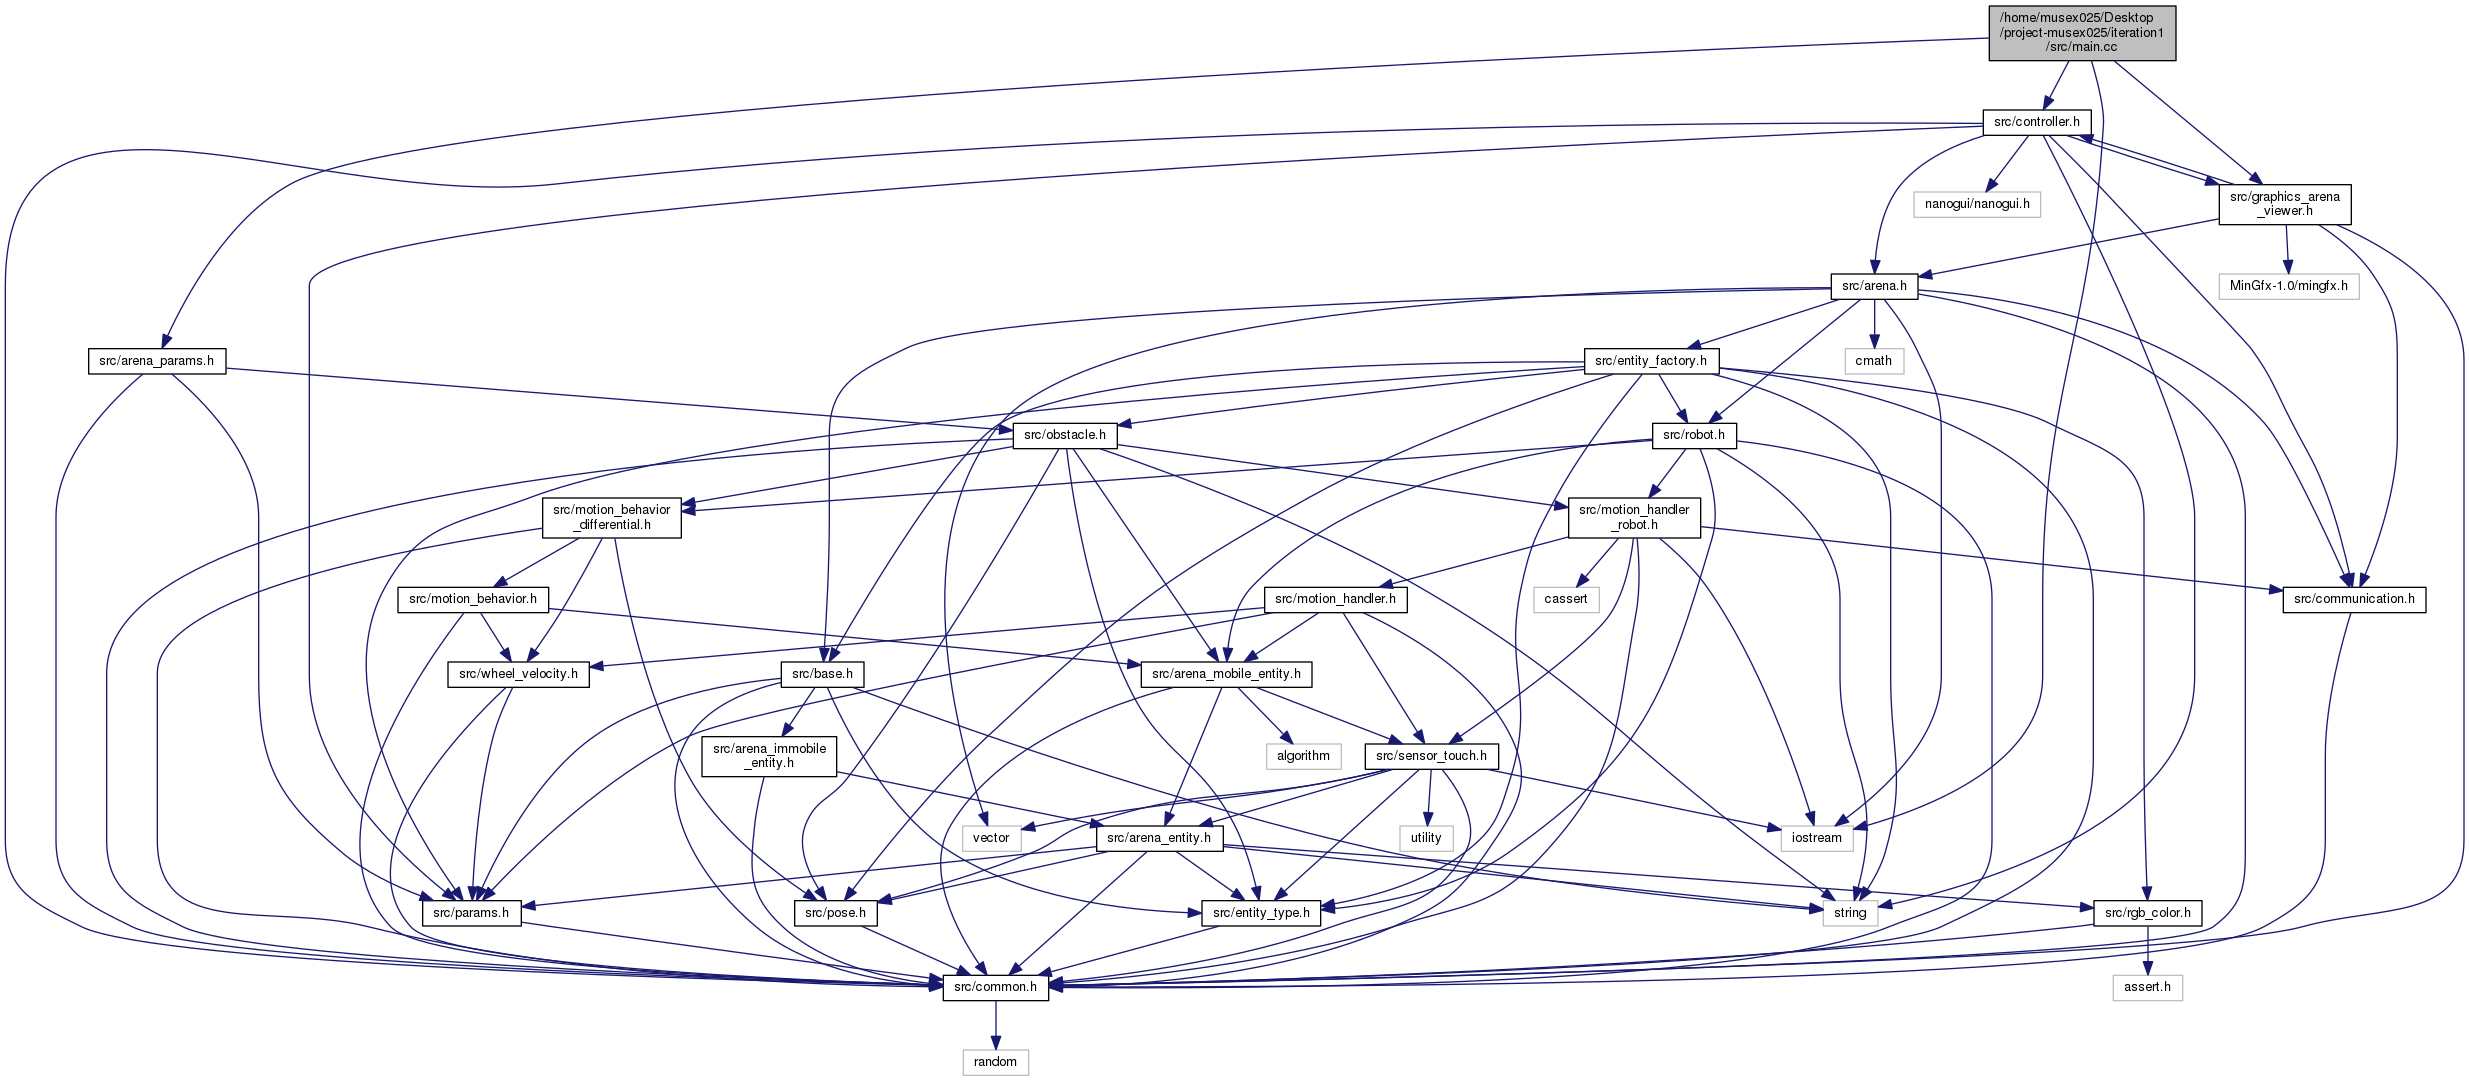
\includegraphics[width=350pt]{main_8cc__incl}
\end{center}
\end{figure}
\subsection*{Functions}
\begin{DoxyCompactItemize}
\item 
int {\bfseries main} (\hyperlink{common_8h_a2e3484535ee610c8e19e9859563abe48}{\+\_\+\+\_\+unused} int argc, \hyperlink{common_8h_a2e3484535ee610c8e19e9859563abe48}{\+\_\+\+\_\+unused} char $\ast$$\ast$argv)\hypertarget{main_8cc_a37539ad52260bcf576f148e7e141d4f2}{}\label{main_8cc_a37539ad52260bcf576f148e7e141d4f2}

\end{DoxyCompactItemize}


\subsection{Detailed Description}
\begin{DoxyCopyright}{Copyright}
2017 3081 Staff, All rights reserved. 
\end{DoxyCopyright}

\hypertarget{mainpage_8h}{}\section{/home/musex025/\+Desktop/project-\/musex025/iteration2/src/mainpage.h File Reference}
\label{mainpage_8h}\index{/home/musex025/\+Desktop/project-\/musex025/iteration2/src/mainpage.\+h@{/home/musex025/\+Desktop/project-\/musex025/iteration2/src/mainpage.\+h}}


\subsection{Detailed Description}
\begin{DoxyCopyright}{Copyright}
2017 3081 Staff, All rights reserved. 
\end{DoxyCopyright}

\hypertarget{motion__behavior_8cc}{}\section{/home/musex025/\+Desktop/project-\/musex025/iteration2/src/motion\+\_\+behavior.cc File Reference}
\label{motion__behavior_8cc}\index{/home/musex025/\+Desktop/project-\/musex025/iteration2/src/motion\+\_\+behavior.\+cc@{/home/musex025/\+Desktop/project-\/musex025/iteration2/src/motion\+\_\+behavior.\+cc}}
{\ttfamily \#include $<$iostream$>$}\\*
{\ttfamily \#include \char`\"{}src/motion\+\_\+behavior.\+h\char`\"{}}\\*
{\ttfamily \#include \char`\"{}src/arena\+\_\+mobile\+\_\+entity.\+h\char`\"{}}\\*
{\ttfamily \#include \char`\"{}src/entity\+\_\+type.\+h\char`\"{}}\\*
Include dependency graph for motion\+\_\+behavior.\+cc\+:\nopagebreak
\begin{figure}[H]
\begin{center}
\leavevmode
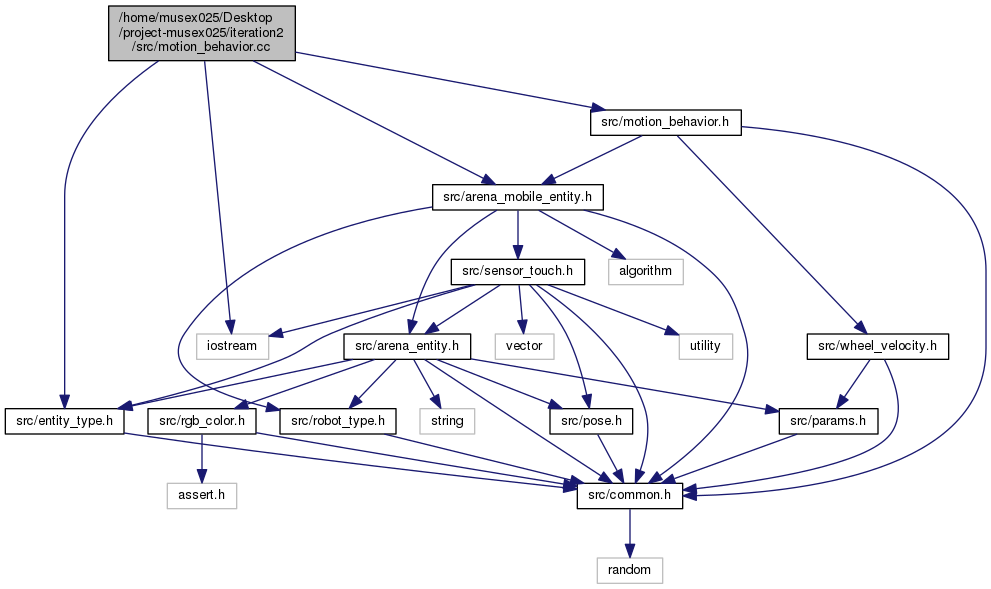
\includegraphics[width=350pt]{motion__behavior_8cc__incl}
\end{center}
\end{figure}
\subsection*{Functions}
\begin{DoxyCompactItemize}
\item 
{\bfseries N\+A\+M\+E\+S\+P\+A\+C\+E\+\_\+\+B\+E\+G\+IN} (csci3081)\hypertarget{motion__behavior_8cc_a5eaf22d0e7e2a0f12c6a660a6b011297}{}\label{motion__behavior_8cc_a5eaf22d0e7e2a0f12c6a660a6b011297}

\item 
{\bfseries N\+A\+M\+E\+S\+P\+A\+C\+E\+\_\+\+E\+ND} (csci3081)\hypertarget{motion__behavior_8cc_a0bc8eb973c3aef52acd7429898ace1cd}{}\label{motion__behavior_8cc_a0bc8eb973c3aef52acd7429898ace1cd}

\end{DoxyCompactItemize}


\subsection{Detailed Description}
\begin{DoxyCopyright}{Copyright}
2017 3081 Staff, All rights reserved. 
\end{DoxyCopyright}

\hypertarget{motion__behavior_8h}{}\section{src/motion\+\_\+behavior.h File Reference}
\label{motion__behavior_8h}\index{src/motion\+\_\+behavior.\+h@{src/motion\+\_\+behavior.\+h}}
{\ttfamily \#include \char`\"{}src/common.\+h\char`\"{}}\newline
{\ttfamily \#include \char`\"{}src/wheel\+\_\+velocity.\+h\char`\"{}}\newline
{\ttfamily \#include \char`\"{}src/arena\+\_\+mobile\+\_\+entity.\+h\char`\"{}}\newline
\subsection*{Classes}
\begin{DoxyCompactItemize}
\item 
class \mbox{\hyperlink{class_motion_behavior}{Motion\+Behavior}}
\begin{DoxyCompactList}\small\item\em Class managing an \mbox{\hyperlink{class_arena_mobile_entity}{Arena\+Mobile\+Entity}}\textquotesingle{}s position. \end{DoxyCompactList}\end{DoxyCompactItemize}
\subsection*{Functions}
\begin{DoxyCompactItemize}
\item 
\mbox{\Hypertarget{motion__behavior_8h_a5eaf22d0e7e2a0f12c6a660a6b011297}\label{motion__behavior_8h_a5eaf22d0e7e2a0f12c6a660a6b011297}} 
{\bfseries N\+A\+M\+E\+S\+P\+A\+C\+E\+\_\+\+B\+E\+G\+IN} (csci3081)
\item 
\mbox{\Hypertarget{motion__behavior_8h_a0bc8eb973c3aef52acd7429898ace1cd}\label{motion__behavior_8h_a0bc8eb973c3aef52acd7429898ace1cd}} 
{\bfseries N\+A\+M\+E\+S\+P\+A\+C\+E\+\_\+\+E\+ND} (csci3081)
\end{DoxyCompactItemize}


\subsection{Detailed Description}
\begin{DoxyCopyright}{Copyright}
2017 3081 Staff, All rights reserved. 
\end{DoxyCopyright}

\hypertarget{motion__behavior__differential_8h}{}\section{src/motion\+\_\+behavior\+\_\+differential.h File Reference}
\label{motion__behavior__differential_8h}\index{src/motion\+\_\+behavior\+\_\+differential.\+h@{src/motion\+\_\+behavior\+\_\+differential.\+h}}
{\ttfamily \#include \char`\"{}src/common.\+h\char`\"{}}\newline
{\ttfamily \#include \char`\"{}src/pose.\+h\char`\"{}}\newline
{\ttfamily \#include \char`\"{}src/wheel\+\_\+velocity.\+h\char`\"{}}\newline
{\ttfamily \#include \char`\"{}src/motion\+\_\+behavior.\+h\char`\"{}}\newline
\subsection*{Classes}
\begin{DoxyCompactItemize}
\item 
class \mbox{\hyperlink{class_motion_behavior_differential}{Motion\+Behavior\+Differential}}
\begin{DoxyCompactList}\small\item\em A simple model of differential drive kinematics based on the notes here\+: $\sim$https\+://chess.eecs.\+berkeley.\+edu/eecs149/documentation/differential\+Drive.pdf$\sim$. \end{DoxyCompactList}\end{DoxyCompactItemize}
\subsection*{Functions}
\begin{DoxyCompactItemize}
\item 
\mbox{\Hypertarget{motion__behavior__differential_8h_a5eaf22d0e7e2a0f12c6a660a6b011297}\label{motion__behavior__differential_8h_a5eaf22d0e7e2a0f12c6a660a6b011297}} 
{\bfseries N\+A\+M\+E\+S\+P\+A\+C\+E\+\_\+\+B\+E\+G\+IN} (csci3081)
\item 
\mbox{\Hypertarget{motion__behavior__differential_8h_a0bc8eb973c3aef52acd7429898ace1cd}\label{motion__behavior__differential_8h_a0bc8eb973c3aef52acd7429898ace1cd}} 
{\bfseries N\+A\+M\+E\+S\+P\+A\+C\+E\+\_\+\+E\+ND} (csci3081)
\end{DoxyCompactItemize}


\subsection{Detailed Description}
\begin{DoxyCopyright}{Copyright}
2018 3081 Staff, All rights reserved. 
\end{DoxyCopyright}

\hypertarget{motion__handler_8cc}{}\section{/home/musex025/\+Desktop/project-\/musex025/iteration1/src/motion\+\_\+handler.cc File Reference}
\label{motion__handler_8cc}\index{/home/musex025/\+Desktop/project-\/musex025/iteration1/src/motion\+\_\+handler.\+cc@{/home/musex025/\+Desktop/project-\/musex025/iteration1/src/motion\+\_\+handler.\+cc}}
{\ttfamily \#include \char`\"{}src/motion\+\_\+handler.\+h\char`\"{}}\\*
{\ttfamily \#include $<$iostream$>$}\\*
Include dependency graph for motion\+\_\+handler.\+cc\+:
\nopagebreak
\begin{figure}[H]
\begin{center}
\leavevmode
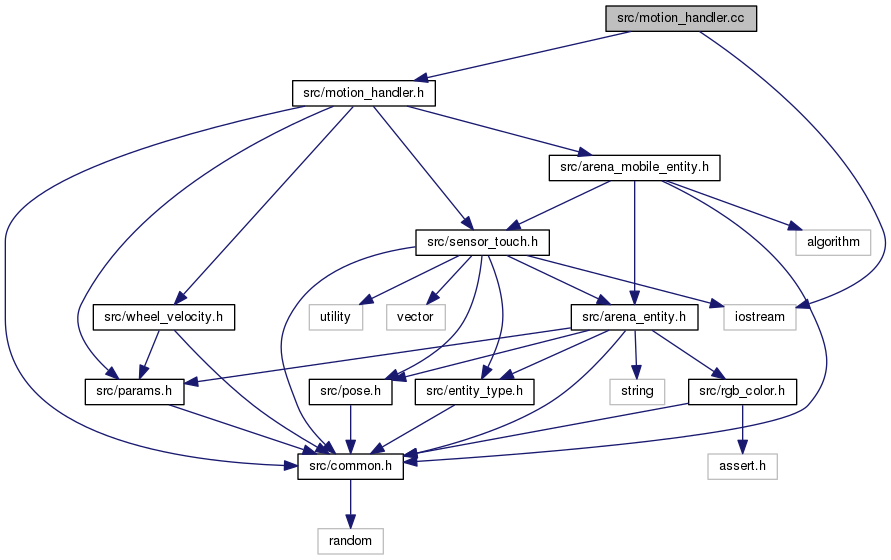
\includegraphics[width=350pt]{motion__handler_8cc__incl}
\end{center}
\end{figure}
\subsection*{Functions}
\begin{DoxyCompactItemize}
\item 
{\bfseries N\+A\+M\+E\+S\+P\+A\+C\+E\+\_\+\+B\+E\+G\+IN} (csci3081)\hypertarget{motion__handler_8cc_a5eaf22d0e7e2a0f12c6a660a6b011297}{}\label{motion__handler_8cc_a5eaf22d0e7e2a0f12c6a660a6b011297}

\item 
{\bfseries N\+A\+M\+E\+S\+P\+A\+C\+E\+\_\+\+E\+ND} (csci3081)\hypertarget{motion__handler_8cc_a0bc8eb973c3aef52acd7429898ace1cd}{}\label{motion__handler_8cc_a0bc8eb973c3aef52acd7429898ace1cd}

\end{DoxyCompactItemize}


\subsection{Detailed Description}
\begin{DoxyCopyright}{Copyright}
2017 3081 Staff, All rights reserved. 
\end{DoxyCopyright}

\hypertarget{motion__handler_8h}{}\section{src/motion\+\_\+handler.h File Reference}
\label{motion__handler_8h}\index{src/motion\+\_\+handler.\+h@{src/motion\+\_\+handler.\+h}}
{\ttfamily \#include \char`\"{}src/common.\+h\char`\"{}}\\*
{\ttfamily \#include \char`\"{}src/params.\+h\char`\"{}}\\*
{\ttfamily \#include \char`\"{}src/wheel\+\_\+velocity.\+h\char`\"{}}\\*
{\ttfamily \#include \char`\"{}src/sensor\+\_\+touch.\+h\char`\"{}}\\*
{\ttfamily \#include \char`\"{}src/arena\+\_\+mobile\+\_\+entity.\+h\char`\"{}}\\*
{\ttfamily \#include \char`\"{}src/robot\+\_\+type.\+h\char`\"{}}\\*
\subsection*{Classes}
\begin{DoxyCompactItemize}
\item 
class \hyperlink{class_motion_handler}{Motion\+Handler}
\begin{DoxyCompactList}\small\item\em Base class for managing the pose and wheel velocity of the entity. \end{DoxyCompactList}\end{DoxyCompactItemize}
\subsection*{Functions}
\begin{DoxyCompactItemize}
\item 
{\bfseries N\+A\+M\+E\+S\+P\+A\+C\+E\+\_\+\+B\+E\+G\+IN} (csci3081)\hypertarget{motion__handler_8h_a5eaf22d0e7e2a0f12c6a660a6b011297}{}\label{motion__handler_8h_a5eaf22d0e7e2a0f12c6a660a6b011297}

\item 
{\bfseries N\+A\+M\+E\+S\+P\+A\+C\+E\+\_\+\+E\+ND} (csci3081)\hypertarget{motion__handler_8h_a0bc8eb973c3aef52acd7429898ace1cd}{}\label{motion__handler_8h_a0bc8eb973c3aef52acd7429898ace1cd}

\end{DoxyCompactItemize}


\subsection{Detailed Description}
\begin{DoxyCopyright}{Copyright}
2017 3081 Staff, All rights reserved. 
\end{DoxyCopyright}

\hypertarget{motion__handler__robot_8cc}{}\section{src/motion\+\_\+handler\+\_\+robot.cc File Reference}
\label{motion__handler__robot_8cc}\index{src/motion\+\_\+handler\+\_\+robot.\+cc@{src/motion\+\_\+handler\+\_\+robot.\+cc}}
{\ttfamily \#include \char`\"{}src/motion\+\_\+handler\+\_\+robot.\+h\char`\"{}}\newline
{\ttfamily \#include \char`\"{}src/motion\+\_\+behavior\+\_\+differential.\+h\char`\"{}}\newline
{\ttfamily \#include \char`\"{}src/robot.\+h\char`\"{}}\newline
{\ttfamily \#include \char`\"{}src/robot\+\_\+type.\+h\char`\"{}}\newline
\subsection*{Functions}
\begin{DoxyCompactItemize}
\item 
\mbox{\Hypertarget{motion__handler__robot_8cc_a5eaf22d0e7e2a0f12c6a660a6b011297}\label{motion__handler__robot_8cc_a5eaf22d0e7e2a0f12c6a660a6b011297}} 
{\bfseries N\+A\+M\+E\+S\+P\+A\+C\+E\+\_\+\+B\+E\+G\+IN} (csci3081)
\item 
\mbox{\Hypertarget{motion__handler__robot_8cc_a0bc8eb973c3aef52acd7429898ace1cd}\label{motion__handler__robot_8cc_a0bc8eb973c3aef52acd7429898ace1cd}} 
{\bfseries N\+A\+M\+E\+S\+P\+A\+C\+E\+\_\+\+E\+ND} (csci3081)
\end{DoxyCompactItemize}


\subsection{Detailed Description}
\begin{DoxyCopyright}{Copyright}
2018 3081 Staff, All rights reserved. 
\end{DoxyCopyright}

\hypertarget{motion__handler__robot_8h}{}\section{src/motion\+\_\+handler\+\_\+robot.h File Reference}
\label{motion__handler__robot_8h}\index{src/motion\+\_\+handler\+\_\+robot.\+h@{src/motion\+\_\+handler\+\_\+robot.\+h}}
{\ttfamily \#include $<$cassert$>$}\newline
{\ttfamily \#include $<$iostream$>$}\newline
{\ttfamily \#include \char`\"{}src/common.\+h\char`\"{}}\newline
{\ttfamily \#include \char`\"{}src/motion\+\_\+handler.\+h\char`\"{}}\newline
{\ttfamily \#include \char`\"{}src/sensor\+\_\+touch.\+h\char`\"{}}\newline
{\ttfamily \#include \char`\"{}src/communication.\+h\char`\"{}}\newline
{\ttfamily \#include \char`\"{}src/robot\+\_\+type.\+h\char`\"{}}\newline
\subsection*{Classes}
\begin{DoxyCompactItemize}
\item 
class \mbox{\hyperlink{class_motion_handler_robot}{Motion\+Handler\+Robot}}
\begin{DoxyCompactList}\small\item\em Class managing a \mbox{\hyperlink{class_robot}{Robot}}\textquotesingle{}s and \mbox{\hyperlink{class_light}{Light}}\textquotesingle{}s speed and heading angle based on collisions and user inputs. \end{DoxyCompactList}\end{DoxyCompactItemize}
\subsection*{Functions}
\begin{DoxyCompactItemize}
\item 
\mbox{\Hypertarget{motion__handler__robot_8h_a5eaf22d0e7e2a0f12c6a660a6b011297}\label{motion__handler__robot_8h_a5eaf22d0e7e2a0f12c6a660a6b011297}} 
{\bfseries N\+A\+M\+E\+S\+P\+A\+C\+E\+\_\+\+B\+E\+G\+IN} (csci3081)
\item 
\mbox{\Hypertarget{motion__handler__robot_8h_a0bc8eb973c3aef52acd7429898ace1cd}\label{motion__handler__robot_8h_a0bc8eb973c3aef52acd7429898ace1cd}} 
{\bfseries N\+A\+M\+E\+S\+P\+A\+C\+E\+\_\+\+E\+ND} (csci3081)
\end{DoxyCompactItemize}


\subsection{Detailed Description}
\begin{DoxyCopyright}{Copyright}
2018 3081 Staff, All rights reserved. 
\end{DoxyCopyright}

\hypertarget{motion__handler__robot__aggressive_8cc}{}\section{src/motion\+\_\+handler\+\_\+robot\+\_\+aggressive.cc File Reference}
\label{motion__handler__robot__aggressive_8cc}\index{src/motion\+\_\+handler\+\_\+robot\+\_\+aggressive.\+cc@{src/motion\+\_\+handler\+\_\+robot\+\_\+aggressive.\+cc}}
{\ttfamily \#include \char`\"{}src/motion\+\_\+handler\+\_\+robot\+\_\+aggressive.\+h\char`\"{}}\newline
{\ttfamily \#include \char`\"{}src/motion\+\_\+behavior\+\_\+differential.\+h\char`\"{}}\newline
{\ttfamily \#include \char`\"{}src/robot.\+h\char`\"{}}\newline
{\ttfamily \#include \char`\"{}src/robot\+\_\+type.\+h\char`\"{}}\newline
\subsection*{Functions}
\begin{DoxyCompactItemize}
\item 
\mbox{\Hypertarget{motion__handler__robot__aggressive_8cc_a5eaf22d0e7e2a0f12c6a660a6b011297}\label{motion__handler__robot__aggressive_8cc_a5eaf22d0e7e2a0f12c6a660a6b011297}} 
{\bfseries N\+A\+M\+E\+S\+P\+A\+C\+E\+\_\+\+B\+E\+G\+IN} (csci3081)
\item 
\mbox{\Hypertarget{motion__handler__robot__aggressive_8cc_a0bc8eb973c3aef52acd7429898ace1cd}\label{motion__handler__robot__aggressive_8cc_a0bc8eb973c3aef52acd7429898ace1cd}} 
{\bfseries N\+A\+M\+E\+S\+P\+A\+C\+E\+\_\+\+E\+ND} (csci3081)
\end{DoxyCompactItemize}


\subsection{Detailed Description}
\begin{DoxyCopyright}{Copyright}
2018 3081 Staff, All rights reserved. 
\end{DoxyCopyright}

\hypertarget{motion__handler__robot__aggressive_8h}{}\section{src/motion\+\_\+handler\+\_\+robot\+\_\+aggressive.h File Reference}
\label{motion__handler__robot__aggressive_8h}\index{src/motion\+\_\+handler\+\_\+robot\+\_\+aggressive.\+h@{src/motion\+\_\+handler\+\_\+robot\+\_\+aggressive.\+h}}
{\ttfamily \#include $<$cassert$>$}\\*
{\ttfamily \#include $<$iostream$>$}\\*
{\ttfamily \#include \char`\"{}src/common.\+h\char`\"{}}\\*
{\ttfamily \#include \char`\"{}src/motion\+\_\+handler.\+h\char`\"{}}\\*
{\ttfamily \#include \char`\"{}src/sensor\+\_\+touch.\+h\char`\"{}}\\*
{\ttfamily \#include \char`\"{}src/communication.\+h\char`\"{}}\\*
{\ttfamily \#include \char`\"{}src/robot\+\_\+type.\+h\char`\"{}}\\*
\subsection*{Classes}
\begin{DoxyCompactItemize}
\item 
class \hyperlink{class_motion_handler_robot_aggressive}{Motion\+Handler\+Robot\+Aggressive}
\begin{DoxyCompactList}\small\item\em Class managing a \hyperlink{class_robot}{Robot}\textquotesingle{}s and \hyperlink{class_light}{Light}\textquotesingle{}s speed and heading angle based on aggressive sensor readings. \end{DoxyCompactList}\end{DoxyCompactItemize}
\subsection*{Functions}
\begin{DoxyCompactItemize}
\item 
{\bfseries N\+A\+M\+E\+S\+P\+A\+C\+E\+\_\+\+B\+E\+G\+IN} (csci3081)\hypertarget{motion__handler__robot__aggressive_8h_a5eaf22d0e7e2a0f12c6a660a6b011297}{}\label{motion__handler__robot__aggressive_8h_a5eaf22d0e7e2a0f12c6a660a6b011297}

\item 
{\bfseries N\+A\+M\+E\+S\+P\+A\+C\+E\+\_\+\+E\+ND} (csci3081)\hypertarget{motion__handler__robot__aggressive_8h_a0bc8eb973c3aef52acd7429898ace1cd}{}\label{motion__handler__robot__aggressive_8h_a0bc8eb973c3aef52acd7429898ace1cd}

\end{DoxyCompactItemize}


\subsection{Detailed Description}
\begin{DoxyCopyright}{Copyright}
2018 3081 Staff, All rights reserved. 
\end{DoxyCopyright}

\hypertarget{motion__handler__robot__coward_8cc}{}\section{/home/musex025/\+Desktop/project-\/musex025/iteration2/src/motion\+\_\+handler\+\_\+robot\+\_\+coward.cc File Reference}
\label{motion__handler__robot__coward_8cc}\index{/home/musex025/\+Desktop/project-\/musex025/iteration2/src/motion\+\_\+handler\+\_\+robot\+\_\+coward.\+cc@{/home/musex025/\+Desktop/project-\/musex025/iteration2/src/motion\+\_\+handler\+\_\+robot\+\_\+coward.\+cc}}
{\ttfamily \#include \char`\"{}src/motion\+\_\+handler\+\_\+robot\+\_\+coward.\+h\char`\"{}}\\*
{\ttfamily \#include \char`\"{}src/motion\+\_\+behavior\+\_\+differential.\+h\char`\"{}}\\*
{\ttfamily \#include \char`\"{}src/robot.\+h\char`\"{}}\\*
{\ttfamily \#include \char`\"{}src/robot\+\_\+type.\+h\char`\"{}}\\*
Include dependency graph for motion\+\_\+handler\+\_\+robot\+\_\+coward.\+cc\+:\nopagebreak
\begin{figure}[H]
\begin{center}
\leavevmode
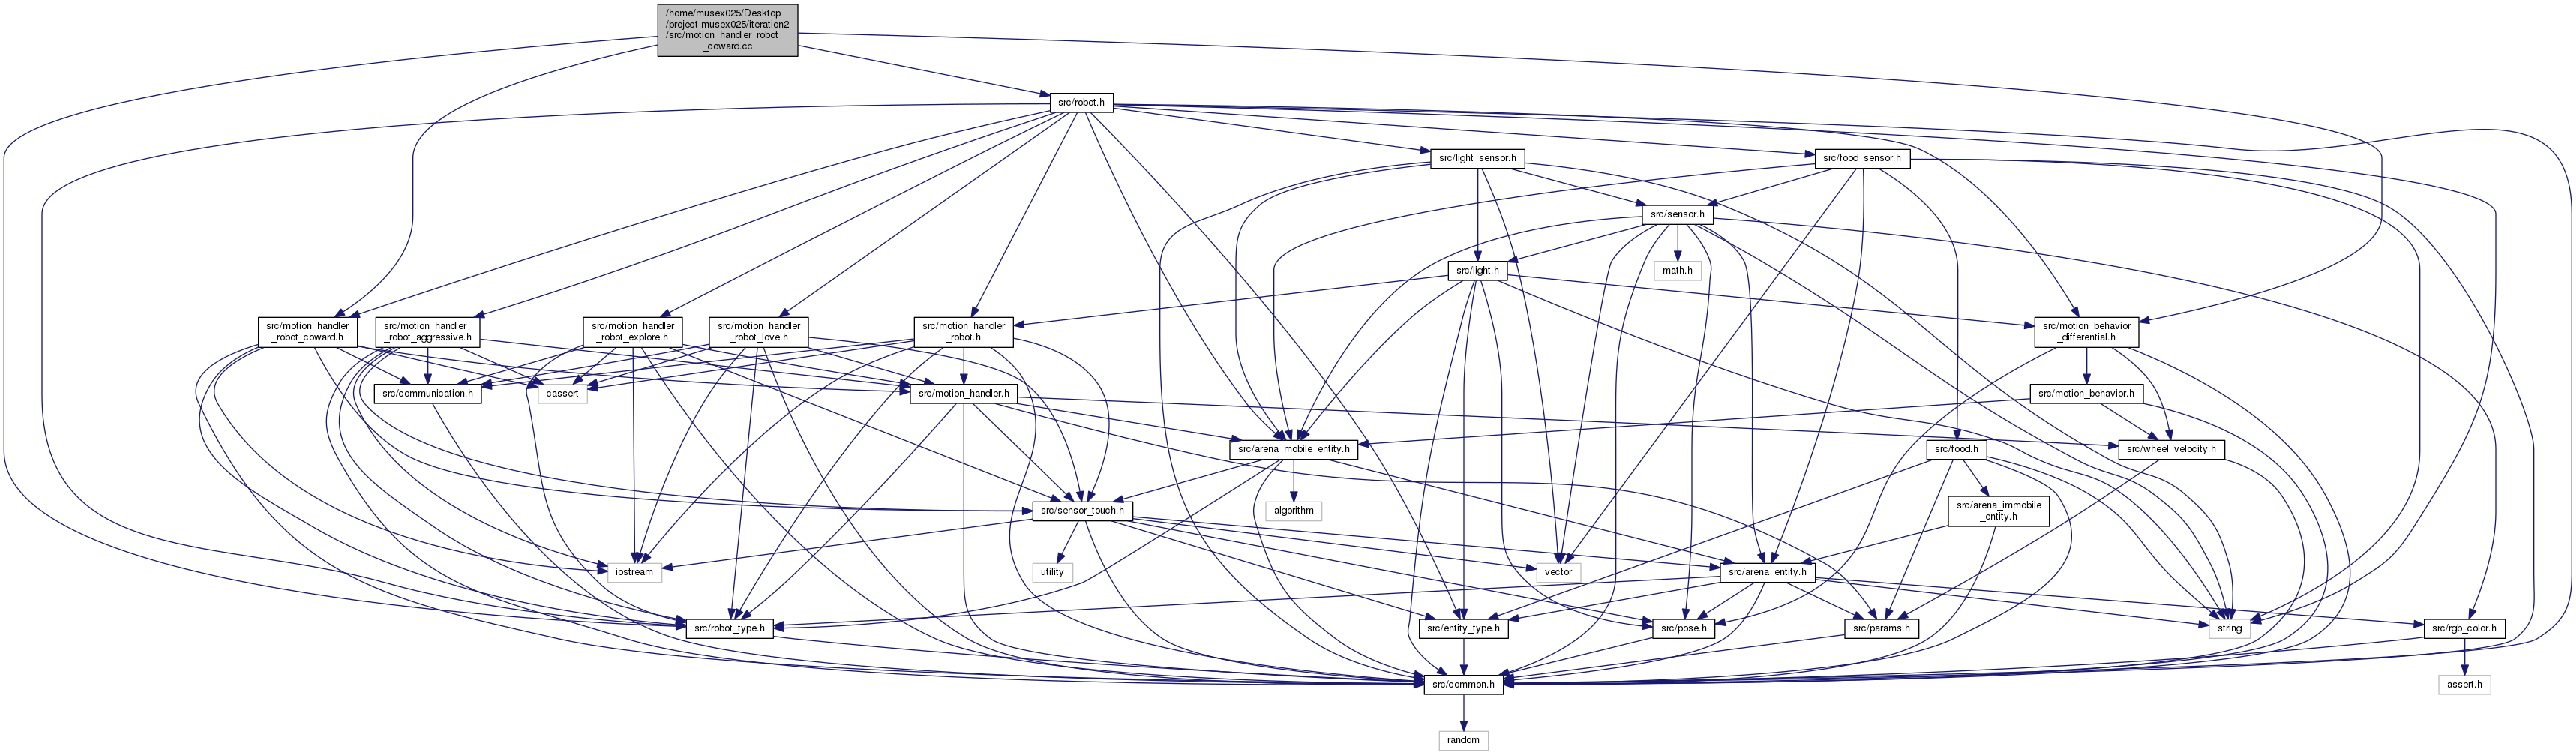
\includegraphics[width=350pt]{motion__handler__robot__coward_8cc__incl}
\end{center}
\end{figure}
\subsection*{Functions}
\begin{DoxyCompactItemize}
\item 
{\bfseries N\+A\+M\+E\+S\+P\+A\+C\+E\+\_\+\+B\+E\+G\+IN} (csci3081)\hypertarget{motion__handler__robot__coward_8cc_a5eaf22d0e7e2a0f12c6a660a6b011297}{}\label{motion__handler__robot__coward_8cc_a5eaf22d0e7e2a0f12c6a660a6b011297}

\item 
{\bfseries N\+A\+M\+E\+S\+P\+A\+C\+E\+\_\+\+E\+ND} (csci3081)\hypertarget{motion__handler__robot__coward_8cc_a0bc8eb973c3aef52acd7429898ace1cd}{}\label{motion__handler__robot__coward_8cc_a0bc8eb973c3aef52acd7429898ace1cd}

\end{DoxyCompactItemize}


\subsection{Detailed Description}
\begin{DoxyCopyright}{Copyright}
2018 3081 Staff, All rights reserved. 
\end{DoxyCopyright}

\hypertarget{motion__handler__robot__coward_8h}{}\section{/home/musex025/\+Desktop/project-\/musex025/iteration2/src/motion\+\_\+handler\+\_\+robot\+\_\+coward.h File Reference}
\label{motion__handler__robot__coward_8h}\index{/home/musex025/\+Desktop/project-\/musex025/iteration2/src/motion\+\_\+handler\+\_\+robot\+\_\+coward.\+h@{/home/musex025/\+Desktop/project-\/musex025/iteration2/src/motion\+\_\+handler\+\_\+robot\+\_\+coward.\+h}}
{\ttfamily \#include $<$cassert$>$}\\*
{\ttfamily \#include $<$iostream$>$}\\*
{\ttfamily \#include \char`\"{}src/common.\+h\char`\"{}}\\*
{\ttfamily \#include \char`\"{}src/motion\+\_\+handler.\+h\char`\"{}}\\*
{\ttfamily \#include \char`\"{}src/sensor\+\_\+touch.\+h\char`\"{}}\\*
{\ttfamily \#include \char`\"{}src/communication.\+h\char`\"{}}\\*
{\ttfamily \#include \char`\"{}src/robot\+\_\+type.\+h\char`\"{}}\\*
Include dependency graph for motion\+\_\+handler\+\_\+robot\+\_\+coward.\+h\+:\nopagebreak
\begin{figure}[H]
\begin{center}
\leavevmode
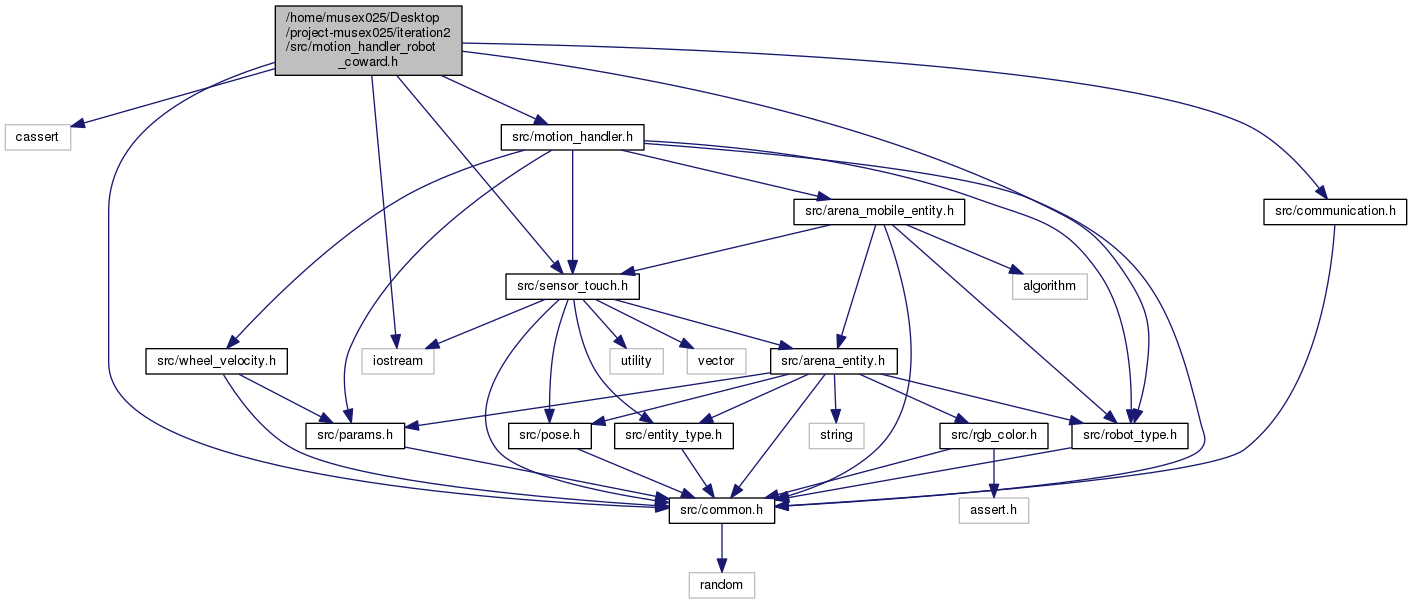
\includegraphics[width=350pt]{motion__handler__robot__coward_8h__incl}
\end{center}
\end{figure}
This graph shows which files directly or indirectly include this file\+:\nopagebreak
\begin{figure}[H]
\begin{center}
\leavevmode
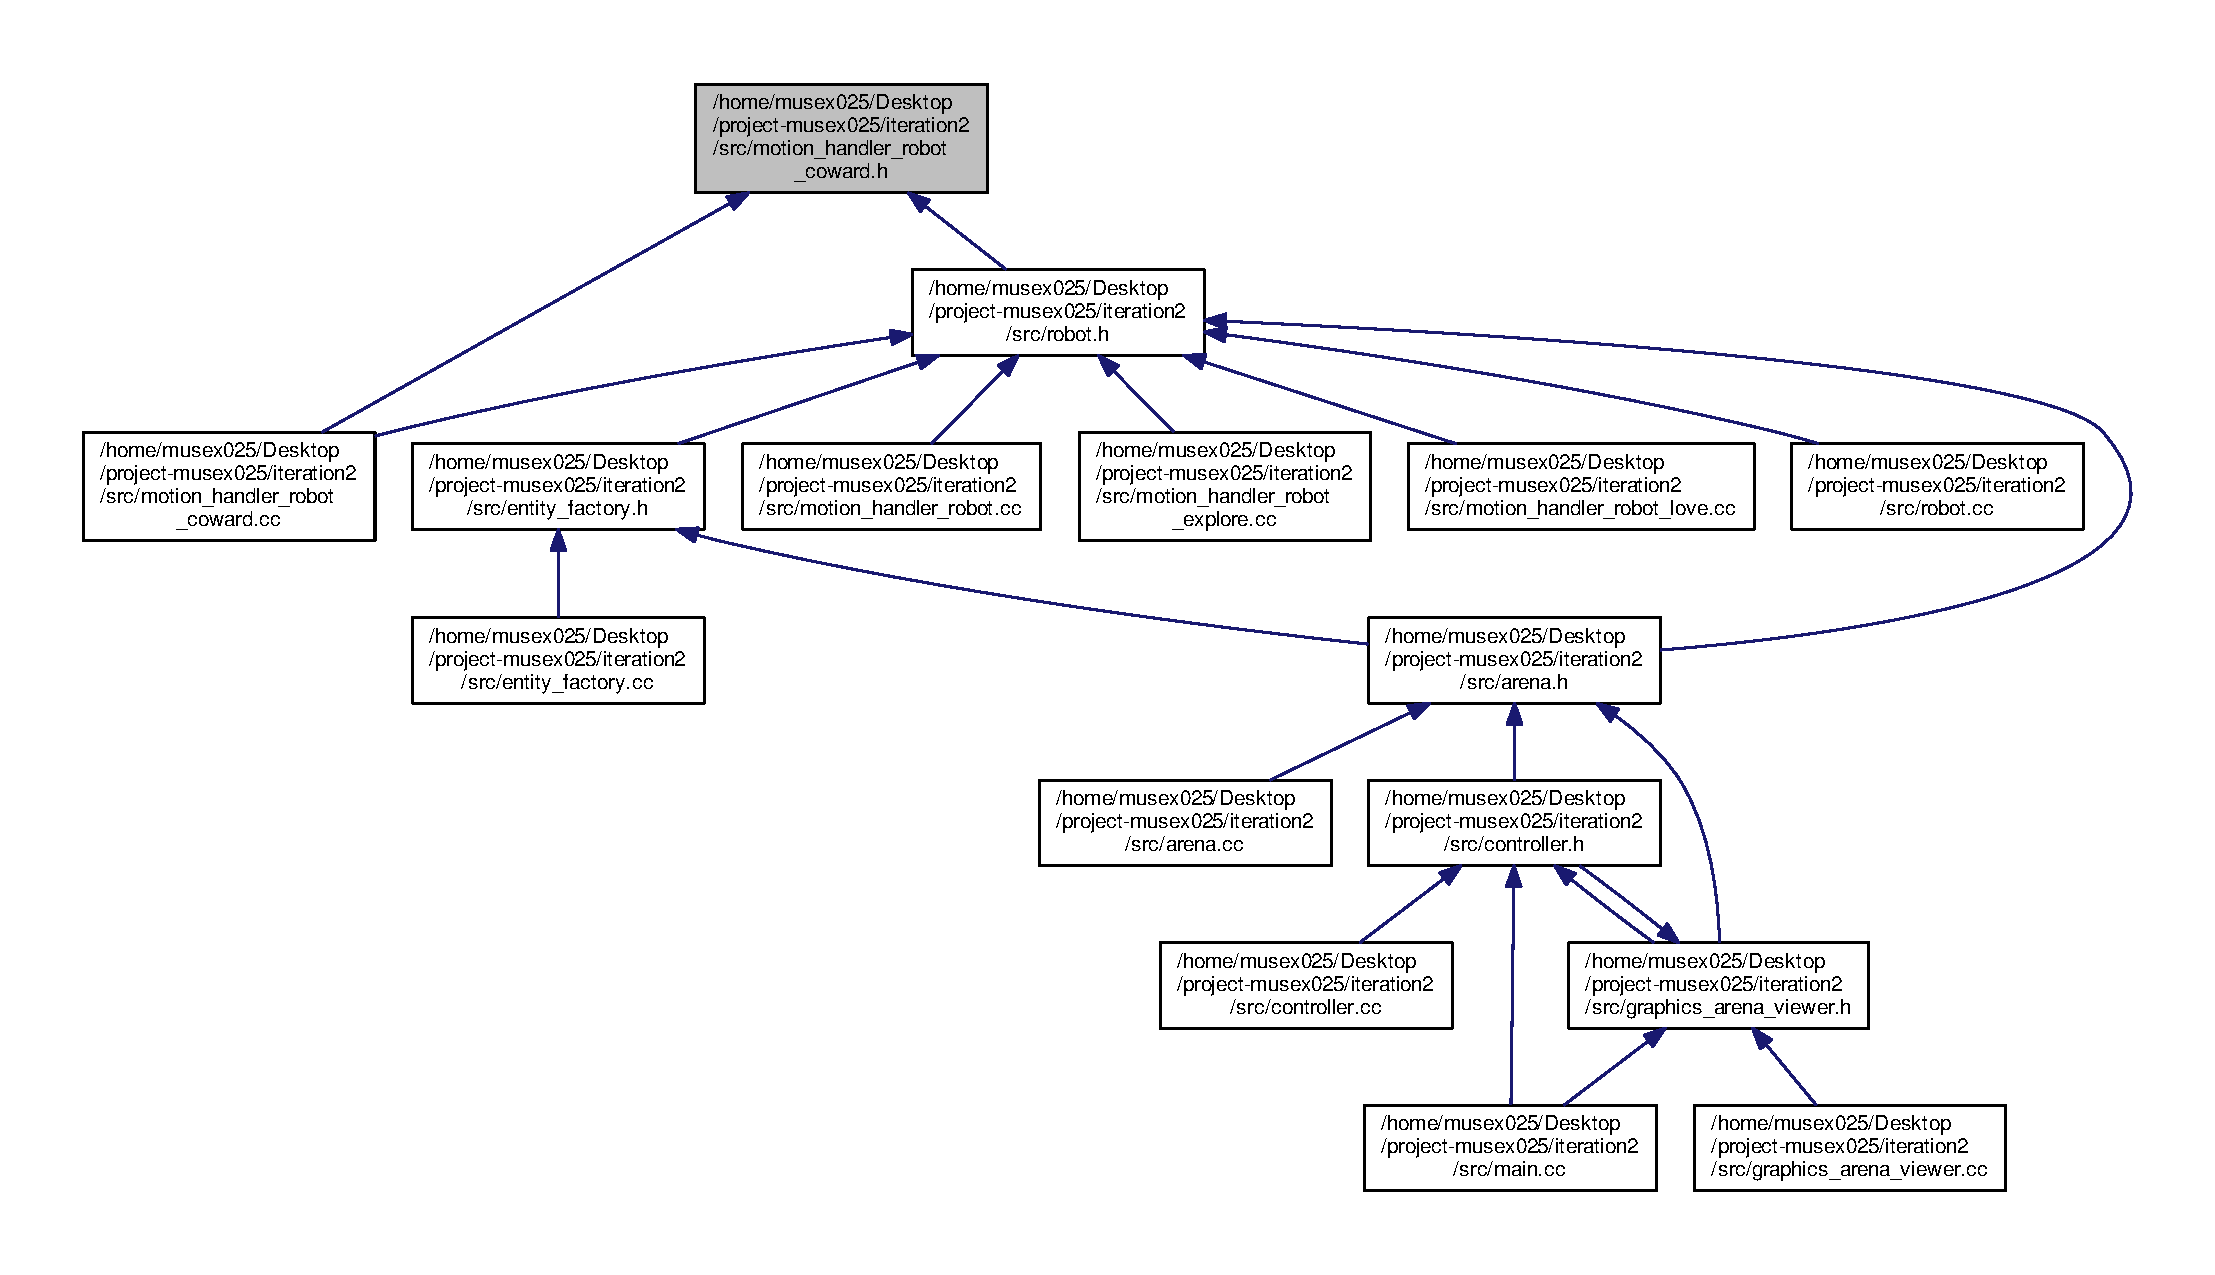
\includegraphics[width=350pt]{motion__handler__robot__coward_8h__dep__incl}
\end{center}
\end{figure}
\subsection*{Classes}
\begin{DoxyCompactItemize}
\item 
class \hyperlink{classMotionHandlerRobotCoward}{Motion\+Handler\+Robot\+Coward}
\begin{DoxyCompactList}\small\item\em Class managing a \hyperlink{classRobot}{Robot}\textquotesingle{}s and \hyperlink{classLight}{Light}\textquotesingle{}s speed and heading angle based on coward sesnor reading. \end{DoxyCompactList}\end{DoxyCompactItemize}
\subsection*{Functions}
\begin{DoxyCompactItemize}
\item 
{\bfseries N\+A\+M\+E\+S\+P\+A\+C\+E\+\_\+\+B\+E\+G\+IN} (csci3081)\hypertarget{motion__handler__robot__coward_8h_a5eaf22d0e7e2a0f12c6a660a6b011297}{}\label{motion__handler__robot__coward_8h_a5eaf22d0e7e2a0f12c6a660a6b011297}

\item 
{\bfseries N\+A\+M\+E\+S\+P\+A\+C\+E\+\_\+\+E\+ND} (csci3081)\hypertarget{motion__handler__robot__coward_8h_a0bc8eb973c3aef52acd7429898ace1cd}{}\label{motion__handler__robot__coward_8h_a0bc8eb973c3aef52acd7429898ace1cd}

\end{DoxyCompactItemize}


\subsection{Detailed Description}
\begin{DoxyCopyright}{Copyright}
2018 3081 Staff, All rights reserved. 
\end{DoxyCopyright}

\hypertarget{motion__handler__robot__explore_8cc}{}\section{src/motion\+\_\+handler\+\_\+robot\+\_\+explore.cc File Reference}
\label{motion__handler__robot__explore_8cc}\index{src/motion\+\_\+handler\+\_\+robot\+\_\+explore.\+cc@{src/motion\+\_\+handler\+\_\+robot\+\_\+explore.\+cc}}
{\ttfamily \#include \char`\"{}src/motion\+\_\+handler\+\_\+robot\+\_\+explore.\+h\char`\"{}}\\*
{\ttfamily \#include \char`\"{}src/motion\+\_\+behavior\+\_\+differential.\+h\char`\"{}}\\*
{\ttfamily \#include \char`\"{}src/robot.\+h\char`\"{}}\\*
{\ttfamily \#include \char`\"{}src/robot\+\_\+type.\+h\char`\"{}}\\*
\subsection*{Functions}
\begin{DoxyCompactItemize}
\item 
{\bfseries N\+A\+M\+E\+S\+P\+A\+C\+E\+\_\+\+B\+E\+G\+IN} (csci3081)\hypertarget{motion__handler__robot__explore_8cc_a5eaf22d0e7e2a0f12c6a660a6b011297}{}\label{motion__handler__robot__explore_8cc_a5eaf22d0e7e2a0f12c6a660a6b011297}

\item 
{\bfseries N\+A\+M\+E\+S\+P\+A\+C\+E\+\_\+\+E\+ND} (csci3081)\hypertarget{motion__handler__robot__explore_8cc_a0bc8eb973c3aef52acd7429898ace1cd}{}\label{motion__handler__robot__explore_8cc_a0bc8eb973c3aef52acd7429898ace1cd}

\end{DoxyCompactItemize}


\subsection{Detailed Description}
\begin{DoxyCopyright}{Copyright}
2018 3081 Staff, All rights reserved. 
\end{DoxyCopyright}

\hypertarget{motion__handler__robot__explore_8h}{}\section{src/motion\+\_\+handler\+\_\+robot\+\_\+explore.h File Reference}
\label{motion__handler__robot__explore_8h}\index{src/motion\+\_\+handler\+\_\+robot\+\_\+explore.\+h@{src/motion\+\_\+handler\+\_\+robot\+\_\+explore.\+h}}
{\ttfamily \#include $<$cassert$>$}\\*
{\ttfamily \#include $<$iostream$>$}\\*
{\ttfamily \#include \char`\"{}src/common.\+h\char`\"{}}\\*
{\ttfamily \#include \char`\"{}src/motion\+\_\+handler.\+h\char`\"{}}\\*
{\ttfamily \#include \char`\"{}src/sensor\+\_\+touch.\+h\char`\"{}}\\*
{\ttfamily \#include \char`\"{}src/communication.\+h\char`\"{}}\\*
{\ttfamily \#include \char`\"{}src/robot\+\_\+type.\+h\char`\"{}}\\*
\subsection*{Classes}
\begin{DoxyCompactItemize}
\item 
class \hyperlink{class_motion_handler_robot_explore}{Motion\+Handler\+Robot\+Explore}
\begin{DoxyCompactList}\small\item\em Class managing a \hyperlink{class_robot}{Robot}\textquotesingle{}s and \hyperlink{class_light}{Light}\textquotesingle{}s speed and heading angle based on the explore sensor readings. \end{DoxyCompactList}\end{DoxyCompactItemize}
\subsection*{Functions}
\begin{DoxyCompactItemize}
\item 
{\bfseries N\+A\+M\+E\+S\+P\+A\+C\+E\+\_\+\+B\+E\+G\+IN} (csci3081)\hypertarget{motion__handler__robot__explore_8h_a5eaf22d0e7e2a0f12c6a660a6b011297}{}\label{motion__handler__robot__explore_8h_a5eaf22d0e7e2a0f12c6a660a6b011297}

\item 
{\bfseries N\+A\+M\+E\+S\+P\+A\+C\+E\+\_\+\+E\+ND} (csci3081)\hypertarget{motion__handler__robot__explore_8h_a0bc8eb973c3aef52acd7429898ace1cd}{}\label{motion__handler__robot__explore_8h_a0bc8eb973c3aef52acd7429898ace1cd}

\end{DoxyCompactItemize}


\subsection{Detailed Description}
\begin{DoxyCopyright}{Copyright}
2018 3081 Staff, All rights reserved. 
\end{DoxyCopyright}

\hypertarget{motion__handler__robot__love_8cc}{}\section{src/motion\+\_\+handler\+\_\+robot\+\_\+love.cc File Reference}
\label{motion__handler__robot__love_8cc}\index{src/motion\+\_\+handler\+\_\+robot\+\_\+love.\+cc@{src/motion\+\_\+handler\+\_\+robot\+\_\+love.\+cc}}
{\ttfamily \#include \char`\"{}src/motion\+\_\+handler\+\_\+robot\+\_\+love.\+h\char`\"{}}\\*
{\ttfamily \#include \char`\"{}src/motion\+\_\+behavior\+\_\+differential.\+h\char`\"{}}\\*
{\ttfamily \#include \char`\"{}src/robot.\+h\char`\"{}}\\*
{\ttfamily \#include \char`\"{}src/robot\+\_\+type.\+h\char`\"{}}\\*
\subsection*{Functions}
\begin{DoxyCompactItemize}
\item 
{\bfseries N\+A\+M\+E\+S\+P\+A\+C\+E\+\_\+\+B\+E\+G\+IN} (csci3081)\hypertarget{motion__handler__robot__love_8cc_a5eaf22d0e7e2a0f12c6a660a6b011297}{}\label{motion__handler__robot__love_8cc_a5eaf22d0e7e2a0f12c6a660a6b011297}

\item 
{\bfseries N\+A\+M\+E\+S\+P\+A\+C\+E\+\_\+\+E\+ND} (csci3081)\hypertarget{motion__handler__robot__love_8cc_a0bc8eb973c3aef52acd7429898ace1cd}{}\label{motion__handler__robot__love_8cc_a0bc8eb973c3aef52acd7429898ace1cd}

\end{DoxyCompactItemize}


\subsection{Detailed Description}
\begin{DoxyCopyright}{Copyright}
2018 3081 Staff, All rights reserved. 
\end{DoxyCopyright}

\hypertarget{motion__handler__robot__love_8h}{}\section{src/motion\+\_\+handler\+\_\+robot\+\_\+love.h File Reference}
\label{motion__handler__robot__love_8h}\index{src/motion\+\_\+handler\+\_\+robot\+\_\+love.\+h@{src/motion\+\_\+handler\+\_\+robot\+\_\+love.\+h}}
{\ttfamily \#include $<$cassert$>$}\newline
{\ttfamily \#include $<$iostream$>$}\newline
{\ttfamily \#include \char`\"{}src/common.\+h\char`\"{}}\newline
{\ttfamily \#include \char`\"{}src/motion\+\_\+handler.\+h\char`\"{}}\newline
{\ttfamily \#include \char`\"{}src/sensor\+\_\+touch.\+h\char`\"{}}\newline
{\ttfamily \#include \char`\"{}src/communication.\+h\char`\"{}}\newline
{\ttfamily \#include \char`\"{}src/robot\+\_\+type.\+h\char`\"{}}\newline
\subsection*{Classes}
\begin{DoxyCompactItemize}
\item 
class \mbox{\hyperlink{class_motion_handler_robot_love}{Motion\+Handler\+Robot\+Love}}
\begin{DoxyCompactList}\small\item\em Class managing a \mbox{\hyperlink{class_robot}{Robot}}\textquotesingle{}s and \mbox{\hyperlink{class_light}{Light}}\textquotesingle{}s speed and heading angle based on the love sensor readings. \end{DoxyCompactList}\end{DoxyCompactItemize}
\subsection*{Functions}
\begin{DoxyCompactItemize}
\item 
\mbox{\Hypertarget{motion__handler__robot__love_8h_a5eaf22d0e7e2a0f12c6a660a6b011297}\label{motion__handler__robot__love_8h_a5eaf22d0e7e2a0f12c6a660a6b011297}} 
{\bfseries N\+A\+M\+E\+S\+P\+A\+C\+E\+\_\+\+B\+E\+G\+IN} (csci3081)
\item 
\mbox{\Hypertarget{motion__handler__robot__love_8h_a0bc8eb973c3aef52acd7429898ace1cd}\label{motion__handler__robot__love_8h_a0bc8eb973c3aef52acd7429898ace1cd}} 
{\bfseries N\+A\+M\+E\+S\+P\+A\+C\+E\+\_\+\+E\+ND} (csci3081)
\end{DoxyCompactItemize}


\subsection{Detailed Description}
\begin{DoxyCopyright}{Copyright}
2018 3081 Staff, All rights reserved. 
\end{DoxyCopyright}

\hypertarget{params_8h}{}\section{/home/musex025/\+Desktop/project-\/musex025/iteration2/src/params.h File Reference}
\label{params_8h}\index{/home/musex025/\+Desktop/project-\/musex025/iteration2/src/params.\+h@{/home/musex025/\+Desktop/project-\/musex025/iteration2/src/params.\+h}}
{\ttfamily \#include \char`\"{}src/common.\+h\char`\"{}}\\*
Include dependency graph for params.\+h\+:\nopagebreak
\begin{figure}[H]
\begin{center}
\leavevmode
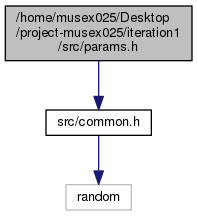
\includegraphics[width=220pt]{params_8h__incl}
\end{center}
\end{figure}
This graph shows which files directly or indirectly include this file\+:\nopagebreak
\begin{figure}[H]
\begin{center}
\leavevmode
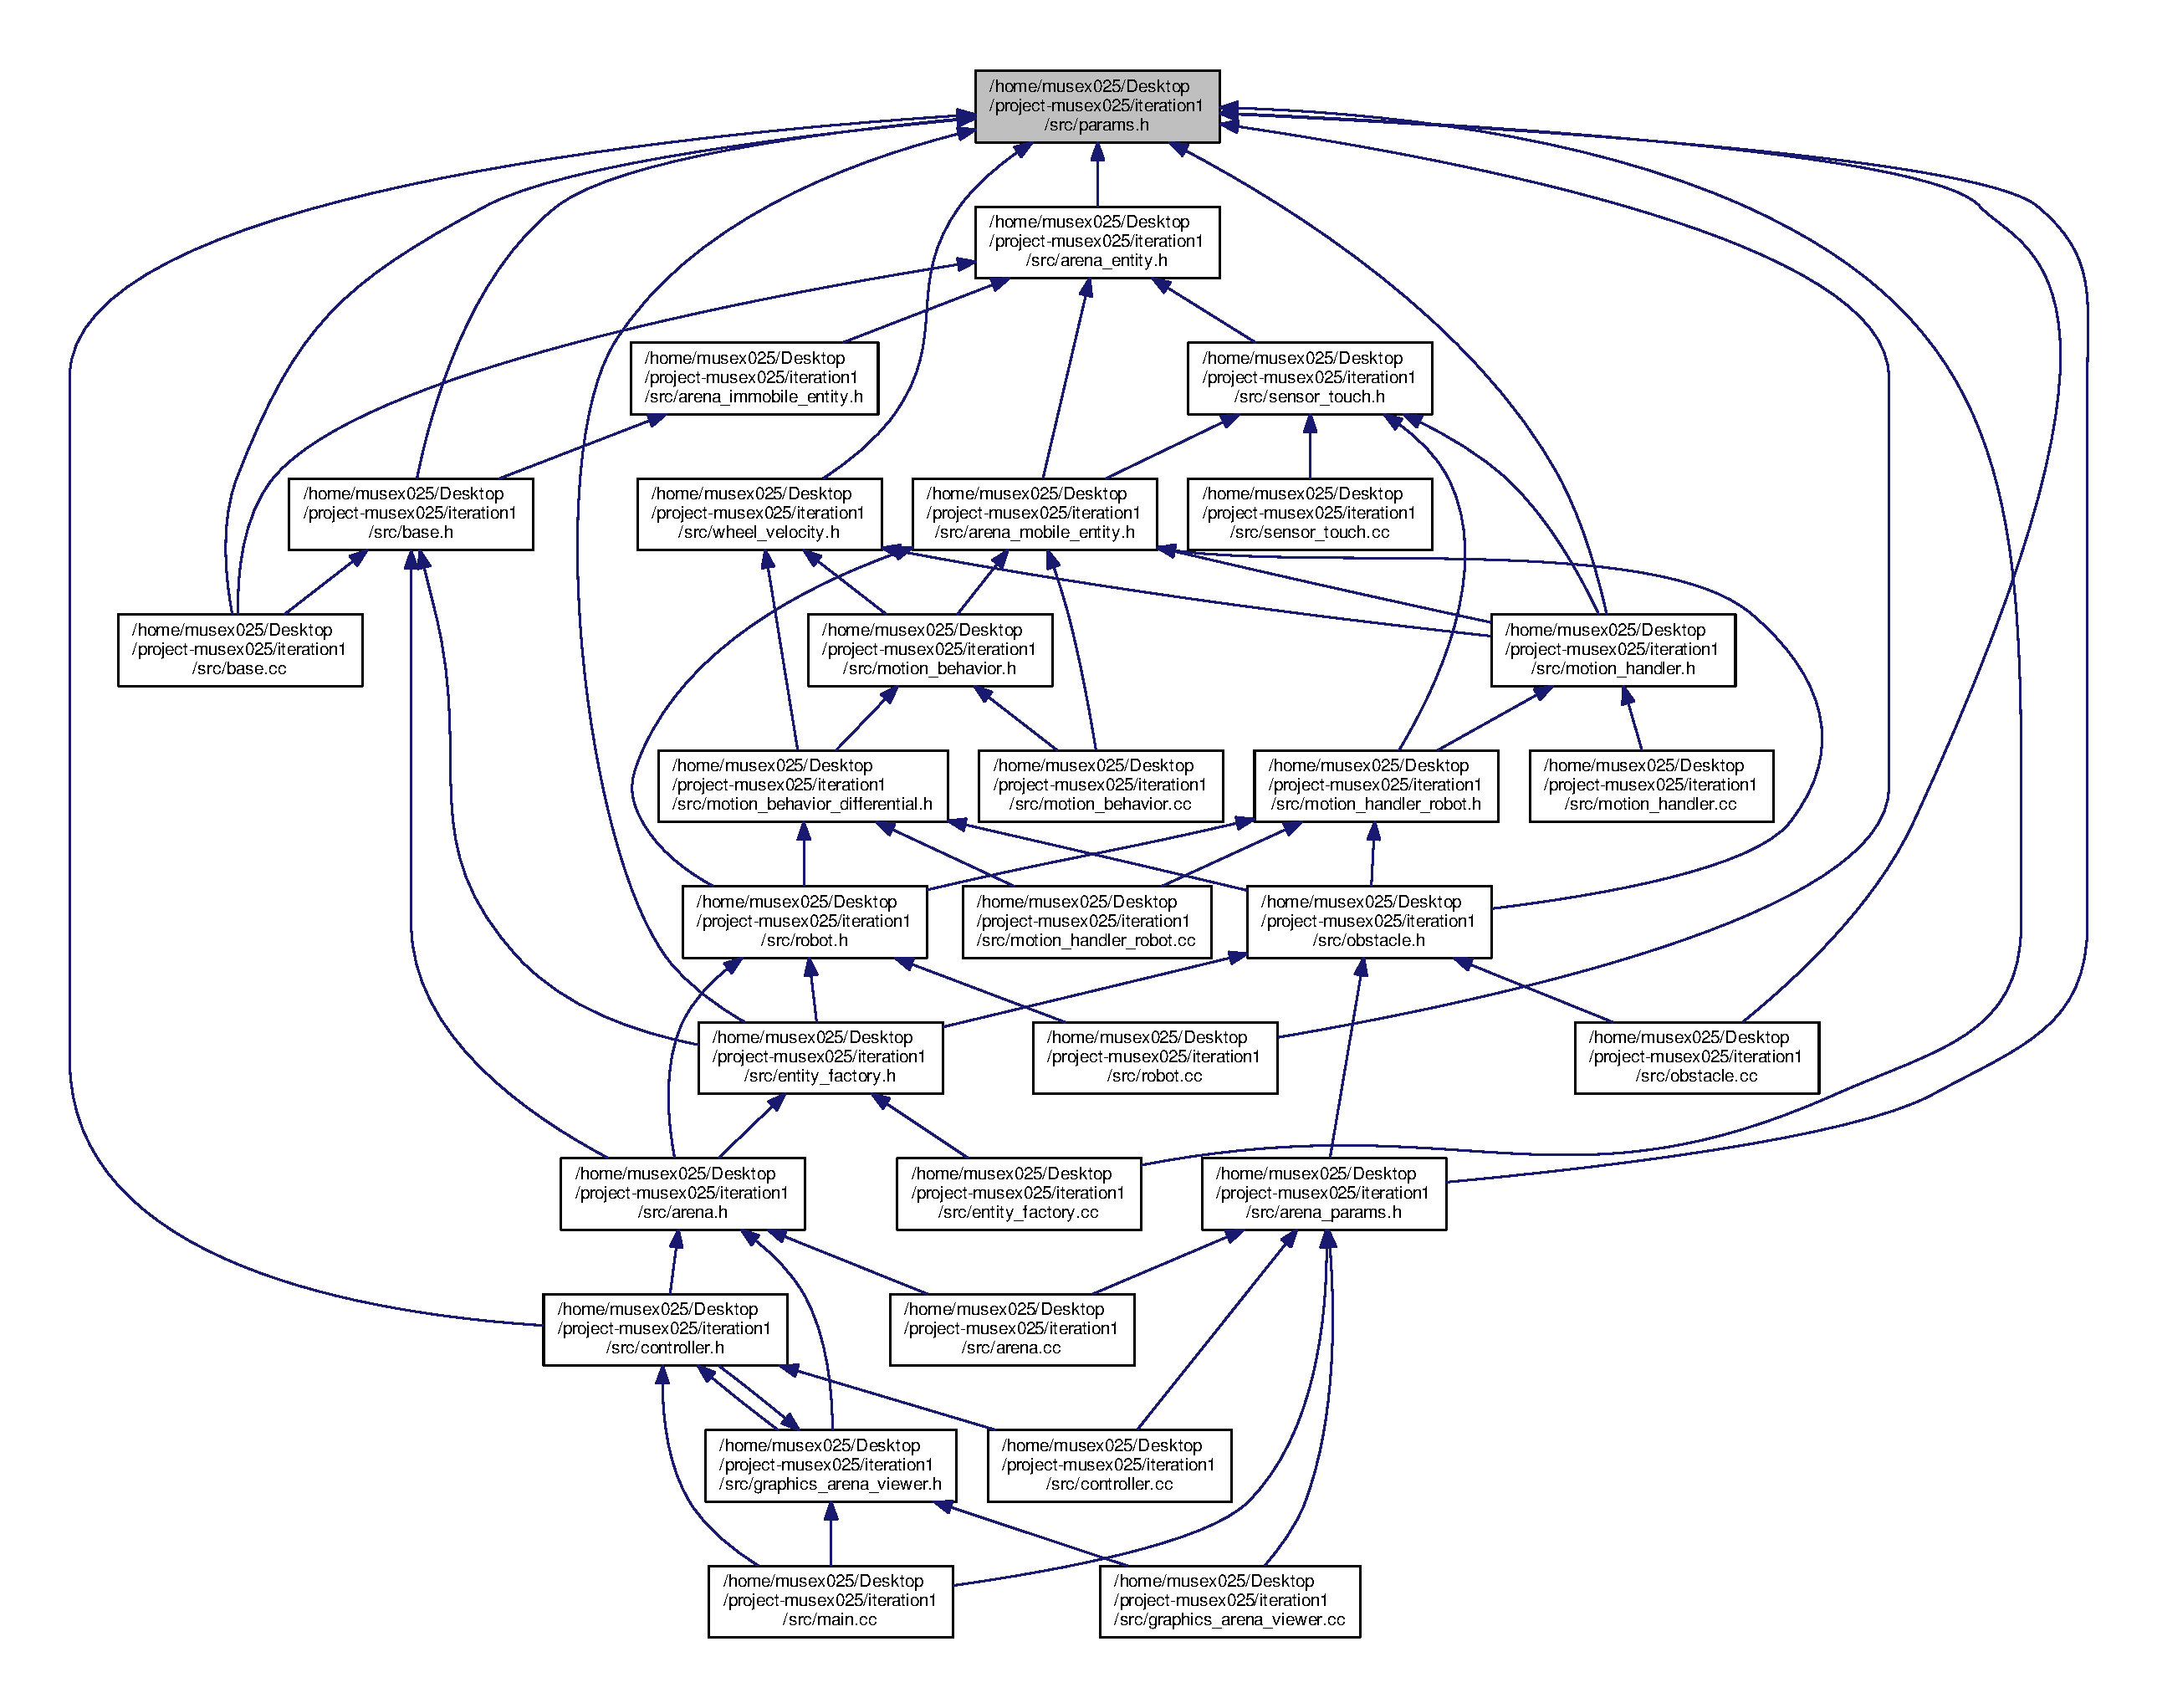
\includegraphics[width=350pt]{params_8h__dep__incl}
\end{center}
\end{figure}
\subsection*{Macros}
\begin{DoxyCompactItemize}
\item 
\#define {\bfseries X\+\_\+\+D\+IM}~1024\hypertarget{params_8h_a6a445f62f02793f2e8144b99e016cef9}{}\label{params_8h_a6a445f62f02793f2e8144b99e016cef9}

\item 
\#define {\bfseries Y\+\_\+\+D\+IM}~768\hypertarget{params_8h_a2cfec1e8b5f2afbb0211381d14376f22}{}\label{params_8h_a2cfec1e8b5f2afbb0211381d14376f22}

\item 
\#define {\bfseries T\+E\+X\+T\+\_\+\+B\+O\+X\+\_\+\+W\+I\+D\+TH}~50\hypertarget{params_8h_a8c8d7f7bde7f40b70c12ee765a49cac9}{}\label{params_8h_a8c8d7f7bde7f40b70c12ee765a49cac9}

\item 
\#define {\bfseries G\+U\+I\+\_\+\+M\+E\+N\+U\+\_\+\+W\+I\+D\+TH}~180\hypertarget{params_8h_add8b249b84443e0e5715c21c4916f433}{}\label{params_8h_add8b249b84443e0e5715c21c4916f433}

\item 
\#define {\bfseries G\+U\+I\+\_\+\+M\+E\+N\+U\+\_\+\+G\+AP}~10\hypertarget{params_8h_a5be4f0d679b1ad67f35b63c4e836aff0}{}\label{params_8h_a5be4f0d679b1ad67f35b63c4e836aff0}

\item 
\#define {\bfseries N\+\_\+\+LightS}~3\hypertarget{params_8h_ab3ff6777babb99ad91c03633807ab045}{}\label{params_8h_ab3ff6777babb99ad91c03633807ab045}

\item 
\#define {\bfseries M\+A\+X\+\_\+\+LightS}~8\hypertarget{params_8h_ab51d344a4987497f986ce6f194ed31b2}{}\label{params_8h_ab51d344a4987497f986ce6f194ed31b2}

\item 
\#define {\bfseries A\+R\+E\+N\+A\+\_\+\+X\+\_\+\+D\+IM}~X\+\_\+\+D\+IM\hypertarget{params_8h_ad88c43dbfe4f948310b09ec31cdb3904}{}\label{params_8h_ad88c43dbfe4f948310b09ec31cdb3904}

\item 
\#define {\bfseries A\+R\+E\+N\+A\+\_\+\+Y\+\_\+\+D\+IM}~Y\+\_\+\+D\+IM\hypertarget{params_8h_add1324fd92e8f2471d9415d4fc88e770}{}\label{params_8h_add1324fd92e8f2471d9415d4fc88e770}

\item 
\#define {\bfseries W\+ON}~0\hypertarget{params_8h_a0c78e81d71ff2b2f68b4904b83014269}{}\label{params_8h_a0c78e81d71ff2b2f68b4904b83014269}

\item 
\#define {\bfseries L\+O\+ST}~1\hypertarget{params_8h_a0d781d111f2907153eb8fd334b4495eb}{}\label{params_8h_a0d781d111f2907153eb8fd334b4495eb}

\item 
\#define {\bfseries P\+L\+A\+Y\+I\+NG}~2\hypertarget{params_8h_a1cab271d33d47905c89d4b7cbb84f505}{}\label{params_8h_a1cab271d33d47905c89d4b7cbb84f505}

\item 
\#define {\bfseries W\+O\+N\+\_\+\+C\+O\+L\+OR}~\{ 255, 0, 0 \}\hypertarget{params_8h_af527b88523bdd7301d1033c71b11f923}{}\label{params_8h_af527b88523bdd7301d1033c71b11f923}

\item 
\#define {\bfseries L\+O\+S\+S\+\_\+\+C\+O\+L\+OR}~\{ 75, 0, 150 \}\hypertarget{params_8h_a06929557523d9048aa08cc2f6c361020}{}\label{params_8h_a06929557523d9048aa08cc2f6c361020}

\item 
\#define {\bfseries D\+E\+F\+A\+U\+L\+T\+\_\+\+P\+O\+SE}~\{ 200, 200, 0\}\hypertarget{params_8h_a15c34f82cc34bbc409a6fe7319864d2d}{}\label{params_8h_a15c34f82cc34bbc409a6fe7319864d2d}

\item 
\#define {\bfseries D\+E\+F\+A\+U\+L\+T\+\_\+\+C\+O\+L\+OR}~\{ 255, 255, 255 \}\hypertarget{params_8h_a6218ebf3d38879af3e58f18e39c4e064}{}\label{params_8h_a6218ebf3d38879af3e58f18e39c4e064}

\item 
\#define {\bfseries D\+E\+F\+A\+U\+L\+T\+\_\+\+R\+A\+D\+I\+US}~20\hypertarget{params_8h_afd1ca313bdba9ff49bf0c988482d7bc5}{}\label{params_8h_afd1ca313bdba9ff49bf0c988482d7bc5}

\item 
\#define {\bfseries S\+T\+A\+R\+T\+I\+N\+G\+\_\+\+V\+E\+L\+O\+C\+I\+TY}~0.\+0\hypertarget{params_8h_a083f35ec458f711db575bea2cf9e4c41}{}\label{params_8h_a083f35ec458f711db575bea2cf9e4c41}

\item 
\#define {\bfseries R\+O\+B\+O\+T\+\_\+\+A\+N\+G\+L\+E\+\_\+\+D\+E\+L\+TA}~1\hypertarget{params_8h_a458f59648c762fd6d4192f542818dd0e}{}\label{params_8h_a458f59648c762fd6d4192f542818dd0e}

\item 
\#define {\bfseries R\+O\+B\+O\+T\+\_\+\+S\+P\+E\+E\+D\+\_\+\+D\+E\+L\+TA}~1\hypertarget{params_8h_a7313c284cdae0b1b8fa038a13d117abe}{}\label{params_8h_a7313c284cdae0b1b8fa038a13d117abe}

\item 
\#define {\bfseries R\+O\+B\+O\+T\+\_\+\+C\+O\+L\+L\+I\+S\+I\+O\+N\+\_\+\+D\+E\+L\+TA}~1\hypertarget{params_8h_a9806b15a37f6c861d403696c72228b35}{}\label{params_8h_a9806b15a37f6c861d403696c72228b35}

\item 
\#define {\bfseries R\+O\+B\+O\+T\+\_\+\+R\+A\+D\+I\+US}~16\hypertarget{params_8h_ab69dd643c61be536f4dc344cf7da0be6}{}\label{params_8h_ab69dd643c61be536f4dc344cf7da0be6}

\item 
\#define {\bfseries R\+O\+B\+O\+T\+\_\+\+I\+N\+I\+T\+\_\+\+P\+OS}~\{ 500, 500 , 0\}\hypertarget{params_8h_ad9027859aaee95122ea63b1ea5b92b1e}{}\label{params_8h_ad9027859aaee95122ea63b1ea5b92b1e}

\item 
\#define {\bfseries R\+O\+B\+O\+T\+\_\+\+C\+O\+L\+OR}~\{ 0, 0, 255 \}\hypertarget{params_8h_ac85c00b5d71e61a53461fc058be09917}{}\label{params_8h_ac85c00b5d71e61a53461fc058be09917}

\item 
\#define {\bfseries R\+O\+B\+O\+T\+\_\+\+H\+E\+A\+D\+I\+NG}~270\hypertarget{params_8h_a7e15e655a9975ed877928efb92648836}{}\label{params_8h_a7e15e655a9975ed877928efb92648836}

\item 
\#define {\bfseries R\+O\+B\+O\+T\+\_\+\+I\+N\+I\+T\+\_\+\+S\+P\+E\+ED}~0\hypertarget{params_8h_a52e3f00aa8a1318dd578630a2f338497}{}\label{params_8h_a52e3f00aa8a1318dd578630a2f338497}

\item 
\#define {\bfseries R\+O\+B\+O\+T\+\_\+\+M\+A\+X\+\_\+\+S\+P\+E\+ED}~10\hypertarget{params_8h_a4381547d29c949b82974be3f07ac6139}{}\label{params_8h_a4381547d29c949b82974be3f07ac6139}

\item 
\#define {\bfseries R\+O\+B\+O\+T\+\_\+\+M\+A\+X\+\_\+\+A\+N\+G\+LE}~360\hypertarget{params_8h_ad633036496d0df0464153fcf0fbffdd8}{}\label{params_8h_ad633036496d0df0464153fcf0fbffdd8}

\item 
\#define {\bfseries F\+O\+O\+D\+\_\+\+R\+A\+D\+I\+US}~20\hypertarget{params_8h_aa5506e14c6d016581e17a4fb9e51a8b5}{}\label{params_8h_aa5506e14c6d016581e17a4fb9e51a8b5}

\item 
\#define {\bfseries F\+O\+O\+D\+\_\+\+C\+O\+L\+L\+I\+S\+I\+O\+N\+\_\+\+D\+E\+L\+TA}~1\hypertarget{params_8h_a71b1151bdbf403c6133f72d156762f5b}{}\label{params_8h_a71b1151bdbf403c6133f72d156762f5b}

\item 
\#define {\bfseries F\+O\+O\+D\+\_\+\+I\+N\+I\+T\+\_\+\+P\+OS}~\{ 400, 400 \}\hypertarget{params_8h_a64c1ca26c932450e2d1e9a88598c657e}{}\label{params_8h_a64c1ca26c932450e2d1e9a88598c657e}

\item 
\#define {\bfseries F\+O\+O\+D\+\_\+\+C\+O\+L\+OR}~\{ 255, 0, 0 \}\hypertarget{params_8h_a397152d3f4b23cdfca1767996b6ff806}{}\label{params_8h_a397152d3f4b23cdfca1767996b6ff806}

\item 
\#define {\bfseries F\+O\+O\+D\+\_\+\+C\+O\+L\+O\+R\+\_\+\+P\+O\+S\+T\+\_\+\+C\+O\+L\+L\+I\+S\+I\+ON}~\{ 255, 255, 0 \}\hypertarget{params_8h_ab10440789ce925dbd306cb08bd732060}{}\label{params_8h_ab10440789ce925dbd306cb08bd732060}

\item 
\#define {\bfseries Light\+\_\+\+P\+O\+S\+I\+T\+I\+ON}~\{ 200, 200 \}\hypertarget{params_8h_aa4896cc0db3fb6803e91804659cc73fa}{}\label{params_8h_aa4896cc0db3fb6803e91804659cc73fa}

\item 
\#define {\bfseries Light\+\_\+\+R\+A\+D\+I\+US}~30\hypertarget{params_8h_a605c199fd3c9e3c05e3e309b8ed61300}{}\label{params_8h_a605c199fd3c9e3c05e3e309b8ed61300}

\item 
\#define {\bfseries Light\+\_\+\+M\+I\+N\+\_\+\+R\+A\+D\+I\+US}~10\hypertarget{params_8h_a6228189e23787dee760842d5eca0b76a}{}\label{params_8h_a6228189e23787dee760842d5eca0b76a}

\item 
\#define {\bfseries Light\+\_\+\+M\+A\+X\+\_\+\+R\+A\+D\+I\+US}~50\hypertarget{params_8h_a531d9257647c3a983cb4191517ea7e8e}{}\label{params_8h_a531d9257647c3a983cb4191517ea7e8e}

\item 
\#define {\bfseries Light\+\_\+\+C\+O\+L\+OR}~\{ 255, 255, 255 \}\hypertarget{params_8h_afeea5b7eff964967672ac0055427fb3b}{}\label{params_8h_afeea5b7eff964967672ac0055427fb3b}

\item 
\#define {\bfseries Light\+\_\+\+H\+E\+A\+D\+I\+NG}~270\hypertarget{params_8h_aea8683d252a83a0eb69cfa36c3b3033d}{}\label{params_8h_aea8683d252a83a0eb69cfa36c3b3033d}

\item 
\#define {\bfseries Light\+\_\+\+I\+N\+I\+T\+\_\+\+S\+P\+E\+ED}~0\hypertarget{params_8h_ac72d9ffa32c4379bc5a57402242de43a}{}\label{params_8h_ac72d9ffa32c4379bc5a57402242de43a}

\item 
\#define {\bfseries Light\+\_\+\+M\+A\+X\+\_\+\+S\+P\+E\+ED}~10\hypertarget{params_8h_a53b12814338d268f9aa016c94702cc9e}{}\label{params_8h_a53b12814338d268f9aa016c94702cc9e}

\item 
\#define {\bfseries Light\+\_\+\+M\+A\+X\+\_\+\+A\+N\+G\+LE}~360\hypertarget{params_8h_aa144d837ade10e1d87121761da476103}{}\label{params_8h_aa144d837ade10e1d87121761da476103}

\end{DoxyCompactItemize}


\subsection{Detailed Description}
\begin{DoxyCopyright}{Copyright}
2017 3081 Staff, All rights reserved. 
\end{DoxyCopyright}

\hypertarget{pose_8h}{}\section{src/pose.h File Reference}
\label{pose_8h}\index{src/pose.\+h@{src/pose.\+h}}
{\ttfamily \#include \char`\"{}src/common.\+h\char`\"{}}\newline
\subsection*{Classes}
\begin{DoxyCompactItemize}
\item 
struct \mbox{\hyperlink{struct_pose}{Pose}}
\begin{DoxyCompactList}\small\item\em A simple representation of the position/orientation of an entity within the \mbox{\hyperlink{class_arena}{Arena}}. \end{DoxyCompactList}\end{DoxyCompactItemize}
\subsection*{Functions}
\begin{DoxyCompactItemize}
\item 
\mbox{\Hypertarget{pose_8h_a5eaf22d0e7e2a0f12c6a660a6b011297}\label{pose_8h_a5eaf22d0e7e2a0f12c6a660a6b011297}} 
{\bfseries N\+A\+M\+E\+S\+P\+A\+C\+E\+\_\+\+B\+E\+G\+IN} (csci3081)
\item 
\mbox{\Hypertarget{pose_8h_a8ff75d4ff876fdefe002a43215eb0511}\label{pose_8h_a8ff75d4ff876fdefe002a43215eb0511}} 
constexpr double {\bfseries deg2rad} (double deg)
\item 
\mbox{\Hypertarget{pose_8h_a4c120723c2a7beeed4d1f0b9ee828a56}\label{pose_8h_a4c120723c2a7beeed4d1f0b9ee828a56}} 
constexpr double {\bfseries rad2deg} (double rad)
\item 
\mbox{\Hypertarget{pose_8h_a0bc8eb973c3aef52acd7429898ace1cd}\label{pose_8h_a0bc8eb973c3aef52acd7429898ace1cd}} 
{\bfseries N\+A\+M\+E\+S\+P\+A\+C\+E\+\_\+\+E\+ND} (csci3081)
\end{DoxyCompactItemize}


\subsection{Detailed Description}
\begin{DoxyCopyright}{Copyright}
2017 3081 Staff, All rights reserved. 
\end{DoxyCopyright}

\hypertarget{rgb__color_8cc}{}\section{/home/musex025/\+Desktop/project-\/musex025/iteration2/src/rgb\+\_\+color.cc File Reference}
\label{rgb__color_8cc}\index{/home/musex025/\+Desktop/project-\/musex025/iteration2/src/rgb\+\_\+color.\+cc@{/home/musex025/\+Desktop/project-\/musex025/iteration2/src/rgb\+\_\+color.\+cc}}
{\ttfamily \#include \char`\"{}src/rgb\+\_\+color.\+h\char`\"{}}\\*
Include dependency graph for rgb\+\_\+color.\+cc\+:\nopagebreak
\begin{figure}[H]
\begin{center}
\leavevmode
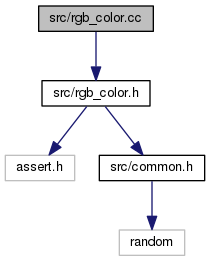
\includegraphics[width=232pt]{rgb__color_8cc__incl}
\end{center}
\end{figure}
\subsection*{Functions}
\begin{DoxyCompactItemize}
\item 
{\bfseries N\+A\+M\+E\+S\+P\+A\+C\+E\+\_\+\+B\+E\+G\+IN} (csci3081)\hypertarget{rgb__color_8cc_a5eaf22d0e7e2a0f12c6a660a6b011297}{}\label{rgb__color_8cc_a5eaf22d0e7e2a0f12c6a660a6b011297}

\item 
{\bfseries N\+A\+M\+E\+S\+P\+A\+C\+E\+\_\+\+E\+ND} (csci3081)\hypertarget{rgb__color_8cc_a0bc8eb973c3aef52acd7429898ace1cd}{}\label{rgb__color_8cc_a0bc8eb973c3aef52acd7429898ace1cd}

\end{DoxyCompactItemize}


\subsection{Detailed Description}
\begin{DoxyCopyright}{Copyright}
2018 3081 Staff, All rights reserved. 
\end{DoxyCopyright}

\hypertarget{rgb__color_8h}{}\section{src/rgb\+\_\+color.h File Reference}
\label{rgb__color_8h}\index{src/rgb\+\_\+color.\+h@{src/rgb\+\_\+color.\+h}}
{\ttfamily \#include $<$assert.\+h$>$}\newline
{\ttfamily \#include \char`\"{}src/common.\+h\char`\"{}}\newline
\subsection*{Classes}
\begin{DoxyCompactItemize}
\item 
struct \mbox{\hyperlink{struct_rgb_color}{Rgb\+Color}}
\begin{DoxyCompactList}\small\item\em Struct representing a rgb\+\_\+color. \end{DoxyCompactList}\end{DoxyCompactItemize}
\subsection*{Enumerations}
\begin{DoxyCompactItemize}
\item 
\mbox{\Hypertarget{rgb__color_8h_a00239091fc10bcecc92431d3fdb4e5c9}\label{rgb__color_8h_a00239091fc10bcecc92431d3fdb4e5c9}} 
enum {\bfseries Rgb\+Color\+Enum} \{ \newline
{\bfseries k\+Red}, 
{\bfseries k\+Green}, 
{\bfseries k\+Blue}, 
{\bfseries k\+Yellow}, 
\newline
{\bfseries k\+Orange}, 
{\bfseries k\+Purple}, 
{\bfseries k\+White}, 
{\bfseries k\+Black}
 \}
\end{DoxyCompactItemize}
\subsection*{Functions}
\begin{DoxyCompactItemize}
\item 
\mbox{\Hypertarget{rgb__color_8h_a5eaf22d0e7e2a0f12c6a660a6b011297}\label{rgb__color_8h_a5eaf22d0e7e2a0f12c6a660a6b011297}} 
{\bfseries N\+A\+M\+E\+S\+P\+A\+C\+E\+\_\+\+B\+E\+G\+IN} (csci3081)
\item 
\mbox{\Hypertarget{rgb__color_8h_a0bc8eb973c3aef52acd7429898ace1cd}\label{rgb__color_8h_a0bc8eb973c3aef52acd7429898ace1cd}} 
{\bfseries N\+A\+M\+E\+S\+P\+A\+C\+E\+\_\+\+E\+ND} (csci3081)
\end{DoxyCompactItemize}


\subsection{Detailed Description}
\begin{DoxyCopyright}{Copyright}
2017 3081 Staff, All rights reserved. 
\end{DoxyCopyright}

\hypertarget{robot_8cc}{}\section{src/robot.cc File Reference}
\label{robot_8cc}\index{src/robot.\+cc@{src/robot.\+cc}}
{\ttfamily \#include $<$cmath$>$}\\*
{\ttfamily \#include \char`\"{}src/robot.\+h\char`\"{}}\\*
{\ttfamily \#include \char`\"{}src/params.\+h\char`\"{}}\\*
{\ttfamily \#include \char`\"{}src/robot\+\_\+type.\+h\char`\"{}}\\*
\subsection*{Functions}
\begin{DoxyCompactItemize}
\item 
{\bfseries N\+A\+M\+E\+S\+P\+A\+C\+E\+\_\+\+B\+E\+G\+IN} (csci3081)\hypertarget{robot_8cc_a5eaf22d0e7e2a0f12c6a660a6b011297}{}\label{robot_8cc_a5eaf22d0e7e2a0f12c6a660a6b011297}

\item 
{\bfseries N\+A\+M\+E\+S\+P\+A\+C\+E\+\_\+\+E\+ND} (csci3081)\hypertarget{robot_8cc_a0bc8eb973c3aef52acd7429898ace1cd}{}\label{robot_8cc_a0bc8eb973c3aef52acd7429898ace1cd}

\end{DoxyCompactItemize}


\subsection{Detailed Description}
\begin{DoxyCopyright}{Copyright}
2017 3081 Staff, All rights reserved. 
\end{DoxyCopyright}

\hypertarget{robot_8h}{}\section{/home/musex025/\+Desktop/project-\/musex025/iteration1/src/robot.h File Reference}
\label{robot_8h}\index{/home/musex025/\+Desktop/project-\/musex025/iteration1/src/robot.\+h@{/home/musex025/\+Desktop/project-\/musex025/iteration1/src/robot.\+h}}
{\ttfamily \#include $<$string$>$}\\*
{\ttfamily \#include \char`\"{}src/arena\+\_\+mobile\+\_\+entity.\+h\char`\"{}}\\*
{\ttfamily \#include \char`\"{}src/common.\+h\char`\"{}}\\*
{\ttfamily \#include \char`\"{}src/motion\+\_\+handler\+\_\+robot.\+h\char`\"{}}\\*
{\ttfamily \#include \char`\"{}src/motion\+\_\+behavior\+\_\+differential.\+h\char`\"{}}\\*
{\ttfamily \#include \char`\"{}src/entity\+\_\+type.\+h\char`\"{}}\\*
Include dependency graph for robot.\+h\+:
\nopagebreak
\begin{figure}[H]
\begin{center}
\leavevmode
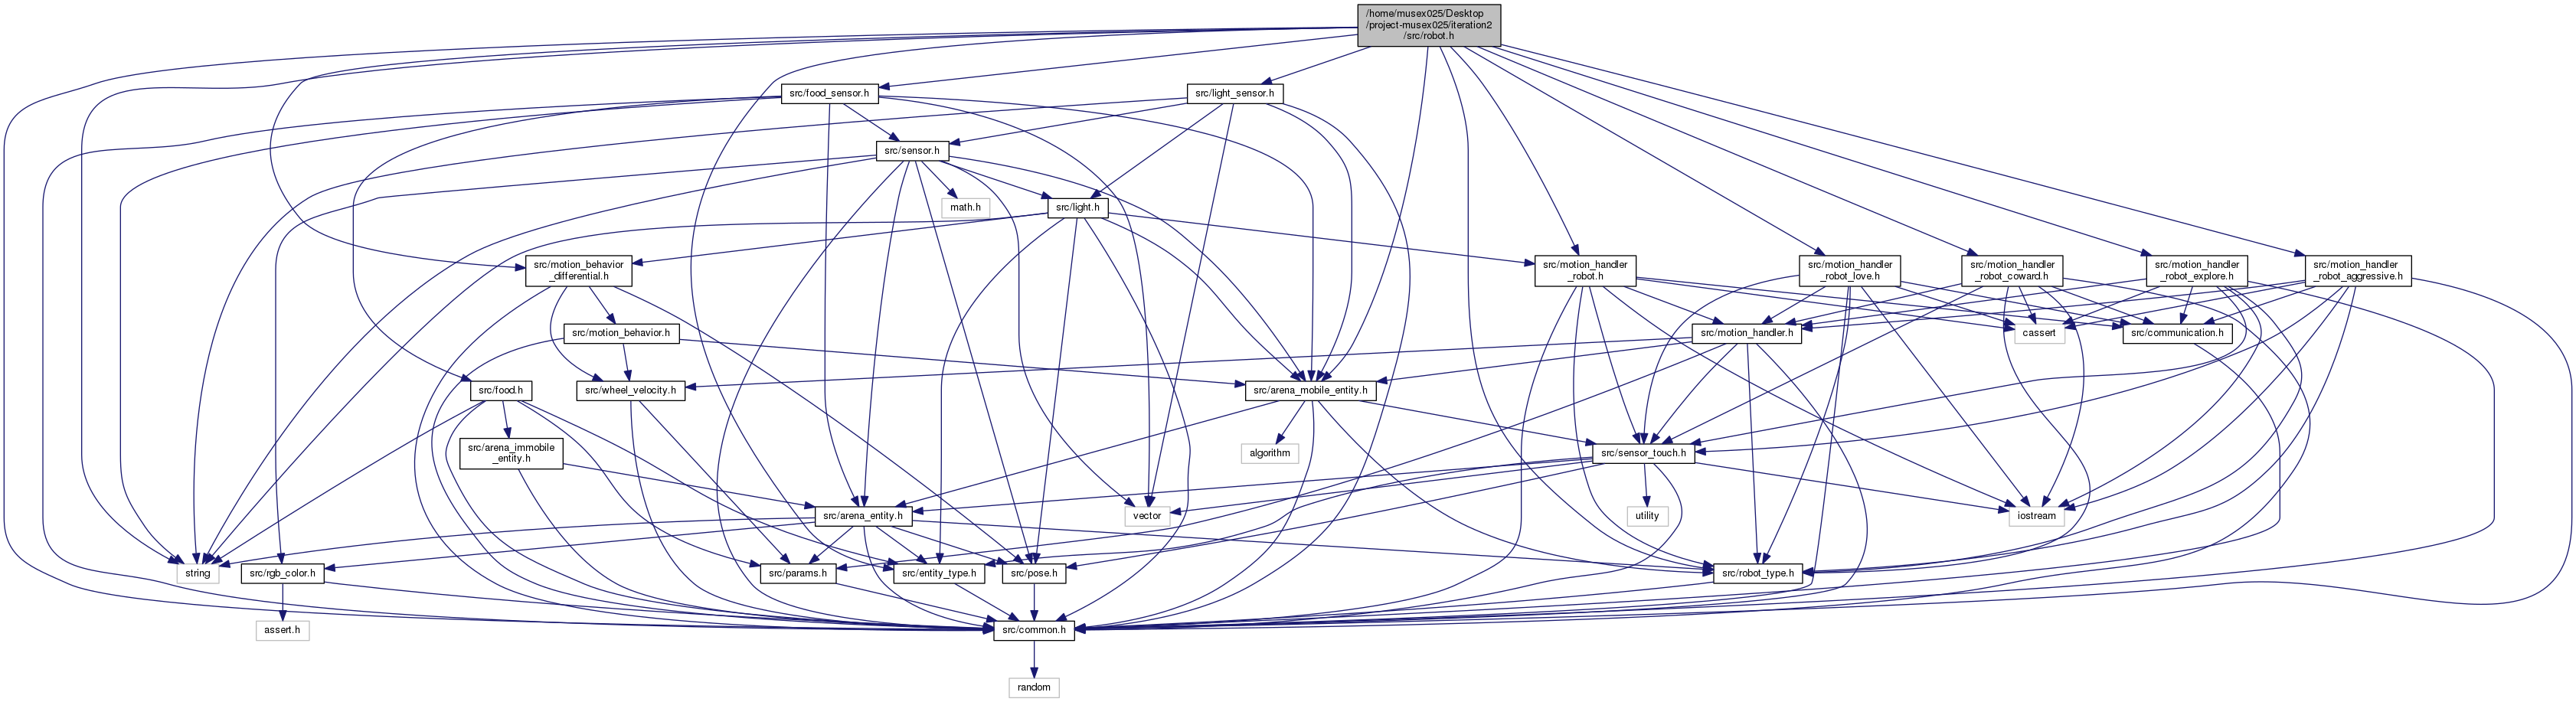
\includegraphics[width=350pt]{robot_8h__incl}
\end{center}
\end{figure}
This graph shows which files directly or indirectly include this file\+:
\nopagebreak
\begin{figure}[H]
\begin{center}
\leavevmode
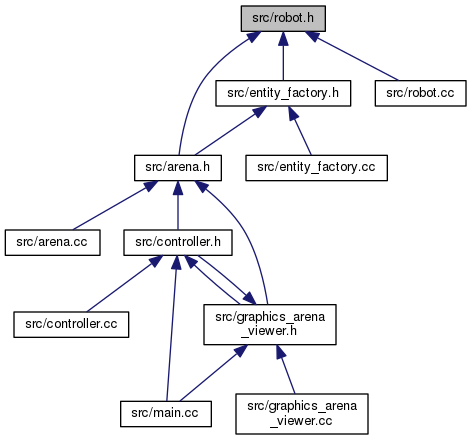
\includegraphics[width=350pt]{robot_8h__dep__incl}
\end{center}
\end{figure}
\subsection*{Classes}
\begin{DoxyCompactItemize}
\item 
class \hyperlink{classRobot}{Robot}
\begin{DoxyCompactList}\small\item\em Class representing a robot within the arena. \end{DoxyCompactList}\end{DoxyCompactItemize}
\subsection*{Functions}
\begin{DoxyCompactItemize}
\item 
{\bfseries N\+A\+M\+E\+S\+P\+A\+C\+E\+\_\+\+B\+E\+G\+IN} (csci3081)\hypertarget{robot_8h_a5eaf22d0e7e2a0f12c6a660a6b011297}{}\label{robot_8h_a5eaf22d0e7e2a0f12c6a660a6b011297}

\item 
{\bfseries N\+A\+M\+E\+S\+P\+A\+C\+E\+\_\+\+E\+ND} (csci3081)\hypertarget{robot_8h_a0bc8eb973c3aef52acd7429898ace1cd}{}\label{robot_8h_a0bc8eb973c3aef52acd7429898ace1cd}

\end{DoxyCompactItemize}


\subsection{Detailed Description}
\begin{DoxyCopyright}{Copyright}
2017 3081 Staff, All rights reserved. 
\end{DoxyCopyright}

\hypertarget{robot__type_8h}{}\section{src/robot\+\_\+type.h File Reference}
\label{robot__type_8h}\index{src/robot\+\_\+type.\+h@{src/robot\+\_\+type.\+h}}
{\ttfamily \#include \char`\"{}src/common.\+h\char`\"{}}\\*
\subsection*{Enumerations}
\begin{DoxyCompactItemize}
\item 
enum {\bfseries Robot\+Type} \{ \\*
{\bfseries k\+Love}, 
{\bfseries k\+Explore}, 
{\bfseries k\+Aggressive}, 
{\bfseries k\+Coward}, 
\\*
{\bfseries k\+Undefined\+RT}
 \}\hypertarget{robot__type_8h_a78d284d08fd22d809fd436256f2cbc39}{}\label{robot__type_8h_a78d284d08fd22d809fd436256f2cbc39}

\end{DoxyCompactItemize}
\subsection*{Functions}
\begin{DoxyCompactItemize}
\item 
{\bfseries N\+A\+M\+E\+S\+P\+A\+C\+E\+\_\+\+B\+E\+G\+IN} (csci3081)\hypertarget{robot__type_8h_a5eaf22d0e7e2a0f12c6a660a6b011297}{}\label{robot__type_8h_a5eaf22d0e7e2a0f12c6a660a6b011297}

\item 
{\bfseries N\+A\+M\+E\+S\+P\+A\+C\+E\+\_\+\+E\+ND} (csci3081)\hypertarget{robot__type_8h_a0bc8eb973c3aef52acd7429898ace1cd}{}\label{robot__type_8h_a0bc8eb973c3aef52acd7429898ace1cd}

\end{DoxyCompactItemize}


\subsection{Detailed Description}
\begin{DoxyCopyright}{Copyright}
2017 3081 Staff, All rights reserved. 
\end{DoxyCopyright}

\hypertarget{sensor_8cc}{}\section{/home/musex025/\+Desktop/project-\/musex025/iteration2/src/sensor.cc File Reference}
\label{sensor_8cc}\index{/home/musex025/\+Desktop/project-\/musex025/iteration2/src/sensor.\+cc@{/home/musex025/\+Desktop/project-\/musex025/iteration2/src/sensor.\+cc}}
{\ttfamily \#include \char`\"{}src/sensor.\+h\char`\"{}}\\*
{\ttfamily \#include $<$iostream$>$}\\*
Include dependency graph for sensor.\+cc\+:\nopagebreak
\begin{figure}[H]
\begin{center}
\leavevmode
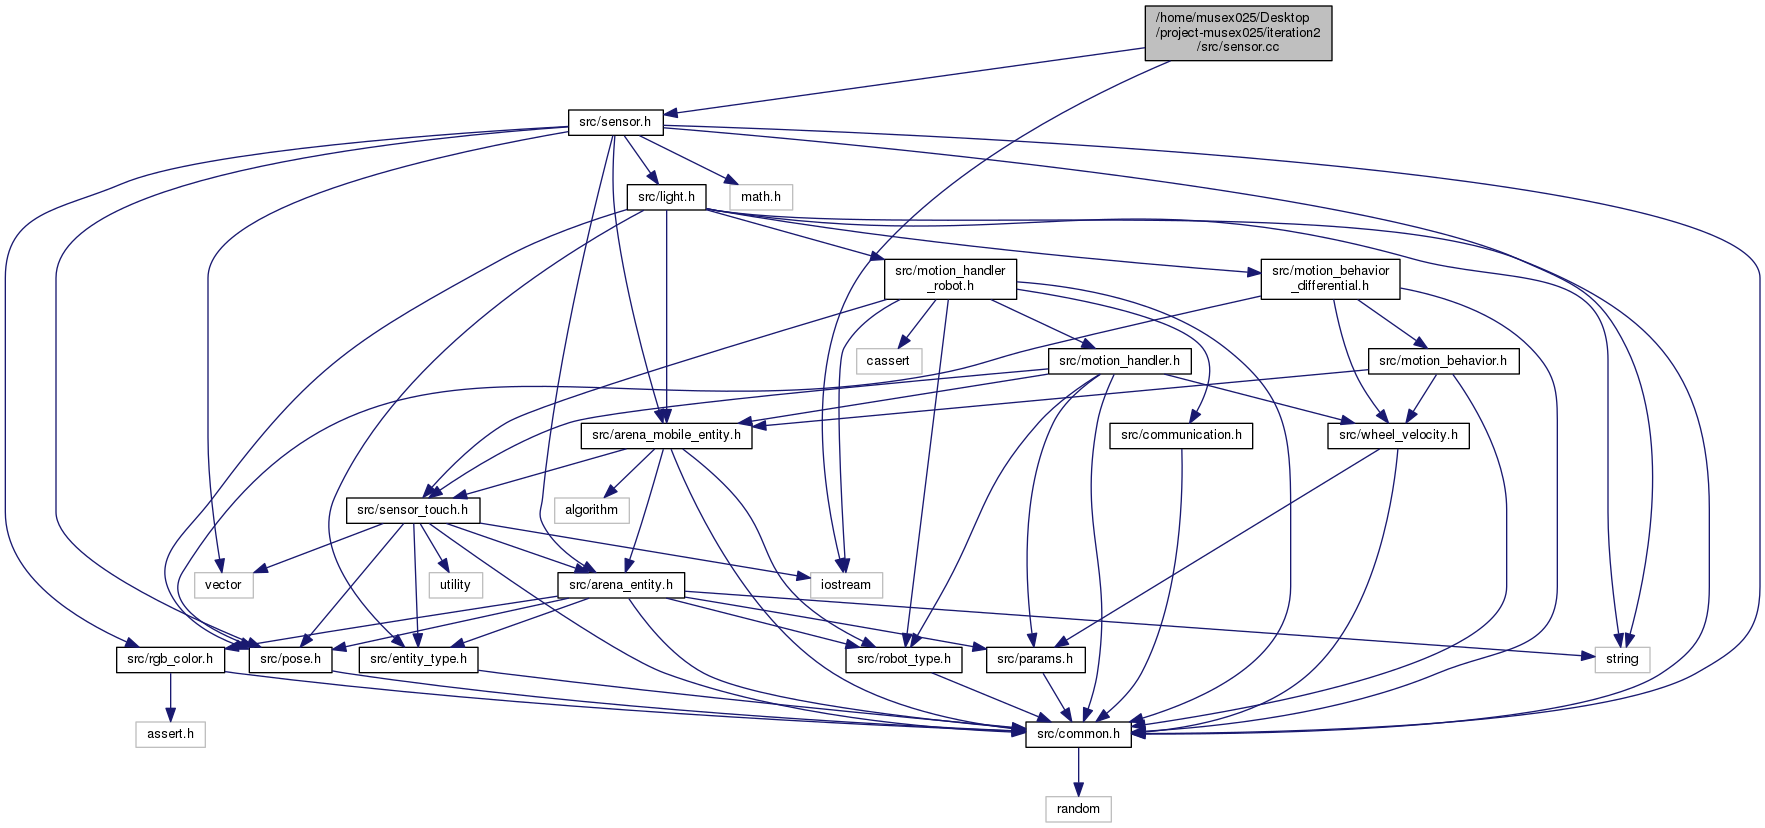
\includegraphics[width=350pt]{sensor_8cc__incl}
\end{center}
\end{figure}
\subsection*{Functions}
\begin{DoxyCompactItemize}
\item 
{\bfseries N\+A\+M\+E\+S\+P\+A\+C\+E\+\_\+\+B\+E\+G\+IN} (csci3081)\hypertarget{sensor_8cc_a5eaf22d0e7e2a0f12c6a660a6b011297}{}\label{sensor_8cc_a5eaf22d0e7e2a0f12c6a660a6b011297}

\item 
{\bfseries N\+A\+M\+E\+S\+P\+A\+C\+E\+\_\+\+E\+ND} (csci3081)\hypertarget{sensor_8cc_a0bc8eb973c3aef52acd7429898ace1cd}{}\label{sensor_8cc_a0bc8eb973c3aef52acd7429898ace1cd}

\end{DoxyCompactItemize}


\subsection{Detailed Description}
\begin{DoxyCopyright}{Copyright}
2017 3081 Staff, All rights reserved. 
\end{DoxyCopyright}

\hypertarget{sensor_8h}{}\section{/home/musex025/\+Desktop/project-\/musex025/iteration2/src/sensor.h File Reference}
\label{sensor_8h}\index{/home/musex025/\+Desktop/project-\/musex025/iteration2/src/sensor.\+h@{/home/musex025/\+Desktop/project-\/musex025/iteration2/src/sensor.\+h}}
{\ttfamily \#include $<$math.\+h$>$}\\*
{\ttfamily \#include $<$string$>$}\\*
{\ttfamily \#include $<$vector$>$}\\*
{\ttfamily \#include \char`\"{}src/common.\+h\char`\"{}}\\*
{\ttfamily \#include \char`\"{}src/pose.\+h\char`\"{}}\\*
{\ttfamily \#include \char`\"{}src/arena\+\_\+entity.\+h\char`\"{}}\\*
{\ttfamily \#include \char`\"{}src/rgb\+\_\+color.\+h\char`\"{}}\\*
{\ttfamily \#include \char`\"{}src/arena\+\_\+mobile\+\_\+entity.\+h\char`\"{}}\\*
{\ttfamily \#include \char`\"{}src/light.\+h\char`\"{}}\\*
Include dependency graph for sensor.\+h\+:\nopagebreak
\begin{figure}[H]
\begin{center}
\leavevmode
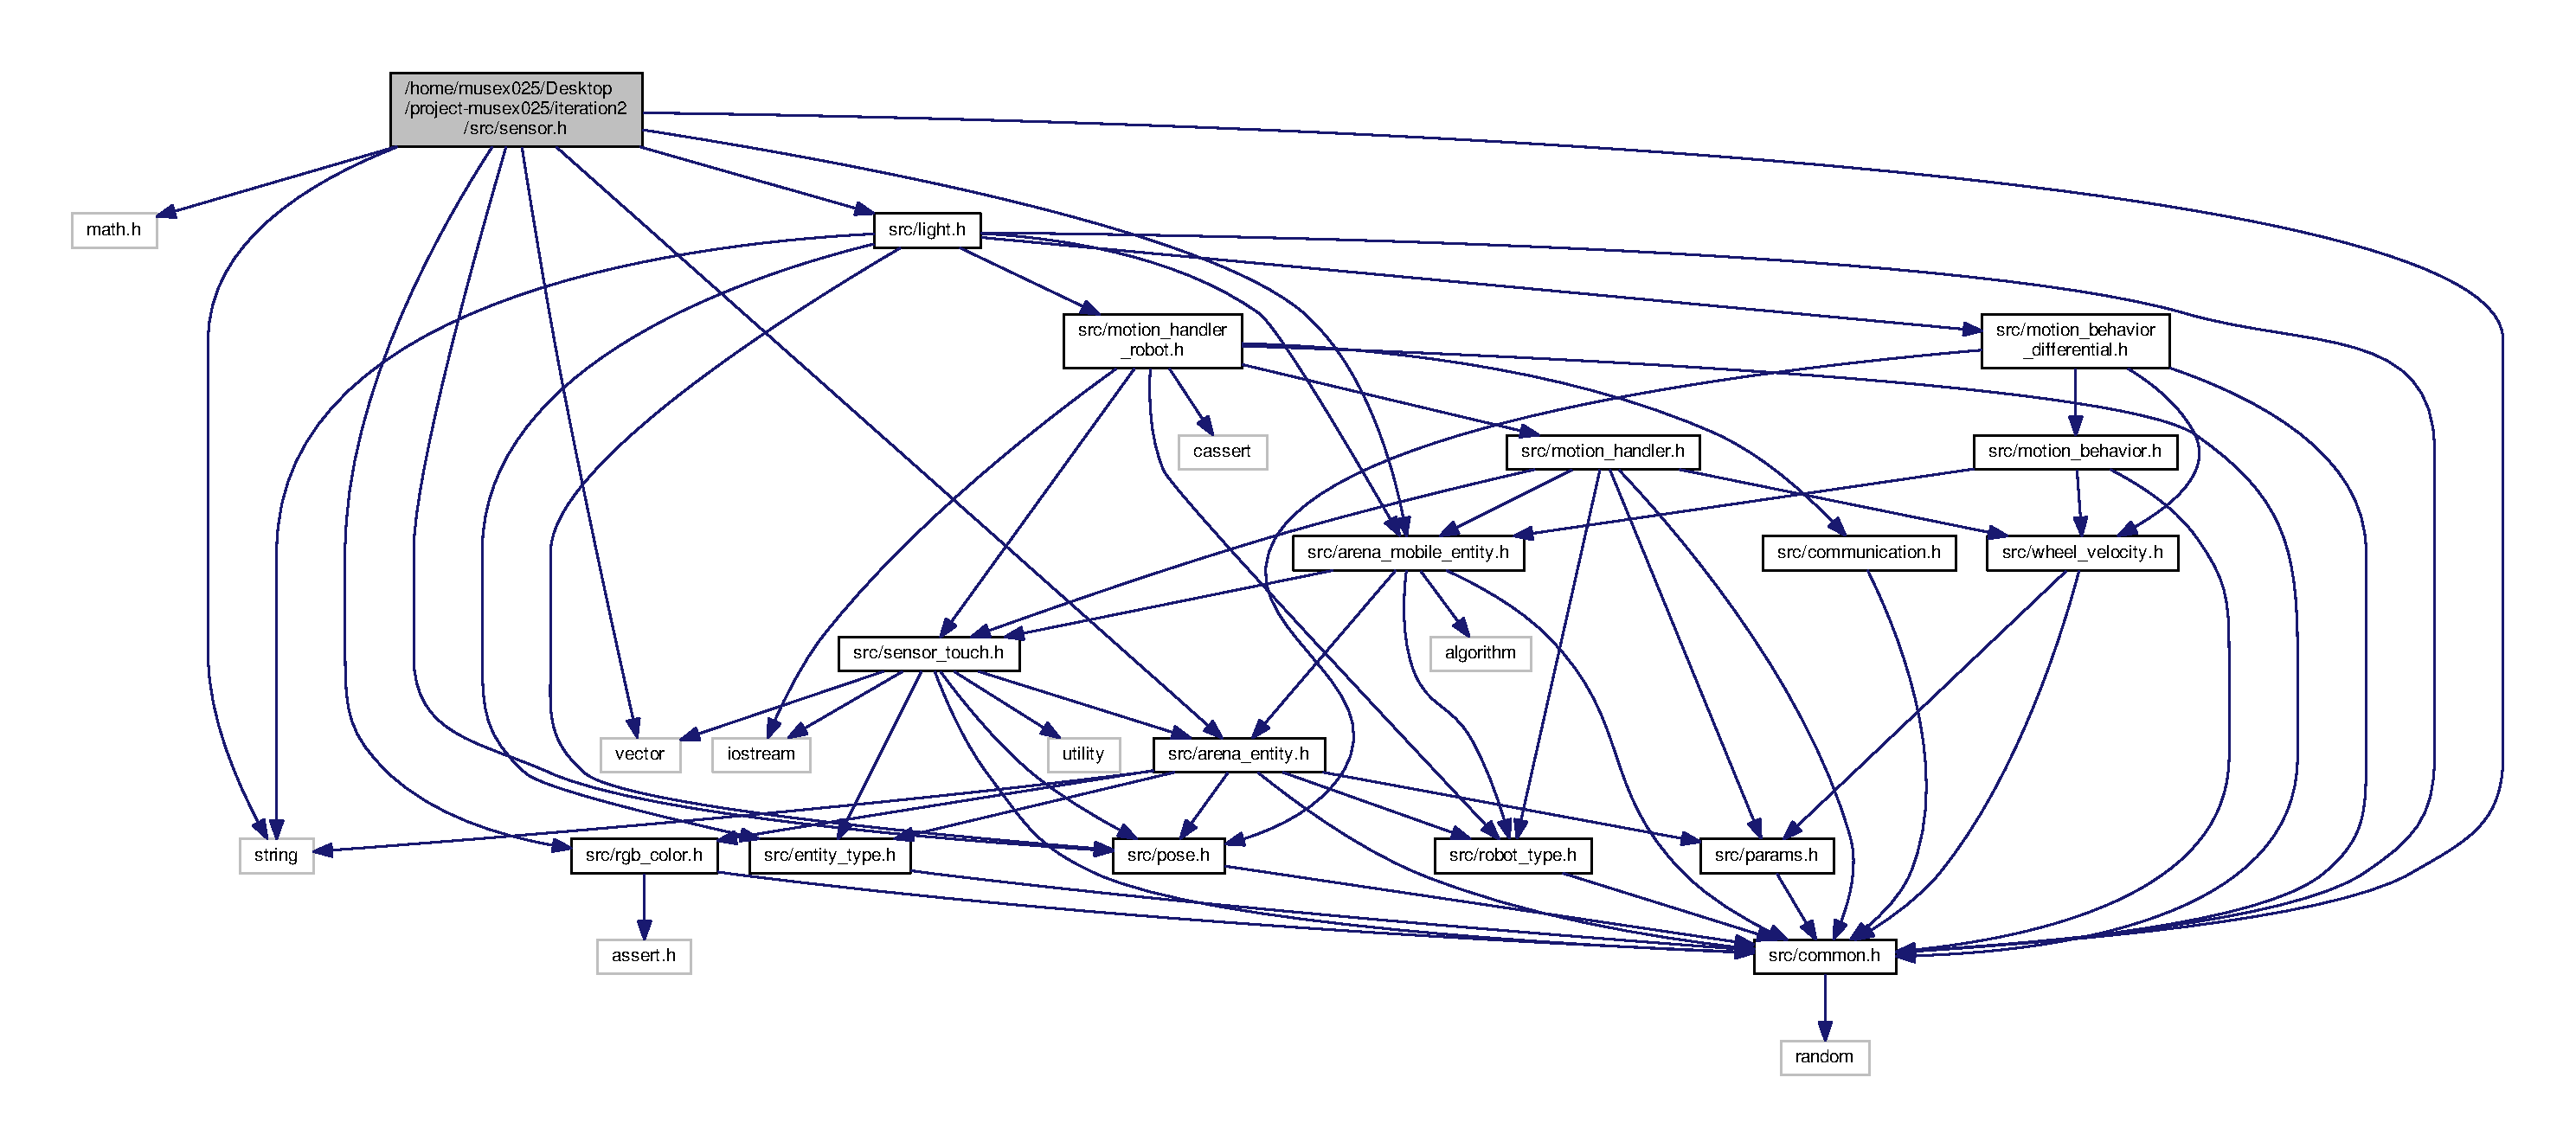
\includegraphics[width=350pt]{sensor_8h__incl}
\end{center}
\end{figure}
This graph shows which files directly or indirectly include this file\+:\nopagebreak
\begin{figure}[H]
\begin{center}
\leavevmode
\includegraphics[width=350pt]{sensor_8h__dep__incl}
\end{center}
\end{figure}
\subsection*{Classes}
\begin{DoxyCompactItemize}
\item 
class \hyperlink{classSensor}{Sensor}
\end{DoxyCompactItemize}
\subsection*{Functions}
\begin{DoxyCompactItemize}
\item 
{\bfseries N\+A\+M\+E\+S\+P\+A\+C\+E\+\_\+\+B\+E\+G\+IN} (csci3081)\hypertarget{sensor_8h_a5eaf22d0e7e2a0f12c6a660a6b011297}{}\label{sensor_8h_a5eaf22d0e7e2a0f12c6a660a6b011297}

\item 
{\bfseries N\+A\+M\+E\+S\+P\+A\+C\+E\+\_\+\+E\+ND} (csci3081)\hypertarget{sensor_8h_a0bc8eb973c3aef52acd7429898ace1cd}{}\label{sensor_8h_a0bc8eb973c3aef52acd7429898ace1cd}

\end{DoxyCompactItemize}


\subsection{Detailed Description}
\begin{DoxyCopyright}{Copyright}
2017 3081 Staff, All rights reserved. 
\end{DoxyCopyright}

\hypertarget{sensor__touch_8cc}{}\section{/home/musex025/\+Desktop/project-\/musex025/iteration2/src/sensor\+\_\+touch.cc File Reference}
\label{sensor__touch_8cc}\index{/home/musex025/\+Desktop/project-\/musex025/iteration2/src/sensor\+\_\+touch.\+cc@{/home/musex025/\+Desktop/project-\/musex025/iteration2/src/sensor\+\_\+touch.\+cc}}
{\ttfamily \#include $<$iostream$>$}\\*
{\ttfamily \#include \char`\"{}src/sensor\+\_\+touch.\+h\char`\"{}}\\*
Include dependency graph for sensor\+\_\+touch.\+cc\+:\nopagebreak
\begin{figure}[H]
\begin{center}
\leavevmode
\includegraphics[width=350pt]{sensor__touch_8cc__incl}
\end{center}
\end{figure}
\subsection*{Functions}
\begin{DoxyCompactItemize}
\item 
{\bfseries N\+A\+M\+E\+S\+P\+A\+C\+E\+\_\+\+B\+E\+G\+IN} (csci3081)\hypertarget{sensor__touch_8cc_a5eaf22d0e7e2a0f12c6a660a6b011297}{}\label{sensor__touch_8cc_a5eaf22d0e7e2a0f12c6a660a6b011297}

\item 
{\bfseries N\+A\+M\+E\+S\+P\+A\+C\+E\+\_\+\+E\+ND} (csci3081)\hypertarget{sensor__touch_8cc_a0bc8eb973c3aef52acd7429898ace1cd}{}\label{sensor__touch_8cc_a0bc8eb973c3aef52acd7429898ace1cd}

\end{DoxyCompactItemize}


\subsection{Detailed Description}
\begin{DoxyCopyright}{Copyright}
2017 3081 Staff, All rights reserved. 
\end{DoxyCopyright}

\hypertarget{sensor__touch_8h}{}\section{src/sensor\+\_\+touch.h File Reference}
\label{sensor__touch_8h}\index{src/sensor\+\_\+touch.\+h@{src/sensor\+\_\+touch.\+h}}
{\ttfamily \#include $<$utility$>$}\\*
{\ttfamily \#include $<$vector$>$}\\*
{\ttfamily \#include $<$iostream$>$}\\*
{\ttfamily \#include \char`\"{}src/common.\+h\char`\"{}}\\*
{\ttfamily \#include \char`\"{}src/pose.\+h\char`\"{}}\\*
{\ttfamily \#include \char`\"{}src/entity\+\_\+type.\+h\char`\"{}}\\*
{\ttfamily \#include \char`\"{}src/arena\+\_\+entity.\+h\char`\"{}}\\*
\subsection*{Classes}
\begin{DoxyCompactItemize}
\item 
class \hyperlink{class_sensor_touch}{Sensor\+Touch}
\begin{DoxyCompactList}\small\item\em Class representing a touch sensor. \end{DoxyCompactList}\end{DoxyCompactItemize}
\subsection*{Functions}
\begin{DoxyCompactItemize}
\item 
{\bfseries N\+A\+M\+E\+S\+P\+A\+C\+E\+\_\+\+B\+E\+G\+IN} (csci3081)\hypertarget{sensor__touch_8h_a5eaf22d0e7e2a0f12c6a660a6b011297}{}\label{sensor__touch_8h_a5eaf22d0e7e2a0f12c6a660a6b011297}

\item 
{\bfseries N\+A\+M\+E\+S\+P\+A\+C\+E\+\_\+\+E\+ND} (csci3081)\hypertarget{sensor__touch_8h_a0bc8eb973c3aef52acd7429898ace1cd}{}\label{sensor__touch_8h_a0bc8eb973c3aef52acd7429898ace1cd}

\end{DoxyCompactItemize}


\subsection{Detailed Description}
\begin{DoxyCopyright}{Copyright}
2017 3081 Staff, All rights reserved. 
\end{DoxyCopyright}

\hypertarget{sensor__type_8h}{}\section{src/sensor\+\_\+type.h File Reference}
\label{sensor__type_8h}\index{src/sensor\+\_\+type.\+h@{src/sensor\+\_\+type.\+h}}
{\ttfamily \#include \char`\"{}src/common.\+h\char`\"{}}\newline
\subsection*{Enumerations}
\begin{DoxyCompactItemize}
\item 
\mbox{\Hypertarget{sensor__type_8h_a213c434cb928c4ca22513e2302632435}\label{sensor__type_8h_a213c434cb928c4ca22513e2302632435}} 
enum {\bfseries Sensor\+Type} \{ \newline
{\bfseries k\+Love}, 
{\bfseries k\+Agressive}, 
{\bfseries k\+Coward}, 
{\bfseries k\+Sensor}, 
\newline
{\bfseries k\+Explore}
 \}
\end{DoxyCompactItemize}
\subsection*{Functions}
\begin{DoxyCompactItemize}
\item 
\mbox{\Hypertarget{sensor__type_8h_a5eaf22d0e7e2a0f12c6a660a6b011297}\label{sensor__type_8h_a5eaf22d0e7e2a0f12c6a660a6b011297}} 
{\bfseries N\+A\+M\+E\+S\+P\+A\+C\+E\+\_\+\+B\+E\+G\+IN} (csci3081)
\item 
\mbox{\Hypertarget{sensor__type_8h_a0bc8eb973c3aef52acd7429898ace1cd}\label{sensor__type_8h_a0bc8eb973c3aef52acd7429898ace1cd}} 
{\bfseries N\+A\+M\+E\+S\+P\+A\+C\+E\+\_\+\+E\+ND} (csci3081)
\end{DoxyCompactItemize}


\subsection{Detailed Description}
\begin{DoxyCopyright}{Copyright}
2017 3081 Staff, All rights reserved. 
\end{DoxyCopyright}

\hypertarget{wheel__velocity_8h}{}\section{src/wheel\+\_\+velocity.h File Reference}
\label{wheel__velocity_8h}\index{src/wheel\+\_\+velocity.\+h@{src/wheel\+\_\+velocity.\+h}}
{\ttfamily \#include \char`\"{}src/common.\+h\char`\"{}}\\*
{\ttfamily \#include \char`\"{}src/params.\+h\char`\"{}}\\*
Include dependency graph for wheel\+\_\+velocity.\+h\+:\nopagebreak
\begin{figure}[H]
\begin{center}
\leavevmode
\includegraphics[width=203pt]{wheel__velocity_8h__incl}
\end{center}
\end{figure}
This graph shows which files directly or indirectly include this file\+:\nopagebreak
\begin{figure}[H]
\begin{center}
\leavevmode
\includegraphics[width=350pt]{wheel__velocity_8h__dep__incl}
\end{center}
\end{figure}
\subsection*{Classes}
\begin{DoxyCompactItemize}
\item 
struct \hyperlink{structWheelVelocity}{Wheel\+Velocity}
\begin{DoxyCompactList}\small\item\em A simple representation of the position/orientation of an entity within the \hyperlink{classArena}{Arena}. \end{DoxyCompactList}\end{DoxyCompactItemize}
\subsection*{Functions}
\begin{DoxyCompactItemize}
\item 
{\bfseries N\+A\+M\+E\+S\+P\+A\+C\+E\+\_\+\+B\+E\+G\+IN} (csci3081)\hypertarget{wheel__velocity_8h_a5eaf22d0e7e2a0f12c6a660a6b011297}{}\label{wheel__velocity_8h_a5eaf22d0e7e2a0f12c6a660a6b011297}

\item 
{\bfseries N\+A\+M\+E\+S\+P\+A\+C\+E\+\_\+\+E\+ND} (csci3081)\hypertarget{wheel__velocity_8h_a0bc8eb973c3aef52acd7429898ace1cd}{}\label{wheel__velocity_8h_a0bc8eb973c3aef52acd7429898ace1cd}

\end{DoxyCompactItemize}


\subsection{Detailed Description}
\begin{DoxyCopyright}{Copyright}
2017 3081 Staff, All rights reserved. 
\end{DoxyCopyright}

%--- End generated contents ---

% Index
\backmatter
\newpage
\phantomsection
\clearemptydoublepage
\addcontentsline{toc}{chapter}{Index}
\printindex

\end{document}
